	%to make section start on odd page
	\newpage
	\thispagestyle{empty}
	\mbox{}
	\section{Numerical Methods/Analysis}
	
	\lettrine[lines=4]{\color{BrickRed}T}he numerical analysis is a mathematical discipline. It is interested in both theoretical foundations as the implementation methods to resolve by purely numerical calculations and empirical approach, mathematical analysis problems.\\
	
\textbf{Definition (\#\mydef):} "\NewTerm{Numerical Methods/Analysis}\index{Numerical Methods/Analysis}" is the study of algorithms or empirical scientific methods for solving or analysing mathematical continuous or discrete problems. This means that it mainly deals to respond numerically to real or complex variables questions like numerical linear algebra over the real or complex fields, looking for numerical solutions of differential equations and other problems occurring in the physical sciences or financial/statistical engineering.

Some continuous mathematical problems can be solved exactly by an algorithm. These algorithms are then named "\NewTerm{direct methods}\index{direct methods}". Examples are the elimination of Gauss-Jordan for solving a system of linear equations or the simplex algorithm of linear programming (see further below). However, for some problems no direct method are known (and is even proved that for a class of problems known as "NP complete" - see further below - there is no direct calculation with finished algorithm in a polynomial time). In such cases, it is sometimes possible to use an iterative method to attempt to determine an approximation of the solution. Such a method starts from a guessed value or roughly estimated one and finds successive approximations that should converge to the solution under certain conditions. Even when a direct method exists, however, an iterative method may be preferable because it is often more effective and often more stable (in particular it allows most often to correct minor errors in intermediate calculations).

	The use of numerical analysis has been greatly facilitated by modern computers. The Increasing availability and power of computers since the second half of the 20th century allowed the application of numerical methods in many scientific, technical and economic, often with revolutionary, accurate and significant effects.

	\begin{figure}[H]
		\centering
		\fbox{\includegraphics[scale=0.75]{img/computing/meaning_life.eps}}
	\end{figure}

In numerical simulations of physical systems (multi-physics), the initial conditions are very important in solving differential equations (see the various sections of this book where chaotic effects appears). The fact that we can not know them exactly implies that the results of calculations can never be perfectly accurate (we know this fact very well for the weather forecasting which is the most glaring example known). This effect is a consequence of the results of fundamental physics (based on pure mathematics) which demonstrates that we can not perfectly know a system by performing measurements since it directly disrupts it (Heisenberg uncertainty principle as see in the section of Quantum Wave Theory) and these disturbances are the subject of Chaos Theory (classical or quantum).

With new computer tools available in the early 21st century, it became practical and exciting to know the numerical methods to have fun with some softwares or programming languages (OpenGL, 3D Studio Max, Blender, Maple, MATLAB™, Mathematica, Comsol, R, C++, Python, etc.) to simulate 2D or 3D physical systems graphically.

	\begin{tcolorbox}[title=Remarks,colframe=black,arc=10pt]
	\textbf{R1.} Many numerical methods used in computer science are based on arguments which we have already been studied in other sections of this books. We won't come back on this methods.\\
	
	\textbf{R2.} This section being on the boundary between engineering and Applied Mathematics, we decided to give some application examples of developed tools with various programming languages or software.\\
	
	\textbf{R3.} Many of the techniques presented below are available as complete code in the C++ book \cite{oliveira2015practical} that we strongly recommend to the reader.
	\end{tcolorbox}	
	
	\textbf{Definitions (\#\mydef):}
	\begin{enumerate}
		\item[D1.]  An "\NewTerm{algorithm}\index{algorithm}" is a finite sequence of rules to be applied in a specific order in a finite number of data to arrive in a finite number of steps (including the amount, or conversely the execution time is defined by the term "\NewTerm{cost}\index{algorithm cost}") to a certain result, independently of the data type.
		
		\item[D2.] The algorithms are integrated into computers through "\NewTerm{programs}\index{programs}" (including stuff like "functions", "objects", "classes", "methods", "properties", "pointers", etc. but this is more related to a programming language course) that are the realization (implementation) of an algorithm using a given language (on a given architecture). This is the implementation of the principle.
	\end{enumerate}
	
	Axioms of programming (anecdotal):

	\begin{enumerate}
		\item[A1.] More we write code, more errors we will produce.
		
		\item[A2.] There are no programs without possible errors (due to the program itself, to the underlying electronics or most often to the user himself).
	\end{enumerate}
	
	\begin{tcolorbox}[title=Remarks,colframe=black,arc=10pt]
Basically there a minimum steps to follow when developing an algorithm and its corresponding code. A very good process to follow is the one proposed by the ISO/CEI 9126 norm.
	\end{tcolorbox}	

	When developing a scientific algorithm, it may be interesting, rigorous and even an obligation in very high level cases to analyze the "complexity" of the algorithm. Without going too far, let's see what it is exactly:
	
	\subsection{Computer Representation of Numbers}
	
	In a Computer numbers are represented by binary digits 0 and 1.
	Computers employ binary arithmetic for performing operations on
	numbers. Since it gets cumbersome to display large numbers in
	binary form computers usually display them in hexadecimal or octal
	or decimal system. All of these number systems are positional
	systems. In a positional system a number is represented by a set
	of symbols. Each of these symbols denote a particular value
	depending on its position. The number of symbols  used in a
	positional system depends on its 'base'. Let us now discuss about
	various positional number systems:
	
	\subsubsection{Decimal System}
	
	The decimal system uses 10 as its base value and employs ten
	symbols 0 to 9 in representing numbers. Let us consider a decimal
	number 7402 consisting of four symbols 7,4,0,2. In terms of base
	10 it can be expressed as follows.
	$$7402=7\times10^{3}+4\times10^{2}+0\times10^{1}+2\times10^{0}$$
	
	So each of the symbols from a set of symbols denoting a number is
	multiplied with power of the base (10) depending on its position
	counted from the right. The count always begins with 0.
	
	In general a decimal number $d_{m}d_{m-1}...d_{1}d_{0}$ consisting
	of $(m+1)$ symbols can be expressed as:
	$$
	d_{m}\times10^{m}+d_{m-1}\times10^{m-1}+....+d_{1}\times10^{1}+d_{0}\times10^{0}=\sum\limits_{i=0}^{m}
	d_{i}10^{i}
	$$
	where $0\leq d_{i}\leq 9$ with $i=0,1,\ldots, m$
	
	Similarly, a fractional part of a decimal number can be expressed
	as $\sum\limits_{i=1}^{m}d_{i}10^{-i}$
	
	\subsubsection{Binary system} 
	Binary system is the positional system 	consisting of two symbols i.e. 0,1 and '2' as its base. Any binary number $d_{m}d_{m-1}...d_{1}d_{0}$ actually represents a decimal value given by
	$$
	d_{m}2^{m}+d_{m-1}2^{m-1}+...+d_{0}2^{0}=\sum\limits_{i=0}^{m}
	d_{i}2^{i}
	$$
	where $d_{i}=0\quad or\quad 1, \quad i=0,1,..m. $
	
	Consider the binary number 10101. The decimal equivalent of 10101
	is given by
	\begin{eqnarray}
	(10101)_{2} & = & 1\times 2^{4}+0\times 2^{3}+1\times
	2^{2}+0\times 2^{1}+1\times 2^{0} \nonumber \\
	& = & 16+0+4+0+1=(21)_{10} \nonumber
	\end{eqnarray}
	
	Here are the representation of some integer positive values in binary notation:
	\begin{alignat*}{6}
	1&\qquad&1& \qquad\quad\qquad&  13&\qquad&1101&\qquad\quad\qquad &25&\quad&11001&\\
	2&&10&&  14&&1110&&   26&&11010&\\
	3&&11&&  15&&1111&&   27&&11011&\\
	4&&100&& 16&&10000&&   28&&11100&\\
	5&&101&& 17&&10001&&   29&&11101&\\
	6&&110&& 18&&10010&&   30&&11110&\\
	7&&111&& 19&&10011&&   31&&11111&\\
	8&&1000&&20&&10100&&  32&&100000&\\
	9&&1001&&21&&10101&&  33&&100001&\\
	10&&1010&&22&&10110&& 34&&100010&\\
	11&&1011&&23&&10111&& 35&&100011&\\
	12&&1100&&24&&11000&& 36&&100100&
	\end{alignat*}

	Notice that:
	\begin{itemize}
		\item The  number of different values representable in $n$ bits is  $2^n$,
		
		\item An $n$-bit binary number $X=x_{n-1}x_{n-2}\cdots x_1 x_0$ can represent  any integer value in the range $0 \le X \le 2^n-1$ (e.g., if $n=3$,  then $0 \le X \le 7$). Note that $n+1$ bits are needed to represent the value $X=2^n$.
		
		\item The highest (left-most) bit $x_{n-1}$ of an $n$-bit number is named the \NewTerm{most significant bit MSB}\index{most significant bit} and the lowest bit (right-most) $x_0$ the \NewTerm{least significant bit LSB}\index{least significant bit}".
	\end{itemize}
	\begin{figure}[H]
		\centering
		\includegraphics[scale=1]{img/arithmetics/binary_joke.jpg}
	\end{figure}
	
	\paragraph{Binary arithmetic}\mbox{}\\\\\
	Here are the addition facts that you need when additing numbers in binary notation:
	
	
	Doing binary addition is like doing decimal addition excepted that we work on a binary set. 
	\newcommand*{\carry}[1][1]{\overset{#1}}
	\newcolumntype{B}[1]{r*{#1}{@{\,}r}}
	\begin{equation*}
		\begin{array}{B3}
		    \carry 0 & \carry 1\carry 1\carry 0\carry 0 & \carry 1\carry 0\carry 01 \\
		      {} + 0 & 1111 & 1111 \\ \hline
		           1 & 1100 & 1000 \\
		\end{array}
	\end{equation*}
	Here are the subtractions facts that you need when subtracting numbers in binary notation:
	
	The fact that $10-1=1$ will lead to borrowing since you can not take $1$ from $0$ for a certain place value, and so you must borrow from the $1$ in the next place value, much like how you need to borrow in decimal notation:
	\begin{equation*}
		\begin{array}{B3}
		    		\carry 1 \carry 0\carry 01 \\
		      	{} - 0110 \\ \hline
		            0011 \\
		\end{array}
	\end{equation*}
	We will come back more in details on binary arithmetic during our study of Boolean algebra in the section of Logical Systems.
	
	\subsubsection{Hexadecimal System} 
	
	The Hexadecimal system is the 	positional system consisting of sixteen symbols, $0$,$1$,$2$...$9$,$A$,$B$,$C$,$D$,$E$,$F$, and '$16$' as its base. Here the symbols $A$ denotes $10$, $B$ denotes $11$ and so on. The decimal equivalent of the 	given hexadecimal number $d_{m} d_{m-1}...d_{0}$ is given by:
	
	 For example consider $(15ACB)_{16}$:
	
	We can convert a binary number directly to a hexadecimal number by grouping the binary digits, starting from the right, into sets of four and converting each group to its equivalent hexadecimal digit. If in such a grouping the last set falls short of four binary digits then do the obvious thing of prefixing it with adequate number of binary digit '$0$'. For example let us find the 	hexadecimal equivalent of $(111\;011\;0101\;0010\;1110)_{2}$:
	
	The vice versa is also true.
	
	\subsubsection{Octal System}  
	The octal system is the positional
	system that uses 8 as its base and $\{0,1,...7\}$ as its symbol set of size 8. The decimal equivalent of an octal number $(d_{m}d_{m-1}...d_{0})_{8}$ is given by:
	
	 For example consider $(6741)_{8}$:
	 
	
	We can get the octal equivalent of a binary number by grouping the binary digits, starting from the right, into sets of three binary digits and converting each of these sets to its octal equivalent.
	
	If such a grouping results in a last set having less number of digits it may be prefixed with adequate number of binary digit 0.
	
	As an example the octal equivalent of $(1010\;110\;111\;001)_{2}$.
	
	So we have:
	
	
	\pagebreak
	\subsubsection{Conversion of decimal system to non-decimal system:}
	To convert a decimal number to a number of any other system we should consider the integer and fractional parts separately and follow the following procedure:
	
	Conversion of integer part:
	\begin{enumerate}
		\item Consider the integer part of a given decimal number and divide it by the base $b$ of the new number system. The remainder will constitute the rightmost digit of the integer part of the new number.

		\item Next divide the quotient again by the base $b$. The remainder will constitute second digit from the right in the new system
	\end{enumerate}
	
	Continue this process until we end up with a zero-quotient. The last remainder is the leftmost digit of the new number.
	
	Conversion of fractional part:
	\begin{enumerate}
		\item Consider the fractional part of the given decimal number and multiply it with the base $b$ of the new system. The integral part of the product constitutes the leftmost digit of the fractional part in the new system.

		\item Now again multiply the fractional part resulting in step (a) by the base $b$ of the new system. The integral part of the resultant product is the second digit from the left in the new system.
	\end{enumerate} 
	
	Repeat the above step until we encounter a zero-fractional part or a duplicate fractional part. The integer part of this last product will be the rightmost digit of the fractional part of the new number.
	
	\begin{tcolorbox}[colframe=black,colback=white,sharp corners]
	\textbf{{\Large \ding{45}}Example:}\\\\
	We want to convert $54.45$ into its binary equivalent.\\
	
	\begin{enumerate}
		\item Consider the integer part i.e. $54$ and apply the steps listed under conversion of integer part i.e.

		\item conversion of fractional part:
		\vskip 10pt
	
		\begin{center}
			\begin{tabular}{ccccc}
			                  &   &  Product & integral part &
			Binary number \\ \hline $0.45$ $\times$ $2$   & = &  $0.90$    &   $0$ &
			$(.01\overline{1100})_2$ \\
			0.9 $\times$ 2   & = &  1.80    &    1 &  \\
			0.8 $\times$ 2   & = &  1.6     &    1 &  \\
			0.6 $\times$ 2   & = &  1.2     &    1 &  \\
			0.2 $\times$ 2   & = &  0.4     &    0 &  \\
			0.4 $\times$ 2   & = &  0.8     &    0 &  \\
			0.8 $\times$ 2   & = &  1.6     &    1 &  \\
			0.6 $\times$ 2   & = &  1.2     &    1 &  \\
			0.2 $\times$ 2   & = &  0.4     &    0 &  \\
			0.4 $\times$ 2   & = &  0.8     &    0 &  \\
			0.8 $\times$ 2   & = &  1.6     &    1 &  \\
			$\dots$          &   &  $\dots$ &    $\dots$ &  \\
			$\dots$          &   &  $\dots$ &    $\dots$ &  \\
			\hline
			\end{tabular}
		\end{center}
	\end{enumerate} 
	Therefore:
	
	and finally:
	
	\end{tcolorbox}
	
	Here the overbar denotes the repetition of the binary digits.
	
	Note: Using binary system as an intermediate stage we can easily convert octal numbers to hexadecimal numbers and vice-versa.
	\begin{tcolorbox}[colframe=black,colback=white,sharp corners]
	\textbf{{\Large \ding{45}}Example:}\\\\
	(a)$(423)_{8}=(100\quad 010\quad 011)_{2}$
	
	$\qquad\qquad\qquad=(0001\quad 0001\quad 0011)_{2}=(113)_{16}$
	
	(b) $(93.Af)_{16}$
	
	$\qquad\qquad\qquad=(1001\quad0011.\quad1010\quad1111)_{2}$
	
	$\qquad\qquad\qquad=(010\quad010\quad011.\quad101\quad011\quad110)_{2}$
	
	$\qquad\qquad\qquad=(223.536)_{8}$
	\end{tcolorbox}
	
	In the above two examples we have grouped the binary digits suitably either to quadruplets or triplets to convert octal to hexadecimal and hexadecimal to octal numbers respectively.



	\pagebreak	
	\subsection{Algorithm Complexity }

\textbf{Definition (\#\mydef):} The "\NewTerm{complexity}\index{complexity}" of an algorithm is the measure of the number of fundamental operations it performs in the worst case on a dataset.

Measure the exact complexity is most of time irrelevant because often too complex given the size of the programs (too big algorithms). To avoid calculating in detail the complexity of an algorithm, we identify the fundamental operations. These basic operations can be: an assignment, a comparison between two variables, an arithmetic operation between two variables, etc.

Thus, the classical used hypothesis for the calculation of the complexity are:

	\begin{enumerate}
		\item[H1.] The four fundamental operations have the same time cost: $+ \equiv - \equiv \times \equiv \div$
		\item[H2.] A memory access has a cheaper time cost than an arithmetic operation.
		\item[H3.] A comparison check has a cheaper time cost than an arithmetic operation.
		\item[H4.] We work with only one single processor.
	\end{enumerate}
	
\textbf{Definitions (\#\mydef):}
	\begin{enumerate}
		\item[D1.] We note $D_n$ the sets of data of size $n$ and $T(n)$ the cost (in time) of the algorithm on the data or the data set of size $n$.
		\item[D2.] The "\NewTerm{complexity at the best}\index{complexity at the best}" is given by the function:
			
		This is the smallest time that will need an algorithm to run on a data set (lines of code) of fixed size, here equal to $n$, that the cost (duration) execution is $C(d)$. This is a lower bound on the complexity of the algorithm on a data set of size $n$.
		\item[D3.] The "\NewTerm{complexity at worst}\index{complexity at worst}" (the most interesting for the practitioner because it is the one to minimize!):
			
		This is the biggest time that will need an algorithm to run on a data set (lines of code) of fixed size, here equal to $n$, that the cost (duration) execution is $C(d)$. This is a upper bound on the complexity of the algorithm on a data set of size $n$. The algorithm will always finish at this time or before but never after.
		\item[D4.] The "\NewTerm{average complexity}\index{average complexity}":
			
This is the average of the complexities of the algorithm on the data sets of size n (strictly speaking, we must obviously take into account the probability of occurrence of each of the data sets). This average reflects the general behavior of the algorithm if extreme cases are rare or complexity varies slightly depending on the data. However, the complexity in practice on a particular data set may be significantly greater than the average complexity; in this case the average complexity does not give a good indication of the behavior of the algorithm.		
		\item[D5.] The "\NewTerm{order of complexity}\index{order of complexity}" is defined as the number worst complexity at worst of an algorithms that contains several terms (additions or subtractions) so that we only keep the term that is growing the fastest. Thus, an algorithm having a complexity of type:
			
will be said to have a complexity of order $\mathcal{O}(n!)$
	\end{enumerate}

	\begin{tcolorbox}[colframe=black,colback=white,sharp corners]
\textbf{{\Large \ding{45}}Examples:}\\\\
Consider $N$ as the size of the data. For a decimal number this is the numbers $N$ of digits. Consider two decimal numbers like $0.a_1a_2a_3...$ and $0.b_1b_2b_3...$\\

E1. Addition has linear complexity because in developed way addition is expressed as (\SeeChapter{see section Numbers}):\\
	

E2. Multiplication has quadratic complexity because in developed way multiplication is expressed as:\\
	
	\end{tcolorbox}

\textbf{Definition (\#\mydef):} An algorithm is said to be "\NewTerm{optimal algorithm}\index{optimal algorithm}" if its complexity has the minimal complexity among all other algorithms in its class.

As we made it understand implicitly earlier, we focus almost exclusively on the time complexity of the algorithms. Sometimes it is interesting to focus on other of their characteristics, such as space complexity (size of the memory used), the bandwidth required, etc.

For the result of the analysis of an algorithm to be relevant, we must have a model of a machine on which the algorithm will be implemented (as a program). We usually take as a reference, the "random access machine (RAM)" with a single processor where instructions are executed one after the other, without concurrent operations and without stochastic processes (in contrast to possible future quantum computers).

Most common algorithms can be classified into a number of broad classes of complexity whose order $\mathcal{O}$ varies somehow:
	\begin{enumerate}
		\item The algorithms with "\NewTerm{constant complexity $\mathcal{O}(1)$}\index{complexity!constant complexity}" that just do a boolean control (comparison).
		
		\item The algorithms with "\NewTerm{linear complexity $\mathcal{O}(n)$}\index{complexity!linear complexity}" and those in complexity in $\mathcal{O} (n log (n))$ that are considered as fast.
		
		\item The algorithms with "\NewTerm{"polynomial complexity in $\mathcal{O}(n^k)$}\index{complexity!polynomial complexity}" (for $k>3$ are considered as slow).
		
		\item The algorithms with "\NewTerm{sub-linear complexity}\index{complexity!sub-linear complexity}" whose complexity is usually of the order $\mathcal{O}(\log (n))$
		
		\item The algorithms with "\NewTerm{factorial complexity}\index{complexity!factorial complexity}" whose complexity is usually of the order $\mathcal{O}(n!)$
	\end{enumerate}
and so on... (we give here definition only for complexity for which we already have given a detailed example or will give examples further below).

It is important to see that (focusing only on complexities we have seen with examples or will see later below):
	

	\begin{tcolorbox}[title=Remark,colframe=black,arc=10pt]
In practice a good complexity is considered as being of order $\mathcal{O}(n^k)$ for $k>3$. Poor complexity is considered as being of type $\mathcal{O}(e^n),\mathcal{O}(n!)$ or equation.
	\end{tcolorbox}

We already saw above an example with linear complexity (addition of scalars) and of polynomial (quadratic) complexity (with multiplication of scalars).


Let us see some other very common examples. The first example use the results of the previous examples:

	\begin{tcolorbox}[colframe=black,colback=white,sharp corners]
\textbf{{\Large \ding{45}}Example:}\\\\
	E1. Evaluation of a polynomial:
	
	The direct estimate of the value of $P(x)$ leads to a complexity:
	
	E2. Another important example is the inversion matrix problem that is used a lot in supercomputer megaflops benchmark (sometimes named "\NewTerm{LINPACK test}\index{LINPACK test}". As you can see in the MATLAB companions book there is a division by $n^3$ as the matrix inversion of of complexity order of $n^3$. Indeed:\\
	
	At the beginning, when the first row has length $n$, it takes $n$ 
   operations to zero out any entry in the first column (one division, 
   and $n-1$ multiply-subtracts to find the new entries along the row 
   containing that entry. To get the first column of zeroes therefore 
   takes $n(n-1)$ operations.\\
   
    In the next column, we need $(n-1)(n-2)$ operations to get the second 
   column zeroed out.\\

   In the third column, we need $(n-2)(n-3)$ operations.\\
   
   The sum of all of these operations is:
   
	which goes as $\mathcal{O}(n^3)$. 
	
	\end{tcolorbox}
	Thanks to William George Horner we have a more efficient algorithm that uses a factorization of the polynomial in the form:
	
We can see almost easily that this factorization holds the same number of additions to $(n)$ but reduces the number of multiplications to $(n)$.

The resulting complexity is $\mathcal{O} (n)$. The gain is unquestionably important. In addition, this  factorization avoids computing power.

Let us see now another well know example that almost all students that have learn scripting a little bit have experiences:

	\begin{tcolorbox}[colframe=black,colback=white,sharp corners]
\textbf{{\Large \ding{45}}Examples:}\\\\
The famous example of algorithmic complexity is the search for an  information in a sorted column (list). A simple algorithm named "dichotomous search" is to take the cell to mid-column and see if we find the desired value. Otherwise, research must continue on the same method in the top or bottom of the column (depending on the lexicographical order).\\\\
The algorithm is recursive and allows at each step, to divide by two the size of the search space.\\\\
If this size is initially of $n$ cells in the column, it is of size $\dfrac{n}{2}$ in step 1, of size $\dfrac{n}{2^2}$ in step 2, and more generally of size $\dfrac{n}{2^k}$ in step $k$.\\\\
At worst, the search ends when there is only one cell in the column to explore, i.e. when $k$ is such that $n<2^k$.\\\\
We deduce the maximum number of steps: it is the smallest $k$ such that $n<2^k$, written in another way $\log_2(n)<k$, i.e. the sub-linear complexity:
	
	\end{tcolorbox}
The result of this last example is to compared with a sequential search (useful when sorting is too costly in resources). For example, in a column of 25,000 data the complexity is $\mathcal{O}(n)$ thus 25,000 while with the dichotomous method, the sub-linear complexity gives $\log_2(25,000)=15$. The gain is considerable (at the condition that data is sorted)!

Other complexity that the reader must absolutely know are some elementary Linear Algebra calculations (see the section of the same name)! So without proof (because normally trivial given the previous examples) if we consider two square matrices $A$ and $B$ of dimensions $n$ the main operations have the following complexities:
	\begin{itemize}
		\item Read the components (nested loops): $\mathcal{O}(n^2)$
		\item Calculation of the trace: $\text{tr}(A)=\displaystyle\sum_{i=1}^{n}a_{ii}\rightarrow \mathcal{O}(n)$ 
		\item Addition $A+B=C$ so that $c_{ij}=a_{ij}+b_{ij}\rightarrow \mathcal{O}(n^2)$
		\item Product $A\cdot B=c$ so that $c_{ij}=\displaystyle\sum_{k=1}^na_{ik}b_{kj}\rightarrow \mathcal{O}(n^3)$
		\item Determinant (by the direct method of Cramer as detailed in the section of Linear Algebra). We can thus show that the complexity order of the determinant of a square matrix of dimensions $n$ is $n$ products, $n-1$ additions plus $n$ times the complexity of the determinant of a matrix of dimensions $n-1$ so that finally we have: $\text{det(A)}=\mathcal{O}(n\cdot n!)$
	\end{itemize}
Assuming that the computer performs an elementary operation in equation seconds (which is already a good computer), we obtain the following calculations time for several values of $n$ for the determinant:

		
hence the need to make sometimes a time complexity calculation before starting an algorithm (unless you are working exclusively for future generations, provided that there will still be future generations...).

\subsubsection{NP-Completude}

We will introduce now for the general culture the concept of "\NewTerm{NP-completeness}\index{NP-completeness}", that is to say that we will try to define without too much formalism (as usual in this book).

First let us introduce two non-formal definitions of a Turing machine.

\textbf{Definitions (\#\mydef):}

\begin{enumerate}
	\item[D1.] An algorithm is said to be a "\NewTerm{deterministic Turing machine}\index{deterministic Turing machine}" when the set of its rules prescribes at most one action to be performed for any given situation.
	
	\item[D2.] A "\NewTerm{non-deterministic Turing machine}\index{non-deterministic Turing machine}" may have a set of rules that prescribes more than one action for a given situation. For example, a non-deterministic Turing machine may have both "If you are in state 2 and you see an 'A', change it to a 'B' and move left" and "If you are in state 2 and you see an 'A', change it to a 'C' and move right" in its rule set.
\end{enumerate}

Now let us define what type of problems are frequently considered:

\textbf{Definitions (\#\mydef):}

\begin{enumerate}
	\item[D1.] "\NewTerm{Logarithmic problems L}\index{problem!Logarithmic problems L}" contains all algorithms (problems) that can be solved by a deterministic Turing machine using a logarithmic amount of computation time.
	
	\item[D2.] "\NewTerm{Polynomial problems P}\index{problem!Polynomial problems P}" contains all algorithms (problems) that can be \underline{solved} by a deterministic Turing machine using a polynomial amount of computation time.
	
	\item[D3.] "\NewTerm{Non-deterministic polynomial time problems NP}\index{problem!Non-deterministic polynomial time problems NP}" are the set algorithms (problems) where the result instances can be \underline{controlled} in a polynomial time complexity by a non-deterministic Turing machine. 
\end{enumerate}

It should be noted at this stage of the discussion that the class P is included in the NP class so that $\text{P} \subset \text{NP} $. Indeed if we know a polynomial algorithm to solve a problem then we can at worst check the solution with a polynomial complexity algorithm also.

	But a difficult question is the following reciprocal: if a problem is NP (known solution can be controlled in polynomial time) but it seems we can not found yet an algorithm in a polynomial time (or less) to find the solution, does it always exist a polynomial algorithm to find the solution so that $P=NP$ that thus bring us to write  $\text{P} \subseteq \text{NP}$?
	
	In other words: If the solution of a problem can be quickly verified as being the correct one, can the solution also be found quickly?
	\begin{tcolorbox}[colframe=black,colback=white,sharp corners]
	\textbf{{\Large \ding{45}}Examples:}\\\\
	E1. The problem of finding a Hamiltonian cycle (cycle that passes once and only once by all the vertices of the graph - see section Graphs Theory) in a graph belongs to NP since, given a known cycle it is trivial to check in linear time $\mathcal{O}(n)$ it contains a well and once each vertex but found the cycle is at worst a factorial complexity $\mathcal{O}(n!)$.\\
	
	E2. Factoring an integer $n$ in product of prime factors (important in cryptography) is an NP problem. Indeed, given the prime factors $p_1,p_2,...,p_n$ it is trivial to control the solution $n=p_1,p_2,...,p_n$ as it is of order $\mathcal{O}(n^2)$. But we do not know if it exist a polynomial algorithm to find the prime numbers (to found the solution). So we do not know if the problem of finding prime numbers of an integer is a P-problem.
	\end{tcolorbox}
	
	\begin{tcolorbox}[title=Remark,colframe=black,arc=10pt]
Apparently (we were not able to find the proof of this result and neither had opportunity to do so) the complexity of the best factorization algorithm for prime numbers is in the year 2007 of the type:
	
therefore there is still work to do (if a reader could provide us with the details that led to this result, we are interested).
	\end{tcolorbox}

A problem $x$ that is in NP is also in NP-Complete if and only if every other problem in NP can be quickly (i.e.. in polynomial time) transformed into $x$.

In other words a problem $x$ is "\NewTerm{NP-Complete NPC}\index{NP-Complete NPC}" if:
	\begin{enumerate}
		\item $x$ is in NP
		\item Every problem in NP is reducible to $x$
	\end{enumerate}
So, what makes NP-Complete so interesting is that if any one of the NP-Complete problems was to be solved quickly, then all NP problems can be solved quickly.

A NPC problem is complete in that it contains most of the complexity of problems belonging to NP, and a polynomial solution to this problem involves a polynomial solution to all NP type problems.

In other words: NPC problems have an exponential complexity and they all have the same complexity class (modulo polynomials).

Finally, what is important to understand and retain about this idea is that if we find one day a polynomial algorithm for one of these really difficult problems that are the NPC problems, then in one stroke NP becomes equal to P and all difficults problems become easy such that 
	
In other words: can we find in a polynomial time what can be proved (controlled) in polynomial time?

	\begin{tcolorbox}[title=Remark,colframe=black,arc=10pt]
This issue is so important in computing science to reduce energy consumptions and time computations that it belongs (arbitrarily) to the 7 millennium problems, whose resolution is prized \$1 million  by the Clay Mathematic Institute. 
	\end{tcolorbox}
	
Ok this definitions given let us now study of some typical applications of numerical methods which are very often used in the industry. We will go from simple to more complicated and not forgetting that many methods that are not in this section can sometimes be found in other sections of the book!

\subsection{Integer Part}

The biggest integer less than or equal to a real number x is expressed in this book by $[x]$, which will be read "\NewTerm{integer part of $x$}\index{integer part}" and according to the norm ISO 80000-2:2009 \textit{Mathematical signs and symbols to be used in the natural sciences and technology} it should denoted as: $\text{int} \; x$.

The number $M$ is an integer if and only if $[M] = M$. Similarly, the natural number $A \in \mathbb{N}$ is divisible in the natural set by the natural number $B \in \mathbb{N}$ if and only if:
	
We also denote by $\left\lbrace x\right\rbrace $ the fractional part of $x$ such that:
	
That is to say:
	
with $\mid \left\lbrace x\right\rbrace \mid < 1$
Consider $x,y \in \mathbb{R}$. Then we have the following properties (normally most of them don't need any proof):
	\begin{enumerate}
		\item[P1.] $[x]\leq x <[x]+1\Leftrightarrow 0\leq x-[x] <1$
		\item[P2.] $[x]=\displaystyle\sum_{n\leq x} 1$ for $x \geq 0$
		\item[P3.] $[x+m]=[x]+m$ if $m \in \mathbb{Z}$
		\item[P4.] $[x]+[y] \leq [x+y] \leq [x]+[y]+1$
		\begin{dem}
			A reader asked for the proof of this property. So let us see how to proceed. First we write:
			
		where $n,m \in \mathbb{Z}$ and where $0 \leq \theta < 1$ and $0 \leq \phi <1$. Thus:
			
			By writing $x=n+\theta$, where $0\leq 0 <1$, we have:
			
			where $0 < 1 -\theta \leq 1$.
			It follows that:
			
			if $\theta = 0$ and:
			
			if $0<\theta<1$.
			\begin{flushright}
				$\square$  Q.E.D.
			\end{flushright}
		\end{dem}
		\item[P5.] $[-x]=-[x]$ if $x \in \mathbb{Z}$ otherwise $[-x]=-[x]-1$ if $x \not\in \mathbb{Z}$
			\begin{dem}
			 The proof is already given at the end of the proof of property P4.
			\begin{flushright}
				$\square$  Q.E.D.
			\end{flushright}		
			\end{dem}
		\item[P6.] $\left[\dfrac{[x]}{m}\right]=\left[\dfrac{x}{m}\right]$ if $m \in \mathbb{N}$ 
			\begin{dem}
				For this proof we will write:
				
				where $0 < \theta <1$
				and:
				
			where $0 \leq r < m-1$ (\SeeChapter{see section Number Theory}). So we get:
				
				because $0 \leq r + \theta \leq m$. Besides :
				
				and thus we have the expected result.
				\begin{flushright}
					$\square$  Q.E.D.
				\end{flushright}
			\end{dem}

		\item[P7.] If $a \in \mathbb{N}$ then $\left[\dfrac{x}{a} \right]$ represents the number of integers less than or equal $x$ that are divisible by $a$.
			\begin{dem}
				For the last part, we observe that if $a, 2a,...,ma$ are all positive integers $\leq x$ that are divisible by $a$, it suffices to prove that $\left[\dfrac{x}{a}\right]=m$. 
				
				Since $(m+1)a>x$, then:
					
				That is to say:
					
				and thus we have the expected result.					
				\begin{flushright}
					$\square$  Q.E.D.
				\end{flushright}			
			\end{dem}
	\end{enumerate}
		\begin{tcolorbox}[title=Remark,colframe=black,arc=10pt]
The rounding method of real values will be given in the section on Economy.
	\end{tcolorbox}
	
	\subsection{Heron's Square Root Algorithm}
	
	One of the first things that many people learn in an introduction to Computer Sciences course is the algorithm for calculating the square root of a number. 
	
	There is such a simple algorithm for this purpose named "\NewTerm{Heron's algorithm}\index{Heron's algorithm}" or "\NewTerm{algorithm of Heron of Alexandria}\index{algorithm of Heron of Alexandria}" which converge to the value of this square root.
	
	Thus want to calculate the square root:
		
	\begin{dem}
		Here is a pseudo-proof because historically the algorithm was built on purely intuitive considerations (since 100 BC algebra did not exist...). In high-school classes the result is given as a definition and just convergence is observed.
		
		So for the demonstration, we will proceed as follows:
			
			And the trick is to write:
				
				\begin{flushright}
					$\square$  Q.E.D.
				\end{flushright}
	\end{dem}
	
		\begin{tcolorbox}[colframe=black,colback=white,sharp corners]
\textbf{{\Large \ding{45}}Example:}\\\\
We want to calculate:
	
	We take $A=10$ and this gives us the following table of iterations:
	
			
	\end{tcolorbox}

	In the case of the cubic root, the proof is similar and we obtain:
	
	
	and so on...
	
	To conclude it is perhaps interesting to know that the reader can find in the section of Number Theory the method used in the antiquity (at least an analogy) using continued fractions.
	
		\pagebreak
		\subsection{Archimedes Algorithm}
	
	The calculation of the universal constant "pi" denoted by $\pi$ is certainly the algorithm with the greatest interest since we found this constant almost everywhere in physics and mathematics (there are numerous books on the subject available on the market).
	
	We recall that we did not give the value of $\pi$ in the section on Geometry or in other sections of this book until now. So we will now tackle this task.
	
	We define in geometry the number named "pi", independently of the metric used, as the ratio of half the circumference of a circle with its radius such that:
	
	It seems that we own the first algorithm of the calculation of this constant by Archimedes (287-212 BC.) and whose proof is given below:
	\begin{dem}
		Consider an $n$-polygon inscribed in a circle:
		\begin{figure}[H]
			\begin{center}
			\includegraphics[scale=0.75]{img/computing/archimedes_algorithm.eps}
			\end{center}	
			\caption{The illustrated principle of Archimedes algorithm}
		\end{figure}
	The principle of Archimedes algorithm is as follows:
	
	Given the perimeter of a regular polygon of $n$ sides inscribed in a circle of radius $1/2$ we can see in the figure above that by induction (\SeeChapter{see section Trigonometry}):
	
	With have for the perimeter of an $n$-polygon:
	
	and:
	
	With:
	
	Therefore:
	
	Therefore:
	
	We then just need a computer and several iterations to evaluate with a good accuracy the value of $\pi$. Obviously, we use the Heron algorithm to calculate the square root...
	\begin{flushright}
		$\square$  Q.E.D.
	\end{flushright}
	\end{dem}
	
	\begin{tcolorbox}[title=Remark,colframe=black,arc=10pt]
	There are a large number of algorithms to compute $\pi$. The one shown above, without being the most aesthetic, seems historically to be the first and most simple one.
	\end{tcolorbox}
	
	\pagebreak
	\subsection{Euler's Number $e$}
	
	Including the constant $\pi$, there are many other important mathematical constant that we need to generate with a computer (nowadays most constant values are stored as is and are not recalculated automatically). Among them, is the "\NewTerm{Euler number}\index{Euler number}" denoted by $e$ (\SeeChapter{see section Functional Analysis}). Let's see how to calculate this number.
	
	Consider the Taylor series (\SeeChapter{see section on Sequences and Series}) for an infinitely differentiable function $f$ given by:
	
	As (\SeeChapter{see section Differential and Integral Calculus}):
	
	Therefore we have:
	
	So finally:
	
	This relation provides an easy algorithm to calculate the Euler number to a given order $n$ of precision.

	\subsection{Stirling's factorial approximation}
	Obviously, the factorial may be calculated with a simple iteration. However, this kind of method generates an exponential complexity algorithm which is not the best. Then there exists another method:

	In mathematics, Stirling's approximation (or Stirling's formula) is an approximation for factorials. It is a very powerful approximation, leading to a very useful in Statistical Mechanics (see section of the same name). 

	There are various approach that lead to different results. We will focus here on the only one that we will use later in theoretical physics and that is the worst easiest approximation.
	
	Either the definition of the factorial:
	
	
	And according to the properties of logarithms:
	
	
	If $n$ is very large (but very large) then the previous sum can be approximately written as an integral:
	
	
	Solving this integral we get (\SeeChapter{see section Differential and Integral Calculus})
	
	
	When $n \gg 1$, the lower limit is negligible and then (approximation that will be very useful in the section of Statistical Mechanics):
	
	\begin{figure}[H]
		\centering
		\includegraphics[scale=0.7]{img/computing/stirling_factorial_approximation.jpg}
		\caption{Comparison of logarithmic formulations using Stirling formula}
	\end{figure}
	
	After a small elementary simplification, we obtain:
	
	
	The latter relation is useful of course only if we assumes that Euler's constant is a value stored in the machine...
	
	Let Consider the Gamma function (\SeeChapter{see section Differential and Integral Calculus}):
	
	and recall that for integers $\lambda$ we have:
	
	We get:
	
	Substituting $y=t/\lambda$ and letting $g(x)=y-\log (y)$ We get: 
	
	Now we will use Laplace's method of integration (\SeeChapter{see section Differential and Integral Calculus}) and for this we we differentiate twice and get:
	
	so that $y^*=1,g(y^*)=1$ and $g''(y^*)=1$. Laplace's method now
	yields to:
	
	The relation:
	
	which is known as "\NewTerm{Stirling's improved formula}\index{Stirling's improved formula}".
	
	\pagebreak
	\subsection{Linear System of Equations}
	
	There are many methods for solving systems of linear equations. Most of them have been developed to address particular systems. We will here study for the moment only one named the "\NewTerm{Gauss reduction method}\index{Gauss reduction method}" or "\NewTerm{Gauss pivot}\index{Gauss pivot}" or "\NewTerm{Gauss reduction algorithm}\index{Gauss reduction algorithm}" which is well suited for solving small systems of linear equations (up to 50 unknown).
	
	\begin{tcolorbox}[title=Remarks,colframe=black,arc=10pt]
	\textbf{R1.} The validity of some of the operations that we will perform here to solve linear systems is proved in the section on Linear Algebra. In fact, to be brief, the whole method use vector spaces whose columns are linearly independent vectors.\\

	\textbf{R2}. Recall that linear systems admit a solution if and only if the rank of the augmented matrix is less than or equal to the number of equations (\SeeChapter{see section Linear Algebra}).
	\end{tcolorbox}
	
	\subsubsection{One equation with on unknown}
	
	We begin for sure with the easiest and smallest possible example... of one equation with one unknown:
	
	Where $a$ and $b$ are the coefficients of the equation and $x$ is unknown. Solving this equation consists to determine $x$ is according to $a$ and $b$. If $a$ is not equal to $0$ then:
		
	is the solution of the equation. If $a$ is equal to zer0 and if $b$ is different from $0$ then the equation above admits no solution. If $a$ and $b$ are equal to zero, then the equation has infinitely many solutions.
	
	\subsubsection{Two equations with two unknowns}
	
	A linear system of two equations with two unknowns can be written as we know:
		
		Where $a_{11},a_{12},a_{21},a_{22}$ are the coefficients of the equations, $x_1$ and $x_2$ are the unknowns.
		
		\begin{tcolorbox}[title=Remark,colframe=black,arc=10pt]
The above-used notations have nothing to do with the tensor calculus!
		\end{tcolorbox}	
		
		To solve the system following the algorithm that interest us we proceed as follows:
		
		Using elementary algebraic manipulations (addition or subtraction of the various equalities between themselves - operations authorized by the linear independence of vectors-lines) we transform the system into another with one unknown less for one of the both equations given by (for example):
		
		The transformation between the two systems:
		
		is simply done by multiplying each coefficient of the first equality by $\dfrac{a_{21}}{a_{11}}$ and subtracting the second line with the resulting equation. This procedure is named "\NewTerm{row reduction}\index{row reduction}" or "\NewTerm{Gaussian elimination}\index{Gaussian elimination}". 
		
		In our case, the element $a_{11}$ is named the "\NewTerm{pivot}\index{pivot}" or "\NewTerm{leading coefficient}\index{leading coefficient}". In others words, if the $L_i$ is the notation for the each line number of the system, what we made is:
		
		Then, we solve the equation with only one unknown:
		
		We can therefore conclude with:
		
		But this is not the real algorithm. The real one use the augmented form:
		
		 Now we apply $L_2-\dfrac{a_{21}}{a_{11}}L_1\rightarrow L_2$ and $L_1-\dfrac{a_{12}}{a_{22}}L_2 \rightarrow L_1$ such that:
		
		As you can see the matrix has been put in diagonal form!
		Now to continue, we write:
		
		
		Now we just apply $\dfrac{1}{a_{11}^{'}}L_1 \rightarrow L_1$ and  $\dfrac{1}{a_{12}^{'}}L_2 \rightarrow L_2$ such that:
		
		Finally:
		
		
		\subsubsection{Three equations with three unknowns}
	Now consider the case of the linear systems of three equations with three unknowns:
		
	We can subsequently by elementary operations (see section Linear Algebra and the previous case) reduce this linear system in the following echelon form system:
		
		And therefore we can trivially solve the last line:
		
		And afterwards the second line:
		
		And finally:
		
		Let us return to the systems transformations. It is carried out in two stages:
		\begin{enumerate}
			\item In the first line, we choose $a_{11}$ as the pivot and we eliminate the coefficients $a_{21}$ and $a_{31}$ as follows:
			
			We have to multiply each coefficient of the first line by $\dfrac{a_{21}}{a_{11}}$ and subtract this result of the second line and therefore $a_{21}$ disappears.
			
			Similarly, by multiplying the coefficients of the first line by $\dfrac{a_{31}}{a_{11}}$, and subtracting the result obtained from the third line, $a_{31}$ disappears.
			
			The linear system of equations can therefore be written as:
			
			\item The second step is to treat the linear system of two equations with two unknowns formed by the second and third lines of the previous system and that, in choosing $a_{22}^{'}$ as pivot. This method of resolution can seem complicated but it has the advantage of being generalized and be applied to solve linear systems of $n$ equations in $n$ unknowns.
		\end{enumerate}
		
		\begin{tcolorbox}[colframe=black,colback=white,sharp corners]
		\textbf{{\Large \ding{45}}Example:}\\\\
		Let us see an example taken on Wikipedia (helps to copy/paste boring \LaTeX ...):
		
		Now we put:
		
		Therefore we get:
		
		Now we put:
		
		Therefore we get:
		
		\end{tcolorbox}
		\begin{tcolorbox}[colframe=black,colback=white,sharp corners]
		To continue we put:
		
		Therefore we get:
		
		We put:
		
		Therefore we get:
		
		And finally we put:
		
		To get:
		
		So this is again an application of the row reduction method (or Gaussian elimination).
	\end{tcolorbox}
	For sure when you know that such systems can be solved using just a matrix inversion with a vector multiplication (\SeeChapter{see section Linear Algebra}) all that stuff will be almost useless for most employees working in non-maths jobs.

		\pagebreak
		\subsubsection{$n$ equations with $n$ unknowns}
	
		To simplify the writing, the coefficients will always be noted $a_{ij}$ and not $a_{ij}^{'},a_{ij}^{''}$, etc. at each stage of the calculation.
		
		Given the linear system (we could also represent it as an augmented matrix to simplify the notations):
		
We will choose $a_{11}$ as the pivot to to eliminate $a_{21},a_{31},...,a_{n1}$. Then, removing $a_{32},a_{42},...,a_{n2}$ is performed by taking $a_{22}$ as a pivot. Last pivot to consider is obviously $a_{n-1,n-1}$, it helps eliminate $a_{n,n-1}$. The system then takes the form:
		
		And we can therefore solve the last equation, then the fore last equation, and so on up to the first one.
		
		This method must however be fine-tuned to avoid pivots with $0$ values. The trick is therefore to switch the order in which the equations are written to choose the pivot coefficient whose absolute value is the largest. Thus, in the first column, the better is pivot is the coefficient such that $a_{j1}$:
		
It is taken to $a_{11}$ by permutation of first lines and $j$-th lines. Removal of the rest of the first column can then be performed. Then, we begin again with the $n-1$ remaining equations.

	\pagebreak
	\subsection{Polynomials}
	
	The basics polynomials with real coefficients has been studied in the section of Functional Analysis in detail. Here we will address only the digital aspect of some problems related to polynomials (that is to say elementary algorithms or formulas useful for some operations not included by default in most computer programming languages).
	
	Apart from the addition and subtraction of polynomials which we assume as trivial (aside the optimization of the complexity aside as the Horner scheme), we will see how to multiply and divide two polynomials.
	
	Let's first see how to multiply two polynomials.
	
	Let:
	
	Therefore:
	
	With for $k=0,1,2,...,n+m$:
	
	it was easy...
	
	The second case of interests to us now is the Euclidean division of polynomials (\SeeChapter{see section Calculus}).
	
	Let us take again:
	
	but with the condition that $n \geq m$ that is to say $\text{deg}(f(x))<\text{deg}(g(x))$.
	
	The division can be written as we know (see the section of Number Theory or Calculus):
	
	with:
	
	otherwise $r(x)=0$
	It is normally known beforehand (since proved in the section Calcul of the chapter Algebra) that we have:
	
	and:
	
	We have therefore by definition $q(x)$ that is the quotient of the division and $r(x)$ the remainder of the Euclidean division of $f(x)$ by $g (x)$.
	
	Therefore, nothing prevents us from writing in the most general possible way:
	
	To prove the expression of different $q_i$, we have preferred for educational reasons to use a specific example (see below) whose result will be generalized.
	
	\begin{tcolorbox}[colframe=black,colback=white,sharp corners]
\textbf{{\Large \ding{45}}Example:}\\\\
	Let:
	
	So of what we have said before, we get (starting point):
	
	Using the fact that (as a reminder):
	
	So we have almost immediately:
	
	Then (still proceeding in the same way):
	
	And finally:
	
	\end{tcolorbox}
	So in general:
	
	As:
	
	The first remainder is then:
	
	After:
	
	The second remainder is then:
	
	and so on... we continue until $\deg(r_k(x))<m$.	
	
	\pagebreak
	\subsection{Regression Techniques}
	Regressions are very useful and very important tools for statisticians, engineers, computer scientists, marketing analysts, physicists, physicians, economists wishing to establish a law of correlation between two (or more) variables, do a qualitative analysis, an extrapolation or even to separate signal form noise (as every point outside the regression will be considered as being noise).
	
	There are many regression  methods: the simple solution of first degree equations (when only two points of measurement are known) to equations that permits to obtain from a large number of points information that are essential to the establishment of a linear regression, polynomial, logistic or other law (or function).
	
	Let us give a list of the most used regressions techniques used in business and administrations (whose mathematical models are not all shown in this section yet but will be when we will have more time):
	\begin{enumerate}
		\item Linear regression model to one or more variables based on the method of least squares with binary or continuous variables with response variable belonging to $\mathbb{R}$. Presented in detail in this section of the book (implicitly this model contains the interactions between variables and also some non-linear models).
		
		\item Gaussian linear regression model (statistical approach of linear regression based on the method of least squares) with binary or  continuous variables with response variable also belonging to $\mathbb{R}$. Presented in detail in this section of the book.
		
		\item Nonlinear regression models with binary or continuous variables with response variable in $\mathbb{R}$. Presented in detail in this section of the if they can be reduced to linear case or not but then no interactions of explanatory variables. Otherwise based on quasi-Newton techniques type or Gauss-Newton presented also this section.
		
		\item Polynomial regression model by the method of B-spline or of the collocation polynomial with response variable in $\mathbb{R}$. Presented in detail in this section of the book.
		
		\item Logistic regression model (binomial regression) with binary, nominal variables (categorical) or ordinal or continuous with response variable bounded between $0$ and $1$. Presented summarily and naively in this section of the book.
		
		\item Logic regression model is a (generalized) regression methodology that is primarily applied when most of the covariates in the data to be analyzed are binary. The goal of logic regression is to find predictors that are Boolean (logical) combinations of the original predictors. 
		
		\item Counting Poisson regression (Poisson MLE, PMLE, GLM) or negative binomial (binomial MLE and QGPMLE) model with binary, nominal (categorical) or ordinal or continuous variables with positive integer answer in $\mathbb{N}$.
		
		\item Orthogonal linear regression model (or Deming regression) that is used as complement to the paired $t$-test to check the stability of the measuring instruments in laboratories. This is a case where the explanatory and dependent variables are tainted with uncertainty.
		
		\item Quantile regression model (very useful in the medical and economic fields) based on the same idea as the regression by the method of least squares, but where we do not minimizes the sum of squared errors from the average, but the sum of absolute errors from a given quantile (median or other). It's also used sometimes to get rid of extreme values.
		
		\item The Theil–Sen estimator method\index{Theil–Sen estimator method} also named Sen's slope estimator\index{Sen's slope estimator} or Slope selection method\index{slope selection method} or Single median method\index{single median method} or Kendall robust line-fit method\index{Kendall robust line-fit method} or Kendall–Theil robust line\index{Kendall–Theil robust line}... is a very simple method for robustly fitting a line to a set of points (simple linear regression) that chooses the median $a_M$ of the slopes of all lines through pairs of two-dimensional sample points. For the estimate of the intercepts the USGS recommends the following calculation $b=y_M-a_Mx_M$. That's all... it's quite simple in fact.
		
		\item LAD (Least Absolute Deviation) regression model that use absolute values rather than square errors.  But absolute values are difficult to work with in mathematics (especially Calculus) as absolute values results in discontinuous derivatives that cannot be treated analytically
		
		\item LOESS (LOcal regrESSion) and LOWESS (locally weighted scatterplot smoothing) are two strongly related non-parametric regression methods. These methods are purely numerical (does therefore not provide any unique formula) and are performed by fitting simple models to localized subsets (we speak then of "segmented regression"). In fact, one of the chief attractions of this method is that is is not required to specify a global function of any form to fit a model to the data, only to fit segments of the data.
		
		\item Multivariate adaptive regression splines (MARS) (The term "MARS" is trademarked and licensed to Salford Systems. In order to avoid trademark infringements, many open source implementations of MARS are named "Earth"...) and as it names describes it well... is uses splines to interpolate and also extrapolate know data.
		
		\item Bayesian linear regression model is an approach to linear regression in which the statistical analysis is undertaken within the context of Bayesian inference, that means we have some prior knowledge about the regression coefficients and the error term.
		
		\item Ridge regression model that us a trick on the information matrix $X^TX$ (see further below) by adding a constant in it. But the constraints of usage are quite boring (no intercept and coefficients normalized) that make it quite difficult to interpret.
		
		\item Bootstrap or Jacknife regression model using all previous models and the by resampling techniques (see further below) gives the possibility to have robust estimators that could in some situations hard to get analytically. 
	\end{enumerate}
	... and ... in a given number of these approaches we differentiate mathematical models taking into account the censored data and uncensored data. This makes a bunch of theories/models to study in final and this is why this subsection if one of the biggest of the whole book and that some models are given in some other sections of the book (especially the Statistics section).
	
	Finally, note that in the linear regression explanatory variables form a linear expression but that does not mean they are themselves linear. Thus, if we consider the two expressions below:
	
	the first is linear in the parameters but the second is not!
	
	Finally, a word on a technique sometimes used for qualitative interpretation of the influential of explanatory variables trough their coefficients for simple or multivariate linear regressions:
	
	When the amplitudes of some explanatory variables (continuous!) have very different orders of magnitudes this raises a big problem of interpretation of the influence of each variable by reading their coefficient and also generates problems of calculations precision in algorithms because of differences in size order and thus also generates rounding errors!
	
	The traditional idea is then to center-reduce all the values of explanatory variables which helps greatly to interpretation of the influence of these variables (but we must then leave out the interpretation of the numerical value of the response variable). But take care to a common trap!!! Once the theoretical model obtained from been normalized (center-reduce) variables, the new values to explain should be obtained by having previously centered-reduced the new explanatory values but by subtracting the old average and reducing by the old standard deviations of respectively each of the injected explanatory variable in the model!
	
	\pagebreak
	\subsubsection{Univariate linear regression model}
	
	We will present here several algorithms (methods) useful and known in experimental science (we have already discussed about some of them during our study of statistics). The goal is to express the linear relation between two variables $x$ (explanatory variable) and $y$ (response variable) independently by a "\NewTerm{linear model LM}\index{linear model}" as simple as possible (otherwise it would take hundreds of pages to introduce the topic!).
	
	\begin{tcolorbox}[title=Remark,colframe=black,arc=10pt]
	Writing this book we have hesitated a long time to put regression techniques in the Statistics section. But because in practice the choice of the type of regression is empirical it has seem to us most convenient to put this subject here.
	\end{tcolorbox}	
	
	\textbf{Definition (\#\mydef):} In univariate regression we have:
	\begin{enumerate}
		\item $x$ is the independent variable or "\NewTerm{explanatory variable}\index{explanatory variable}" also named "\NewTerm{covariate}\index{covariate}" or "\NewTerm{predictor}\index{predictor}" (in economics "\NewTerm{exogenous variable}"...). The $x$ values are set by the experimenter and are assumed to be known without error.
		
		\item $y$ is the dependent variable or "\NewTerm{explained variable}\index{explained variable}" (e.g. the answer of the analyzer) also named in economy "\NewTerm{endogenous variable}\index{endogenous variable}". $y$ values are most of time measured with an error (bias) of measurement. One goal of regression is to estimate precisely this error.
	\end{enumerate}
	We seek a relation of the form:
	
	This is the equation of a straight line (affine function), hence the term "\NewTerm{linear regression}\index{linear regression}" where $a$ is named in the study framework of regression techniques: "\NewTerm{regression coefficient}\index{regression coefficient}" instead of "slope" as seen in previous sections.
	
	In real life, linear relations are an exception because most phenomenon are nonlinear in reality and even non-continuous in certain situations... Furthermore, it is not because they are linear in a given interval of measurements that are still linear at a smaller-scale or larger scale (zoom bias)!
	
	However, in practice we make transformation to linearize functions either by elementary algebraic transformations like those used by spreadsheets softwares (e.g. Microsoft Excel) like for example the linearization of a logarithmic function by making a simple change of variables:
	
	or for power and exponential functions by also making a small algebraic manipulation with the properties of logarithms as proved in the section of Functional Analysis (under the assumption that $a$ is strictly positive):
	
	or by making Taylor series approximations (\SeeChapter{see section Sequences and Series}).
	
	\begin{tcolorbox}[title=Remark,colframe=black,arc=10pt]
	If we seek to determine the value of $y$ for an unmeasured $x$ and lying beyond the original interval of measurement, then we speak of "\NewTerm{extrapolation}\index{extrapolation}" or in more complicated cases "\NewTerm{forecast with prediction interval for $x$}\index{forecast with prediction interval}". We will see that further below.
	\end{tcolorbox}	
	
	\paragraph{Regression line}\mbox{}\\\\\
	In the common way to make an univariate linear regression of the type:
	
	there exist multiple methods.
	
	This first and most simple method in our point of view relies on the properties of covariance and mean (\SeeChapter{see section Statistics}) and is widely used among others in elementary finance (but in fact in any filed where there are some statistics).
	
	Consider $X, Y$ two variables, one of which depends on the other (often it is $y$ that depends on $x$). According to the covariance bi-linearity property (\SeeChapter{see section Statistics}) we recall that we have:
	
	the following relation:
	
	So it comes to the regression coefficient (we will reuse this relation during our study of yield of a portfolio according to Sharpe model in the section Economy):
	
	Either in a most explicit form which that we will use later (using what explicit relation determined in the section Statistics):
	
	To determine the intercept we use the properties of the expected mean as proved in the section Statistics:
	
	Therefore we have $b$ as:
	
	
	\paragraph{Least Squares Method (LSM)}\mbox{}\\\\\
	Due to the error on $y$, the experimental points, of coordinates $(x_k,y_k)$ do not lie exactly on the theoretical line. We can therefore find the equation of the experimental  line passing closest to these points.
	
	The "\NewTerm{least squares method LSM}\index{least squares method}" will be under the particular study we are interested in to look for the values of the parameters $a, b$ that minimize the sum of squares of residual $e_i$ (SSR: Sum of Squared Residuals) between the observed values $y_k$ and the theoretical calculated values $y_k^{'}$. We then speak sometimes about the "\NewTerm{least squares method of ordinate deviations}\index{least squares method of ordinate deviations}"...:
	
	where $n$ is the number of measured points and the theoretical values given by:
	
	Therefore written explicitly:
	
	This relation shows the sum of squared deviations as a function of the parameters $a, b$. When this function is minimal (extremal), the derivatives with respect to these parameters canceled:
	
	
	\begin{tcolorbox}[title=Remark,colframe=black,arc=10pt]
This method of minimum research (optimization) is named "\NewTerm{method of Lagrange multipliers}\index{method of Lagrange multipliers}" in the world of Economy (we will detail this method further below). In our example SSR is the scalar value that will be used as Lagrange multiplier.
	\end{tcolorbox}	
	
	Therefore after simplification and rearrangement:
	
	The above system is named "\NewTerm{normal equations}\index{normal equations}". This is a linear system of two equations with two unknowns. Let us write to simplify the notation:
	
	The system becomes:
	
	From the second line we get without surprise:
	
	By replacing in the first line, we get:
	
	From there we get from the second line:
	
	Thus, the terms of the slope and intercept of the straight line equation are:
	
	The last two relations are used by a majority of spreadsheet softwares such as in the English version of Microsoft Excel 11.8346 when using the \texttt{REGRESSION( )} function. The term $b$ (the $y$-intercept) may be obtained directly with the \texttt{INTERCEPT( )} function and $a$ with the SLOPE() function and the whole with the \texttt{LINEST( )} function.
	
	Here for information an interesting little list of some very practical case with this spreadsheet software (because requested a lot):
	\begin{itemize}
		\item For a straight line:\\
		$a$: \texttt{=SLOPE (y, x)}\\
		$b$: \texttt{= INTERCEPT (y, x)}
		\item For a logarithmic function (we see here again the change of variable given at the before):\\
		$a$: = \texttt{INDEX (LINEST (y, LN (x)), 1)}\\
		$b$: = \texttt{INDEX (LINEST (y, LN (x)), 1, 2)}\\
		\item For a power function (once again wee see the change of variable given at the beginning):\\
		$a$: = \texttt{EXP(INDEX(LINEST(LN(y),LN(x),,),1,2))}\\
		$b$: = \texttt{INDEX(LINEST(LN(y),LN(x),,),1)}\\
		\item For an exponential function (we also find the change of variable given at the beginning):\\
		$a$: = \texttt{EXP(INDEX(LINEST(LN(y),x),1,2))}\\
		$b$: = \texttt{INDEX(LINEST(LN(y),x),1)}\\
	\end{itemize}
	
	\begin{tcolorbox}[title=Remark,colframe=black,arc=10pt]
We must keep in mind that the line of least squares, which can best summarize the cloud of observations points by minimizing SSR, necessarily passes through the center of gravity of the cloud, that is to say, by an average point that corresponds rarely to an observation (mean average of abscissas and ordinates).
	\end{tcolorbox}
	
	\pagebreak
	\paragraph{Univariate Regression Variance Analysis}\mbox{}\\\\\
	Before starting it is important that the reader abandons immediately the possible reflex that would be to try to bring by successive analogies the regression ANOVA we will see now to the categorical ANOVA we have study in the section Statistics!
	
	either in discrete form:
	
	as well as by the construction of the least square method we have the following relation:
	
	Now we assume that each measured value is attached by a residual error such that:
	
	Either by subtracting the last two relations:
	
	Now let us go through an intermediate result. Remember that we obtained earlier:
	
	And therefore:
	
	By replacing $b$ by its value:
	
	We therefore get:
	
	Multiplying the second line above by $\bar{x}$ and by subtracting from the first we get:
	
	Therefore after rearrangement:
	
	Now we go back to:
	
	If we put it all square and summing for all observations, we get:
	
	Therefore:
	
	But we have shown just before the double product was equal to zero. Therefore:
	
	This last relation is named "\NewTerm{ANOVA equation}\index{ANOVA!ANOVA equation}" or "\NewTerm{variance analysis equation}\index{ANOVA!variance analysis equation}". In fact, it is the sums of squares. We would need to divided it by $n$ to obtain biased variances.
	
	This last relation is often written:
	
	where SST is the "\NewTerm{total sum of squares}\index{total sum of squares}", SSE the "\NewTerm{sum of square errors}\index{sum of square errors}" and SSR "\NewTerm{sum of squares residuals}\index{sum of squares residuals}".
	
	Let us note now the estimated $y_k$ that minimize the errors such that the error is null in a different way and let us named that the "\NewTerm{a priori linear model}\index{a priori linear model}":
	
	Hence the equality we will reuse several times (it is just previous relations without error term):
	
	It is indeed important in practice to differentiate the a priori model that does not take into account the errors of the real model that does!
	
	Because of the previous equality the relation:
	
	Can be written:
	
	where the sum after the equality is often named "\NewTerm{lack of fit}\index{lack of fit}". More explicitly:
	
	This last relation can be represented graphically as follows:
\begin{figure}[H]
\centering
\includegraphics{img/arithmetics/sst_sse_ssr.jpg}
\caption{Graphical representation of respectively SST, SSE, SSR}
\end{figure}

The last relation is sometimes denoted also in the literature in a most educational way as follows:

	which is just another way to write the variance decomposition (implicit variance):
	
	
	and it then comes immediately the relation sometimes used in practice to calculate residues (knowing the calculated values and measured values):
	
	It is important to remember that the above relation between SST, SSE and SSR are valid only in the case of a linear model!
	
	It is also important to note that in this particularly variance decomposition we have:
	
	Remember now that we have proved in the section Statistics, we found that the correlation coefficient was given (defined) by:
	
	Or else since we have shown above that (remember that the indicated variance is an estimated variance in practice!):
	
	We can therefore write the correlation coefficient in the form:
	
	So we deduce from this using the relations established in the section of statistics:
	
	Remember that we proved above that:
	
	Therefore:
	
	that is to say:
	
	\begin{tcolorbox}[title=Remark,colframe=black,arc=10pt]
This formulation of the correlation coefficient is extremely useful because, unlike the statistical formulation, the latter generalizes immediately to the multiple linear regression we will see a further below.
	\end{tcolorbox}
	and in the context of regression models here are some typical cases of the value of the linear correlation coefficient with the first two lines and non-linear for the third line:
\begin{figure}[H]
\centering
\includegraphics{img/arithmetics/correlation_coefficients.jpg}
\caption{Some values of the linear correlation coefficient (source: Wikipedia)}
\end{figure}
	Finally let us indicate that we also find very often the linear correlation coefficient as follows in softwares and literature:
	
	The last form highlights better that if the sum of the squares of residues SSR  residues is zero, the measures are perfectly modelised by a linear relation in the range of study considered.
	
	\begin{tcolorbox}[title=Remark,colframe=black,arc=10pt]
	Some softwares communicates the "\NewTerm{predicted R-squared}\index{predicted R-squared}" defined as:
	
	 where PRESS is the "\NewTerm{predicted residual sum of squares}\index{predicted residual sum of squares}" is a form of cross-validation used in regression analysis to provide a summary measure of the fit of a model to a sample of observations that were not themselves used to estimate the model. It is calculated as the sums of squares of the prediction residuals for those observations:
	 
	Therefore PRESS differs from the sum of squares of the residual error in that each fitted value, $\hat{y}_k$, for PRESS is obtained from the remaining $n – 1$ observations.
	
	Given this procedure, the PRESS statistic can be calculated for a number of candidate model structures for the same dataset, with the lowest values of PRESS indicating the best structures. Models that are over-parameterised (over-fitted) would tend to give small residuals for observations included in the model-fitting but large residuals for observations that are excluded.
	\end{tcolorbox}
	
	Finally, note that the ordinate value is not involved in the value of the correlation coefficient since (bilinearity property of covariance as proved in the section Statistics):
	
	
	\pagebreak
	\paragraph{F-test for Regression (significance test for linear regression)}\mbox{}\\\\\
	Now comes a part that interests us mainly for practical scientific laboratories tests!!! 
	
	If your graduate statistical training was anything like mine, you learned ANOVA in one class and Linear Regression in another.  My professors would often say things like "\textit{ANOVA is just a special case of Regression}" but give vague answers when pressed. Let us see why!
	
	Let us recall that in the section of Statistics we proved that for the one controlled factor ANOVA , the test of equality of means (through the use of the variances) was written (we just change the letter $x$ to $y$ to avoid confusion for the developments that will follow) is given by:
	
	which is used to compare, for example, the means of the cash-flows of two supposed independant chosen months (ie with $k=2$) over $10$ years (obviously in the case $k=2$ we could use a Student test if the conditions are of course satisfied!) supposing that for every year for the given month the values are normally distributed:
	
	Therefore a simple ANOVA with one controlled factor will give according to the calculations proven in the section of Statistics and using a spreadsheet software like Microsoft Excel 14.0.7106 the following results:
	\begin{figure}[H]
		\centering
		\includegraphics{img/arithmetics/anova_one_factor_for_comparison_with_regression_anova_excel.jpg}
	\end{figure}
	But you might think: Why we go back on such an example ????

	Well simply because we can very well build a linear regression model of the cash-flows of these two months, which we had not mentioned in the Statistics section! Thus, when we have an ANOVA with a controlled factor, nothing avoid us from making a linear regression of the data with binary explanatory variables (and vice versa)! To do this, it is enough that we rewrite the table above in the following form (dummy coding):
	
	Obviously we not always have in reality binary $(0,1)$ explanatory values but we can always normalize the control variables to fall back on such a situation!
	
	This necessarily can be summarized to:
	
	Therefore the regression model associated with this ANOVA with $1$ control factor at $2$ levels can therefore be written:
	
	But, with the preceding relation and the table summarized above, we have a system of two equations with three unknowns ... which is obviously insoluble for a least squares approach. Therefore, the idea consists in sacrificing one of the explanatory variables as(generalizable to more than two variables obviously):
	
	and therefore (special choice):
	
	and then we have indeed two equations with two unknowns:
	
	This explains the reason why statistical softwares will always give the coefficient of one of the two binary explanatory variables as zero (which obviously can be problematic in some cases and therefore it is enough to force the ordinate at the origin to be zero to have the two non-zero coefficients since then we fall back on a system of two equations with two unknowns). In the case of $k$ binary (dichotomous) explanatory variables, there will be $k - 1$ whose coefficients are non-zero (since one can always be explained by all others).
	\begin{tcolorbox}[title=Remark,colframe=black,arc=10pt]
	The use of ANOVA, you probably guess, is only feasible if the residues are almost normally distributed and homoscedastic ... This is why statistical softwares have outputs giving such analysis when running a F-test for regression. 
	\end{tcolorbox}
	Finally, all this to say that the ANOVA is only a special case (with binary explanatory variables rather than continuous one and let us recall that $\mathbb{N}\in\mathbb{R}$ not the inverse!) of the linear regression.

	Let us notice then that we can write:
	
	and as they are either $0$ or $1$ (or normalized to be such as). Then there remain only the terms $x_{ij}\hat{\beta}_j$ where $x_{ij}\neq 0$ in a quantity that for each $j$ we will denote by $n_j$. It comes then since we only keep the $x_{ij}=1$ (for the last equality if it is not obvious the reader can make an example on a sheet of paper with a simple numerical application!):
	
 	with obviously\footnote{In our above example $N=20$ and $n_1=n_2=10$} $\sum_{j=1}^k n_j=N$.

	By the method of the ordinary least squares and the values that can take the $x_{ij}$ we quickly see that the coefficients (parameters) of the regression will be given by (we can detail again on reader request):
	
	and therefore:
	
	and as in our case in comparison with the one fixed factor ANOVA we have the obvious correspondences:
	
	it follows, therefore, that there is a correspondence between the numerator of the Fisher test of ANOVA and the equivalent expression of the linear regression (and therefore with the same number of degrees of freedom) that brings us to write:
	
	But it remains for us to find the equivalent also of the denominator for the regression. For this we will proceed by similarity. Let us call that in the one fixed factor ANOVA we have proved that:
	
	and let us recall that for the linear regression, we have proved earlier above (with the corresponding notations in usage):
	
	From what we have seen above we know that degrees of freedom of $\sum_i (\hat{y}_i-\bar{y})^2$ are $k-1$. If follows immediately that for $\sum_i (y_{i}-\bar{y})^2$ the degrees of freedom are $N-1$. Then we can write:
	
	It then follows that the degrees of freedom of the sum of the squares residuals is then of $N-k$ such that:
	
	Sum of the squares of residues that it is customary to write (useful for later !!!):
	
	As $Q_T$ doesn't appear in the Fisher test there is no a priori reason that the equivalent which is SST for regression appears there. By elimination, the correspondence is then immediate:
	
	The Fisher test then becomes for the linear regression:
	
	It follows than that as for the one-fixed factor ANOVA, with linear regression, we can also make a table of the ANOVA (\SeeChapter{see section Statistics}) as we will see later with an example!
	
	Now, let us prove a common and important form of this last relation. We have proved earlier above that the correlation coefficient could also be written in the form:
	
	However, let us notice that:
	
	However, let us recall once again that:
	
 	Thus explicitly as we have just seen:
	
	Therefore we can write:
	
	What we usually can found in some textbooks in the following form:
	
	We thus see that if the coefficient of determination $R^2$ is large (close to $1$) then the value of $F$ is large, the linear model will be considered as explaining significantly well the variable explained with respect to the explanatory variable (but this still doesn't mean that there is causality!).
	
	Let us come back to our companion example! A simple ordinary least squares regression with a spreadsheet software like Microsoft Excel of the below table:
	
	gives (we make the choice not to force the ordinate at the origin and to take January as an explanatory variable with coefficient not zero otherwise we will not find the value of the calculation of the classic ANOVA seen earlier above):
	\begin{figure}[H]
		\centering
		\includegraphics[scale=0.8]{img/computing/anova_approach_univariate_regression_plot_ms_excel.jpg}
		\caption{Graphical representation of an univariate regression with the ANOVA approach in Microsoft Excel 14.0.7177}
	\end{figure}
	that is to say:
	
	We then have:
		
	with obviously:
	
	The calculations of all the classical ANOVA terms of the regression then give still with the same version of Microsoft Excel (the reader can verify by hand using the relations proved earlier above that we find the values given by this spreadsheet software):
	\begin{figure}[H]
		\centering
		\includegraphics{img/computing/anova_for_regression_in_ms_excel.jpg}
	\end{figure}
	and running the one-fixed factor ANOVA we had already introduced a little earlier above we have for comparison:
	\begin{figure}[H]
		\centering
		\includegraphics{img/arithmetics/anova_one_factor_for_comparison_with_regression_anova_excel.jpg}
	\end{figure}
	We see then the obvious similarity that there  arewith the two approaches!!! This is whey some people say sometimes: "\textit{running a regression or an ANOVA are two equivalent thinks (assumed under some given conditions)}" as in the ANOVA, the categorical variable is effect coded, which means that each category's mean is compared to the grand mean. In the regression, the categorical variable is dummy coded, which means that each category intercept is compared to the reference group intercept! Since the intercept is defined as the mean value when all other predictors $= 0$, and there are no other predictors, the three intercepts are just means.
	
	Indeed, we have:
	
	
	\pagebreak
	\subsubsection{Univariate linear regression Gaussian Model}
	We will assume that for an individual $k$ picked randomly from the population, $x_k$ is known without error, and that $y_k$ is a realization of a random variable that we will now denote $Y_k$ and the theoretical least squares regression line will be written now:
	
	where $\varepsilon_k$ is assumed identically distributed and independent residue (no correlation) for each point $k$ according to a centered Normal distribution (zero mean and standard deviation $\sigma$ for all $k$) such as $\forall i\neq j$:
\begin{equation}
  \addtolength{\fboxsep}{5pt}
   \boxed{
   \begin{gathered}
		\begin{aligned}
			\varepsilon_k=\mathcal{N}(0,\sigma)\\
			\text{cov}(\varepsilon_i,\varepsilon_j)=0
		\end{aligned}
   \end{gathered}
   }
\end{equation}
	So in other words:
	
	where  the residue is defined by the difference between the theoretical ordinates $Y_k$ (considered as random variable) and the measured (experimental) ordinates $y_k$:
	
	and since by hypothesis $\varepsilon_k=\mathcal{N}(0,\sigma)$, it immediately comes by the stability of the Normal law (\SeeChapter{see section Statistics}) that:
	
	This is why the model is named "Gaussian linear model" .... Explicitly, we have:
	
	This is why theoretical model is formally denoted: 
	
	
	We will choose the symbol $\sim$ to say "follows the law ..." in what follows immediately in order to avoid any confusion:
	
	Which graphically is equivalent to have (so normally the statistical analysis of the Gaussian regression occurs only if and only if we have taken several measures of the dependent variable for fixed and identical values of the independent variables!!!!!!!!):
	\begin{figure}[H]
		\centering
		\includegraphics{img/arithmetics/gaussian_regression.jpg}
		\caption{Graphical representation of the idea behind the Gaussian linear regression}
	\end{figure}
	Caution! Since the model is Gaussian, the variable to explain has its domain of definition which is unbounded (support of the Normal distribution). Some companies (especially auditing firms...) wish sometimes to create a simple linear model to model a  probability (that for reminder is bounded in [0,1]) typically for the probability of bankruptcy/default based on various factors (explanatory variables ). Therefore the measured probability must first be turn into $Z$ values (quantiles) of the Normal distribution to have again an infinite range. This type of approach is then named "\NewTerm{linear $Z$-score model}\index{linear $Z$-score model}".

	Almost all statistical analysis software provide a pattern (figure) of residues according to the $x$ values. Thus, these type of figures help to accept or reject the use of a linear Gaussian model:

	\begin{figure}[H]
		\centering
		\includegraphics{img/computing/residuals.jpg}
		\caption{Examples of "plot" of residuals}
	\end{figure}

	In the above figure, the graph on the top left is what we should expect to be able to apply statistical tests the Gaussian linear model. The graph on the top right shows that the residuals variance is not constant and therefore the violation of the assumption homoscedasticity. The graph at the bottom left shows that the variance is constant but that our model has missing endogenous variables that added could perhaps explain the shift that that grows up linearly. The graph at the bottom right indicates a constant variance, but the model look like to be more nonlinear than linear.

	Previous assumptions about the moments of residues (mean, variance) are named "\NewTerm{Gauss-Markov assumptions}\index{Gauss-Markov assumptions}" and the particular hypothesis of equal variances is named as we saw it in the section Statistics "\NewTerm{homoscedasticity}\index{homoscedasticity}" (while the fact that the variances are not equal is named for reminder "heteroskedasticity").

	\begin{tcolorbox}[title=Remarks,colframe=black,arc=10pt]
\textbf{R1. }The majority of softwares (including Microsoft Excel 11.8346) propose a graph which shows the residuals in function of the ordinate values x. Obviously, it is better that the points representing the residues are not too divergent ... otherwise the homoscedasticity assumption will be not satisfied.\\

\textbf{R2.} Practitioners sometimes transform the endogenous and exogenous variables by a logarithmic or exponential function or other to try to stabilize the residuals as most as possible.
	\end{tcolorbox}	
	
	\begin{theorem}
	We have through the property of the mean (\SeeChapter{see section Statistics}):
	
	\end{theorem}
	Then under the above assumptions, we will show that $a$ and $b$ are unbiased estimators (see section Statistics) of $\alpha$ and $\beta$ and it is possible to estimate the standard deviation from the SSR which is an important result named "\NewTerm{Gauss-Markov theorem}\index{Gauss-Markov theorem}".
	
	Before seeing the proof let us do a recall and give some definitions of the variables that we have already handled and the new one that we will handle (if the vocabulary seems technical to the reader then it should read or reread the sections of Probabilities and Statistics):
	
	
	
	\begin{dem}
	According to the adopted model, $a$ must now be regarded as a realization of the random variable given by (shown above as the ratio of the covariance and variance):
	
	and $b$ as a realization of the random variable given by:
	
	So we differentiate random and non-random coefficient values by passing the lowercase notation in uppercase (as it is the tradition in the field of Statistics).
	
	Taking into account that theoretical dependent (endogenous) variable is considered as the realization of a random variable is therefore given by:
	
	we can put $A$ in the form:
	
	Therefore:
	
	
	And for $B$:
	
	Therefore and using also the definitions:
	
	with the same conclusion.
	\begin{flushright}
		$\square$  Q.E.D.
	\end{flushright}
	\end{dem}
	So the expected mean of $A$ and $B$ are unbiased estimators (i.e.. with minimum variance as seen in the section of Statistics) of. As they are estimators, in the literature, they are often noted $\hat{a},\hat{}$ and therefore it comes the common alternative notation:
		
	Finally, we must also calculate the variances of $A$ and $B$ using its properties (\SeeChapter{see section Statistics}) and the assumptions on the residuals, we have:
	
	As by assumption we have all $\text{V}(\epsilon_k)$ are equal and there is no autocorrelation, we can write:
	
	And if $n$ is large enough we will write:
	
	Before determining the variance of $B$, remember that by hypothesis:
	
	therefore by the property of linearity of the Normal distribution, the random variables $A$ and $B$ also follow a Normal distribution.
	
	After the recall of this assumption, it follows immediately (\SeeChapter{see section Statistics}):
	
	Therefore:
	
	Remember the Huygens theorem (\SeeChapter{see section Statistics}):
	
	in the case of equitable probabilities (Normal Law estimator of the mean as prove in the section Statistics).
	
	Finally we have:
	
	where obviously the notation of the variance in the denominator is very unfair (because $x$ is not a random variable in this model) but very convenient to condense the notation.
	
	The problem now lies in determining $\sigma_\epsilon^2$. Obviously to do this we will be forced to go through a statistical estimator.
	
	We know we can write according to what was seen in the section Statistics regarding to estimators:
	
	because the Normal distribution is centered for residuals and therefore $\bar{\epsilon}=0$... and the residue is implicitly dependent of two the sum of two random variable that are $A$ and $B$ this is why we have a $-2$ and the denominator of the first fraction (we have to take away two degrees of freedom).
	
	Let us also indicate that in practice we frequently note the last result by mixing the notations of the random and deterministic appearance (hence noting everything with lower case):
	
	where SEE means "\NewTerm{Standard Error of Estimate}\index{Standard Error of Estimate}" or sometimes also named  the "\NewTerm{standard regression error}\index{standard regression error}" which is obtained with the English version of Microsoft Excel trough square of the function \texttt{STEYX( )}.
	
	So we have to summarize the unbiased estimators variances of $A$ and $B$:
	
	relations which are therefore only valid for a linear regression with one unique explanatory variable (and under the assumptions of the Gaussian linear model). Knowing that by construction of the initial hypothesis that $A$ and $B$ follow a Normal distribution of respective expected mean $\alpha,\beta$ and whose variance is given just above, so we know completely the distribution that characterizes them.
	
	What is nice knowing these variances is that we can also therefore easily estimate the variance of the dependent variable in our regression (using the properties of the variance proved in the section Statistics).
	
	It would be interesting to make statistical inference on the mean of the parameters $A$ and $B$ (i.e. the slope and intercept) given their known empirical mean (i.e. average). For this, remember that we have proved in the section Statistics the following confidence interval:
	
	t follows by making a parallel like engineers and physicists like to d ... that as $A$ is an unbiased estimator of the average of the slope $a$ and that:
	
	is in fact the standard error of the mean $A$, then by analogy:
	
	and then (this is an reasoning to be take with caution an it is better to use the developments that will follow later):
	
	which therefore gives the confidence interval of the slope of a linear Gaussian with one unique explanatory variable (that's what gives Microsoft Excel 11.8346 for each coefficient). The approach is the same for the intercept.
	
	Warning! If the explanatory variable is a random variable, then we use naively (the are more accurate and correct model that we will see later when the explanatory variable is a also a random variable):
	
	
	In the case of a linear regression with several explanatory variables, therefore assimilate to the concept of "\NewTerm{degrees of freedom DoF}\index{degrees of freedom}", the idea is the same but the calculations are longer (we don't have yet the will to do the mathematical developments for this case).
	
	Finally, remember that we got for the empirical correlation coefficient:
	
	We then verbatim get the famous confidence interval of the correlation coefficient:
	
	You should know that as calculate the confidence interval for the slope or the correlation coefficient is equivalent, many softwares (Tanagra, Minitab, Excel, etc.) which give only the value of the Student's distribution at the critical value of this latter only for the slope and assume that the reader knows that it is the same for the correlation coefficient.
	
	\paragraph{Pearson Correlation Coefficient Test}\mbox{}\\\\\
	The calculation obtained above for the confidence interval of the correlation coefficient is a little difficult in practice. It is for this reason that many practitioners and statistical software implements a very simple alternative communicated only in the minimal form that is the $p$-value.
	
	To see this approach, remember that we proved in the section of Statistics that (this time we will adopt the correct notation...):
	
	And we saw just above that:
	
	Similarly, we have the Pearson correlation coefficient estimator which is (using here the various the possible notations that we can find in the literature...):
	
	and therefore:
	
	The hypothesis test we want to do is therefore:
	
	and therefore equivalent to:
	
	the null hypothesis obviously being that the Pearson correlation is statistically significantly different from zero. So this is a bilateral test!
	
	To find a simple form of the test, remember that we obtained:
	
	and also:
	
	which brings us mixing the two to have:
	
	Therefore:
	
	But we remember that we have also proved that if $n$ is large enough:
	
	Buf if $n$ is small we fall back on:
	
	Therefore:
	
	and with the null hypothesis $a=0$, we get:
	
	
	Be careful with the use of this test often and logically named "\NewTerm{Student's t-test for univariate regression slope}\index{Student's t-test for univariate regression slope}" or "\NewTerm{t-test for coefficient slope}\index{t-test for coefficient slope}", depending if the Pearson correlation coefficient is negative or positive and don't forget that it is bilateral.
	
	\begin{tcolorbox}[colframe=black,colback=white,sharp corners]
	\textbf{{\Large \ding{45}}Examples:}\\\\
	E1. We have calculated for a series of data a positive Pearson correlation coefficient $R$ of value $0.298$ and the explanatory variable has $7$ values. So we have with the English version Microsoft Excel 11.8346 the $p$-value that is given by (we find exactly the same value as with Minitab 15.1.1):\\
	
	\texttt{=2*(1-T.DIST(0.298/SQRT((1-0.298\string^2)/(7-2));7-2;1))\\=2*(1-0.741869)=0.51626}\\
	
	In this case we sadly can't reject the null hypothesis as what the Pearson correlation coefficient is equal to zero at a threshold of $5\%$.\\

	E2. We have calculated for a data set a positive Pearson correlation coefficient $R$ of  $-0.084$ and the explanatory variable contains $19$ values. So we have with the English version of Microsoft Excel 11.8346 the $p$-value that is equal to (we find exactly the same value as with Minitab 15.1.1):\\
	
	\texttt{=2* T.DIST((-0.084)/SQRT((1-(-0.084)\string^2)/(19-2));19-2;1)\\=2*(1-0.366)=0.74186}\\
	
	In this case we also sadly can't reject the null hypothesis as what the Pearson correlation coefficient is equal to zero at a threshold of 5%.
	\end{tcolorbox}
	This small trap makes that finally we take the absolute value of the Pearson correlation coefficient and we therefore use the always the same calculation method.
	
	\paragraph{Confidence interval of predicted values}\mbox{}\\\\\
	We wish for each measured value of the dependent variable, know the confidence interval. In other words, we would like to know the statistical variance estimator of $Y$ (we do not write the subscripts anymore to save time):
	
	Unfortunately, we will go into the wall because the covariance is difficult to calculate ($A$ and $B$ are not independent as shown by the expressions we got previously).
	
	By cons, being a good observer, we see that if we use the result seen above:
	
	Then:
	
	The problem being circumvented, we now have using the propeties of variance:
	
	Therefore:
	
	The we have finally:
	
	Now let us recall (\SeeChapter{see section Statistics}) that:
	
	and as $Y$ is distributed according to a Normal distribution for whose the unbiased estimator of the mean and standard deviation are given by the prior-previous  relation it comes immediately:
	
	In practice you must also check that this ration follows a Normal distribution in order to make the confidence intervals and statistical tests that follow.
	
	Let us recall now that we have proved in the section Statistics that:
	
	follows a Student law of degrees of freedom $k$ and the variable $U$ follows a chi-square law of degree of freedom $k$.
	
	Now let us come back to the expression of the $Z$ obtained above and remember that:
	
	Therefore:
	
	But as we have the assumption:
	
	Therefore:
	
	and obviously:
	
	corresponds to a sum of squares of reduced centered Normal laws. And therefore according to what we proved in section Statistics it follows that:
	
	Therefore:
	
	That is to say:
	
	This is one reason why many statisticians note directly and without detours:
	
	
	Which is not necessarily obvious at first glance. This is why, following the request of a reader, we have detailed a little bit exaggeration, the mechanism behind this involvement.
	
	This done, we have finally:
	
	and we deduce from this immediately a bilateral confidence interval of a given threshold level $\alpha$ for a fixed $x$ whose expression is:
	

	\begin{tcolorbox}[title=Remark,colframe=black,arc=10pt]
	The same kind of development can be done for the slope and the intercept. This is why software like Microsoft Excel, SPSS, Minitab, Statistica, etc. give the value of the Student t-distribution as well as the confidence interval for a given threshold level $\alpha$. But for this to be meaningful, you must never forget that all the assumptions of the model must be met.
	\end{tcolorbox}
	\begin{figure}[H]
		\centering
		\includegraphics{img/computing/regression_confidence_interval.jpg}
		\caption{Print screen of a confidence interval obtained with Minitab 15}
	\end{figure}
	The reader will have noticed that:
	\begin{itemize}
		\item it is very boring to obtain without software or without coding the plot of the confidence interval for the ordinary least squares since we have to calculate it for each point...
		
		\item the confidence interval is curved which is sometimes considered as common sense, at least in the temporal version of the regression: furthest is the forecast less accurate it will be
	\end{itemize}
	
	The true value of $Y$ is given by:
	
	with the variance:
	
	which is independent of the estimator $Y$. Therefore, the difference between $Y$ and $y$ (therefore between estimator and real value) has for variance:
	
	Therefore it is customary to consider that the  "\NewTerm{prediction interval}\index{prediction interval}" (not to be confused with the confidence interval of the estimator) is taken as:
	
	\begin{tcolorbox}[title=Remark,colframe=black,arc=10pt]
	The same kind of development can be done for the slope and the intercept. This is why software like Microsoft Excel, SPSS, Minitab, Statistica, etc. give the value of the Student t-distribution as well as the confidence interval for a given threshold level $\alpha$. But for this to be meaningful, you must never forget that all the assumptions of the model must be met.
	\end{tcolorbox}
	This gives us the following type of chart with a software such as Minitab 15:
	\begin{figure}[H]
		\centering
		\includegraphics[scale=1.2]{img/computing/regression_prediction_interval.jpg}
		\caption{Print screen of a prediction interval (PI) in green obtained with Minitab 15}
	\end{figure}
	Where we can see the prediction interval PI in green and the confidence interval CI in red and its is obvious to see by the property of the variance that CI<PI.
	
	So what must be well understand by the reader so far, is that if we are dealing with univariate linear regression or any other type of regression and want to plot the following data that corresponds to a sample for each $x$-value:
	\begin{figure}[H]
		\centering
		\includegraphics[scale=0.7]{img/computing/regression_excel_list_data_sample.jpg}
	\end{figure}
	Therefore using a spreadsheet software to make a plot of that the average of each year as following (most common case see in Fortune 500 companies by top managers and also by auditing companies like KPM and EY):
	\begin{figure}[H]
		\centering
		\includegraphics{img/computing/regression_excel_sample_plot.jpg}
	\end{figure}
	using a smooth chart is everything but scientific. Indeed:
	\begin{enumerate}
		\item No spreadhseet software is able to summary the data list above automatically in quick an efficient way (with Microsoft Excel even Pivot Charts cannot do smooth scatter charts of such a list of data...).
		
		\item Smooth scatter plot in spreadsheet softwares use splines interpolation and these are not statistical models that can be used for samples! So reading such charts in a spreadhseet software introduce a huge deterministic bias in the mind of the board committee or any customer/supplier.
		
		\item As the averages come from samples there is an implicit confidence interval THAT HAS TO BE SHOWN to the board committee or customer/supplier. Do not show a confidence interval on sample data is a high-school level error that is not acceptable when done by a senior manager or business analyst or even a consultant of a big $5$ auditing companies.
	\end{enumerate}
	So following the detailed steps given in our R companion book we get something truly scientific and robust that is:
	\begin{figure}[H]
		\centering
		\includegraphics[scale=0.7]{img/computing/regression_r_sample_plot.jpg}
	\end{figure}
	
	\pagebreak
	\subsubsection{Linear univariate regression forced through the origin}
	One very common case and requested case in laboratories (and generally in other departments) of companies, is to force the linear regression through the origin.
	
	We will see now (in the univariate case) that the approach is only a simplified variant of the method of the ordinary least squares.
	
	We use as before:
	
	where $n$ is the number of points. But this time, let us write:
	
	then:	
	
	This relation make appears the sum of squared deviations as a function of the parameter $a$. When this function is minimal (extremal), the derivatives with respect to its parameters are canceled:
	
	After simplification:
	
	Finally:
	
	You can also easily check with any spreadsheet software (Microsoft Excel for example) that the calculations corresponds well.
	
	\pagebreak
	\subsubsection{Deming regression (orthogonal regression)}
	As we have already mention it, the "\NewTerm{orthogonal linear regression model}" \index{orthogonal linear regression} or "\NewTerm{Deming regression}"\index{Deming regression}  is used as complement to the paired $t$-test to check the stability of the measuring instruments in laboratories. This is a case where the explanatory and dependent variables are tainted with uncertainty.
	
	We will see now the derivation of the maximum likelihood estimates related to the Deming regression model. It is based on the book \textit{Models in regression and related topics} (chapter three), from 1969 by Peter Sprent, but with more detailed calculations included (big thanks to Anders Jensen for the \LaTeX code of the proof!).

	The mathematical model $\eta=\alpha+\beta\xi$ describes a linear
	relationship between two variables $\xi$ and $\eta$. Observations $x$
	and $y$ of two variables are usually described by a regression of $y$
	on $x$ where $x$ is assumed to be observed without error (or,
	equivalently using the conditional distribution of $y$ given $x$). In
	linear regression with observations subject to additive random
	variation on both $x$ and $y$ and observed values for individuals
	$(x_i,y_i), i=1,\ldots,n$, a model may be written:
	
	where $e_{xi}$ and $e_{y_i}$ denotes the random part of the model.
	This is known as a functional relationship because the $\xi_i$'s are
	assumed to be fixed parameters, as opposed to a structural
	relationship where some distribution for the $\xi_i$'s is assumed. In
	the following it is assumed that the $e_{xi}$s are iid with:
	
	and that the $e_{yi}$s are iid with:
	
	for some $\lambda>0$. Furthermore $e_{xi}$ is assumed to be independent of $e_{yi}$.
	
	The aim of this document is to derive the maximum
	likelihood estimates for $\alpha, \beta, \xi_i$ and $\sigma^2$ in the functional model stated above.

	The likelihood function:
	
	denoted $f$ is:
	
	and the loglikelihood, denoted $L$, is:
	
	It follows that the likelihood function is not bounded from above when $\sigma^2$ goes to $0$, so in the following it is assumed that $\sigma^2>0$.

	Let us solve for $\xi_i$ now! The differentiation of $L$ with respect to $\xi_i$ gives:
	
	Setting $\frac{\partial L}{\partial \xi_i}$ equal to zero yields:
	
	So to estimate $\xi_i$, estimates for $\beta$ and $\alpha$ are needed. Therefore focus is turned to the derivation of $\hat{\alpha}$.

	Let us now solve for $\alpha$. The differentiation of $L$ with respect to $\alpha$ gives:
	
	and putting $\frac{\partial L}{\partial \alpha}$ equal to zero yields to:
	
	Now one can use:
	
	to dispense with $\xi_i$
		
	
	Hence the estimate for $\alpha$ becomes
	

	Solving for $\beta$ by differentiating  $L$ with respect to $\beta$ gives
	
	Setting $\frac{\partial L}{\partial \beta}$ equal to zero yields
	
	and using again:
	
	we get:
	
	This implies that:
	
	Dividing with $\lambda$ and using the fact that:
	
	it is seen that
	
	Splitting up the sums even more gives:
	
Finally the terms are sorted and collected according to powers of $\beta$:
	
	Since:
	\begin{itemize}
		\item
		$\displaystyle\sum_{i=1}^n\overline{x}.^2
		-\overline{x}.\displaystyle\sum_{i=1}^nx_i=0$
		\item
		$\overline{y}.\displaystyle\sum_{i=1}^nx_i
		-\displaystyle\sum_{i=1}^nx_iy_i
		-2\displaystyle\sum_{i=1}^n\overline{y}.\overline{x}.
		+2\displaystyle\sum_{i=1}^ny_i\overline{x}.=-\text{SPD}_{xy}$
		\item
		$\displaystyle\sum_{i=1}^ny_i^2
		-\lambda\displaystyle\sum_{i=1}^nx_i^2
		+\displaystyle\sum_{i=1}^n\overline{y}.^2
		-2\displaystyle\sum_{i=1}^ny_i\overline{y}.
		+\lambda\overline{x}.\displaystyle\sum_{i=1}^nx_i
		=\text{SSD}_y-\lambda\text{SSD}_x$
		\item
		$\displaystyle\sum_{i=1}^nx_iy_i
		-\overline{y}.\displaystyle\sum_{i=1}^nx_i=\text{SPD}_{xy}$
	\end{itemize}
	it is clear that the derivation of $\beta$ comes down to solve:
	
	For $\text{SPD}_{xy}\neq 0$ this implies that:
	
	Since:
	
	there is always a positive and a negative solution to (\ref{equation}). The desired solution should always have the same sign as $\text{SPD}_{xy}$, hence the solution with the positive numerator is selected. Therefore
	

	Let us solve for $\xi_i$ - again... With estimates for $\beta$ and $\alpha$ it is now possible to estimate $\xi_i$ using:
	
	we get:
	

	Let us now solving for $\sigma^2$ by differentiating $L$ with respect to $\sigma^2$ gives:
	
	and setting $\frac{\partial L}{\partial \sigma^2}$ equal to zero yields
	
	To get a central estimate of $\sigma^2$ one must divide by $n-2$
instead of $2n$ since there are $n+2$ parameters to be estimated,
namely $\xi_1,\xi_2,\ldots,\xi_n,\alpha$ and $\beta$. Hence the
degrees of freedom are $2n-(n+2)=n-2$. Therefore:
	
	Finally summing up:
	
	These results are implemented in Minitab 16.1.2 and also in the \texttt{Deming()} function in the MethComp package of R as the ready can see it in the corresponding companion books.

	\subsubsection{Multiple linear regression Gaussian Model}
	Of course, in some situations, linear regression is too simple or just not suitable. The most typical case that will concern us now in what follows are the situations where we have several explanatory variables (multivariate case!).
	
	The idea of multiple linear regression is relatively simple. We want to determine the dependent variable $y$ from $p-1$ independent variables (i.e. in the absence of "colinearity"!) - and therefore of $p$ parameters to determine - connected by a linear relation of the general form:
	
	In a sample of $n$ individuals we measure $y_i,x_{i,1},...,x_{i,p-1}$ for $i=1..n$:
	
	In fact, the to estimate the parameters $\beta_0,...,\beta_{p-1}$ (estimated values which we denote by $\hat{\beta}_0,...,\hat{\beta}_{p-1}$ to respect traditions) the approach is very simple because it is just a generalization of the method of least squares we saw earlier for the simple univariate linear regression.
	
	So in the end we rewrite the relation of Sum of Squared Residuals seen above by modifying a little bit because we now have the multilinear stuff:
	
	with the estimated theoretical model:
	
	So we have to minimize:
	
	The above parentheses can be rewritten in the form (using what we learned in Vector Calculus and Linear Algebra sections):
	
	Whose condensed form is:
	
	We then have the vector of residues that can be written:
	
	As we know, the least squares method is to find the vector $\vec{\hat{\beta}}$ that minimizes:
		
	Therefore explicitly:
	
	Notice that we have:
	
	and:
	
	as each of the elements of the multiplication is a simple vector!
	
	Therefore we have (caution! do not forget that some multiplications in the relation that will follow are dot products!!!) the quadratic multivariate function of coefficients of vectors:
	
	Let us derivate this latter "object function $F$" at the order of vector $\hat{\beta}$ (it is as internal derivative component by component). What we will write:
	
	Now let us rewrite this form a vector notation to a pure matrix notation:
	
	We seek the $\vec{\hat{\beta}}$ that cancel this derivative. Therefore we must solve the following equation:
	
	Therefore:
	
	Remember before we continue that:
	
	Therefore the prior-previous relation can be written:
	
	A Linear Algebra is associative, let us write without the parenthesis:
	
	We can obviously not simplify right and left by $\vec{u}^TX^T$ as it is not a squared matrix, this term is then by obligation not reversible. The only one thing we cam do is identify the elements such that:
	
	this implies obviously:
	
	We find then that if the squared matrix $X^TX$ est reversible then:
	
	The matrix $X^TX$ that we wil see again in the field of multiple linear regression and in the field of design of experiments (\SeeChapter{Industrial Engineering}) is named "\NewTerm{information matrix}\index{information matrix}" or "\NewTerm{dispersion matrix}\index{dispersion matrix}" for a reason that will be very obvious later.
	
	\begin{tcolorbox}[title=Remark,colframe=black,arc=10pt]
	We say that the regression is "\NewTerm{balanced and orthogonal}\index{balanced and orthogonal}" when the information matrix is diagonal. We say that the regression is "\NewTerm{orthogonal}\index{orthogonal}" when the sub-matrix of the information matrix excluding the first row and first columns is orthogonal. We say that the regression is just "\NewTerm{balanced}\index{balanced}" when all the values of the first row and of the first column excepted the one at the intersection are equal to zero.
	\end{tcolorbox}	
	To show that this seem correct a priori, let us fall back on the results we get of the simple univariate regression:
	
	Then supposing 2 observations, we have therefore:
	
	Using the relation proved in the section of Lienar Algebra to calculate in generality the inverse of a matrix $A(a_{ij})$ in $A^{-1}(b_{ij})$:
	
	We have in our special case:
		
	Therefore we have:
	
	and since we have a square matrix of dimension $2$ only, the calculation of the four determinants is reduced to selecting the components of $X^TX$ (\SeeChapter{see section Linear Algebra}):
	
	Therefore:
	
	So to a change in notations for the indeces and experimental measurements, we fall back on the results that we obtained during our study of the simple linear univariate regression that was (for refresh...):
	
	Now, we need a quality indicator regarding our multilinear regression. Remember that in the context of our study of the univariate linear regression, we proved that the linear correlation coefficient can be written as:
	
	and in fact it also applies directly to the multiple linear regression, since it does not presuppose the number of explanatory variables!!
	
	\begin{tcolorbox}[title=Remark,colframe=black,arc=10pt]
	The reader interested in the practical application of these results may, just as for simple univariate regression, refer to the server exercises on the companion website - Numerical Methods section - where there are practical examples with Microsoft Excel.
	\end{tcolorbox}	
	Obviously with multiple linear regression, we can now, with a small tip, do linear regression ... of polynomials (we will see later how to apply directly the ordinary least squares method on a polynomial). Indeed, consider a polynomial of the form:
	
	That we can consider as be rewrittent it as:
	
	So in tabsheet softwares like Microsoft Excel, just use the Regression Analysis Tool with the input variable $x$ column, a second column that we will have taken care to create with inside the square of $x$ (i.e. $x^2$) and which will be considered as the explanatory variable $w$ and a third column we have also taken care to create as the cube of $x$ (i.e. $x^3$) and which will be considered as the explanatory variable $z$.
	
	We can also directly obtain the polynomials coefficients with functions already presented earlier above with Microsoft Excel (but you will not have all the relevant results of the Analysis Tool). For example for a polynomial of second degree:
	
	\texttt{a: =INDEX(LINEST(y,x\string^{1,2}),1)\\
	b: =INDEX(LINEST(y,x\string^{1,2}),1,2)\\
	c: =INDEX(LINEST(y,x\string^{1,2}),1,3)
	}
	
	and for a third-degree polynomial:
	
	\texttt{a: =INDEX(LINEST(y,x\string^{1,2,3}),1)\\
	b: =INDEX(LINEST(y,x\string^{1,2,3}),1,2)\\
	c: =INDEX(LINEST(y,x\string^{1,2,3}),1,3)\\
	d: =INDEX(LINEST(y,x\string^{1,2,3}),1,4)}
	
	This is this trick that allows us to understand why and how the linear correlation coefficient also applies to polynomials in most spreadsheets softwares and statistical softwares. However we can have a more direct approach that does not require this transformation but which therefore is a little longer.
	
	Now let us go back to the Gaussian linear model with a concept a little more rigorous and adapted to the multilinear case and in particular to highlight the distinction between estimators of the slope of the regression and exact values:
	
	But under this notation convention we have:
	
	and written it in vector form:
	
	Now, we use the technique of maximum likelihood (\SeeChapter{see section Statistics}) and we seek the coefficients that maximizes therefore:
	
	What we can write in matrix form:
	
	Taking as in the section of Statistics the log-likelihood to facilitate future calculations and using the property of the transposed matrices proved in section of Linear Algebra, we get:
	
	Now let us look to the expression of $\vec{\beta}$ that maximizes the log-likelihood. It comes then:
	
	Let us use the property of the transposed matrix proved in the section of Linear Algebra:
	
	Therefore we have:
	
	For reasons which will appear evident a little further below we chose the second equivalence. Therefore, we have (and remembering that seeking for an optimum is equivalent to have partial derivative equal to zero):
	
	Therefore:
	
	That is to say, after rearrangement:
	
	That is to say exactly the same expressions that we got just a little earlier above with the least squares method in the multilinear case and that was for reminder:
	
	This shows that the statistical of the linear model by the maximum likelihood can fall back into the multilinear case (and thus also the univariate case) on the results of the least squares method. This has something almost divine ...
	
	Finally, let us indicate that we find here the almost famous "\NewTerm{hat matrix}\index{hat matrix}" or "\NewTerm{influence matrix}\index{influence matrix}" $H$ that connects alone all information between the real and explained theoretical values (and depending only on $X$!) and therefore verbatim the error of the theoretical model:
	
	We have then something interesting to observe:
	
	By definition, the influence of the observation $i$ in the regression and named the  "\NewTerm{leverage}\index{leverage}" (or "\NewTerm{leverage score}\index{leverage score}") is defined by:
	
	It is a qualitative method (available in many statistical softwares) to judge the influence of points that could be considered as outliers. The idea is to compare the values of leverage between them. A point that admit a leverage more than twice its average (three times for small samples) is suspect.
	
	\paragraph{Variance Inflation Factor (multicolinearity)}\mbox{}\\\\
	In statistics, the "\NewTerm{variance inflation factor (VIF)} quantifies the severity of multicollinearity in an ordinary least squares regression analysis. It provides an index that measures how much the variance (the square of the estimate's standard deviation) of an estimated regression coefficient is increased because of collinearity.

	To start, the reader must know that during our study of Principal Component Analyses (PCA) further below we will proved in a trivial way that the variance-covariance matrix is given by (yes ... the present text on the VIF is more recent than the one drafted on the PCA then not to rewrite the same ... we refer to reader to it):
	
	And as the matrix of correlations is given by (\SeeChapter{see section Statistics}):
	
	Then we get:
	
	The ideal would also be to be able to put the inverse of the standard deviations in a matrix form in order to have a totally matrix expression. After some trial and error we quickly find that we can write the correlation matrix in the form:
	
	where $S^{-1}$ is the usual notation to say that it is the diagonal matrix containing the inverse of the $\sigma_j$, or explicitly (so that it is clear to the reader!):
	
	So for now, we have two relations (out of three ... waiting for the proof of the third one) that will be very useful to us (attention the components of the vectors of the explanatory variables are always centered henceforth what implies a forced linear regression by the origin!):
	
	Now let's start from:
	
 	and let us rewrite this in a somewhat more explicit form:
	
	Therefore:
	
	We understand now better why $(X_c^TX_c)^{-1}$ is often named "\NewTerm{dispersion matrix}\index{dispersion matrix}" as we already mentioned above.

	Let us now take the matrix of the covariance-variances matrix of the coefficients:
	
 	Using the following property of the transposed matrices proved in the section Linear Algebra:
	
	we then have using this property this property a first time:
	
	and using it a second time:
	
	Using now the following property proven in the section Linear Algebra:
	
	We then have:
	
	and reusing:
	
	it comes:
	
	Using the associativity property of the matrix product, we will write:
	
	And by taking out the elements which are not random variables of the expected mean, it comes:
	
	It is often traditional (in spite of the confusion) possible to write this last result in the following form which we will see (and use) in the section of Industrial Engineering during our study of the Box-Behnken experimental designs:
	
	This last matrix contains in the diagonal the general expression in the general case of multilinear regression the "\NewTerm{Standard Error of Estimate (SSE)}\index{standard error of estimate}" or more commonly named the "\NewTerm{standard error of the regression}\index{standard error of the regression}" (relation that uses among other the spreadsheet software Microsoft Excel in the case of the multilinear regression for the column "Standard error" of the coefficients ... except that it takes the square root to have the standard deviation and not the variance!) . If the linear regression is not forced at the origin, it will obviously be necessary to use obviously:
	
	with for recall:
	
	where $k$ is for recall the number of coefficients of the multiple linear model.

	We have now three important relations:
	
	Let us take up the first relation and manipulate it a little bit:
	
	It comes when:
	
 	And using the property proved in the section Linear Algebra:
	
	Then we have:
	
	By substituting the right-hand term for equality in the third of the equalities, we then have:
	
	If we denote by $\text{V}\left(\vec{\hat{\beta}}\right)$ the $j$-th diagonal element of the covariance-variance matrix of the $\vec{\hat{\beta}}$ and $\text{VIF}_j$, ,the "\NewTerm{Variance Inflation Factor (VIF)}\index{variance inflation factor}", the $j$-th diagonal element of the matrix $R^{-1}$ then it trivially follows that:
	
	However, normally the components of the covariance-variance matrix are estimators and not the true values. So we have instead in practice:
	
	However, we must find the explicit formulation of the $\text{VIF}_j$. For this, let us recall that $R$ is a positive definite symmetric matrix (\SeeChapter{see section Linear Algebra}). Let us, for example, calculate the inverse of such a matrix of dimension $2\times 2$ explicitly by using the relation proved in the section Linear Algebra that is for recall:
	
	In the special case that interests us, we have then:
	
	and since the correlation matrix is symmetric and unit diagonal, we have:
	
	It comes then that if we focus on the elements of the diagonal:
	
	And the reader can check that regardless of the size of the matrix, the $\text{VIF}_j$ will always be of the form:
	
	In the case of $2\times 2$ correlation matrix there is therefore only one coefficient $\text{VIF}_j$ for the simple and good reason that the associated linear regression has only one coefficient ... Caution! Too many textbooks give the following relation for the general case:
	
	But this is false as far as I know because the actual expression is much more complex. 

	Most statistical software simply uses the following relation:
	
	Therefore:
	
	Either in the case where the data are such that the regression is not forced at the origin:
	
	Therefore the version I prefer to use and to teach (especially for customers and students having only a spreadsheet software at their disposition is):
	
 	and as all terms are known to us in practice, the calculation of the $\text{VIF}_j$ doesn't make us problems anymore!
	A rule of thumb is that if $\text{VIF}_j>10$ then multicollinearity is high.
	\begin{tcolorbox}[title=Remark,colframe=black,arc=10pt]
	Some software instead calculates the tolerance which is just the reciprocal of the VIF. The choice of which to use is a matter of personal preference.
	\end{tcolorbox}
	The square root of the variance inflation factor finally indicates how much larger the standard error is, compared with what it would be if that variable were uncorrelated with the other predictor variables in the model.
	\begin{tcolorbox}[colframe=black,colback=white,sharp corners]
	\textbf{{\Large \ding{45}}Example:}\\\\
	If the variance inflation factor of a predictor variable were $5.27$ ($\sqrt{5.27} = 2.3$) this means that the standard error for the coefficient of that predictor variable is $2.3$ times as large as it would be if that predictor variable were uncorrelated with the other predictor variables.
	\end{tcolorbox}
	
	\subsubsection{Polynomial regression}
	We will now see how to determine the for example of the best second degree polynomial that passes by any number of points, but without transforming the function contrary to what we have just done just before! As we like physics in this book, we'll take a classic case of the cinematic to join business with pleasure...
	
	So consider that we are looking for a polynomial of the second degree of the form:
	
	knowing that the method is easily applicable to higher order polynomials (at least as far as we know).
	
	Relation that it is customary to write in the field of polynomial regression as follows:
	
	where $i$ represents the number of points available to us.
	
	For the rest, let us once again base our developments on the least squares method. In other words, we seek the coefficients $c_1,c_2,c_3$ that minimize the error:
	
	and we attack again with partial derivatives for each coefficient:
	
	Therefore after a small rearrangement and simplification:
	
	Similarly:
	
	Therefore after a small rearrangement and simplification:
	
	And finally:
	
	Therefore after a small rearrangement and simplification:
	
	So using the notation of linear algebra, we finally have to solve the following system:
	
	and so we just have to solve this simple linear system either by hand using the relations proved in the section of Linear Algebra, or with a simple spreadsheet software (like Microsoft Excel for example).
	
	\pagebreak
	\subsubsection{Logistic Regressions (LOGIT)}
	Often, statistics data are relative to the qualitative informations. However, as we shall see, the traditional inference methods do not allow to model and study this type of variables. Specific methods should be used taking into account for example the lack of continuity of the processed variables or absence of the natural order between the terms that can take the qualitative variable.  We will therefore see now the most simple of this method.
	
	\paragraph{Binomial Logistic Regression}\mbox{}\\\\
	As we have seen above, the simple linear regression therefore aims to model the relation between a quantitative dependent variable (unbounded) and quantitative explanatory variable.
	
	When the "\NewTerm{class variable}\index{class variable}" to explain $Y$ is binary (yes-no, presence-absence, 0-1, etc.), the idea is to approach it at first by a probability function $P(Y=1)$ which gives at the oppositie the probability of belonging to the class $Y=0$ or $Y=1$, which we will name the "\NewTerm{logistic binomial regression}\index{logistic binomial regression}" or "\NewTerm{logit regression}\index{logit regression}" or simple "\NewTerm{binomial regression}\index{binomial regression}" (often used in the context of artificial neural networks that we will see later). Then, in a second step, we define a for a binary case a "\NewTerm{cutoff}\index{cutoff}" value. For example, if we take a cutoff of $0.5$ then the cases for which $P(Y=1)>0.5$ will belong to the class $1$ (and vice versa in the opposite case).
	
	\begin{tcolorbox}[title=Remarks,colframe=black,arc=10pt]
	\textbf{R1.} In fact, logistic regression is a simple probability distribution law in our case (we will see another logistic regression in the section Economy during our study of time series and yet another one in the section of Populations Dynamics).\\
	
	\textbf{R2.} It is obviously not possible to apply systematically logistic regression to any type of data sample! Sometimes we have to look elsewhere...\\
	
	\textbf{R3.} When the number of modalities is equal to $2$, we talk about "\NewTerm{dummy variable}\index{dummy variable}" (yes-no) or a "\NewTerm{dichotomic model}\index{dichotomic model}" or even of "\NewTerm{indicator variable}\index{indicator variable}"; if it is greater than $2$, we talk about "\NewTerm{polytomous variables}\index{polytomous variables}" (polytomous logistic regression). Therefore the logit binomial model is a "dichotomous model".
	\end{tcolorbox}
	For example, consider the dichotomous variable: "graduation". This takes two forms: "ongoing", "finished". Age is a possible predictor of this variable and we seek to model the probability of completing studies as a function of age.
	\begin{tcolorbox}[colframe=black,colback=white,sharp corners]
	\textbf{{\Large \ding{45}}Example:}\\\\
	To build the graph below, we calculated and shown on the ordinate, for youth of various ages $x$, the percentage of those who have left school.
	\begin{figure}[H]
		\centering
		\includegraphics{img/computing/binomial_logistic_idea.jpg}
		\caption{Part at school according to Age}
	\end{figure}
	But how do we obtain such a graph with a dichotomic (dummy) variable ??? In fact it's relatively simple ... Imagine a sample of $100$ individuals. For these $100$ individuals assume for a given age that $70\%$ "has finished" and $30\%$ are "ongoing". Well the curve is simply the ratio of the two classes for a given age $x$. It is sometimes given the size of classes with circles over the length of the horizontal asymptotes to mean that this is a dichotomous variable.
	\end{tcolorbox}
	Points are distributed according to an $S$-curve (\NewTerm{"sigmoid"}\index{sigmoid}): there are two horizontal asymptotes as the proportion is between $0$ and $1$. We see immediately that a linear model would be manifestly inadequate (especially as the dependent variable a linear model sweeps the whole real numbers $\mathbb{R}$ and is not confined to the range $[0, 1]$).
	
	This curve evokes for some, rightly, a cumulative curve representing a distribution function (of a Normal distribution for instance, but other continuous distributions have almost the same shape). Thus, to fit a curve to this representation, we could move towards the distribution function of a Normal distribution, and instead of estimating the parameters $a$ and $b$ of the linear regression, we could estimate the parameters $\mu,\sigma$ of the Normal law (which is very similar to the logistic as will be shown below). We then speak of a "\NewTerm{probit model}\index{probit model}" (probability-unit).
	
	The law that will interest us, however, is the logistic law. Unlike the Normal distribution, we know how to evaluate the expression of its distribution function (cumulative probability) that is of the type (his first advantage!):
	
	for a single predictor variable (predictor) $x$ where $P$ is obviously a probability between $0$ and $1$. We will see a little further the historical reason for this choice.
	
	We immediately see that this last relation being the integral of a density function (see the proof a little bit further below) it is therefore indeed a cumulative function as:
	
	If there are several predictor variables then we write:
	
	When we choose the logistic distribution function, we get the logistic regression model, or "\NewTerm{logit model}\index{logit model}" for the choice of the "\NewTerm{link function}\index{link function}" and this is its second advantage (the most important one in fact!): we can make statistics on binary variable as if we were doing a simple linear regression!
	
	Thus, to come back on our previous example, we estimate the cumulative probability for an individual of age $x$ to have finish his studies (there are several ways to write the law following the traditions and the context) with the following logistic distribution function:
	
	It therefore follows the distribution function:
	
	Obviously, depending on the value of the probability we associate with the age $x$ the fact of not having finished his studies (state associated with the binary value: $0$) or have them finished (state associated with the binary value: $1$).	
	\begin{tcolorbox}[title=Remark,colframe=black,arc=10pt]
	After a change of variables, we find fall bakc on the logistic law as defined on Wikipedia:
	
	\end{tcolorbox}	
	Let us indicate that if $a$ is set as unit, and $b$ as non null, then we have the "\NewTerm{standard logistic law}\index{standard logistic law}" given by:
	
	We can also calculate the mean of the distribution of the function by applying what has already been study in the Statistics section but part of this integral can only be solved numerically (at least as far as we know)... if we put:
	
	as being the random variable then we can formally calculate the mean of the logistic law (the reader may have noticed that it is as if we posed as $a=1$ and $b=0$). Indeed, starting from:
	
	Therefore it comes:
	
	that after a numerical integration gives $0$. We then also get the following result:
	
	Let us calculate the integral:
	
	Thus we see that if we put:
	
	We fall back on a distribution function with the same position and dispersion parameters of a Normal distribution centered reduced variable (zero mean and unit variance).
	
	The distribution function:
	
	can also be transformed in a very known and important form!:
	
	Therefore:
	
	In fact this is where lies the historically the trick of the origin of logistic regression. We transform a variable $P$ taking values in the in the range $[0,1]$ thanks to the logarithm of the ratio $P / (1-P)$ in a variable taking its values on the set $\mathbb{R}$ and therefore it is possible to associate to it a standard linear regression. Certainly it is empirical, but the idea was pretty good!

	What some also write...:
	
	The result of the last transformation is named the "\NewTerm{logit}\index{logit}". It is equal to the logarithm of the "\NewTerm{odds}\index{odds}" (which will be discussed in more detail soon):
	
	So this is just the ratio of a likelihood of an event on the probability of the complementary event (or opposite event if you prefer).
	
	So when the coefficients $a$ and $b$ have been determined, the above expression is used to determine $P$ knowing $x$ easily (it comes to solve a linear equation) and vice versa! Moreover, since $x$ is a dichotomic (dummy) variable coefficients are easily interpretable.
	
	\pagebreak
	\begin{tcolorbox}[title=Remark,colframe=black,arc=10pt]
	The odds is also sometimes named the "\NewTerm{rating}\index{rating}" by analogy to the rating of horses to the triple forecast. For example, if a horse has $3$ chances on $4$ to be a winner (thus verbatim $1$ on $4$ chance of being non-winner) its rating is a $3$ against $1$ ratio, that is to say an odds equal to $3$. We can also introduced the concept of "\NewTerm{odds ratio O.R.}\index{odds ratio}" for the rating ratio which is a very widely used indicator in medicine. Thus, if the occurrence of an event in a group $A$ is $p$, and $q$ in the group $B$, the odds ratio is then simply given by:
	
	The odds ratio is always by design greater than or equal to zero. If the odds ratio is close to $1$, the event is independent of the group, if it is greater than $1$, the event is more common in group $A$ than in group $B$, if it is less than $1$ the event is less frequent in group $A$ than in group $B$.
	\end{tcolorbox}
	Let us come back over the odds because it is possible to introduce the concept of logistics function by doing the opposite approach from the one presented above (i.e. to start with the definition of odds to get to the logit) and this can sometimes be even more educational.
	
	Let us suppose we start from the size (height) of a person to predict whether this person is a man or a woman. So we can talk about probability of being a man or a woman. Suppose the probability of a man for a given height is $90\%$. So the odds of being a man is:
	
	In our example, the odds will be $0.90 / 0.10$ therefore equal to $9$. Now, the probability of being a woman will be $0.10 / 0.90$ therefore equal to $0.11$. This asymmetry of values is not talking because the odds of being a man should be the opposite of the odds of being a woman ideally. We solve precisely this asymmetry using the natural logarithm. Thus we have:
	
	In this way the logit (logarithm of the odds) is exactly the opposite of this of being a woman by the property of the logarithm:
	
	
	\pagebreak
		To introduce this tool let us suppose a bank wants to make a scoring of its debtors. As it has several subsidiaries it (the bank) built the following data tables for some of them (all subsidiaries are then not presented):
	\begin{enumerate}
    	\item 1st Subsidiary:
		
		\item 2nd Subsidiary:
			
		\item 3rd Subsidiary:
		
	\end{enumerate}
	We can see that the total proportion of good debtors in the three subsidiaries is of $91/136 \cong 0.67$.
	
	When the credit is less than $27,500$, the percentage of good debtors is of $2/27\cong 0.07$. When the amount of credit is less than $28,000$ the proportion of good debtors is of $19/51\cong 0.37$.
	
	When the amount of credit is less than $28,500$, the percentage of good debtors is of $64/108 \cong 0.59$ and for amounts below $30,000$ the proportion is of $91/936\cong 0.67$.
	
	We will put for this logistic regression that $Y=1$ is a good credit risk and that $Y=0$ is a bad risk. Next, we create the following table that is a summary of data from all subsidiaries:
	
	Which gives graphically in Kilo-francs:
	\begin{figure}[H]
		\centering
		\includegraphics{img/arithmetics/logistic_regression_debtors_percentage.jpg}
		\caption{Cumulative percentage of good debtors based on credit}
	\end{figure}
	Once done, we use the logit transformation:
	
	Which give:
	
	A linear regression by least squares method gives:
	\begin{figure}[H]
		\centering
		\includegraphics{img/arithmetics/logistic_regression_olg.jpg}
		\caption{Logit of good debtors based on the credit amount}
	\end{figure}
	with for equation:
	
	The logistics function with its representation comes then immediately (the $x$ units are in thousands of francs)
	
	\begin{figure}[H]
		\centering
		\includegraphics{img/arithmetics/logistic_cumulative_distribution.jpg}
	\end{figure}
	Thus, it is possible to say in this example, what is the proportion $P$ of good or bad debtors according to the credit value $X$ than or equal to a certain given value. Since $0$ is a bad credit risk, we see that the more is the credit, the lower the risk is big (in this hypothetical case...). Moreover, with software like Minitab (see companion book), the difference between the quick calculations carried out by hand and those made with the binary logistic regression tool  of the software is in the order of $10\%$ (because of course ... Minitab uses the concept of maximum likelihood estimators seen in the Statistics section to determine the coefficients and the constant).
	
	A software like Minitab gives automatically a sympathetic output which is the "\NewTerm{confusion matrix}\index{confusion matrix}". It compares the model to reality with a traditional cut-off set at $50\%$ (obviously if the model perfectly match to the sample, the following matrix is a diagonal one):
	\begin{figure}[H]
		\centering
		\includegraphics{img/arithmetics/confusion_matrix.jpg}
		\caption{Confusion matrix example}
	\end{figure}
	where the good debtors have the value $1$ (no credit risk) and the bad one the value $0$ (credit risk). We will detail futher below how to get this matrix with a spreadsheet software. Finally let us indicate that in many Data Mining softwares, it is customary to define the "\NewTerm{score}\index{score}" of the model as (in the specific case of one unique explanatory variable but can easily be generalized to many):
	
	\begin{tcolorbox}[title=Remark,colframe=black,arc=10pt]
	In some statistical softwares, when you run a logistic regression, you can get sometimes a message of the type: \textit{complete separation of data points}. Indeed, thake a lookt at the following data set consisting of ne response variable, $Y$, and one predictor variable, $X$:
	
	Not the key pattern... This data set can be simply described as follows: if $X\leq 4$, then $Y=0$ without fail. Similarly, if $X>4$, then $Y=1$, again without fail. This is hat is knows as "separation". This perfect prediction of the response is what causes the estimates, and thus the model, to fail.
	\end{tcolorbox}
	
	\paragraph{ROC and Lift curves}\mbox{}\\\\
	The "\NewTerm{ROC curve}\index{ROC curve}" for "\NewTerm{Receiver Operating Characteristic curve}\index{ROC curve}") is a measure of the performance of a binary classifier, that is to say a system that aims to categorize entities in two distinct groups on the basis of one or more of their characteristics. 

	Graphically, we often represents the ROC measurement  in the form of a curve which gives the true positive rate (sensitivity: fraction of positives that are correctly detected) according to the rate of false positive rate (proportion of negatives which are incorrectly detected) for the same group. ROC curves are often used in statistics to show the progress realized with a binary classifier when "\NewTerm{discrimination threshold}\index{discrimination threshold}" (cut-off) varies.
	\begin{tcolorbox}[title=Remark,colframe=black,arc=10pt]
	We present this tool because many statistical software return automatically a ROC curve as output but the interest of this tool is in my personnal opinion very questionable. However, we will show a more useful tool right after.
	\end{tcolorbox}
	Let us see practical case by taking our previous example (the Bank and its subsidiaries) with the spreadsheet software Microsoft Excel 14.0.7106. First to build the ROC curve we must obtain the confusion matrix that we presented just a little higher with Minitab. For this with a spreadsheet software and without doing code, here is a simple solution (but this is not the more condensed solution for pedagogical reasons).
	
	The goal will be first to build the following table (this is only a part of the table of the previous example since in reality there are 136 rows of data) whose columns $B$ and $C$ comes from the three small tables of Credits used just before, column $A$ is just the cumulative frequency of individuals $1/136$ ... $2/136$ ... $3/136$ ... and so on):
	\begin{figure}[H]
		\centering
		\includegraphics{img/computing/roc_curve_excel_data.jpg}
		\caption{List to obtain in Microsoft Excel to obtain for the ROC curve}
	\end{figure}
	Now let us see what is in columns D, E and F and that are directly related to the result obtained above, which was for refresh:
	
	but that we have refined with a specialized statistical software to obtain:
	
	which then allows us to build the three previous mentioned columns (here we have only a few of the first lines because it is sufficient to just increment the formulas to the bottom of the list):
	\begin{figure}[H]
		\centering
		\includegraphics{img/computing/roc_curve_excel_model_and_score.jpg}
		\caption{Spreadsheet formulas for the probability of the model and the score}
	\end{figure}
	The formula in column F refers to the cell M3 which as we shall see a little further contains the empirical choice of the value of the cutoff we had mentioned during the presentation of the theoretical model of the logistics regression (by default we defined it at $50\%$).
	
	Then we must build the columns of true positive, false positive, true negative, false negatives using basic spreadsheet formulas:
	\begin{figure}[H]
		\centering
		\includegraphics{img/computing/roc_curve_excel_positive_and_negative.jpg}
		\caption{Spreadsheet formulas for true / false positives and negatives}
	\end{figure}
	Once we have this data, we can rebuild the confusion matrix that was given to us by Minitab and we will need to develop the ROC curve:
	\begin{figure}[H]
		\centering
		\includegraphics{img/computing/confusion_matrix_formulas.jpg}
		\caption{Spreadsheet formulas to build the confusion matrix}
	\end{figure}
	which explicitly gives:
	\begin{figure}[H]
		\centering
		\includegraphics{img/computing/confusion_matrix_values.jpg}
		\caption{Corresponding values of the construction of the confusion matrix}
	\end{figure}
	compared with the confusion matrix that we gave and coming from Minitab:
	\begin{figure}[H]
		\centering
		\includegraphics{img/arithmetics/confusion_matrix.jpg}
		\caption{Confusion matrix Minitab 16.1.1}
	\end{figure}
	Now observe the ROC curve given by Minitab:
	\begin{figure}[H]
		\centering
		\includegraphics{img/computing/minitab_roc_curve.jpg}
		\caption{ROC curve given by Minitab 16.1.1}
	\end{figure}
	Why the abscissa-represents:
	\begin{gather*}
		1-\%\text{false positives}
	\end{gather*}
	you will probably ask yourself when the interpretation would have been easier if we had just the:
	\begin{gather*}
		\%\text{false positives}
	\end{gather*}
	Well for two reasons: the first is that practitioners like strictly increasing functions... and the second reason, the most important, is that if the binary classifier is fully effective, the surface is then equal to 1$ $(that is to say, $100\%$). Which admittedly is nicer than to say that a null surface corresponds to a $100\%$ efficiency. Well that being said ... let us continue.
	
	Before learning how to interpret this chart, how to get the same curve in a spreadsheet software? Well just simply observe our column D of our Microsoft Excel list. Logically we have there $5$ different cumulative probabilities (as there were only $5$ credits values) which are respectively:
	\begin{gather*}
		\begin{aligned}
		0.235214057\\
		0.481608302\\
		0.777818743\\
		0.813679766\\
		0.991760974
		\end{aligned}
	\end{gather*}
	Therefore the idea of the construction of the ROC curve is to take each of the accumulated probabilities as cutt-off values. This give respectively:
	\begin{figure}[H]
		\centering
		\includegraphics{img/computing/confusion_matrix_cutoff1.jpg}
		\includegraphics{img/computing/confusion_matrix_cutoff2.jpg}
		\includegraphics{img/computing/confusion_matrix_cutoff3.jpg}
		\includegraphics{img/computing/confusion_matrix_cutoff4.jpg}
		\includegraphics{img/computing/confusion_matrix_cutoff5.jpg}
		\caption{Values of the confusion matrix for various cut-off values}
	\end{figure}
	So we get each time the coordinates of points of the ROC curve in function of cut-off values. Well this done, now let us turn to the interpretation by taking the below manually completed graph:
	\begin{figure}[H]
		\centering
		\includegraphics{img/computing/minitab_roc_curve_completed.jpg}
		\caption{ROC curves (blue: average classifier, red: good classifier, green: perfect classifier, black: poor classifier)}
	\end{figure}
	Then as shown in the graph above and the intuition, a perfect binary classifier is one whose true positive rate is constant and always $100\%$. So the binary classifier in our example is moderately good.
	
	But from my personal point of view a good binary classifier is one that for a given value of the cut-off maximizes the sum of the rate of true positives and true negatives. Thus, with a spreadsheet software such as Microsoft Excel in "evolutionary mode" it is very easy to find this cutoff value that maximizes this objective. But however be careful to the trap: the value may not be unique, it can also be an interval (which is the case in our example!).
	
	Finally, if we denote by TP the true positive, TN the true negative, FP the false positives or Type I error (in terms of decision theory or tests theory), and FN false negative or Type II error we can then define a set of indicators to judge the quality of our predictor/classifier (or rather of our score):
	
	\begin{itemize}
		\item $\text{TPR} = \dfrac{\text{TP}}{\text{P}} = \dfrac{\text{TP}}{\text{TP+FN}}$ named "\NewTerm{sensitivity}\index{classification!sensitivity}", corresponding to the rate of true positives.
		
		\item $\text{RPF} = \dfrac{\text{FP}}{\text{N}} = \dfrac{\text{FP}}{\text{FP+TN}}$ corresponding to the rate of false positives.
		
		\item $\text{ACC} = \dfrac{\text{TP+TN}}{\text{P+N}}$ named "\NewTerm{accuracy}\index{classification!accuracy}".
		
		 \item $\text{SPC} = \dfrac{\text{TN}}{\text{N}} = \dfrac{\text{TN}}{\text{FP+TN}}=1-\text{FPR}$ named "\NewTerm{specificity}\index{classification!specificity}" or true negative rate.
		 
		 \item $\text{PPV} = \dfrac{\text{TP}}{\text{TP+TP}}$ the "\NewTerm{positive predictive value}\index{classification!positive predictive value}".
		 
		 \item $\text{NPV} = \dfrac{\text{TN}}{\text{TN+FN}}$ the "\NewTerm{negative predictive value}\index{classification!negative predictive value}".
		 
		 \item $\text{FDR} = \dfrac{\text{FP}}{\text{FP+TP}}$ corresponding to the  "\NewTerm{false discovery rate}\index{classification!false discovery rate}".
	\end{itemize}
	Having done this, let us move to the second curve.
	
	The principle of the "\NewTerm{lift curve}\index{lift curve}" is very simple but is based on a questionable assumption (which fortunately has not however a great importance) that is that without the theoretical model (logistic model in this case) we will absolutely know nothing of the real behavior that will have the customers (debtors). The hypothesis is to consider that if we took $50\%$ of the individuals in our sample, we would have $50\%$ of true positives (real bad debtors), if we took $25\%$ of our sample, we would have $25\%$ of true positives (true bad debtors) and so on. This initial hypothesis (considered by practitioners as the worst case) will be represented graphically by the following straight line:
	\begin{figure}[H]
		\centering
		\includegraphics{img/computing/lift_curve_at_worst.jpg}
		\caption[]{Lift curve at worst (as assumption)}
	\end{figure}
	But that's just to have an empirical reference when working with a single model of statistical clustering. In fact, given the multiplicity of statistical modeling methods, where almost each has its own empirical indicators of quality, statisticians have sought general criteria for the performance of a model (this obviously in the idea to be able to compare different the accuracy of various models between them).
	
	Thus, an empirical and intuitive enough choice is to say that a statistical method is better than another if for a given subset of the sample, its predictive power (the cumulative number of true positives for example) is better or no. This is the purpose of the lift curve.
	
	The lift curve is therefore a variation of the ROC curve. The lift curve classify the individuals by descending score (again for reasons of simplification of interpretation of the surface under the curve and especially to have in first the target group of interest to monitor), by grouping them by percentiles for example, determining the percentage of events of interest in each percentile (normally the true positives) and then by plotting the cumulative curve of these percentages, so that a point of the coordinates $(n, m)$ on the curve means that the $n\%$ of individuals with the highest score concentrate $m\%$ of events. This is the way to build this curve which we makes we speak of predictive performance of "targeted marketing".
	
	Let's see how to build such a curve, always with the same spreadsheet software and always the same data. The start of construction is to take some columns that we had used for the ROC curve (first 31 records out of 136):
	\begin{figure}[H]
		\centering
		\includegraphics[scale=0.8]{img/computing/lift_curve_basis_formula.jpg}
		\caption[]{Formulas of the first columns in Microsoft Excel to get the lift curve}
	\end{figure}
	where the reader may have noticed that we have arbitrarily chosen to set the cut-off at $50\%$ (thus in reality, and the reader must never forget it, the whole lift curve changes for each value of the cut- off !!!).
	
	Which explicitly provides (remember that column A, that as for the ROC curve is trivial, as its simply represent the cumulative effective):
	\begin{figure}[H]
		\centering
		\includegraphics[scale=0.8]{img/computing/lift_curve_values.jpg}
		\caption[]{Explicit value in Microsoft Excel to obtain for the lift curve}
	\end{figure}
	One difference now compared to the ROC curve is that we want the events of interest first (the bad debtors). The we must sort the column Model (that is to say the: Score) in descending order. This will give:
	\begin{figure}[H]
		\centering
		\includegraphics[scale=0.8]{img/computing/lift_curve_values_sorted.jpg}
		\caption[]{Explicit sorted value in Microsoft Excel to obtain for the lift curve}
	\end{figure}
	Then we add the column of \%Cumulative of true positives:
	\begin{figure}[H]
		\centering
		\includegraphics[scale=0.8]{img/computing/lift_curve_values_sorted_cumulated_formula.jpg}
		\caption[]{Column of \%Cumulatived of true positives for the lift curve}
	\end{figure}
	What gives globally:
	\begin{figure}[H]
		\centering
		\includegraphics[scale=0.7]{img/computing/lift_curve_global_values.jpg}
		\caption{Overview of all constructed columns for the lift curve}
	\end{figure}
	The last step is now simply to build a graph of \%cumulative number of true positive (column G) relative to the \%cumulative of the sample size (Column A) to get:
	\begin{figure}[H]
		\centering
		\includegraphics{img/computing/lift_curve.jpg}
		\caption[]{Lift curve (in red at worst, in blue our model)}
	\end{figure}
	So obviously we can not do in this case make an interpretation of the predictive power in terms of "lift" in comparison to another statistical model. By cons we can compare the predictive power of the logistic model used in this case in terms of lift compared to the case considered at worst (the diagonal for reminder ...). So in this case, if we take the $20\%$ of customers (debtors) having the highest score, that's what we have:
	\begin{figure}[H]
		\centering
		\includegraphics{img/computing/lift_curve_completed.jpg}
		\caption[]{Lift Analysis}
	\end{figure}
	So in this particular example, this means that if we focus our analysis / research / target marketing or other... than on the $20\%$ of the sample being the best score (for example ... for cost reasons), we have an overperformance of $37\% / 20\% = 1.85$. Then we say that the model has a lift of $1.85$. The idea then when we compare several models is to keep the one with the greatest lift (leverage).
	
	\pagebreak
	\subsection{Interpolation Techniques}
	The main difference between interpolation and regression, is the definition of the problem they solve.

	Given $n$ data points, when you interpolate, you look for a function that is of some predefined form that has the values in that points exactly as specified. That means given pairs $(x_i,y_i)$ you look for $f$ of some predefined form that satisfies $f(x_i)=y_i$. Most commonly $f$ is chosen to be polynomial, spline (low degree polynomials on intervals between given points).
	
	When you do regression, you look for a function that minimizes some cost, usually su of square of errors, You don't require the function to have the exact values at given point, you just want a good approximation. In general, your found function $f$ might not satisfy $f(x_i)=y_i$ for any data point, but the cost function, i.e. $\displaystyle\sum_{i=1}^n(f(x_i)-y_i)^2$ will be the smallest possible of all the functions of given form.
	
	There are numerous polynomials interpolation techniques more or less complex and sophisticated . We propose here to present some in ascending order of difficulty.
	
	\subsubsection{Bezier Curves (B-Splines)}
	The Russian engineer Pierre Bezier, at the beginnings of the Computer Aided Design (CAD), in the 60s, gave a way to define curves and surfaces from points. This allows direct manipulation, geometric, of curves without having to give a series of equation to the machine to describe a complex curve!!
	
	The application field of Bezier curves is a multifaceted to, very rich, at the crossroads of many diverse mathematical areas: Analysis, Cinematic, Differential Geometry,  Affine Geometry, Projective Geometry, Fractal Geometry, Probabilities, Statistics, Finance (rates curve), etc.
	
	The Bezier are also become essential in their concrete applications in industry, and computer graphics. Most non-engineer and non-scientific people know them through the usage of some drawing tools included in Adobe Illustrator, Adobe Photoshop, 3D Studio Max, Blender, Rhino, Adobe InDesign, Microsoft Office Visio and even Microsoft Office Word and Microsoft Office PowerPoint.
	
	Let us present and study in detail the mathematical approach of this technique:
	
	First, we know that the equation of a segment line which we will denote in this field of study $M$ (with respect for the tradition) joining two points $A(x_1,y_1),B(x_2,y_2)$ is:
	
	This is right since when $t=0$ we are on $A$ and when $t=1$ we are on $B$. Therefore $t\in[0,1]$ and the point $M$ describes the whole straight segment $[AB]$.
	
	By definition, the straight segment denoted $[AB]$ is a "\NewTerm{Bezier curve of degree $1$}\index{Bezier curve}" with control points $A$ and $B$ and the polynomials on $t$ or on $t-1$ are the "\NewTerm{Bernstein polynomials of degree $1$}\index{Bernstein polynomials}".
	
	Let us now build a parametric curve by adding a second step to what we just see:
	\begin{figure}[H]
		\centering
		\includegraphics{img/computing/b_splines_three_points.jpg}
		\caption{Idea behind 2nd order Bézier curves}
	\end{figure}
	\begin{enumerate}
		\item 1st step:
		\begin{enumerate}
			\item Given $M_1(t)$ the barycenter of $(A,1-t)$ and $(B,t)$ and where $M_1(t)$ describes the segment $[AB]$.
			\item  Given $M_2(t)$ the barycenter of $(B,1-t)$ and $(C,t)$ and where $M_2(t)$ describes the segment $[BC]$.
		\end{enumerate}
		\item 2nd step:
		Given $M(t)$ the barycenter of $(M_1(t),1-t),(M_2(t),t)$.\\
			
		By construction $M (t)$ is therefore at the same proportion of the segment $[M_1(t),M_2(t)]$ relative to the segment $[AB]$ or to $M_2(t)$ compared to the segment $[BC]$.\\
			
		The curve obtained is then the envelope of the segments $[M_1(t),M_2(t)]$: at any point $M(t)$, the tangent to the curve is therefore the segment $[M_1(t),M_2(t)]$.
	\end{enumerate}
	$M (t)$ then describes a Bézier curve of order two, which, by construction starts at $A$ and ends at $C$, and has for tangents $[AB]$ on $A$ and $[CB]$ on $C$.
	
	This is in fact a parabolic arc (that we denote logically by $[ABC]$ in this field of study):
	\begin{figure}[H]
		\centering
		\includegraphics{img/computing/b_splines_three_points_result.jpg}
		\caption[]{Result of 2nd order Bézier curve}
	\end{figure}
	By the same pattern, we can define a Bézier curve of $n$ points $P_i$ with $i=1...n$. This is what we name the "\NewTerm{Casteljau algorithm}\index{Casteljau algorithm}". Thus, given:
	
	We get:
	
	The recurrence ending for:
	
	Thus, for $n=2$ we have:
	
	Therefore:
	
	Thus, we have necessarily with two points the equation of a straight line.
	
	Now consider $M_3(t)$ the Bézier curve of order $3$, therefore we have the points always defined by:
	
	We then have by the recurrence relation:
	
	where we have eliminated the terms containing unspecified points.
	
	We have therefore:
	
	Therefore it comes:
	
	or in vector form (more consistent with the usual mathematical notation and therefore we also better understand the meaning of "\NewTerm{vectorial drawing}\index{vectorial drawing}"):
	
	and in matrix form:
	
	By the same reasoning, we get for for a Bézier curve of order $4$:
	
	or in vector form:
	
	Which corresponds generically to:
	\begin{figure}[H]
		\centering
		\includegraphics{img/computing/b_splines_order_4.jpg}
		\caption{Example of Bézier curve of order $4$}
	\end{figure}
	\pagebreak
	\begin{tcolorbox}[colframe=black,colback=white,sharp corners]
	\textbf{{\Large \ding{45}}Example:}\\\\
	Let us plot now a Bézier curve of order $4$ with Maple 4.00b. For this purpose we will use the following commands:\\
	
	\texttt{>restart:with(plots):\\
	>x[0]:=1: y[0]:=4:\\
	>x[1]:=6: y[1]:=6:\\
	>x[2]:=1: y[2]:=2:\\
	>x[3]:=8: y[3]:=2.5:\\
	>f:=t->x[0]*(1-t)\string^3+3*x[1]*t*(1-t)\string^2+3*x[2]*t\string^2*(1-t)+x[3]*t\string^3;\\
	>g:=t->y[0]*(1-t)\string^3+3*y[1 ]*t*(1-t)\string^2+3*y[2]*t\string^2*(1-t)+y[3]*t\string^3\\
	>G:=plot([f(t),g(t),t=0..1],thickness=2):\\
	>t0:=textplot([x[0],y[0],`P[0]`],align=ABOVE):\\	
	>t1:=textplot([x[1],y[1],`P[1]`],align=RIGHT):\\	
	>t2:=textplot([x[2],y[2],`P[2]`],align=RIGHT):\\
	>t3:=textplot([x[3],y[3],`P[3]`],align=ABOVE):\\
	>Or:=textplot([0,0,`Origin`],align=ABOVE):\\
	>pp:=pointplot({[x[0],y[0]],[x[1],y[1]],[x[2],y[2]],[x[3],y[3]]},\\
	symbol=circle,color=navy):\\
	>display(G,t0,t1,t2,t3,pp,Or);\\}
	
	This will give:
	\begin{figure}[H]
		\centering
		\includegraphics{img/computing/b_splines_order_4_maple.jpg}
	\end{figure}
	\end{tcolorbox}
	Now let us take again the previous Bezier curve with a different notation:
	
	We first notice easily the following proportionality:
	
	and if we look more closely at the coefficients, we note that we have also:
	
	It is neither more nor less than the Pascal's triangle !! So the coefficients are simply the binomial coefficients (\SeeChapter{see section Calculus}) given for the order $n$ in our example by:
	
	Thus, "\NewTerm{Bernstein polynomials}\index{Bernstein polynomials}" are defined by:
	
	and finally the Bernstein curves of order $n$ are given by:
	
	In fact, if we have noted previously the sum as follows:
	
	We would then have the Bernstein polynomials that are given (which is more respectful of the traditions ...) by:
	
	This is a very practical relation because it allows easily and quickly to calculate the polynomial corresponding to a sequence of Bezier curve of order $n$.
	
	Then we have:
	
	\begin{tcolorbox}[title=Remark,colframe=black,arc=10pt]
	A Bezier curve is completely changed as soon as at least on point is moved. Then we say that the method of Bezier is a "global method".
	\end{tcolorbox}	
	A well-known example of order Bézier curves of order $3$ is the Pen tool of Adobe Photoshop or Adobe Illustrator softwares. Indeed, these tools create a series of Bézier curves of order $3$ whose point $P_2$ is set afterwards with the mouse using handles named "Handles" in Adobe practitioners language... Here's an example taken from one of these programs done with a plot with the Pen tool with $5$ points (thus $4$ splines):
	\begin{figure}[H]
		\centering
		\includegraphics{img/computing/adobe_spline.jpg}
		\caption{Examples of splines with a drawing program}
	\end{figure}
	As the user does not move the points handles all points are aligned on the straight line. We then feel like to have a spline of order $2$.
	
	\begin{tcolorbox}[colframe=black,colback=white,sharp corners]
	\textbf{{\Large \ding{45}}Example:}\\\\
	A circle, drawn by a profesional drawing software is in practice composed of 4 Bezier arcs. To observe this particularity, simply draw a circle with Adobe Illustrator for example, and then select it to reveal the Bezier control points arcs that defines it.\\
	
	We'll look at the best way to choose the control points of these arcs so that they look like circle quadrants, and then we will see the difference between the drawing produced (vector circle) and true (bitmap) circle:
	\begin{figure}[H]
		\centering
		\includegraphics{img/computing/spline_vector_circle.jpg}
		\caption{Example of constructing a circle with Bézier curves}
	\end{figure}
	Let us take the first quadrant or radius $1$ centered at the origin:
	
	\end{tcolorbox}
	
	\pagebreak
	\begin{tcolorbox}[colframe=black,colback=white,sharp corners]
	Let us take the first quadrant or radius $1$ centered at the origin:
	\begin{figure}[H]
		\centering
		\includegraphics{img/computing/spline_vector_circle_first_quadrant.jpg}
	\end{figure}
	It is approached by a Bézier arc whose control points are $P_1,P_2,P_3,P_4$. The ends of the Bézier arc being $P_1$ and $P_4$, it is natural to choose $P_1(1,0)$ and $P_4(0,1)$.\\
	
	Intuition leads us to choose $P_2(1,k)$ and $P_3(k,1)$ and it remains to find a positive value of $k$ so that the Bezier curve looks like a circular arc.\\
	
	We thus obtain the parametric equation of the Bézier curve:
	
	Therefore:
	
	We can look for example the value of $k$ for which the arc passes through the point:
	
	in $t=0.5$. It then becomes very simple from the parametric equation to determine $k$. It is simply for $x$ (or $y$) of a simple equation of one unknown.
	\end{tcolorbox}
	
	\subsubsection{Euler Method}
	Strictly speaking the Euler Method is much more than an interpolation method. But it can be introduced first as a liner piece-wise interpolation technique. In fact it provides an approximation (in the broadest sense) of a function $f (x)$ whose first derivative is known.
	
	The interpolated points are not necessarily equidistant as the interpolation is piece-wise but as soon we extrapolate the step is by tradition equidistant and denoted by $h$ and the distance between two points: $x_i=x_0+ih$. We denote by $f(x)$ the exact value and $y_i$ the approximate value.
	
	The idea is quite simple. If in $\mathbb{R}^2$ we know two points $(y_i,x_i)$ and $(y_{i+1},x_{i+1})$ we can calculate piece-wise the slope as:
	
	In more complicate example and real application of the Euler methods we know the true derivative on $x_i$.
	
	The previous relation can be written
	
	And therefore for small $h$ we can do a linear interpolation between two point.
	
	If the derivative is know (and the derivative can be of non-linear function!) we have the more general relation:
	
	That is traditionally written:
	
	named also the "\NewTerm{Euler difference difference equation}\index{Euler difference difference equation}".

	The "\NewTerm{local truncation error LTE}\index{local truncation error}" of the Euler method is error made in a single step. It is the difference between the numerical solution after one step.
	
	To calculate this error we can write first:
	
	For the exact solution (considered as exact...), we use the Taylor expansion (\SeeChapter{see section Sequences and Series}):
	
	The local truncation error (one one step!!!) introduced by the Euler method is given by the difference between these equations:
	
	This shows that for small $h$, the local truncation error is approximately proportional to $h^2$. This makes the Euler method less accurate (for small $h$) than other higher-order techniques such as Runge-Kutta methods that we will see later.
	
	\pagebreak
	\subsubsection{Polynomial of collocation}
	Given $y=f(x)$ a known function in explicit form or in tabulated form, and suppose that a given number of values:
	
	are given. The known points $(x_i,f(x_i))$ are named "\NewTerm{support points}\index{support points}".
	
	"\NewTerm{Interpolate $f$}\index{interpolate}" in this context means to estimate the values of $f$ for the horizontal $x$ knows values located between $x_0$ and $x_n$, that is to say in the range of interpolation by an approximate function $y=p(x)$, which satisfies the "collocations conditions" (nothing to do with your roommate...!):
	
	\begin{figure}[H]
		\centering
		\includegraphics{img/computing/collocation_polynomial.jpg}
		\caption{Illustration of the interpolation concept with the collocation technique}
	\end{figure}
	The function $P$ is named "\NewTerm{collocation function}\index{collocation function}" on the $x_i$. When $P$ is a polynomial, we speak of "\NewTerm{collocation polynomial}\index{collocation polynomial}" or of "\NewTerm{interpolation polynomial}\index{interpolation polynomial}".
	
	"\NewTerm{Extrapolate}\index{extrapolate}" a function means study the $f(x)$ by $p(x)$ for $x$-located "outside" of the interpolation interval.
	\begin{tcolorbox}[title=Remark,colframe=black,arc=10pt]
	It goes without saying that the interpolation is a very important tool for all researchers, statisticians and others.
	\end{tcolorbox}	
	When we know a polynomial of degree $n$ on $n + 1$ points, we can know the by simple way (but not very fast - but there are several methods) this polynomial completely.
	
	To determine the polynomial, we will use the results presented above in our study of systems of linear equations. The disadvantage of the method presented here is that you have to guess to what type of polynomial you are dealing with (the order at least) and know what are the good points to chose (when there is a choice...).
	
	A particular example should suffice for understanding this method, the generalization being quite simple (see further below).
	
	Given the univariate second degree polynomial:
	
	and we know the following point (you will notice the ingenuity of the points selected by the authors of these lines ...):
	
	We deduce therefore the following system of equations:
	
	System that once solved using the state of the art techniques (\SeeChapter{see section Linear Algebra}) gives us:
	
	Let us see the general case:
	\begin{theorem}
	Given  $(x_i,f(x_i))$  support points, with $x_i\neq x_j$ if $i\neq j$. Then there exists a polynomial $P_n(x)$ of degree less than or equal to $n$, and only one, such as $P_n(x_i)=f_i$ for $i=0,1,...,n$.
	\end{theorem}
	\begin{dem}
	Let us write:
	
	The collocation conditions:
	
	are thus written:
	
	This is a system of $n + 1$ equations in $n + 1$ unknowns.
	
	Its determinant is written (\SeeChapter{see section Linear Algebra}):
	
	relation that we name "\NewTerm{Vandermonde determinant}\index{Vandermonde determinant}". We know that if the system has a solution, the determinant of the system must be non-zero (\SeeChapter{see section Linear Algebra}).
	
	Let us show by an example (by taking a polynomial of the same degree as the one we used above) that the determinant is calculated using the previous relation (the reader will generalize by induction):
	
	Therefore in the case $n=2$, we consider the determinant:
	
	thus corresponding to the system (for reminder):
	
	Let us calculate this determinant following the column $1$ (by making use of co-factors as proved in the section of Linear Algebra):
	
	This polynomial can be written:
	
	Which is written:
	
	As the $x_9$ is in the statement of our problem are all different such that $x_i\neq x_j$ then the system has a unique solution! This proves that there is always an interpolation polynomial.
	\begin{flushright}
		$\square$  Q.E.D.
	\end{flushright}	
	\end{dem}
	It should be noted however that it is not a method of polynomial regression. Indeed, with a method of polynomial regression, we might choose a higher degree for the polynomial as the number of points we have.
	
	\pagebreak
	\subsubsection{Lagrange polynomial interpolation method}
	The interpolation  polynomial Lagrange method (used a lot in practice because the algorithm is very simple and therefore effective) consider that we initially have (know) $n + 1$ points such as:
	
	and that we are looking for a collocation polynomial that passes through all the points. The idea of polynomial interpolation of Lagrange is therefore simple and very clever (as always someone must have think to it first...). Let us observe the chart below where we have $5$ points by which we seek to pass a collocation polynomial:
	\begin{figure}[H]
		\centering
		\includegraphics{img/computing/lagrange_polynomial.jpg}
		\caption{Illustration of concept of Lagrange Interpolation (source: Wikipedia)}
	\end{figure}
	To find the collocation polynomial in red (we obviously suppose we don't know it initially), the idea is that for every $x_i$ we associate a different polynomial of degree $n$ and not null on $f(x_i)$ but null on all other points $(x_j)_{j\neq i}$. For this, as we see in the graph above, it is necessary that for each $i$ we associate a polynomial that has $n$ roots as:
	
	So we see that we have $5$ polynomials, each with $4$ roots (hence of order $4$) and which are respectively zero on all the points $x_j\neq x_i$ (as you can see on the graph). The coefficients $A_i$ are constants to be determined.
	
	Now nothing avoid us to sum all polynomial together since we will always have the right value on $f(x_i)$ (since the other polynomials are zero on this same point). Either by generalization the notation, the sum becomes:
	
	By injecting respectively $x_0,x_1,...,x_i,...,x_n$, we get in the general case:
	
	We deduce then immediately in the general case:
	
	Substituting the values of the constants in the initial expression of the sum, we get:
	
	Which can be written in condensed form:
	
	where the term:
	
	is named "\NewTerm{Lagrange polynomial interpolation coefficients}\index{Lagrange polynomial interpolation coefficients}".
	
	\subsection{Roots search}
	Many equation encountered in practice or in theory cannot be solved by closed form or analytical methods. Consequently, only a numerical approach can be obtained in a finite number of operations.

	The mathematician Évariste Galois has proved, in particular, that the polynomial equation $P_n(x)$ (\SeeChapter{see section Calculus}) has no algebraic solution if $P_n(x)$ is of degree $n>4$.

	There are numerous algorithms that gives the possibility to calculate the roots of equations of the type $f(x)=0$ with an almost arbitrary precision. We will see in this section only the main one.

	Caution! The implementation of such algorithms need always at least an approximate knowledge (randomly or deterministic) of the searched value and also the behavior (shape) of the function near the root. A table of the function values (\SeeChapter{see section Functional Analysis}) or its graphical representation (see same section) can in simple cases help to acquire this prerequisites knowledge.
	
	If the univariate equation to solve is under the form $g(x)=h(x)$, we plot the curves representing $g$ and $h$. The roots of the equation $g(x)=h(x)$ being given by the abscissa of the intersection points of the both curves.
	
	\begin{tcolorbox}[title=Remark,colframe=black,arc=10pt]
	Before solving by numerical methods the equation $f(x)=0$, we have to check that the function $f$ satisfy some constraints. For example, the function $f$ has to be at least strictly monotone near the root that we will denote here by $\bar{x}$, when the Newton method is applied. It is many times useful, even absolutely necessary, to determine an interval $[a,b]$ such that:
	\begin{itemize}
		\item $f$ is continuous on $[a,b]$ of class $\mathcal{C}^1$.

		\item $f(a)f(b)<0$
		
		\item $\exists \bar{x}$ unique, $\bar{x}\in [a,b],f(r)=0$
	\end{itemize}
	\end{tcolorbox}

	\subsubsection{Proportional parts methods}
	The implementation, on a computer, of this method is particularly simple. The conditions to be satisfied being only that in the interval $[a,b]$:
	\begin{itemize}
		\item $f$ must be continuous

		\item $f$ must be monotone near the root $r$
		
		\item $f(a)f(b)<0$ to sure that there is a root
	\end{itemize}
	As we already know, in a small interval, we can replace a curve by a straight line segment. There are several possible situations but here is a special one but that can be generalized easily to anything:
	
	\begin{figure}[H]
		\centering
		\includegraphics{img/computing/root_proportional_method.jpg}
		\caption{Local approximation of a curve by a straight line segment}
	\end{figure}
	In this figure, we get by using the theorems of Thales (\SeeChapter{see section Euclidean geometry}):
	
	therefore:
	
	If $|f(a)| \ll |f(b)|$, we can neglect $f(a)$ at the denominator and it comes:
	
	The algorithm consists therefore in performing the following steps:
	\begin{enumerate}
		\item We fix $\varepsilon>0$ as upper bound of the admissible error tolerance.		
		
		\item Choose $a$ and $b$ with opposite signs, calculate $f(a)$ and $f(b)$
		
		\item We calculate $x_1=a-(b-a)k$. If $|f(x_1)|$ is small enough, we stop the calculation and we display $x_1$ and $f(x_1)$.

		\item Otherwise we proceed as following:
		\begin{itemize}
			\item We replace $b$ by $a$ and $f(b)$ by $f(a)$
			\item We replace $a$ by $x_1$ and $f(a)$ by $f(x_1)$
		\end{itemize} 
		and we go back to point (2).
	\end{enumerate}
	In pseudo-code (non-unique and not optimized):\\\\
	\begin{algorithm}[H]
	 \KwData{$a$,$ b$, $\varepsilon$ expression of $f$ }
	 \KwResult{$x_1$}
	 initialization\;
	$f(a)$,$f(b)$\;
	 \While{$|f(x_1)|>\varepsilon$}{
	  $x_1=a-(b-a)\displaystyle\frac{f(a)}{f(b)}$\;
	  \If{$|f(x_1)|>\varepsilon$}{
	   $b:=a$\;
	   $f(b):=f(a)$\;
	   $a:=x_1$\;
	   $f(a):=f(x_1)$\;
	   }
	  Display $x_1$\;
	 }
	 \caption{Proportional Parts pseudo-code algorithm}
	\end{algorithm}
	Obviously this is not the best algorithm especially if there is no root or if the computer is slow. Then a good advice is to take as input a number of limited iterations that have to be done (we will see a more elaborated way to handle such situations in the next algorithm).
	
	\subsubsection{Bisection method}
	The bisection method in mathematics is also root-finding method that repeatedly bisects an interval and then selects a subinterval in which a root must lie for further processing. It is a very simple and robust method, but it is also relatively slow. Because of this, it is often used to obtain a rough approximation to a solution which is then used as a starting point for more rapidly converging methods. The method is also named the "\NewTerm{interval halving method}\index{interval halving method}", the "\NewTerm{binary search method}\index{binary search method}", or the "\NewTerm{dichotomy method}\index{dichotomy method}".
	
	The method is applicable for numerically solving the equation $f(x) = 0$ for the real variable $x$, where $f$ is a continuous function defined on an interval $[a, b]$ and where $f(a)$ and $f(b)$ have opposite signs such that $f(a)f(b)<0$. In this case $a$ and $b$ are also said to bracket a root since, by the intermediate value theorem, the continuous function f must have at least one root in the interval $[a, b]$.

	At each step the method divides the interval in two by computing the midpoint $c = (a+b) / 2$ of the interval and the value of the function $f(c)$ at that point. Unless $c$ is itself a root (which is very unlikely, but possible) there are now only two possibilities: either $f(a)$ and $f(c)$ have opposite signs and bracket a root, or $f(c)$ and $f(b)$ have opposite signs and bracket a root. The method selects the subinterval that is guaranteed to be a bracket as the new interval to be used in the next step. In this way an interval that contains a zero of $f$ is reduced in width by $50\%$ at each step. The process is continued until the interval is sufficiently small.

	\begin{figure}[H]
		\centering
		\includegraphics{img/computing/root_bissection_method.jpg}
		\caption{Bisection method scheme}
	\end{figure}

	Explicitly, if $f(a)$ and $f(c)$ have opposite signs, then the method sets $c$ as the new value for $b$, and if $f(b)$ and $f(c)$ have opposite signs then the method sets $c$ as the new $a$. (If $f(c)=0$ then $c$ may be taken as the solution and the process stops.) In both cases, the new $f(a)$ and $f(b)$ have opposite signs, so the method is applicable to this smaller interval.
	
	The implementation, on a computer, of this method is particularly simple. The conditions to be satisfied being only that in the interval $[a,b]$:
	\begin{itemize}
		\item $f$ must be continuous

		\item $f$ must be monotone near the root $\bar{x}$
		
		\item $f(a)f(b)<0$ to sure that there is a root
	\end{itemize}
	
	The algorithm consists therefore in performing the following steps:
	\begin{enumerate}
		\item We fix $\varepsilon>0$ as upper bound of the admissible error tolerance.
		
		\item We calculate $x=(a+b)/2$

		\item We evaluation $f(x)$
		
		\item If $|f(x)|<\varepsilon$ then the job is done, we have to display $x$ and $f(x)$
	
		\item Otherwise we proceed as following
			\begin{enumerate}
				\item we replace $a$ by $x$ if $f(x)f(a)>0$.
	
				\item we replace $b$ by $x$ if $f(x)f(b)>0$ or $f(x)f(a)<0$.
				
				\item we go back in (2)
			\end{enumerate}
	\end{enumerate}
	The previous step (4) imposes the condition for stopping the calculations. Sometimes it is better to choose another criterion calculation ending. It requires the calculated solution to be contained in an interval of length equation containing the root $x^{*}$. This test is enunciate as follows:
	\begin{enumerate}
		\item[4'.] If $|b-a|<\varepsilon$, the job is finished and $x=(a+b)/2$ is displayed. It is for sure obvious that $|x-x^{*}|<\varepsilon/2$
	\end{enumerate}
	In pseudo-code (non-unique and not optimized):\\\\
	\begin{algorithm}[H]
	 \KwData{$a$,$ b$, $\varepsilon$ expression of $f$ }
	 \KwResult{$x^{*}$}
	 initialization\;
	$x=(a+b)/2$\;
	\While{$|f(x)|>\varepsilon$}{
	    \uIf{$f(x)f(a)>0$}{
     		$a:=x$\;
	 	}
		\uElseIf{$f(x)f(b)>0\; \vee \; f(x)f(a)<0$}{
			$b:=x$\;
		}
		$x=(a+b)/2$\;
	 }
	 Display $x,f(x)$\;
	 \caption{Proportional Parts bissection pseudo-code algorithm}
	\end{algorithm}
	The equivalent Maple 4.00b code is given by:
	
	\texttt{>zero:=proc(f,a,b,pre)
	local M;\\
	M:=f((a+b)/2);\\
	if abs(M)<pre then \\
	     RETURN((a+b)/2)\\
	elif M>0 then\\
	     zero(f,a,(a+b)/2,pre)\\
	else zero(f,(a+b)/2,b,pre)\\
	     fi\\
	end:}
	
	\pagebreak
	\subsubsection{Secant method (Regula Falsi or False Position)}
	The "\NewTerm{secant method}\index{secant method}" also named or "\NewTerm{regula falsi}\index{regula falsi}" (for: regularly false) or also named "\NewTerm{false position method}\index{fale position method}" is still a root search algorithm to zero. To introduce it, consider the following figure:
	\begin{figure}[H]
		\centering
		\includegraphics{img/computing/root_regula_falsi.jpg}
		\caption{Regula falsi method scheme}
	\end{figure}
	The implementation, on a computer, of this method is particularly simple. The conditions to be satisfied being only that in the interval $[a,b]$:
	\begin{itemize}
		\item $f$ must be continuous

		\item $f$ must be monotone near the root $x^{*}$
		
		\item $f(a)f(b)<0$ to sure that there is a root
	\end{itemize}
	If $P_n$ is the point of coordinates $(x_n,0)$, then the points $(A,B,P_n)$ are aligned on the secant. The following proportion (application of Thales theorem) is then true:
	
	hence we deduce that:
	
	The algorithm consists therefore in performing the following steps:
	\begin{enumerate}
		\item We fix $\varepsilon>0$ as upper bound of the admissible error tolerance.
	
		\item Calculation of $x_n=\dfrac{af(b)-bf(a)}{f(b)-f(a)}$

		\item Evaluation of $f(x_n)$

		\item If $|f(x_n)|<\varepsilon$, the job is done. We have to display $x_n$

		\item Otherwise we proceed as following:
			\begin{enumerate}
				\item we replace $a$ by $x_n$ if $f(x_n)f(a)>0$.
	
				\item we replace $b$ by $x_n$ if $f(x_n)f(b)>0$ or $f(x_n)f(a)<0$.
				
				\item we go back in (2)
			\end{enumerate}
 	\end{enumerate}
 	Once again, the previous step (4) imposes the condition for stopping the calculations. Sometimes it is better to choose another criterion calculation ending. It requires the calculated solution to be contained in an interval of length equation containing the root $x^{*}$. This test is enunciate as follows:
	\begin{enumerate}
		\item[4'.] If $|b-a|<\varepsilon$, the job is finished and $x_n=\dfrac{af(b)-bf(a)}{f(b)-f(a)}$ is displayed. It is for sure obvious that $|x-\bar{x}|<\varepsilon/2$
	\end{enumerate}
 	In pseudo-code (non-unique and not optimized):\\\\
	\begin{algorithm}[H]
	 \KwData{$a$,$ b$, $\varepsilon$ expression of $f$ }
	 \KwResult{$\bar{x}$}
	 initialization\;
	$x_n=\dfrac{af(b)-bf(a)}{f(b)-f(a)}$\;
	\While{$|f(x)|>\varepsilon$}{
	    \uIf{$f(x)f(a)>0$}{
     		$a:=x_n$\;
	 	}
		\uElseIf{$f(x_n)f(b)>0\; \vee \; f(x_n)f(a)<0$}{
			$b:=x$\;
		}
		$x_n=\dfrac{af(b)-bf(a)}{f(b)-f(a)}$\;
	 }
	 Display $x_n,f(x_n)$\;
	 \caption{Regual-Falsi pseudo-code algorithm}
	\end{algorithm}
	Notice that the initial above relation can also be rewritten:
	
	If we change a little bit the notation we get:
	
	We then use this new value of $x$ as $x_2$ and repeat the process using $x_1$ and $x_2$ instead of $x_0$ and $x_1$. We continue this process, solving for $x_3$, $x_4$, etc., until we reach a sufficiently high level of precision (a sufficiently small difference between $x_n$ and $x_n - 1$):
	
	
	\pagebreak
	\subsubsection{Newton's method}
	A few years after its discovery of the theory of gravitation, Newton developed a special technique to compute fast the solutions of any equation (very fast). This "supernaturally" fast convergence has been used to prove some of the most significant theoretical results of the 20th century: the Kolmogorov stability theorem, the isometric embedding theorem of Nash ... Alone, this technique transcends the distinction between pure mathematics and applied mathematics!!!
	
	To study the "\NewTerm{Newton's method}\index{Newton's method}" (also named "\NewTerm{Newton-Raphson method}\index{Newton-Raphson method}" or "\NewTerm{Newton approximation scheme"}\index{Newton approximation scheme}) in the plane (hence in the univariate case), consider the following figure:
	\begin{figure}[H]
		\centering
		\includegraphics{img/computing/root_newton_method.jpg}
		\caption{Newton's method in the plane}
	\end{figure}
	If $x_0$ is an approximation of the root $\bar{x}$, we notice that $x_1$ is as better one. The point $x_1$ is the intersection of the tangent to the curve $(x_0,f(x_0))$ with the $x$-axis. The point $x_2$ is even a better approximate of $\bar{x}$, the point $x_2$ is obtained in the same manner as $x_1$ but from $(x_1,f(x_1))$.
	
	Newton's method consists in the formalization of this geometric fact.
	
	To use this technique, remember that if we take a function $f$ that is differentiable on $x_0$, then we can rewrite it in the form (\SeeChapter{see section Sequences and Series}):
	
	where $f'(x_0)$ is the derivative of $f$ in $x_0$ and $\mathcal{O}(x-x_0)$ is a function that tends to $0$ as $(x-x_0)^n$ when $n \geq 2$ when $x$ tends to $x_0$ (this is as we know a corrective term for the superior orders of the Taylor series).
	
	Applying this result to solve $f(x)=0$, we get:
	
	The function does not permit the resolution of this equation relatively to $\bar{x}$. By neglecting this term we get obviously:
	
	This is just the expression of the discrete derivative. Indeed:
	 
	The latter relation is easily resolved with respect to $\bar{x}$. To see this, let us begin by putting $\bar{x}=x_1$:
	
	But $x_1$ does not satisfy, in general, the equality $f(x_1)=0$. But as we have already pointed it out, $|f(x_1)|$  is smaller than $|f(x_0)|$ if the function $f$ satisfies some conditions.
	
	Newton's method consists in replacing the relation:
	
	by:
	
	and to iteratively solve this relation.
	
	The following conditions are sufficient to ensure the convergence of the method in an interval $[a, b]$ including $x_0$ and $\bar{x}$:
	\begin{enumerate}
		\item The function is twice differentiable

		\item The derivative $f'$ does not vanish (monotony)
		\item The second derivative $f''$ is continuous and does not vanish (no inflection point)
	\end{enumerate}
	\begin{tcolorbox}[title=Remark,colframe=black,arc=10pt]
	It is often sufficient to check the conditions (1) and (2) for the process to converge.
	\end{tcolorbox}
	The condition (2) is obvious, indeed if $f'(x)=0$ the iteration can lead to a calculation overflow (singularity).
	
	The third condition (3) is less obvious, but the following figure shows a case of non-convergence. In this case, the process loops calculating alternately $x_i$ and $x_j$:
	\begin{figure}[H]
		\centering
		\includegraphics{img/computing/root_newton_method_non_convergence.jpg}
		\caption{Non-convergence example of Newton method}
	\end{figure}
	
	\begin{tcolorbox}[colframe=black,colback=white,sharp corners]
	\textbf{{\Large \ding{45}}Example:}\\\\
	Consider the problem of finding the positive number $x$ with $\cos(x) = x^3$. We can rephrase that as finding the zero of $f(x) = \cos(x) - x^3$. We have $f'(x) = -s\in(x) - 3x^2$. Since $\cos(x) \leq 1$ for all $x$ and $x^3 > 1$ for $x > 1$, we know that our solution lies between $0$ and $1$. We try a starting value of $x_0 = 0.5$. (Note that a starting value of $0$ will lead to an undefined result, showing the importance of using a starting point that is close to the solution!).
	\begin{gather*}
		\begin{matrix}
  x_1 & = & x_0 - \dfrac{f(x_0)}{f'(x_0)} & = & 0.5 - \dfrac{\cos(0.5) - (0.5)^3}{-\sin(0.5) - 3(0.5)^2} & = & 1.112141637097 \\
  x_2 & = & x_1 - \dfrac{f(x_1)}{f'(x_1)} & = & \vdots & = & \underline{0.}909672693736 \\
  x_3 & = & \vdots & = & \vdots & = & \underline{0.86}7263818209 \\
  x_4 & = & \vdots & = & \vdots & = & \underline{0.86547}7135298 \\
  x_5 & = & \vdots & = & \vdots & = & \underline{0.8654740331}11 \\
  x_6 & = & \vdots &= & \vdots & = & \underline{0.865474033102}
	\end{matrix}	
	\end{gather*}
	The correct digits are underlined in the above example. In particular, $x_6$ is correct to the number of decimal places given. We see that the number of correct digits after the decimal point increases from $2$ (for $x_3$) to $5$ and $10$, illustrating the quadratic convergence.
	\end{tcolorbox}
	If the function $f$ is given analytically, its derivative can be determined analytically. But in many cases it is advisable or even necessary to replace $f'(x_n)$ by the differential quotient:
	
	where $h$ should be chosen as small enough so that the difference:
	
	is also small enough.

	The iteration is then written:
	
	If the resolution method is converging, the gap between $x_{n+1}$ and $\bar{x}$ decreases at each iteration. This is ensured, for example, if the interval $[a, b]$ containing $x_{n+1}$, sees its length decreasing at each step. 

	\begin{theorem}
	Newton's method is interesting because the convergence is quadratic:
	
	while the convergence of other methods is linear such that:
	
	Let us consider, for example, the method of bisection seen previously. At each iteration the length of the interval $[a, b]$ is halved. This ensures us that the gap $|x_{n+1}-\bar{x}|$ is halved at each step of the calculation:
	
	\end{theorem}
	\begin{dem}
	To prove the quadratic convergence of the Newton method, we have to make use of the limited Taylor series of $f$ and $f'$ in the neighborhood of $\bar{x}$:
	
	But:
	
	therefore:
	
	Subtracting $\bar{x}$ left and right of the equality and putting the two terms of the second member to the same denominator, we get:
	
	and when $x_n-\bar{x}$ is small enough, the denominator can be simplified.
	
	which shows that convergence is quadratic.
	\begin{flushright}
		$\square$  Q.E.D.
	\end{flushright}
	\end{dem}
	\begin{tcolorbox}[title=Remark,colframe=black,arc=10pt]
	Let us finally communicate that we will study the Newton's method with several variables during our study of nonlinear optimization. It is an educational choices that seemed to us the best choice.
	\end{tcolorbox}	
	\begin{tcolorbox}[colframe=black,colback=white,sharp corners]
	\textbf{{\Large \ding{45}}Example:}\\\\
	Here is an application with Maple 4.00b of this method:\\
	
	\texttt{
	>with(plots): with(plottools):\\
	>f:=x->exp(x)*x\string^2-36;\\
	>D(f)(x);\\
	>x[0]:=3;\\
	>n:=7;\\
	>g:=x->f(x[i-1])+D(f)(x[i-1])*(x-x[i-1]);\\
	>for i from 1 by 1 to n do;\\
	>x[i]:=evalf(solve(g(x)=0,x));\\
	>od;\\
	>lines:={}:\\
	>for i from 1 by 1 to n do;\\
	>lines:=lines union \{line([x[i-1],0],[x[i-1],f(x[i-1])],color=green), line([x[i-1],f(x[i-1])],[x[i],0],color=green)\};\\
	>od:\\
	>display({plot(f(x),x=2..3.01)} union lines);}
	\begin{figure}[H]
		\centering
		\includegraphics{img/engineering/newton_method_with_maple4.jpg}
		\caption{Maple 4.00b application of Newton's method}
	\end{figure}
	\end{tcolorbox}
	
	\pagebreak
	\subsection{Numerical Differentiation}
	In numerical analysis, numerical differentiation describes algorithms for estimating the derivative of a mathematical function or function subroutine using values of the function and perhaps other knowledge about the function.
	
	Many modeling techniques or numerical resolution technique that we will see further use derivatives as for example the search of optimums (see further below), the finite element methods (see also further below). For example, to name the most famous case, the solver of Microsoft Office Excel 2007 and earlier offers some of the most elementary numerical derivatives that we will study here and reuse further:
	\begin{figure}[H]
		\centering
		\includegraphics{img/computing/excel_solver_derivatives.jpg}
		\caption{Screenshot of Microsoft Excel 2003 Solver}
	\end{figure}
	To allow a computer processing, the various derivatives  present in many algorithms must be approximated numerically. To do this, we use in the most basic case the principle of centered finite difference which is based on the following Taylor series expansions (\SeeChapter{see section Sequences and Series}):
	
	We then based on the base of this principle the following development of the second order:
	
	It comes then when neglecting the higher order terms and subtracting and simplifying the two series above:
	
	Relation that we name "\NewTerm{first centered derivative with tangent estimate}\index{first centered derivative with tangent estimate}" (because we neglect all non-linear terms) or also "\NewTerm{Symmetric difference quotient}\index{Symmetric difference quotient}". We also find often this latter relation in the following equivalent form:
	
	Now let us see what we name the "\NewTerm{right first derivative}\index{right first derivative}" also named "\NewTerm{forward derivatives}\index{forward derivatives}", which consist simply in the application of the following intuitive  algorithm:
	
	and incidentally we can also define the "\NewTerm{left first derivative}\index{left first derivative}" also named "\NewTerm{backward derivative}\index{backward derivative}":
	
	We see therefore the central derivatives require more calculations but are also more accurate. This below figure gives a quite summary of the previous relations with a special case:
	\begin{figure}[H]
		\centering
		\includegraphics{img/computing/forward_backward_derivative.jpg}
		\caption{Forward/Backward derivatives illustration}
	\end{figure}
	We can also develop more elaborate relations through Taylor expansions with superior orders, do averages between different methods and so on... it's quite endless...
	
	\pagebreak
	\subsection{Numerical Integration}
	In numerical analysis, "\NewTerm{numerical integration}\index{numerical integration}" constitutes a broad family of algorithms for calculating the numerical value of a definite integral, and by extension, the term is also sometimes used to describe the numerical solution of differential equations. This subsection focuses on calculation of definite integrals. 
	
	The basic problem in numerical integration is to compute an approximate solution to a definite integral:
	
	to a given degree of accuracy. If $f(x)$ is a smooth function integrated over a small number of dimensions, and the domain of integration is bounded, there are many methods for approximating the integral to the desired precision.
	
	Let us consider the following figure:
	\begin{figure}[H]
		\centering
		\includegraphics{img/computing/numerical_integration_interval.jpg}
		\caption{Illustration of an interval under a curve}
	\end{figure}
	We would like to calculate the area between the $x$ axis, the curve $f$ and the straight vertical lines of equations $x=a$ and $x=b$. We assume in this case that the function $f$ is with positive values:
	
	We would like to calculate the area between the $x$ axis, the curve $f$ and the straight vertical lines of equations $x=a$ and $x=b$. We assume in this case that the function $f$ is with positive values:
	
	This problem, in its generality, is difficult or impossible to solve analytically in the most general cases. Below we will see some numerical methods for the approximate calculation of this area in increasing complexity order (sometimes these methods are used in corporations by employees who have only spreadsheets softwares like Microsoft Excel or OpenOffice Calc to calculate integrals...).
	
	\subsubsection{Rectangles method}
	The "\NewTerm{rectangle method}\index{rectangle method}" (also named the "midpoint" or "mid-ordinate rule") computes an approximation to a definite integral, made by finding the area of a collection of rectangles whose heights are determined by the values of the function.
	
	We divide the interval $[a,b]$ into $n$ subintervals which bounds are the $x_i$. The lengths of these subintervals are $h_i=x_{i+1}-x_i$. We build rectangles which sides are $h_i$ and $f(x_i)$.
	
	\begin{figure}[H]
		\centering
		\includegraphics{img/computing/numerical_integration_left_inferior_rectangle_method.jpg}
		\caption{Approach of the area under a curve by lower left rectangles method}
	\end{figure}
	The area of these rectangles is:
	
	If the $h_i$ are small enough, $A_G$ is a good approximation of the sought approached area by the left method.

	We can start this exercise again by choosing $h_i$ and $f(x_{i+1})$ as sides of the rectangles (so the approach from the right). We then get:
	
	The correspondent figure is therefore the following:
	\begin{figure}[H]
		\centering
		\includegraphics{img/computing/numerical_integration_right_superior_rectangle_method.jpg}
		\caption{Approach of the area under a curve by upper right rectangles method}
	\end{figure}
	Again, the area of these rectangles approaches the area searched. To simplify computer code, it is useful to choose identical length intervals:
	
	If we have $n$ rectangles, $h$ is then equal to $(b-a)/n$. The areas $A_D$ and $A_G$ become:
	
		
	
	\subsubsection{Trapezoidal method}
	In the purpose to increase the accuracy, it is possible to calculate:
	
	In the case where all the intervals are of equal length, $A_T$ is equal to:
	
	That we often find in the academic literature, in the form:
	
	There are many other methods for solving this type of problem (including the Monte Carlo method that we will see further below).
	
	In the case where the function $f$ is not made of only positive values, we no longer speak anymore about "area" but of "\NewTerm{Riemann sum}\index{Riemann sum}". The sum to calculate are then:
	
	and:
	
	
	\pagebreak
	\subsection{Optimization}
	In mathematics, computer science and operations research, mathematical optimization (alternatively "\NewTerm{mathematical programming}\index{mathematical programming}") is the selection of a best element (with regard to some criteria) from some set of available alternatives.

	In the simplest case, an optimization problem consists of maximizing or minimizing a real function by systematically choosing input values from within an allowed set and computing the value of the function. The generalization of optimization theory and techniques to other formulations comprises a large area of applied mathematics. More generally, optimization includes finding best available values of some objective function given a defined domain (or a set of constraints), including a variety of different types of objective functions and different types of domains.
	
	In mathematics, conventional optimization problems are usually stated in terms of minimization (or changed to be as!). A large number of algorithms proposed for solving optimization problems are not capable of making a distinction between local optimal solutions and rigorous optimal solutions. The branch of applied mathematics and numerical analysis that is concerned with the development of deterministic algorithms that are capable of guaranteeing convergence in finite time to the actual optimal solution is named "\NewTerm{global optimization}\index{global optimization}".
	\begin{tcolorbox}[title=Remark,colframe=black,arc=10pt]
	We speak of "\NewTerm{convex optimization}\index{convex optimization}" when any local minimum must be a global minimum. In other word there is only one unique solution.
	\end{tcolorbox}
	In the context of problem solving which involved two variables and their products, we then speak logically "\NewTerm{quadratic programming (QP)}\index{quadratic programming}" or simply "\NewTerm{nonlinear programming}\index{nonlinear programmin}". This is typically the case in financial engineering in portfolios modeling  (\SeeChapter{see section Economy}) or in forecasting. We will study in details also further below simplified and particular version of the corresponding models that are the: Newton's method, quasi-Newton method, conjugate gradient method and nonlinear GRG.

	\pagebreak
	\subsubsection{Linear programming (Linear Optimization)}
	The objective of the linear programming (LP-programming) is to find the optimum value of a linear function subject to a system of equations consisting in inequalities constraints that are also linear. The objective function is named "\NewTerm{economic function}\index{economic function}" (because used a lot in Economy) and we solve this type of system using typically, among others, a method named "\NewTerm{simplex method}\index{simplex method}" (see below), the corresponding graph is a "\NewTerm{polygon constraints}\index{polygon constraints}" (when the number of variable is obviously equal to $2$).
	
	The reader can remember the following diagram that we saw in the section Calculus:	
	\begin{center}
	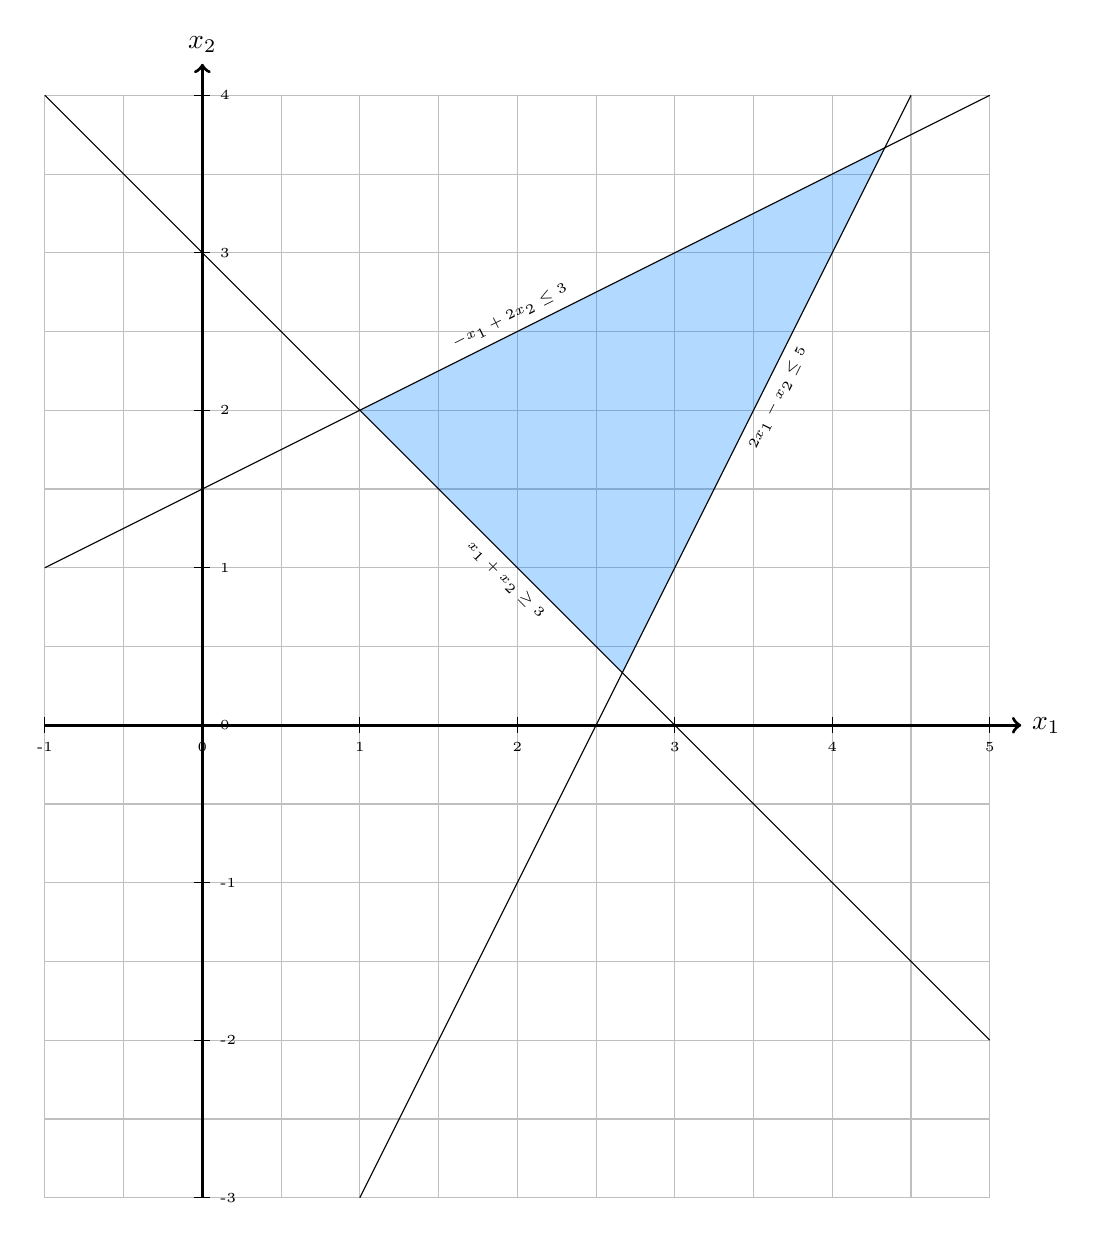
\begin{tikzpicture}[scale=2]
    \draw[gray!50, thin, step=0.5] (-1,-3) grid (5,4);
    \draw[very thick,->] (-1,0) -- (5.2,0) node[right] {$x_1$};
    \draw[very thick,->] (0,-3) -- (0,4.2) node[above] {$x_2$};

    \foreach \x in {-1,...,5} \draw (\x,0.05) -- (\x,-0.05) node[below] {\tiny\x};
    \foreach \y in {-3,...,4} \draw (-0.05,\y) -- (0.05,\y) node[right] {\tiny\y};

    \fill[blue!50!cyan,opacity=0.3] (8/3,1/3) -- (1,2) -- (13/3,11/3) -- cycle;

    \draw (-1,4) -- node[below,sloped] {\tiny$x_1+x_2\geq3$} (5,-2);
    \draw (1,-3) -- (3,1) -- node[below left,sloped] {\tiny$2x_1-x_2\leq5$} (4.5,4);
    \draw (-1,1) -- node[above,sloped] {\tiny$-x_1+2x_2\leq3$} (5,4);

	\end{tikzpicture}
	\end{center}
	Corresponding to the following system of inequalities:
	
	\begin{tcolorbox}[title=Remark,colframe=black,arc=10pt]
	Linear programming is widely used (to name only the most famous case) in Logistics (maximal flow problem also named "\NewTerm{transport problem}\index{transport problem}"), in corporate finance or also in decision theory when we solve a mixed strategy game (see the section of Game and Decision Theory  for a practical example). That's why Microsoft Excel 12.0 and earlier includes a tool named the "solver" in which there is an option named "Assume Linear Model" which then requires the use of the simplex model that we will study below:
	\begin{figure}[H]
		\centering
		\includegraphics{img/computing/excel_solver_lp.jpg}
	\end{figure}
	or since the 2010 version of the software (the user interface has completely changed):
	\begin{figure}[H]
		\centering
		\includegraphics[scale=0.8]{img/computing/excel_solver_lp_2010.jpg}
	\end{figure}
	\end{tcolorbox}
	We will focus in particular in the section on the most widely used algorithm for linear optimization named the "\NewTerm{simplex algorithm}\index{simplex algorithm}".
	
	When a problem can be modeled as an economic function to be maximized with respect to certain constraints that are purely additive, so are typically in the context of linear programming.
	
	So an economic function $Z$ as:
	
	where the $x_i$ are variables that affect the value of $Z$, and the $c_i$ the weights of these variables modeling the relative importance of each of them on the value of the economic function.
	
	The constraints  related to the variables are expressed by the following linear system:
	
	Under general and matrix form this problem is written as:
	
	
	To see the different method of resolution let us use an example as theoretical introduction:
	
	A factory produces two types of pieces $P1$ and $P2$ machined in two workshops $A1$ and $A2$. Machining times are for $P1$ or $3$ hours in the workshop $A1$ and $6$ hours in the workshop $A2$ and of for $4$ hours for $P2$ in the workshop $A1$ and $3$ hours in the workshop $A2$.
	
	Weekly up-time of human resources (workers) of the $A1$ workshop is $160$ hours and that of the workshop $A2$ is $180$ hours.
	
	The profit margin is of $1,200.-$ for the pieces $P1$ and $1,000.-$ for pieces $P2$.

	The question is how much of each kind of piece should we make to maximize weekly margin?
	
	This will be formalized as follows (canonical formulation):
	
	
	\paragraph{Graphical LP resolution}\mbox{}\\\\
	The graphical method is will adapted for problem with $2$ or $3$ variables but not more as our perception of hypervolume is quite limited for humans.
		
	When translate our optimization problem into graphical form, we speak also of "\NewTerm{polygon of constraints}\index{polygon of constraints}". Indeed, the economical constraints are represented by half planes. The solutions, if they exists, belongs to the intersection set name "\NewTerm{set of admissible solutions}\index{set of admissible solutions}" and is quite trivially represented in our case by:	
	\begin{figure}[H]
		\centering
		\includegraphics{img/computing/lp_graph.jpg}
		\caption{Illustration of a simple operational research problem with are of feasible solutions}
	\end{figure}
	\begin{tcolorbox}[title=Remark,colframe=black,arc=10pt]
	In the general case, for those who love the language of mathematicians ..., the information of a linear constraint geometrically corresponds to a half a space of $n$-dimensional space ($n$ being the number of variables) . In the elementary case, all the points in space that satisfy all constraints is limited by convex portions of hyperplane (see the case wiht $2$ variables, easy to illustrated), that is why the this is named also "\NewTerm{convex optimization}\index{convex optimization}". If the cost function is linear, the extreme point is a vertices (easy to see). The basic algorithm simplex algorithm (see further below) strat from one vertices and goes to the next vertices which locally maximizes the cost, and restarts the procedure as long as necessary.
	\end{tcolorbox}	
	To find the coordinates of the vertices, we can use the graph if the points are easy to determine.

	It is therefore to seek inside this area (connex), the pair  $(x_1,x_2)$ maximizing the economic function.

	However, the equation $Z$ is represented by a constant line of constant slope ($-1.2$) which all points $(x_1,x_2)$ provide the same $Z$ value for the objective function.
	
	In particular, the straight line $1200x_1+1000x_2$ pass trough the origin and it provides a zero value to the economic function. To increase the value of $Z$ and therefore of the economic function, we have to take away from the origin (in the quarter $x_1>geq 0,x_2\geq 0$ that is to say in the \texttt{I}st quadrant) the line of slope $-1.2$. Obviously then we see very quickly that the simplex method will not work if the constraints of the polygon does not contain the origin point!
	
	To meet the constraints, this straight line will be moved until the limit where it will not have a point of intersection anymore in comme with the are of admissible solutions (eventually a segment).
	\begin{figure}[H]
		\centering
		\includegraphics{img/computing/lp_graph_detailed.jpg}
		\caption{Finding solutions graphically with the economic function}
	\end{figure}
	The optimal solution is therefore necessarily located on the periphery of the region of admissible solutions and the parallel formed by translating the economic function are named "\NewTerm{isoquants lines}\index{isoquants lines}" or "\NewTerm{isocost lines}\index{isocost lines}"...
		
	\paragraph{Algebraic LP resolution}\mbox{}\\\\	
	Let us now see how to solve this problem analytically before moving to the theoretical part.
	
	So we have the "\NewTerm{canonical system}\index{canonical system}":
	
	with:
	
	We first introduce the "\NewTerm{slack variables}\index{slack variables}" to transform the $2$ inequalities in equalities. The system of equations takes then "\NewTerm{standard form}\index{standard form}":
	
	Therefore, for $x_1,x_2\geq 0$ fixed, the slack variable whose coefficients are always unit, measure the distance to travel to reach the vertices.

	It goes without saying that the technique of slack variables may be used for linear (or nonlinear) systems. Therefore, an constraint optimization system with inequalities, can always be reduced to an optimization system with equalities.
	\begin{tcolorbox}[title=Remark,colframe=black,arc=10pt]
	Obviously there is as much slack variable as inequalities.
	\end{tcolorbox}
	For the remaining part, we have noticed, after a review of this section, that the technique using tables (that we will see later) often presented in books and websites finally brought nothing to a deep understanding of the resolution mechanism (even if to program the computational method that is most convenient). Since the purpose of this book is to always prove with a maximum detail the operating principle of things so it goes without saying that we will opt for a first purely algebraic approach. Let us see it by returning to the system with the slack variables and the economic function but slightly rearranged:
	
	The $A1$ constraint then becomes:
	
	and the constraint $A2$ respectively becomes:
	
	Therefore, the problem consist to maximize $Z$ with the constraints:
	
	Let us start with an obvious feasible solution given the constraints that is trivially:
	
	Therefore with the system:
	
	we find immediately:
	
	The parameters in the actual state can be summarized as:
	
	To go forward, the goal will be to make $Z$ grow and for this purpose we will increase only one single variable, choosing the one with the largest coefficient (weight) in:
	
	that is to say $x_1$ (because implicitly we think this is how the $Z$ will increase the faster). We speak then of $x_1$ as the "\NewTerm{pivot direction}\index{pivot direction}". We keep then $x_2=0$ and we increase $x_1$ with the system which then reduces to:
	
	Therefore with $x_2=0$ and to begin $x_1=1$, we have:
	
	and we see that the constraints $x_1,x_2,x_3,x_4\geq 0$ are still respected, it is the same if $x_1$ is equal to $2$, $3$, $4$, $5$, ... and this until $31$, because after:
	
	and one of the slack variable has become negative, the constraints $x_1,x_2,x_3,x_4\geq 0$ are not all met and therefore this solution is not feasible.
	
	The question in the general case is to ask ourselves until what value (the most constraint value, verbatim the smallest) we can increase $x_1$ while maintaining the condition $x_1,x_2,x_3,x_4\geq 0$ when $x_2=0$? And the answer is quite simple:
	
	and therefore it is:
	
	then we speak sometimes of the "\NewTerm{pivot step}\index{pivot step}". We then have the actual solution:
	
	Which gives:
	
	Graphically, this is what we have just do:
	\begin{figure}[H]
		\centering
		\includegraphics{img/computing/lp_graph_detailed_with_pivot.jpg}
		\caption[]{Direction of the pivot head and arrival at point $(30, 0)$}
	\end{figure}
	To continue to increase $Z$ such simply (by increasing only one variable), we need a new system of equations similar to the original system:
	
	where we had expressed the variables that takes are non-zero value depending on others who take a zero value, that is to say $x_3,x_4$, in function of $x_1,x_2$ since we had for recall:
	
	For the remaining part, we must express $x_1,x_3$ and also $Z$ in function of $x_2,x_4$ since we just get for reminder:
	
	Before getting the new system reaction function, making some algebraic manipulations:
	
	which gives after simplification:
	
	and therefore it comes:
	
	which gives after simplification:
	
	and we have identically:
	
	So finally the system is:
	
	from which we reiterate the process (we increase only one  variable in $Z$ keeping the other to $0$). When we can not increase $Z$ as all coefficients are negative, well it is that we are at a maximum (thank you convexity...). Let us see this...
	
	In $Z$ the biggest coefficient is now $x_2$ and so it leads us to put $x_4=0$. The most constraint value of $x_2$ that allows to always respect the constraints $x_1,x_2,x_3,x_4\geq 0$ is therefore:
	
	And for this value, we have:
	
	The original economic function then takes the value:
	
	which therefore corresponds graphically to:
	\begin{figure}[H]
		\centering
		\includegraphics{img/computing/lp_graph_detailed_with_pivot_second_iteration.jpg}
		\caption{Pivot direction with arrival point at $(16, 28)$ for the second iteratio}
	\end{figure}
	So we see above that we arrived at the optimum value visible on the graph given at the beginning of this example. But how do we know that we arrived at the final point if we do not have plots or if we work in higher dimensions?
	
	In fact, the process is terminated either when all the coefficients of the economic function are negative or that the most constraignant value that respects the constraints is equal to zero !!! Let's see if this is the case! We therefore have in our example:
	
	So we'll rewrite the system:
	
	with this time $x_1,x_2$ and $Z$ dependant to $x_3,x_4$. We then have first:
	
	and we have:
	
	Therefore for $Z$ we have (the coefficients are all negative so we guess what comes ...):
	
	We then have the new system:
	
	As all coefficients of $Z$ are now negative, we're blocked because we would go in the wrong direction if we continue. We must therefore stop here and we adopt finally the solution:
	
	The method of resolution using tables that is often presented in the literature is only useful to write the coefficients of the variables of the system a table, but the changes that we made are exactly those we just made algebraically before (but a the opposite of the tables the method we used don't hide the logic of the method).
	
	\paragraph{Simplex algorithm LP resolution}\mbox{}\\\\
	To implement the  simplex algorithm, we must write the problem in a "standard" form and introduce the concept of "base program" that is the algebraic expression corresponding to the notion of "extreme point of the polyhedron of eligible programs" presented earlier above. Indeed, we will see that the solution of a problem of the linear programming type it exists, can still be obtained with a base program. The simplex method will therefore be to find a first base program and to build a following base programs constantly improving the economic function and thus leading to the optimum (this is what we name "dynamic programming").
	
	An LP problem is said to be placed in its "\NewTerm{standard form}\index{standard form}" if it involves the search for the minimum of the objective function, the latter being subject to constraints in the form of linear equations and conditions of non-negativity of the variables, that is, say we can write it in the form earlier before:
	
	That is to say, using matrix notation:
	
	where the matrices $C:n\times 1, A:m\times n,b:m \times 1$ respectively correspond to the activity coefficients of objective function, to the technical coefficients of activities and to second members of the constraints.

	We will now see how a LP general problem can always be reduced to a standard form. As we guess it the concept of "slack variable" will be essential to perform this "reduction".

	Find the maximum of a function $f (x)$ is equivalent to find the minimum of the opposite sign function $f (x)$. Moreover, a constraint which is presented as an inequality:
	
	can be replaced by the system:
	
	where as we already know $s_i$ is the slack variable constraint such that $s_i\geq 0$.
	
	Of course, if the system is such that:
	
	can be replaced by the system:
	
	implying again to add a slack variable  and always with the constraint that $e_i\geq 0$.

	This work of putting in standard form work us to find a system of linear equations to solve system (we saw previously at the beginning of this section how to solve this kind of system with the pivot algorithm).

	The matrix $A$ representing the components of the system of equations can be, as we know, expressed in different ways depending on the chosen vector basis (\SeeChapter{see section of Vector Calculus}). We will introduce now the concept of "\NewTerm{canonical associated usable form}\index{canonical associated usable form}" by choosing a special base and show that this reformulation of constraint system will enable us to move towards the optimum.
	
	The matrix $A$ can, after introduction of the slack variables be decomposed into two sub-matrices $[D|B]$, one containing the initial variables $D$ and the other with the slack variables $B$ such that:
	
	\begin{tcolorbox}[title=Remark,colframe=black,arc=10pt]
	The slack variables are variable and not constant!! In a system where the variables are in quantity $n$ and the equations in quantity $m$ to have as a system where one of the equation would be written:
	
	To add a slack variable such that:
	
	where $x_{n+1}=e_i$ on each row $m$, the added slack variable being different of all variables already existing in the system. This is why we can decompose the matrix in two submatrices..
	\end{tcolorbox}
	The columns of the matrix $B$ are obviously, by definition of the method, units columns, linearly independent. These columns form a basis of the vector space of columns of $m$ elements (or dimensions) - the number of  lines of the system. We name $B$ the "\NewTerm{base matrix}\index{base matrix}".
	
	Right now it can seem a little bit confusing. So let us continue the theorey with a companion example as we have for habit to do it in this book.
	The text below describing the simplex algorithm has been taken to Marcel Oliver (April 12, 2012) and formalized by our own work.
	\begin{enumerate}
	\item Step 1: Write the linear programming problem in standard form
	
	Turning a problem into standard form involves the following steps.
	\begin{enumerate}
		\item Turn Maximization into minimization and write inequalities in
		standard order.
		
		This step is obvious.  Multiply expressions, where appropriate, by
		$-1$.
		
		\item Introduce slack variables to turn inequality constraints
		into equality constraints with nonnegative unknowns.
		
		Any inequality of the form
		
		can be replaced by:
		  
		with $s \geq 0$.
		
		\item Replace variables which are not sign-constrained by differences.
		
		Any real number $x$ can be written as the difference of nonnegative
		numbers $x=u-v$ with $u,v\geq 0$.
	\end{enumerate}

	Consider the following example.
	
	subject to 
	
	Written in standard form, the problem becomes:
	
	subject to 
	

	\item Step 2: Write the coefficients of the problem into a
	"\NewTerm{simplex tableau}\index{simplex tableau}".
	
	The coefficients of the linear system are collected in an augmented
	matrix as known from Gaussian elimination for systems of linear
	equations; the coefficients of the objective function are written in a
	separate bottom row with a zero in the right hand column.
	
	For our example, the initial tableau reads:
	\newcolumntype{B}{%
	  >{\columncolor[gray]{.8}[.5\tabcolsep]}c}
	\begin{center}
	\begin{tabular}{BcccBBB|c}
	  $x_1$ & $x_2$ & $u$ & $v$ & $s_1$ & $s_2$ & $s_3$ \\
	  \hline
	  $1$ & $1$ & $-1$ & $1$ & $0$ & $0$ & $0$ & $1$ \\
	  $2$ & $-1$ & $-2$ & $2$ & $1$ & $0$ & $0$ & $5$ \\
	  $1$ & $-1$ & $0$ & $0$ & $0$ & $1$ & $0$ & $4$ \\
	  $0$ & $1$ & $1$ & $-1$ & $0$ & $0$ & $1$ & $5$ \\
	  \hline
	  $-1$ & $-2$ & $-3$ & $3$ & $0$ & $0$ & $0$ & $0$ 
	\end{tabular}
	\end{center}
	So following what we have above, we get for:
	
	that:
	
	The variables associated to the column components of the matrix $S$ will now be named "\NewTerm{bases variables}\index{bases variables}". In our case the bases variables are then essentially the slack variables that we will write now $x_{n+1},x_{n+2},\ldots,x_{n+m}$. The variables associates to the column of the matrix $X$ are named "\NewTerm{off-base variables}\index{off-base variables}", these are the variables $x_1,x_2,\ldots,x_n$.
	\begin{tcolorbox}[title=Remark,colframe=black,arc=10pt]
	Let us recall that in the expression of the economic function, only the off-base variables appear.
	\end{tcolorbox}
	In the following steps, we will act on the tableau by the rules of Gaussian elimination, where the pivots are always chosen from the columns corresponding to the bases variables.
	
	Before proceeding, we need to choose an initial set of basic variables
	which corresponds to a point in the feasible region of the linear
	programming problem.  Such a choice may be non-obvious, but we shall
	defer this discussion for now.  In our example, $x_1$ and $s_1, \dots,
	s_3$ shall be chosen as the initial bases variables, indicated by gray
	columns in the tableau above.
	
	\item Step 3: Gaussian elimination

	For a given set of basic variables, we use Gaussian elimination (\SeeChapter{see section Lineal Algebra}) to reduce the corresponding columns to a permutation of the identity matrix.  This amounts to solving $A\vec{x}=\vec{b}$ in such a way that the values of the nonbasic variables are zero and the values for the basic variables are explicitly given by the entries in the right hand column of the fully reduced matrix. In addition, we eliminate the 	coefficients of the objective function below each pivot.
	
	Our initial tableau is thus reduced to:
	\begin{center}
	\begin{tabular}{BcccBBB|c}
	  $x_1$ & $x_2$ & $\boldsymbol{u}$ & $v$ & $s_1$ & $s_2$ & $s_3$ \\
	  \hline
	  $1$ & $1$ & $\boldsymbol{-1}$ & $1$ & $0$ & $0$ & $0$ & $1$ \\
	  $0$ & $-3$ & $\boldsymbol{0}$ & $0$ & $1$ & $0$ & $0$ & $3$ \\
	  $\mathit 0$ & $\mathit{-2}$ & $\boldsymbol{\mathit{1}}$ & 
	    $\mathit{-1}$ & $\mathit 0$ & $\mathit 1$ & $\mathit 0$ & 
	    $\mathit{3}$ \\
	  $0$ & $1$ & $\boldsymbol{1}$ & $-1$ & $0$ & $0$ & $1$ & $5$ \\
	  \hline
	  $0$ & $-1$ & $\boldsymbol{-4}$ & $4$ & $0$ & $0$ & $0$ & $1$ 
	\end{tabular}
	\end{center}
	The solution expressed by the tableau is only admissible if all basic
	variables are non-negative, i.e., if the right hand column of the
	reduced tableau is free of negative entries.  This is the case in this
	example.  At the initial stage, however, negative entries may come up;
	this indicates that different initial basic variables should have been
	chosen.  At later stages in the process, the selection rules for the
	basic variables will guarantee that an initially feasible tableau will
	remain feasible throughout the process.

	\item Step 4: Choose new basic variables

	If, at this stage, the objective function row has at least one negative entry, the cost can be lowered by making the corresponding variable basic.  This new basic variable is named the "\NewTerm{entering variable}\index{entering variable}". Correspondingly, one formerly basic variable has then to become nonbasic, this variable is named the ""\NewTerm{leaving variable}\index{leaving variable}". We use the following standard selection rules.

	\begin{enumerate}
	\item The entering variable shall correspond to the column
	which has the most negative entry in the cost function row.  If all
	cost function coefficients are non-negative, the cost cannot be
	lowered and we have reached an optimum.  The algorithm then
	terminates.
	
	\item Once the entering variable is determined, the leaving
	variable shall be chosen as follows.  Compute for each row the ratio
	of its right hand coefficient to the corresponding coefficient in the
	entering variable column.  Select the row with the smallest finite
	positive ratio.  The leaving variable is then determined by the column
	which currently owns the pivot in this row.  If all coefficients in
	the entering variable column are non-positive, the cost can be lowered
	indefinitely, i.e., the linear programming problem does not have a
	finite solution.  The algorithm then also terminates.
	\end{enumerate}
	If entering and leaving variable can be found, go to Step~3 and
	iterate.
	
	Note that choosing the most negative coefficient in rule (i) is only a
	heuristic for choosing a direction of fast decrease of the objective
	function.  Rule (ii) ensures that the new set of basic variables
	remains feasible.  
	
	Let us see how this applies to our problem.  The previous tableau
	holds the most negative cost function coefficient in column $3$,
	thus $u$ shall be the entering variable (marked in boldface).  The
	smallest positive ratio of right hand column to entering variable
	column is in row $3$, as $\tfrac31<\tfrac51$.  The pivot in this row
	points to $s_2$ as the leaving variable.  Thus, after going through
	the Gaussian elimination once more, we arrive at
	\begin{center}
	\begin{tabular}{BcBcBcB|c}
	  $x_1$ & $\boldsymbol{x_2}$ & $u$ & $v$ & $s_1$ & $s_2$ & $s_3$ \\
	  \hline
	  $1$ & $\boldsymbol{-1}$ & $0$ & $0$ & $0$ & $1$ & $0$ & $4$ \\
	  $0$ & $\boldsymbol{-3}$ & $0$ & $0$ & $1$ & $0$ & $0$ & $3$ \\
	  $0$ & $\boldsymbol{-2}$ & $1$ & $-1$ & $0$ & $1$ & $0$ & $3$ \\
	  $\mathit{0}$ & $\boldsymbol{\mathit{3}}$ & $\mathit 0$ & $\mathit 0$ 
	      & $\mathit 0$ & $\mathit{-1}$ & $\mathit{1}$ & $\mathit 2$ \\
	  \hline
	  $0$ & $\boldsymbol{-9}$ & $0$ & $0$ & $0$ & $4$ & $0$ & $13$ 
	\end{tabular}
	\end{center}
	At this point, the new entering variable is $x_2$ corresponding to the
	only negative entry in the last row, the leaving variable is $s_3$.
	After Gaussian elimination, we find
	\begin{center}
	\begin{tabular}{BBBcBcc|c}
	  $x_1$ & $x_2$ & $u$ & $v$ & $s_1$ & $s_2$ & $s_3$ \\
	  \hline
	  $1$ & $0$ & $0$ & $0$ & $0$ & $\tfrac23$ & $\tfrac13$ & $\tfrac{14}3$ \\
	  $0$ & $0$ & $0$ & $0$ & $1$ & $-1$ & $1$ & $5$ \\
	  $0$ & $0$ & $1$ & $-1$ & $0$ & $\tfrac13$ & $\tfrac23$ & $\tfrac{13}3$ \\
	  $0$ & $1$ & $0$ & $0$ & $0$ & $-\tfrac13$ & $\tfrac13$ & $\tfrac23$ \\
	  \hline
	  $0$ & $0$ & $0$ & $0$ & $0$ & $1$ & $3$ & $19$ 
	\end{tabular}
	\end{center}
	Since there is no more negative entry in the last row, the cost cannot
	be lowered by choosing a different set of basic variables; the
	termination condition applies.

	\item Step 5: Read off the solution

	The solution represented by the final tableau has all nonbasic
	variables set to zero, while the values for the basic variables can be
	can be read off the right hand column.  The bottom right corner gives
	the negative of the objective function.
	
	In our example, the solution reads $x_1=\tfrac{14}3$, $x_2=\tfrac23$,
	$x_3=u=\tfrac{13}3$, $s_1=5$, $v=s_2=s_3=0$, which corresponds to
	$\zeta=-19$, which can be independently checked by plugging the
	solution back into the objective function.
	
	As a further check, we note that the solution must satisfy the initial equation and inequations.  This can obviously be checked by direct computation.
	\end{enumerate}
	In summary, any LP once put in standard form is such that:
	\begin{itemize}
		\item There is a square sub-matrix of matrix $A$, which is named the "base matrix" and is equal to the square unit matrix $\mathds{1}$ of size $m$ (indeed there are as many slack variables that lines in the original equations - at the number of $m$ - and as many columns as each slack variable has a different index).

		\item The basic variables involved does not appear in the expression of the economic function.

		\item The second member of the constraints consists of non-negative values.
	\end{itemize}
	We say then that the problem is put under a "a canonical form associated with the basis $B$, corresponding to the basis variables $x_{n+1},x_{n+2},\ldots,x_{n+m}$".
	
	\subsubsection{Nonlinear programming (Nonlinear optimization)}
	Nonlinear programming is the process of solving an optimization problem defined by a system of equalities and inequalities, collectively termed constraints, over a set of unknown real variables, along with an objective function to be maximized or minimized, where some of the constraints or the objective function are nonlinear. 
	
	A nonlinear optimization program (NLOP) is a generalization of linear programming (simplex algorithm) but about nonlinear functions and can also include nonlinear constraints and nonlinear economic functions.

	The purpose of what follows is to understand in outline but with an acceptable level of rigour the optimization tools that offer many spreadsheets softwares like the previous versions of Microsoft Excel to the version 2007 (since the version 2007 we cannot make a fine-tuning of these options anymore):
	\begin{figure}[H]
		\centering
		\includegraphics{img/computing/excel_solver_nonlinear_optimization.jpg}
		\caption{Microsoft Excel 2003 Solver Options}
	\end{figure}
	 We will especially see now in what consist the \textit{Newton} Search (meaning implicitly: "Gauss-Newton method") with the \textit{Tangent} and \textit{Quadratic} estimates. After which we will study also the Conjugate Gradients Search also with the tangent and quadratic methods respectively.
	 \begin{tcolorbox}[title=Remark,colframe=black,arc=10pt]
	We will stop at the study of the above cited models because there is an excessive quantity of empirical models such as for example the best known models (algorithms): substitution method, method of Lagrange multipliers, Nelder-Mead algorithm, Broyden-Fletcher-Goldfarb-Shanno (BFGS) algorithm, algorithm  of simultaneous annhiliation (SA), methods of interior points... and see Wikipedia for a more complete list (there are over a dozen of methods without taking into account the variations including empirical adjustments).
	\end{tcolorbox}
	We will see it further below, but we already guess that the choice \textit{Tangent} use a linear approximation (tangent) of the function to be optimized at the point considered when at the opposite the \textit{Quadratic} option will make an estimation of a function of the second degree at the considered point (typically a parabola). If at the considered point, the function is well modeled by a quadric, then the \textit{Quadratic} option can save time by choosing a better starting point that will require fewer steps on each additional research. If you have no idea of the behavior of a priori function, then the  \textit{Tangent} option is slower but safer.
	
	A well known example in the literature to introduce the search of optimums of nonlinear functions, before moving on to the part taking into account constraints on the system, is the "humpback whale function" of that consist to find the minimum of:
	
	With the range constraints:
	
	what we can indeed check visually:
	\begin{figure}[H]
		\centering
		\includegraphics{img/computing/humpback_whale_function.jpg}
		\caption{Plot of the humpback whale function with minima already visible}
	\end{figure}
	Either with Maple 4.00b:
	
	\texttt{>plot3d(x\string^2*(4-2.1*x\string^2+1/3*x\string^4)+x*y+y\string^2*(-4+4*y\string^2),\\
 x=-2..2,y=-1..1,contours=20,style=patchcontour,axes=boxed);}

	That gives:
	\begin{figure}[H]
		\centering
		\includegraphics[scale=0.65]{img/computing/humpback_whale_function_maple.jpg}
	\end{figure}

	As we can see, this function is a great example of multiple local minimum but there is also a must more vicious one that we will refer to when we will study evolutionary algorithms, the "Rastgrini's function":
	
	\texttt{>plot3d(20+x\string^2+y\string^2-10*(cos(2*Pi*x)+cos(2*Pi*y)),\\ 	x=-5..5,y=-5..5,contours=20,style=patch,axes=boxed,numpoints=10000);}
	
	That gives:
	\begin{figure}[H]
		\centering
		\includegraphics[scale=0.65]{img/computing/rastgrini_function_maple.jpg}
	\end{figure}
	
	\paragraph{Substitution Method}\mbox{}\\\\
	The least complex method for solving a non-linear programming problem is named the "\NewTerm{substitution method}\index{substitution method}".

	This method is restricted to models containing a single constraint and must be in addition to the equality type.

	Let us consider a companion example by considering the following economic function to maximize:
	
 	with the constraint (remember that it must be an equality !!!):
	
 	The first step is then to arbitrarily substitute:
	
 	In the economic function to get:
	
 	This therefore brings us back to a function to be maximized which is unconstrained, so we can differentiate it and put it as zero. Then it comes:
	
	that gives:
	
	From this we can deduce immediately that
	
 	By injecting those two values in the economic function, we then have:
	
	We see by this example very quickly the limitations of this technique. The first being that the economic function was not too complex, the final equation to solve was therefore not a problem, the second being that there were only two variables, the third being that the constraint must be an equality as we have already mentioned.
	
	
	\paragraph{Lagrange Multipliers Method}\mbox{}\\\\	
	The "\NewTerm{Lagrange multipliers method}\index{Lagrange multipliers method}" is a rather general technique for solving nonlinear programming problems with one or more constraints with linear or non linear economic function with inequalities (rather than strict equations only) and with more than two variables (for Other examples than those presented here the reader can go to the corresponding page of Wikipedia).

	We will begin to present this technique by a simple case which consists simply of taking again the example used during our study of the method of substitution:
	
	The first step is to write the constraint function in Lagrangian form as we do in Analytical Mechanics (\SeeChapter{see section  Analytical Mechanics}) at the difference that there are no general variables depending on the time:
	
	For this, we write first:
	
	Then the idea is that since this expression is null, nothing prevents us from summing it or subtracting it from the economic function with why not an empirical multiplier that we will denote $\lambda$ and which we will name the "\NewTerm{Lagrange multiplier}".

	It comes then if we choose to subtract for example (in fact the choice of the subtraction is made by anticipation of an interpretation of the Lagrange multiplier that we will see immediately after):
	
	Which gives us our Lagrangian function. In generic form the latter is often written as following:
	
 	Now the idea is to determine the values of the variables where the partial derivatives of the Lagrangian with respect to the variables vanish at the same time (corresponding in Analytichal Mechanis as the sum of all the Lagrangians relatively to one variable to be equal to zero):
	
 	What is generally written as:
	
	We therefore have a system of three equations with three unknowns which we know trivially how to solve (\SeeChapter{see section Linear Algebra}). We then get as solutions:
	
 	Notice that if we had not taken into consideration $\lambda$ and therefore that implicitly that latter had been equal to $1$ since the beginning, we would have had the following system of equations:
	
	and therefore we would not have obtained the results of the substitution method seen previously ... hence the multiplicative factor!

	The final value of $Z$ is then the same as for the substitution method taking into account $\lambda$!!!

	Although the Lagrange multiplier method is powerful, its increasing complexity with a large number of variables makes it a difficult tool to manipulate in practice.

	We will now focus on the interpretation of $\lambda$. As we shall see, the latter represents the local variation rate per unit of positive variation of the constant of the constraint function. Thus, if the constraint function becomes (we have changed the $40$ into a $41$):
	
	By doing again the same calculations as before, we then get
	
 	Therefore, by having increased of one unit the constant of the constrained function, we have:
	
 	In general, if the Lagrange multiplier is positive, then the economic function will increase if the constant of the constraint is also incremented positively and vice versa.

	Let us now consider a case much more elaborate a useful for our stud of Economics (especial Portfolio Optimization). We want to solve by the method of the Lagrange Multipliers the Markowitz portfolio problem (\SeeChapter{see section Economy}):
	
	with for recall:
	
	To facilitate the developments that will follow we will write this system with the following notation (for the details on the notations see the section Economy):
	
	The Lagrangian function will therefore be written:
	 
	Therefore:
	 
 	Now we calculate:
	 
	This gives us the system of three equations:
	  
	By rearranging the first equation:
	 
 	We have:
	 
 	Let us now take the two equations:
	
	Thus in an equivalent way:
	
	By injecting in it the explicit relation of the weights of the portfolio, we have:
	
	We can put this system in matrix form:
	
	Which gives us:
	
	Therefore:
	
	So once we have the values of these two Lagrange multipliers, we just have to inject them into:
	
 	To have weights that minimize the portfolio variance:
	
	So the reader will see during our study of Modern Portfolio management that getting the optimal weights is much more easy using the Lagrange multiplied method (and less time consuming) than using a software optimizer!
	\begin{tcolorbox}[title=Remark,colframe=black,arc=10pt]
	By the way the attentive reader will perhapse have noticed that finally making all the developement with the factor $1/2$ is useless since during the final substitution, the latter is neutralized with itself since $2$ is multiplied by $1/2$.
	\end{tcolorbox}
	
	\pagebreak
	\paragraph{Newton-Raphson Method (Quadratic Newton)}\mbox{}\\\\
	The "\NewTerm{Newton-Raphson method}\index{Newton-Raphson method}" is a technique for searching the extremum of a function or also, as we will see it when we will compare with a special example the difference between the Gauss-Newton method with that of Newton, for nonlinear regression.

	The Newton-Raphson, who in earlier versions to Microsoft Excel 2007 was activated in the solver by selecting Newton and Quadratic option uses the second order Taylor approximation (ie with second order derivatives) to have a quadratic function (parabola) which converges if the origin point of the research is close to the optimum. This approximation is repeated to each iteration.

	To start the formal approach let us recall that we have proved in the section Sequences and Series that a Taylor expansion for a function of two variables could be written in quadratic approximation by:
	
	where for recall $h$ and $k$ are variables and $x_0,y_0$ are fixed and where we have the Hessian matrix:
	
	that American experts in the field have a habit (unfortunate in my opinion ...) Note:
	
	the latter expression being the most common can be very misleading with the notation of the Laplacian.

	In the field of numerical methods it is customary to write the Taylor series above with few notations changes by putting first:
	
	This gives us a more condensed and technical form of the Taylor series around $\vec{x}$:
	
	By changing again a little bit the notations:
	
	We thus fall back on the usual expression of a function of $\mathbb{R}^2\rightarrow \mathbb{R}$ evaluated in Taylor series centered on $\vec{x}$.

	But if we seek for a local extrema (also sometimes named "\NewTerm{critical point}\index{critical point}"), we will need in first time that the derivative of the whole Taylor series be equal to zero. That is to say:
	
	and that the determinant of the Hessian matrix is positive (\SeeChapter{see section Sequences and Series}). And to know if we are on a local maximum or local minimum, we must look at the sign of $\partial_x^2 f(\vec{x})$.

	Let us rewrite the above relation explicitly as we proved it in the section of Sequences and Series for pedagogical reasons:
	
	And let us recall that all terms $x_0,y_0$ are constants because it is either the function $f$ evaluated the particular point $(x_0,y_0)$, or the partial derivative evaluated at the same point, either the partial second derivative always evaluated at the same point, etc.

	So finally the gradient will give:
	And let us recall that all terms $x_0,y_0$ are constants because it is either the function $f$ evaluated the particular point $(x_0,y_0)$, or the partial derivative evaluated at the same point, either the partial second derivative always evaluated at the same point, etc.

	So finally the gradient will give:
	
	and returning traditional notations in the field of numerical methods, we have then:
	
	And so as the gradient has to be equal zere, we have:
	
	and after a first rearrangement:
	
	and a second rearrangement:
	
	which often written:
	
	and by american specialists:
	
	Finally, before moving on to a concrete example it is important that the reader remembers the relation just seen above:
	
	
	\pagebreak
	\begin{tcolorbox}[colframe=black,colback=white,sharp corners]
	\textbf{{\Large \ding{45}}Example:}\\\\
	We are seeking a local extremum of the "humpback whale" function shown earlier above:
	
	with the starting point (arbitrary):
	
	To do the search, we calculate the gradient:
	
	and the hessian matrix:
	
	We then have:
	
	and:
	
	and:
	
	and therefore:
	
	and we start again (with less detail):
	
	\end{tcolorbox}
	
	\pagebreak
	\begin{tcolorbox}[colframe=black,colback=white,sharp corners]
	
	and therefore:
	
	and once again (with again less details):
	
	and therefore:
	
	and again (with even less detail):
	
	and values will not move anymore. But if we look at the original graphic where we highlighted the convergence point by a red point:
	\begin{figure}[H]
		\centering
		\includegraphics[scale=0.85]{img/computing/convergence_point_humpback_whale_example.jpg}
		\caption[]{Highlight of the convergence point in the humpback whale function}
	\end{figure}
	we see that this system does not search a a global extremum bu a local extremum as we already specified it. In fact, as the reader may test itself, convergence is very sensitive to initial starting point.
	\end{tcolorbox}
	
	\paragraph{Gauss-Newton Method (Tangent Newton)}\mbox{}\\\\
	The Gauss-Newton method is a powerful approximation without the derivatives of the second order of the Newton-Raphson method that in the prior versions of Microsoft Excel 2007 was activated in the solver by selecting the option \textit{Newton} and \textit{Tangent}.

	To study this method, let us do use a companion concrete example. Suppose we obtained the following data:
	
	and we suppose "a priori" that the data follow the following theoretical model (we could also try any other function):
	 
	We look then for $x_1,x_2$ that minimize the sum of squares between the experimental and theoretical values such that:
	
	with therefore:
	
	Let us write following the traditition in this field:
	
	We then have the following common notation:
	
	Now, imagine that we found a bipoint $(x_1,x_2)=(\vec{x})$ that gives this minimum and let us write it $(\vec{x}_{*})$ and without forgetting that it will remain a local minimum and with luck a global one...! 

	Let us consider a special case that we will name "\NewTerm{compatible solution}\index{compatible solution}" and define by the fact the the bi-point that minimize the sum of squares of errors is also such that for all $i$ we have:
	
	Therefore it is immediate that:
	
	Before going further, let us notice for example that for a component $j$ (which corresponds in our case to each variable of the a priori supposed theoretical function of our model):
	
	where the last condensed equality is many times far to be obvious morever as it makes usage of the gradient of a vector field (\SeeChapter{see section Vector Calculus}) that we see rarely in practice. The reader that should be destabilized can refer directly to the numerical example further below to makes thing more clear.

	So to continue... we deduce that:
	
	and the "compatible solution" brings us obviously to:
	
	Following the same step, we have:
	
	So finally we have the following tow relations:
	
	Given that for the "compatible solution" we have:
	
	it follows that in this case the second relation becomes:
	
	where $H$ is the hessian matrix (\SeeChapter{see section Sequences and Series}) what American practitionners write simply:
	
	So we can approximate in the case of the compatible solution, the hessian that contains derivatives of the second order by derivatives of the first order.

	So we have finally in this special case the two relations that are the pillar of the Gauss-Newton method:
	
	Now let us recall the basic relation of the Newton-Raphson method obtained earlier above:
	
	and for information, any mathematical technique (because they are many of them!) that simplifies the Hessian matrix to the right of equality becomes part of the family named "\NewTerm{quasi-Newton methods}\index{quasi-Newton methods}".
	
	Well the Gauss-Newton method that interest us here and is therefore one of the techniques of the family of the "quasi-Newton methods" consists simply in a first step in getting rid of the second derivatives of the Hessian of the Newton-Raphson method at the right of the equality thanks to the previously established relations such that (attention to remember the abuse of writing!):
	
	and in a second time rewrite the gradient on the left ot the equality thanks thanks to also to the previously established relation. Which gives us:
	
	The factor $2$ being not very aesthetic, almost all reference books optimize the problem with the following start relation:
	
	So by simply multiplying by a factor $1/2$ (which does not change the result) we have then:
		
	Let us recall again that a spreadsheet software like Microsoft Excel can not determine the derivatives it will calculate them using the numerical methods of right or centered derivatives as we have presented a earlier above.

	Now let us come back to our example of the beginning! So we have:
	
	We start with a bipoint that seems the closest to the desired solution:
	
	Then we have:
	
	and therefore we have:
	
	Then it comes:
	
	What we can therefore rewrite as:
	
	We also have by extension:
	
	Then we apply the relation proved earlier above:
	
	Therefore:
	
	After a minor simplification:
	
	Therefore:
	
	and therefore the next bipoint for the iteration will be:
	
	Which of corresponds well to the values of the first iteration:
	
	We will not do again explicitly also the other iterations. So this is what we get in the end:
	
	with therefore for local solution at the 4th iteration:
	
	With Maple 4.00b we get:
	
	\texttt{>with(plots):}\\
	\texttt{>points:=plot([[1,3.2939],[2,4.2699],[4,7.1749],[5,9.3008],[8,20.259] ],style=point,color=blue,symbol=circle):}\\
	\texttt{>plot\_GN:=plot(2.5411*exp(0.2595*x),x=0..8):}\\	
	\texttt{>display([pict1,pict2]);}
	
	\begin{figure}[H]
		\centering
		\includegraphics{img/computing/gauss_newton_example_plot.jpg}
		\caption[]{Points and our interpolated Gauss-Newton function}
	\end{figure}
		
	To close this subject let us do a comparison with the Newton-Raphson method for the first iteration using the same starting bipoint. Let us recall again that for this latter method, the iterations are based on the relation:
	
	and we will write the function as following for the Newton-Raphson method:
	
	and:
	
	Then we have:
	
	that becomes:
	
	Then we have:
	
	That becomes:
	
	Thus:
	
	Therefore:
	and therefore the next bipoint for the iteration will be:
	
	which corresponds obviously to the values of the first iteration:
	
	We will not do again explicitly also other iterations. So this is what it gives finally about our function to be minimized:
	
	So the Newton-Raphson method converges in this case slower than that of Gauss-Newton.
	
	\pagebreak

	\subsection{Resampling statistics}	
	Resampling statistics refers to the use of the observed data or of a data generating mechanism (such as a die) to produce new hypothetical samples (resamples) that mimic the underlying population, the results of which can then be analyzed. With numerous cross-disciplinary applications especially in the sub-disciplines of the life science, resampling methods are widely used since they are options when parametric approaches are difficult to employ or otherwise do not apply. 
	
       Resampled data is derived using a manual mechanism to simulate many pseudo-trials. These approaches were difficult to utilize prior to 1980s since these methods require many repetitions. With the incorporation of computers, the trials can be simulated in a few minutes and is why these methods have become widely used.  The methods that will be discussed are used to make many statistical inferences about the underlying population. The most practical use of resampling methods is to derive confidence intervals and test hypotheses. This is accomplished by drawing simulated samples from the data themselves (resamples) or from a reference distribution based on the data; afterwards, you are able to observe how the statistic of interest in these resamples behaves. Resampling approaches can be used to substitute for traditional statistical (formulaic) approaches or when a traditional approach is difficult to apply. These methods are widely used because their ease of use. They generally require minimal mathematical formulas, needing a small amount of mathematical (algebraic) knowledge. These methods are easy to understand and stray away from choosing an incorrect formula in your diagnostics.
      \begin{figure}[H]
		\centering
		\includegraphics[scale=0.7]{img/computing/random_sampling.jpg}
		\caption{Summary of resampling in different methods (source: ?)}
	\end{figure}
	
	\subsubsection{Monte Carlo Simulations}
	Monte Carlo methods (or Monte Carlo experiments) are a broad class of computational algorithms that rely on repeated random sampling to obtain numerical results. They are often used in physical and mathematical problems (finance, supply chain, decisioneering, quality, etc.) and are most useful as workaround when it is difficult or impossible to use other mathematical methods.
	
	It finds applications in various fields including the following examples:
	\begin{itemize}
		\item Problems related to the neutron bomb (or any other problem of  the same family)

		\item Calculations of integrals or various parameters of random variables (finance, insurance, risk, forecasting)
	
		\item Resolution of elliptic or parabolic equations

		\item Solving linear systems

		\item Optimization Problem Solving (operations research, project management, supply chain)

		\item Creation of statistical tests (Anderson-Darling, Kolmogorov, Levene, Brown-Forsythe, etc.)
	\end{itemize}
	Thus there are two types of problems that can be treated by the Monte Carlo probabilistic method:
	\begin{enumerate}
		\item  problems, which have a random behavior 

		\item deterministic problems, which do not have a random behavior
	\end{enumerate}
	
	About the probabilistic case, the idea is to observe the behavior of a series of random numbers that simulates how the real problem behaves and derive statistical solutions/conclusions. We then speak of "\NewTerm{Monte Carlo estimation}\index{Monte Carlo estimation}".

	In the deterministic case, the studied problem is completely defined and we cam in principle predict its evolution, but some parameters of the problem can be treated as if it were random variables (this is typically the case in "vector regression" technique in Economy). The deterministic problem them becomes probabilistic and still solvable numerically. We then speak of "\NewTerm{Monte Carlo elaborated estimation}\index{Monte Carlo elaborated estimation}".
	
	Let us begin with the most used one in business: generating draws from a probability distribution. For this purpose we need to introduce the Inverse transform sampling.
	
	\begin{tcolorbox}[title=Remark,colframe=black,arc=10pt]
	The name of "Monte Carlo method" date around 1944. Isolated researchers have used however long before similar statistical methods: for example, Edwin Herbert Hall for the experimental determination of the speed of light (1873), or Kelvin in a discussion of the Boltzmann equation (1901), but the real use of Monte Carlo methods began with research on the atomic bomb.\\

	During the immediate postwar period, John Von Neumann, Encrio Fermi and Stanislaw Ulam warned the scientific community of the applicability of the Monte Carlo methods (eg for the approximation of the eigenvalues of the Schrödinger equation). The systematic study was made by Harris and Herman Khan in 1948. After an eclipse caused by too intensive use during the 1950s, the Monte Carlo method is back since almost everybody can run complex management or business strategic simulations on office computers (with softwres like @Risk or CrystalBall).  in short, wherever it is profitable to use simulation processes.
	\end{tcolorbox}
	
	\pagebreak
	\paragraph{Inverse Transform Sampling}\mbox{}\\\\
	Inverse transform sampling (also known as inversion sampling,  inverse probability integral transform, inverse transformation method, Smirnov transform, golden rule,) is a basic method for pseudo-random number sampling, i.e. for generating sample numbers at random from any probability distribution given its cumulative distribution function.
	
	Inverse transformation sampling takes uniform samples of a number $\mathcal{U}$ between $0$ and $1$, interpreted as a probability, and then return the largest number $x$ from the domain of the distribution $P(X)$ such that $P(-\infty < X < x) \le \mathcal{U}$. 
	
	Computationally, this method involves computing the quantile function of the distribution — in other words, computing the cumulative distribution function (CDF) of the distribution (which maps a number in the domain to a probability between $0$ and $1$) and then inverting that function.
	
	To use this we method we go through he "\NewTerm{probability integral transform}\index{probability integral transform}" that states that if $X$ is a continuous random variable with cumulative distribution function $F_X$, then the random variable $Y=F_X(X)$ has a uniform distribution on $[0, 1]$. The inverse probability integral transform is just the inverse of this: specifically, if $Y$ has a uniform distribution on $[0, 1]$ and if $X$ has a cumulative distribution $F_X$, then the random variable $F_X^{-1}(Y)$ has the same distribution as $X$.
	\begin{theorem}
	Suppose that a random variable $X$ has a distribution for which the cumulative distribution function (CDF) is $F_X$. Then the random variable $Y$ defined as:
	
	has a uniform distribution.
	\end{theorem}
	\begin{dem}
	Given any random variable $X$, define $Y = F_X (X)$. Then (it is not always easy to read this proof through the first time even if afterwards it is obvious):
	
	$F_Y$ is just the CDF of uniform random variable $\mathcal{U}[0,1]$. Thus, $Y$ has a uniform distribution on the interval $[0, 1]$.
	\begin{flushright}
		$\square$  Q.E.D.
	\end{flushright}
	\end{dem}
	The problem that the inverse transform sampling method solves is as follows:
	\begin{itemize}
		\item Let $X$ be a random variable whose distribution can be described by the cumulative distribution function $F_X$.
		\item We want to generate values of $X$ which are distributed according to this distribution.
	\end{itemize}
The inverse transform sampling method works as follows:
	\begin{enumerate}
		\item Generate a random number $\mathcal{U}$ from the standard uniform distribution in the interval $[0,1]$.
		\item Compute the value $x$ such that $F_X(x) =\mathcal{U}$ (using $F_X^{-1}(\mathcal{U})$).
		\item Take $x$ to be the random number drawn from the distribution described by $F_X$.
	\end{enumerate}
Expressed differently, given a continuous uniform variable $\mathcal{U})$ in $[0, 1]$ and an invertible cumulative distribution function $F_X$, the random variable $X = F_X^{-1}(\mathcal{U})$ has distribution $F_X$ (or, $X$ is distributed $F_X$).

	\pagebreak
	\paragraph{Random number generation}\mbox{}\\\\
	The best way to understand the method of Monte Carlo is to make examples (even small one should be enough). But for this, we must first have a good random number generator (which is quite difficult depending on the job). This is a very delicate and sensitive field for which an international standards is published (ISO 28640:2010 \textit{Random variate generation methods}).
	
	A random-number generator (RNG) is a computational or physical device designed to generate a sequence of numbers or symbols that cannot be reasonably predicted better than by a random chance.
	
	Several computational methods for random-number generation exist. Many fall short of the goal of true randomness, although they may meet, with varying success, some of the statistical tests for randomness intended to measure how unpredictable their results are.
	
	There are two principal methods used to generate random numbers. The first method measures some physical phenomenon that is expected to be random and then compensates for possible biases in the measurement process. Example sources include measuring atmospheric noise, thermal noise, and other external electromagnetic and quantum phenomena. For example, cosmic background radiation or radioactive decay as measured over short timescales represent sources of natural entropy.
	
	The second method uses computational algorithms that can produce long sequences of apparently random results, which are in fact completely determined by a shorter initial value, known as a seed value or key. As a result, the entire seemingly random sequence can be reproduced if the seed value is known. This type of random number generator is often named a "pseudorandom number generator". This type of generator typically does not rely on sources of naturally occurring entropy, though it may be periodically seeded by natural sources. This generator type is non-blocking, so they are not rate-limited by an external event, making large bulk reads a possibility.
	
	Let us take, to begin, an example with the Maple 4.00b random generator:
	\begin{figure}[H]
		\centering
		\includegraphics{img/computing/maple_random_generator.jpg}
		\caption{Pseudo-random generator with Maple 4.00b}
	\end{figure}
	and:
	\begin{figure}[H]
		\centering
		\includegraphics{img/computing/maple_random_generator_restart.jpg}
		\caption[]{Pseudo-random generator restart with Maple 4.00b}
	\end{figure}
	So we see that the default random number generator used by default in Maple 4.00b should be used with extreme caution since a system reset is enough to find... equal random values! This is therefore as we already said "\NewTerm{pseudo-random generator}\index{pseudo-random generator}" that gives possibilities to makes  sometimes named "\NewTerm{pseudo Monte Carlo method}\index{pseudo Monte Carlo method}".
	\begin{figure}[H]
		\centering
		\includegraphics{img/computing/maple_random_generator_special_library.jpg}
		\caption[]{Pseudo-random library with Maple 4.00b}
	\end{figure}
	The \texttt{RAND( )} and \texttt{RANDBETWEEN( )} functions of the of Microsoft Excel 14.0.6123 are also pseudo-random generators which here is a sample of 100 simulations (of course in Microsoft Excel the chart below will change each time you press on the keyboard button: F9):
	\begin{figure}[H]
		\centering
		\includegraphics{img/computing/random_generator_plot_excel.jpg}
		\caption[]{Illustration of a sequence of pseudo-random numbers with Microsoft Excel 14.0.6123}
	\end{figure}
	Unfortunately, it may happen with pseudo-random numbers that the numbers generated are presented in bunches, that is to say by sets of numbers close to each other, which reduces the effectiveness of the Monte Carlo simulation .

	An empirical technique is to use then sequences of numbers generated by algorithms that scan almost surely the range $[0,1]$. We speak then of "\NewTerm{quasi-random numbers}\index{quasi-random numbers}" to make simulations sometimes named "\NewTerm{quasi-Monte Carlo}\index{quasi-Monte Carlo}". In almost all Microsoft Excel, you can create a Visual Basic Application function that will replace the pseudo-random generators that are the \texttt{RAND( )} or \texttt{RANDBETWEEN( )}.

	Here is an example of such a V.B.A. function which generates quasi-random number named "\NewTerm{Fauré random number sequence}\index{Fauré random number sequence}":
	
	\begin{lstlisting}[language={[Visual]Basic}, caption={VBA Fauré sequence code}]
		Function SequenceFaure(n) As Double
    		Dim f As Double, sb As Double
    		Dim i As Integer, n1 As Integer, n2 As Integer
    
    		n1 = n
    		sb = 1 / 2
    		Do While n1 > 0
		        n2 = Int(n1 / 2)
		        i = n1 - n2 * 2
		        f = f + sb * i
		        sb = sb / 2
		        n1 = n2
		    Loop
		    SequenceFaure = f
		End Function
	\end{lstlisting}
	This will gives the following sequence for a sample of $100$ simulations:
	\begin{figure}[H]
		\centering
		\includegraphics{img/computing/faure_pseudo_random_sequence_excel.jpg}
		\caption[]{Illustration of a Fauré sequence of pseudo-random numbers with Microsoft Excel 14.0.6123}
	\end{figure}
	where we see well that the sequence covers well the whole area between $0$ and $1$ (we say then that: it covers faster the integration surface). This technique is sometimes preferred because it has the advantage of keeping the values off the simulation every time we restart the simulation (therefore in Microsoft Excel the chart above will not change when you press the keyboard button F9) .

	By conse the sequence generators have a great weakness: they are only applicable (to my knowledge at least) for problems of simulations with a single random variable (typically pricing single option strategy following Black \& Scholes model). Indeed if we have several random variables (and this is the most common case!), then the variables are artificially correlated (correlation coefficient = $1$) because they travel all the area between $0$ and $1$ in the same way! So a good simulation with several variables is a simulation including the treated variables have a correlation coefficient which approaches zero!!!!!!

	In addition, sequence generators require algorithms that are very time consuming when there are many variables relatively to a pseudo-random generator, this is why in most situations we prefer the old methods.
	\begin{tcolorbox}[title=Remark,colframe=black,arc=10pt]
	As we already mention it, engineers should refer to the international standard ISO 28640: 2010 when they need to implement random number generators in their softwares.
	\end{tcolorbox}
	Once the pseudo-random or random generator created and tested, we can see some applicaton of the Monte Carlo method before continuing on performance tricks relatively to this method. Thus, in the calculation of integrals, this method is very useful and very fast in terms of convergence speed.
	
	\pagebreak
	\paragraph{Monte Carlo integration}\mbox{}\\\\
	In numerical integration, methods such as the Trapezoidal rule use a deterministic approach as we already know. Monte Carlo integration, on the other hand, employs a non-deterministic approaches: each realization provides a different outcome. In Monte Carlo, the final outcome is an approximation of the correct value with respective error bars, and the correct value is within those error bars.
	
	Consider for example the calculation of the following univariate defined integral of a function $f$ and positive over the interval $[a, b]$:
	
	Given:
	
	the maximal value of the function $f$ between the bounds $[a,b]$.

	We consider the rectangle bounding function on the interval $[a, b]$ defined by vertices $\{(a,0),(b,0),(b,m),(a,m)\}$:
	\begin{figure}[H]
		\centering
		\includegraphics{img/computing/monte_carlo_onedimensional_integration.jpg}
		\caption{Basic principle of the univariate integral calculation with Monte Carlo}
	\end{figure}
	We draw a large number $N$ of random points in this rectangle. For each point, we test if it is below the blue curve. Given $P$ the proportion of points below this curve, we have:
	
	The corresponding Maple 4.00b algorithm  is given by:\\
	
	\texttt{>intmonte:=proc(f,a,b,N)}\\
	\texttt{local i,al,bl,m,P,aleaabs,aleaord,isabove;}\\
	\texttt{m:=round(max(a,b)*10\string^4);}\\
	\texttt{al:=round(a*10\string^4);}\\
	\texttt{bl:=round(b*10\string^4);}\\
	\texttt{aleaabs:=rand(al..bl);}\\
	\texttt{aleaord:=rand(0..m);}\\
	\texttt{P:=0;}\\
	\texttt{for i from 1 to N do}\\
	\texttt{     isabove:=(f(aleaabs()/10\string^4)-aleaord()/10\string^4)>=0;}\\
	\texttt{     if isabove then}\\
	\texttt{          P:=P+1;}\\
	\texttt{     fi}\\
	\texttt{od:}\\
	\texttt{RETURN((b-a)*max(a,b)*P/N)}\\
	\texttt{end:}\\
	
	To call this procedure in Maple, just write \texttt{>intmonte(f, a, b, N)} but replacing the first argument passed as a parameter with the expression of a function and the other arguments by numerical values (obviously!).
	
	\paragraph{Monte Carlo Estimation of Pi}\mbox{}\\\\
	For the calculation of $\pi$ the principle is the same and therefore consist to use the proportion of the number of points in a quarter of circle area (this simplifies the algorithm by restricting the calculations to strictly positive coordinates) inscribed in a square of side $1$ (so the radius of the circle is also equal to $1$ obviously) relatively to the total number of points (to test if a point is outside the circle, we obviously use the Pythagorean theorem) such that:
	
	\begin{figure}[H]
		\centering
		\includegraphics{img/computing/monte_carlo_pi.jpg}
		\caption{Monte Carlo $pi$ estimate}
	\end{figure}
	The corresponding Maple 4.00b algorithm is given by:\\

	\texttt{>isinside:=proc(x,y) x\string^2+y\string^2<1 end:}\\
	\texttt{>calculatepi:=proc(N)}\\
	\texttt{local i,P,abs,ord,alea;}\\
	\texttt{alea:=rand(-10\string^4..10\string^4);}\\
	\texttt{P:=0;}\\
	\texttt{for i from 1 to N do}\\
	\texttt{     abs:=alea()/10\string^4;ord:=alea()/10\string^4;}\\
	\texttt{       if isinside(abs,ord) then}\\
	\texttt{            P:=P+1;}\\
	\texttt{       fi}\\
	\texttt{od;}\\
	\texttt{RETURN(4*P/N)}\\
	\texttt{end:}\\
	\texttt{>evalf(calculatepi(100));evalf(calculatepi(1000));\\evalf(calculatepi(10000));evalf(calculatepi(100000));}\\
	
	
	
	In terms of convergence it looks typically as:
	\begin{figure}[H]
		\centering
		\includegraphics{img/computing/monte_carlo_pi_convergence.jpg}
	\end{figure}
	
	\paragraph{Monte Carlo Modeling}\mbox{}\\\\
	The most common application of the Monte Carlo method in business and industry is certainly the study of random variables. Furthermore, this method is part of the ISO 31010 Risk Management standard under the name of "\NewTerm{Monte Carlo analysis}\index{Monte Carlo analysis}". Many cutting edge tech companies make Monte Carlo modeling with a spreadsheet softwares like Microsoft Excel (even multinationals!) and with a lesser extent with professional oriented softwares or add-ins such as @RISK, CrystalBall, TreeAge, Isograph or MATLAB.
	
	The advantages of this method in modeling random variables are:
	\begin{itemize}
		\item We can integrate any distribution  including empirical one and not continuous one!

		\item Models are very easy to implement and can be expanded as needed without too much effort.

		\item All influences or relation occurring in reality (at least the identified one....) may be represented and implemented in the model.

		\item Sensitivity analysis (\SeeChapter{see section Quantitative Management Techniques}) can be applied.

		\item The models are easily understable and provide a measure of the accuracy of the result.

		\item Many inexpensive software are available (at least inexpensive in comparison to criticality of the business analyzed that is most of time in the order of the billion of dollars).
	\end{itemize}
	Let us consider a simple but concrete case (widely used in business) that I like to use in my introduction training of a small project of two tasks denoted by $A$ and $B$ which follow each other without free margin (or free slack). Let us imagine that the duration of each task has been estimated in accordance with the recommendation of the Project Management Institute with a beta distribution (\SeeChapter{see section Statistics}) as learn it all project managers in their training curriculum (\SeeChapter{see section Quantitative Management Techniques}).

	For this example, the task $A$ has an optimistic duration of $5$ days and a pessimistic duration of $8$ days. Task $B$ an optimistic duration of $1$ day and a pessimistic duration of $4$ days. We would like in the spreadsheet software Microsoft Excel using a pseudo Monte Carlo simulation (therefore necessarily based on a pseudo-random variable) introduce three traditional minimum information:
	\begin{figure}[H]
		\centering
		\includegraphics{img/computing/monte_carlo_tasks.jpg}
	\end{figure}
	\begin{itemize}
		\item A table with $3$ columns (duration of $A$, $B$ and sum of both) and $10,000$ simulations (rows)
	
		\item The graphical distribution function of the sum of the two random variables 

		\item The convergence of the 95th percentile on the $100$ first simulations (useful for the subject further below).
	\end{itemize}
	We then construct the following table of $10,000$ row (the screenshot shows only the first rows...):

	where all cells from row $2$ to row $10,000$ of column A contains the following function (Microsoft Excel 14.0.7166):

	\begin{center}
	\texttt{=BETA.INV(RAND(),3+SQRT(2),3-SQRT(2),5,8)}
	\end{center}

	and for column B contains the following function:

	\begin{center}
	\texttt{=BETA.INV(RAND(),3+SQRT(2),3-SQRT(2),1,4)}
	\end{center}

	and finally the cell C1 contains the following function that was pull down until cell C10000:
	
	\begin{center}
	\texttt{=A2+B}
	\end{center}
	
	Obviously the values in Microsoft Excel 14.0.6123 will change each time you press the \texttt{F9} key on the keyboard.

	Then this gives us the histogram still made with the same software version (we will not detail how to building such a chart it is a basic subject of Microsoft Office knowledge and has nothing to do in a scientific book) where the $x$-axes are the number of days:
	\begin{figure}[H]
		\centering
		\includegraphics{img/computing/monte_carlo_histogram_tasks.jpg}
	\end{figure}
	and the convergence of the $95$th percentile of the first $100$ simulations (because as this example is simple, the system converges quickly enough so that we do not to need to take more than $100$ simulations as example) where the $y$-axes is the number of days:
	\begin{figure}[H]
		\centering
		\includegraphics{img/computing/monte_carlo_convergence_tasks.jpg}
	\end{figure}
	Obviously by default, in Microsoft Excel 14.0.6123 the chart above will change each time you pres the \texttt{F9} key on the keyboard.
	\begin{tcolorbox}[title=Remark,colframe=black,arc=10pt]
	In the case of the simulations of random variables, we can in simple cases involving only sums or subtractions of random variables, as is the case for the example above, determine the mean and the standard deviation of the results analytically using the property of linearity of the mean and variance (because normally for the variance of two independent random variables, the covariance is zero). By analyzing the difference between the analytical value and that obtained by numerical simulation, the offset can be corrected certain other statistical indicators by simply adding or subtracting the differential. This is known as the technique of "\NewTerm{control variables}\index{control variables}" that we will detail further below.
	\end{tcolorbox}
	There are other variance reduction techniques (ie: the standard deviation) that control variables technique Carlo to reduce the variance of the Monte Carlo estimators in specific conditions:

	\begin{itemize}
		\item One of these techniques is the use of "\NewTerm{antithetic variables}\index{antithetic variables}" which consists very simply (programming this technique at the high school level as you can see in the MATLAB™ companion book) to decorrelate simulations to make the covariance between the variables negative  and so reduce the global variance (such as we have seen in the section Statistics, the variance of the sum of two random variables make appear a covariance term). Unfortunately, this technique works satisfactorily with symmetric distributions this is why to my knowledge it is not implemented in simulation software available on the market.

		\item There are also the technique named "\NewTerm{stratified sampling}\index{stratified sampling}" that consist to cut the  pre-image space of the random variable in regular intervals (the programming of this technique is also at the high school level as you can see in the MATLAB™ companion book). This technique works very well when the number of simulations must be small but only in the case of a single variable. This also why, as far as we I know, it is not implemented in simulation softwares available on the market.

		\item There exist is a generalization of stratified sampling (the programming of this technique is also at the high school level) for simulations with multiple variables and that is named "\NewTerm{Latin Hypercube}\index{Latin Hypercube}" (abbreviated as "LHS" for Latin Hypercube Stratification). This technique ensures that each $n$-tuple of random variables (corresponding to a space of $n$ dimensions) uses a unique pre-image at each iteration, hence the name of that technique (Latin: refers to magic squares where each value appears uniquely, Hypercube because is an $n$-dimensional generalization of a magic square). Some simulation software available on the market implement this technique (@RISK, CrystalBall).
	\end{itemize}
	To summarize, whether that its the technique of Faure sequence generators, of antithetic variables, of control variables, of stratified sampling or Latin Hypercube even if these techniques are all easy to program, the method using the pseudo-random variables is privileged because is the most suitable for the majority of common situations in the business and in non-cutting edge scientific applications.
	
	\subsubsection{Bootstrapping}
	In statistics, "\NewTerm{bootstrap techniques}\index{bootstrap techniques}" can refer to any test or metric that relies on random sampling with replacement of a population of data to run statistical inference on small samples. This methods is relatively intensive in computations still for expensive office computers at this beginning of the 21st century.  
	\begin{figure}[H]
		\centering
		\includegraphics{img/computing/bootstrap_sampling.jpg}
	\end{figure}
	The goal of bootstrapping is to find some indication of a statistic: its estimate of course, but also its dispersion (variance, standard deviation), confidence intervals or hypothesis testing. This method is based on simulations, such as Monte Carlo methods, with the difference that the bootstrap does not require additional information than that that is available already in the initial sample. In general, it is based on new samples obtained by sampling with replacement from the original sample (then we speak also of "\NewTerm{resampling}\index{resampling}").
	
	We distinguish generally two types of bootstrap:
	\begin{enumerate}
		\item The bootstraps which make no assumptions about the probability distribution of the data analyzed. We then speak then as in statistics of "\NewTerm{non-parametric bootstrap}\index{non-parametric bootstrap}".

		\item The bootstraps replacing each data measured by those corresponding to the analytical expression of the law of probability distribution assumed. We speak then of "\NewTerm{parametric bootstrap}\index{parametric bootstrap}". Once all the original values replaced, the process is exactly that of the non-parametric bootstrap.
	\end{enumerate}
	We will illustrate the principle of the bootstrap on the example of the confidence interval of the mean $\mu$ of a random variable. For this example, the confidence interval for the mean of a random variable is completely determined from the mean and the variance calculated on the sample (\SeeChapter{see section Statistics}).

	We consider a sample of the random variable composed of $10$ estimates:
	
	La arithematic average of this sample is:
	
	and it standard deviation (maximum unbiased likelihood estimator of the standard deviation):
	 
	As we are in the situation of a known sample mean and a known sample variance, to do the calculation of a confidence interval, then we have proved in the section Statistics that we had to use:
	
	where $S$ is for recall another traditional notation in some areas of statistics for the notation of the empirical standard deviation (\SeeChapter{see section Statistics}). We then have for the confidence interval at $95\%$ of the mean:
		
	Therefore:
		
	Which gives:
	
	The confidence interval can also be calculated by bootstrap (this is especially useful for complicate distribution that are not symmetric and when we focus on the median rather than on the mean). Then it is therefor obtained by the Following algorithm:
	\begin{enumerate}
		\item From the initial sample, we simulate new samples of the same size, named "\NewTerm{bootstrap replicates}\index{bootstrap replicates}" of size $n$, by random draws with replacement (see figure above). For example with the previous series, we could get the following replicate:
		
		in which, by definition, some of the original sample values do not appear, and where others appear several times (yes it's a sampling with replacement therefore...). Several samples are simulated in this way. Se e can form a number of replicas (arrangements with replacement) equal to (\SeeChapter{see section Probabilities}):
		
		Therefore with $10$ values we have $10,000,000,000$ possibilities...
		
		\item For each simulated sample, an average\footnote{in fact the process is the same for any estimate of any statistical indicator $\hat{\theta}$} is calculated (so we will have several thousand of averages!). 
	
		\item The $95\%$ confidence interval is the calculate on this set of averages (or any other estimator) by typically using the percentile calculation (through the functions of a spreadsheet software or a programming/scripting language). This grouping is named the "\NewTerm{bagging}\index{bagging}" that is the abbreviation for "\NewTerm{Bootstrap Aggregating}\index{Bootstrap Aggregating}".
	\end{enumerate}
	Obviously for each set of bootstrap, the percentiles themselves will not be the same so it is even possible to create a confidence interval for the percentiles themselves!
	
	It is quite easy (just like the Monte Carlo methods) to create replicas with spreadsheet software like Microsoft Excel (at least for people that know a little bit how to use a spreadsheet software) without computer programming or scripting (see below an example with Microsoft Excel)! Furthermore, the bootstrap technique is very powerful because it does not use any assumptions about the underlying statistical distribution. 

	The most common field of application of bootstrapping in "direct" business (I don't mind about Data Mining for Marketing that is not what I mean about "direct business") that I know is in project management during meetings where a dozen people estimates the duration of a project task or project phase.
	
	Bootstrapping can therefore be applied to any estimator other than the average, as the median, the correlation coefficient between two random variables or the principal eigenvalue of a variance-covariance matrix (for principal component analysis), or the slope and intercept of a regression and this is its great strength!!! Indeed, for these estimators, there is no general mathematical relations that defines the standard error or confidence interval. The only methods applicable are resampling methods to which bootstrapping belongs to and this is intensively used since almost any home or office computer at the beginning of the 21st century is powerful enough to bootstrap small databases.
	\begin{tcolorbox}[colframe=black,colback=white,sharp corners]
	\textbf{{\Large \ding{45}}Example:}\\\\
	As example let us first use a spreadsheet software like Microsoft Excel table 14.0.6123 and taking the theoretical companion example above as practical software example (we prohibit ourselves of doing VBA programming). We then build a small table with the previous sample:
	\begin{figure}[H]
		\centering
		\includegraphics{img/computing/boostrapping_excel_initial_dataset.jpg}
	\end{figure}
	At the opposite of the companion theoretical example  would be able to determine a confidence interval for the median instead as for the arithmetic mean (we purposely take a statistical indicator for which there is simple analytical confidence interval). For this, we calculate the median of several thousand of replications in the column F (random choice!), where each replication corresponds to a row :
	\begin{figure}[H]
		\centering
		\includegraphics[scale=0.8]{img/computing/boostrapping_excel_resampling_median.jpg}
	\end{figure}
	\end{tcolorbox}
	
	\begin{tcolorbox}[colframe=black,colback=white,sharp corners]
	with the following quite long forula for Microsoft Excel Next 14.0.6123 to put in cell F5 and then pull down to the end of the sheet:\\
	
	\texttt{=MEDIAN(INDEX($A$5:$A$14,RANDBETWEEN(1,10),1),\\
INDEX($A$5:$A$14,RANDBETWEEN(1,10),1),\\
INDEX($A$5:$A$14,RANDBETWEEN(1,10),1),\\
INDEX($A$5:$A$14,RANDBETWEEN(1,10),1),\\
INDEX($A$5:$A$14,RANDBETWEEN(1,10),1),\\
INDEX($A$5:$A$14,RANDBETWEEN(1,10),1),\\
INDEX($A$5:$A$14,RANDBETWEEN(1,10),1),\\
INDEX($A$5:$A$14,RANDBETWEEN(1,10),1),\\
INDEX($A$5:$A$14,RANDBETWEEN(1,10),1),\\
INDEX($A$5:$A$14,RANDBETWEEN(1,10),1))
	}
	
	So we can not have more that 10 billion more... corresponding to the $\bar{A}_n^n$ calculate above (Microsoft Excel 14.0.6123 and after is limited  to $17,179,869,184$ cells...).\\
	
	Then simply in a cell of your choice we write:\\
	\begin{center}
	\texttt{=PERCENTILE(F5:F2003,0.025)}
	\end{center}
	and in another cell:\\
	\begin{center}
	\texttt{=PERCENTILE(F5:F2003,0.975)}
	\end{center}
	
	which will give will $2,000$ replication respectively $7$ and $29.5$.\\

	With basic knowledge of a spreadsheet software, it is possible to graphically show the convergence of the median in function the number of replications (below we used only the first $100$ replications):
	\begin{figure}[H]
		\centering
		\includegraphics[scale=0.7]{img/computing/boostrapping_excel_median_convergence.jpg}
		\caption[]{Convergence of the median in function of the number of replications}
	\end{figure}
	Obviously, this chart will look different every time you restart the simulation in Microsoft Excel 14.0.6123 by pressing the F9 key.
	\end{tcolorbox}
	
	Finally let us indicate that after having study earlier above many linear regression models this does avoid the fact that in many cases no theoretical model is adapted either to interpolate or verbatim to extrapolate some data. Therefore, if we have for each abscissa point (exogenous variable) a given quantity of values  of the output (endogenous) variable, we can therefore use the bootstrapping method which will give us the bootstrapped regression coefficients and also bootstrapped interpolated or extrapolated values! This is an extremely interesting technique  in practice of non-parametric regression! We can do such bootstrap regressions in softwares like SPSS (with additional module) or SAS but also in the free R software with the right packages (see the companion book on R).
	
	\pagebreak
	\subsubsection{Jackknifing (jacknife resampling)}
	The Jackknife was proposed by M.H. Quenouille in 1949 and later refined and given its current name by John Tukey in 1956 (it predates other common resampling methods such as the bootstrap). M.H. Quenouille originally developed the method as a procedure for correcting bias. Later, Tukey described its use in constructing confidence limits for a large class of estimators. It is similar to the bootstrap in that it involves resampling, but instead of sampling with replacement, the method samples without replacement.

	So In statistics, the jackknife is a resampling technique especially useful for variance and bias estimation these estimator converge quick enough (the number of resampling is much more limited with jacknifing than with bootstrapping). The jackknife estimator of a parameter is found by systematically leaving out each observation from a dataset and calculating the estimate and then finding the average of these calculations. Given a sample of size $N$, the jackknife estimate is found by aggregating the estimates of each $N-1$ estimate in the sample.
	\begin{figure}[H]
		\centering
		\includegraphics{img/computing/jacknife_permutation.jpg}
	\end{figure}
	This method is especially useful when:
	\begin{enumerate}
		\item Computer is now powerful enough to run a bootstrap
		\item When we don't trust the resampling method as not suited to do the situation
	\end{enumerate}
	\textbf{Definition (\#\mydef):} The "\NewTerm{delete-1 Jackknife Samples}\index{delete-1 Jackknife Samples}" are selected by taking the original data vector and deleting one observation from the set. Thus, there are n unique Jackknife samples, and the $i$th Jackknife sample vector is defined as:

	This procedure is generalizable to $k$ deletions, which is discussed further below.

	The $i$th Jackknife Replicate is defined as the value of the estimator $s(\cdot)$ evaluated at the $i$th Jackknife sample.
	
	As we will prove it further below, the jacknife standard error of the estimator is (given typically by the bootstrap package of R as you can see it in the companion book):
	
	where $\hat{\theta}_{(\cdot)}$ is the empirical average of the Jackknife replicates:
	
	For the proof let us consider the special case where the the Jackknife estimator above is an unbiased estimator of the variance of the sample mean.
	\begin{dem}
	So to prove the previous relation with the sample mean with just need to prove that (\SeeChapter{see section Statistics}):
	
	To prove this we write craftily:
   
   Once the term is squared, the equation is complete, and is identically equal to the right hand term above. Thus, in the case of the sample mean, the Jackknife estimate of the standard error reduces to the regular, unbiased estimator commonly used.\\
   
   	We say sometimes then that $n-1$ is the "\NewTerm{standard error jacknife bias inflation factor}\index{standard error jacknife bias inflation factor}".
	\begin{flushright}
		$\square$  Q.E.D.
	\end{flushright}
	\end{dem}
	As practical business oriented example of the use of Jackknife let me give the example of a customer (Fortune 500 company) that has to analyze worldwide counterfeiting of its products by sampling and controlling completely each year a given area of a given city chosen randomly in various countries and calculating the sum by country of counterfact products as it has a major influence on the strategy of the company, national politics and borders controls (the counterfacting being manly done by the mafia). As the geographical sampling error cannot be calculated as it is not guarantee that the chosen city has the same heterogeneity overall cities of the country it is as far as we know impossible to calculate with a closed form equation a tolerance interval for the real total counterfact. So an easy way to get a tolerance interval is to make a Jackknife resampling as it is easily acceptable for the board committee to make an analysis of what will have be the sum if for example we remove $50\%$ of the sampling (at the condition that the a posteriori power of the test is still big enough!).
	
	\pagebreak
	\subsection{Finite difference method (F.D.M.)}
	The finite element method (FEM) is a numerical technique for finding approximate solutions to boundary value problems for partial differential equations. It is also referred to as finite element analysis (FEA). FEM subdivides a large problem into smaller, simpler, parts, named "finite elements". The simple equations that model these finite elements are then assembled into a larger system of equations that models the entire problem. FEM then uses variational methods from the calculus of variations to approximate a solution by minimizing an associated error function.
	
	\subsubsection{One space dimension F.D.M.}
	Let us recall that we have proved in the section of Thermodynamics the following heat diffusion equation (we present here the equation reduced to only one spatial dimension):
	
	and let us notice that this equation is not very general ... (it is not relativistic and does not take into account the heat generated in the form of radiation by the concerned material concerned or many other factors ...).

	We can consider (\SeeChapter{see section Differential and Integral Calculus}) that:
	
	and:
	
	Also:
	
	Then the heat equation becomes:
	
	After rearranging, we have
	
	If we look at this relation more closely, we see that this is a simple recursion. We just need to know the initial distribution (initial conditions) $T(x,0)$ to determine the distribution then all other values as:
	
	and:
	
	etc.
	It is possible to implement such a simulation with nothing but a small spreadsheet software and a little time as we will we see just after... (using a spreadhseet software to understand the mechanism is better than using a blackbox like Maple or MATLAB by my experience).

	For information $h$ and $k$ are named then the "\NewTerm{mesh step}\index{mesh step}" or "\NewTerm{space step}\index{space step}" of the model.
	
	Let us see an application example with a spreadsheet software like Microsoft Excel as it is quite a good practical exercise to understand how to implement the method.
	
	So let us consider the following worksheet\footnote{source: \url{http://excelcalculations.blogspot.co.at/2011/04/solving-1d-heat-equation-using-finite.html}} where we consider a bar that is initially at a temperature of $0$ [C]and that is heated on the left-hand side at a constant temperature of $100$ [C] and where we use the relation proved earlier above:
	
	So this gives (first rows only of $1,000$ rows): 
	\begin{figure}[H]
		\centering
		\includegraphics[scale=0.62]{img/computing/heat_equation_1d_excel_calculations.jpg}
		\caption{1D Heat Equation FDM calculations in Microsoft Excel 14.0.7172}
	\end{figure}
	Explicitly fr only a few rows a and few columns:
	\begin{figure}[H]
		\centering
		\includegraphics[scale=0.42]{img/computing/heat_equation_1d_excel_formulas.jpg}
		\caption{1D Heat Equation FDM explicit formulas in Microsoft Excel 14.0.7172}
	\end{figure}
	We have above taken for boundary conditions:
	 
	
	All this with a chart view (famous figure that is painful to obtain in a spreadhseet software...):
	\begin{figure}[H]
		\centering
		\includegraphics[scale=0.7]{img/computing/heat_equation_1d_excel_plot.jpg}
		\caption{1D Heat Equation FDM plot in Microsoft Excel 14.0.7172}
	\end{figure}
	

	For readers wishing to practice with real values ... a longitudinal Iron bar of $1$ [kg] has a specific heat capacity of $450\;[\text{J}\cdot\text{kg}^{-1}\cdot\text{K}^{-1}]$, an density of almost $7.88\;[\text{kg}\cdot \text{m}^{-3}]$ and a thermal conductivity of $82\;[\text{J}\cdot\text{s}^{-1}\cdot\text{m}^{-1}\cdot\text{K}^{-1}]$.
	
	However with such a file a above the reader will see that the FDM is stable   after some trials and errors if and only if:
	
	This is what we will study now:
	
	\paragraph{von Neuman stability}\mbox{}\\\\
	In numerical analysis, "\NewTerm{von Neumann stability analysis}\index{von Neumann stability analysis}" (also known as "\NewTerm{Fourier stability analysis}\index{Fourier stability analysis}") is a procedure used to check the stability of finite difference schemes as applied to linear partial differential equations. The analysis is based on the Fourier decomposition of numerical error and was developed at Los Alamos National Laboratory after having been briefly described in a 1947 article by British researchers Crank and Nicolson. This method is an example of explicit time integration where the function that defines governing equation is evaluated at the current time. Later, the method was given a more rigorous treatment in an article co-authored by John von Neumann.
	
	The stability of numerical schemes is closely associated with numerical error. A finite difference scheme is stable if the errors made at one time step of the calculation do not cause the errors to be magnified as the computations are continued. A neutrally stable scheme is one in which errors remain constant as the computations are carried forward. If the errors decay and eventually damp out, the numerical scheme is said to be stable. If, on the contrary, the errors grow with time the numerical scheme is said to be unstable. The stability of numerical schemes can be investigated by performing von Neumann stability analysis. For time-dependent problems, stability guarantees that the numerical method produces a bounded solution whenever the solution of the exact differential equation is bounded. Stability, in general, can be difficult to investigate, especially when the equation under consideration is nonlinear.
	 
	The von Neumann method is based on the decomposition of the errors into Fourier series. To illustrate the procedure, consider the one-dimensional heat equation:
	
	defined on the spatial interval $L$, which can be discretized as we have just proved as (in a very condensed form):
	
	where as we have just proved earlier:
	
	and the solution $T_j^n$ of the discrete equation approximates the analytical solution $T(x,t)$ of the PDE on the grid.
	
	Let us define the round-off error $\varepsilon_j^n$ as:
	
	where $T_j^n$ is the solution of the discretized PDE as we knot it that would be computed in the absence of round-off error, and $N_j^n$ is the numerical solution obtained in finite precision arithmetic. Since the exact solution $T_j^n$ must satisfy the discretized PDE exactly, the error $\varepsilon_j^n$ must also satisfy the discretized equation (superposition principle). Here we assumed that $N_j^n$ satisfies the PDE, too (this is only true in machine precision). Thus:
	
	is a recurrence relation for the error. 

	Equations:
	
	show that both the error and the numerical solution have the same growth or decay behavior with respect to time. For linear differential equations with periodic boundary condition, the spatial variation of error may be expanded in a finite Fourier series, in the interval $L$, as:
	As we have proved it in the section Thermodynamics the solution of the PDE for the errors can be written in a condensed way for a given teim:
	
	Since the difference equation for error is linear (the behavior of each term of the series is the same as series itself), it is enough to consider the growth of error of a typical term:
	
	and as the reader will see with the next development we can simplify already the constant such that it remains:
	
	The stability characteristics can be studied using just this form for the error with no loss in generality. To find out how error varies in steps of time, substitute the relation above into:
	
	after noting that:
	
	to yield (after simplification):
	
	Using the identities (\SeeChapter{see section Trigonometry}):
	
	Then the prior previous relation can the be written as:
	
	Let us now define the amplification factor:
	
	The necessary and sufficient condition for the error to remain bounded is that $|G|<1$. However in our case:
	
	this is the explicit condition for stability of the numerical scheme.
	
	Note that the term:
	
	is always positive. Thus, to satisfy the prior previous relation we have:
	
	For the above condition to hold at all:
	
	we have:
	
	gives the stability requirement for the FTCS scheme as applied to one-dimensional heat equation. This is exactly the value we found when playing with the Microsoft Excel worksheet.
	
	\subsubsection{Space-time F.D.M (finite-volume method)}
	The finite-volume method (FVM) is a method for representing and evaluating partial differential equations in the form of algebraic equations]. Similar to the finite difference method or finite element method, values are calculated at discrete places on a meshed geometry. 
	
	"Finite volume" refers to the small volume surrounding each node point on a mesh. In the finite volume method, volume integrals in a partial differential equation that contain a divergence term are converted to surface integrals, using the divergence theorem. These terms are then evaluated as fluxes at the surfaces of each finite volume. Because the flux entering a given volume is identical to that leaving the adjacent volume, these methods are conservative. Another advantage of the finite volume method is that it is easily formulated to allow for unstructured meshes. The method is used in many computational fluid dynamics compouting packages as illustrated below:
	\begin{figure}[H]
		\centering
		\includegraphics[scale=0.95]{img/computing/fdm_car.jpg}
		\caption{Space-time FDM for car $C_x$ study}
	\end{figure}
	\begin{figure}[H]
		\centering
		\includegraphics{img/computing/fdm_airplane_wing.jpg}
		\caption{Space-time FDM for airplane wing profile study}
	\end{figure}
	\begin{figure}[H]
		\centering
		\includegraphics{img/computing/fdm_nasa_spaceshuttle_launch.jpg}
		\caption{Space-time FDM for NASA space shuttle launch (source: NASA)}
	\end{figure}
	The F.D.M. is a therefore a veeeeery important numerical method in practice because it also gives the possibility to solves directly Maxwell's equations in the time domain and space (and also General Relativity situations). It is then the classified in the $3$D (three-dimensional quantification of space) and temporal computational methods and finds its main industrial applications in the fields of design (antennas and circuits), of electromagnetic compatibility, of the diffraction and of the propagation and electromagnetic dosimetry (living beings and waves interactions).
	
	We will discuss now the basics of the concept in a special cas as in practice, programming the F.D.M. is a whole team job in itself (like the rest of this book obviously but sometimes it is useful to recall that). Indeed a loot of problems must be resolved when dealing with computer programs using F.D.M. (convergence criteria, meshing methods, boundary conditions, user input, programming language methods, etc.).

	In a electrodynamics problem treated by F.D.M., the first necessary step is to define the volume $V$ of the space and the time interval $I = [0, T]$ for which the resolution is desired (it is unrealistic at this day to hope to solve Maxwell's equations for an infinite space and for an unlimited period of time!). The volume of calculation contains the object (antenna circuit, ...) that it is desired to characterize, in response to a given excitation. Secondly, the space (meshing of $V$) and time should be discretized to allow a numerical implementation of the resolution (and in reality the meshing is not uniform...). The problem then becomes the one of determining the field at any point of the the mesh for any discrete moment of the observation time interval. The spatial and temporal discretization will be specified in what will follow below and will naturally come from physics equations to solve. They obviously condition both the accuracy of the calculation results and the computing resources required to carry it out.

	The structuring of the F.D.M. mesh and the resolution method directly result of the equations to solve.
	\begin{figure}[H]
		\centering
		\includegraphics[scale=0.9]{img/computing/fdm_mesh_01.jpg}
		\caption{Airplane typical FDM meshing}
	\end{figure}
	\begin{figure}[H]
		\centering
		\includegraphics{img/computing/fdm_mesh_02.jpg}
		\caption{Mechanical element FDM meshing}
	\end{figure}
	In a linear, homogeneous, isotropic, non-dispersive and non-magnetic (...) material, the Maxwell equations will be written explicitly based on the third Maxwell's equation (\SeeChapter{see section Electrodynamics}):
	
	Either explicitly with the negative sign put at the other side of the equality:
	
	And we will also use the fourth Maxwell equation without sources:
	
	Thus explicitly and rearranged:
	
	That is to say for summary:
	That is to say for summary:
	
	In what follows, we will only concerned with the first equation, the other leading to similar developments.

	To allow a computer processing, the various derivatives present in the equation must be approximated numerically as we already know. To do this, we use the principle of centered finite difference which is based on the following Taylor series expansions for recall (\SeeChapter{see section Sequences and Series}):
	
	We then have on the basis of this principle:
	
	If we neglect the terms of the second order, it comes by subtracting the two series:
	
	where $\varepsilon(\mathrm{d}_x^2$ is an error or order $2$, neglected thereafter (we notice that this is the centering that, allowing compensation of second derivatives,minimizes the error in the approximation).
	
	Applying this principle to temporal and spatial derivatives of:
	
	it comes:
	
	or after rearrangement:
	
	This relation shows that if we know the components $E_y,E_z$ of electric field at time $t$ and the component $B_x$ of the magnetic field at the earlier time $t-\mathrm{d}_t/2$, it is possible to determine $B_x$ at the time $t+\mathrm{d}_t/2$. Obviously the process is exactly the same for all other components and shows the same time lag. This result suggests using an iterative numerical solution, in which the electric and magnetic fields are evaluated alternately, respectively at the discrete time $n\mathrm{d}_t$ and $(n+1/2)\mathrm{d}_t$, $\mathrm{d}_t$ being the time step (denoted $\Delta t$ by the computer scientists). It is customary in the literature to denote by $B_x^{n+\dfrac{1}{2}}$ the component of the magnetic field at the time $(n+1/2)\mathrm{d}_t)$.
	
	The same analysis applies for the spatial distribution of the field on the observed points. Thus, evaluating $B_x$ at the point $(x,y,z)$ is based on the knowledge of $E_y$ at the points $(x,y,z+\mathrm{d}_z/2)$ and $(x,y,z-\mathrm{d}_z/2)$  and of $E_z$ at the points $(x,y+\mathrm{d}_y/2,z)$ and $(x,y-\mathrm{d}_y/2,z)$.

	So we can summarize this geometrically in the following figure named "\NewTerm{Yee cell}\index{Yee cell}":
	\begin{figure}[H]
		\centering
		\includegraphics{img/computing/yee_cell_generic.jpg}
		\caption{Generic Yee cell in parallelepiped mesh element}
	\end{figure}
	The electric field components are evaluted at the centers of the edges of the mesh and the components of the magnetic field at the centers of the faces so as to ensure the alternation imposed by the equations (as mentioned previously we name "Yee cell" the unit cell with this distribution of points).
	
	In the special case of a propagating electromagnetic wave, the $\vec{E}$ and $\vec{B}$ fields are always perpendicular (\SeeChapter{see section Electrodynamics}) in a homogeneous, linear, anisotropic medium (this type of media includes many things like air, water, glass without stress or tempering) and when the engineers prefers to represent the "real" magnetic field $\vec{H}$ instead of the magnetic excitation $\vec{H}$ we can found in the literature the following parallelepiped Yee cell figure:
	\begin{figure}[H]
		\centering
		\includegraphics{img/computing/yee_cell_special.jpg}
		\caption{Yee cell in parallelepiped mesh element for EM wave propagating in vacuum}
	\end{figure}
	So globally in vacuum without the presence of any object we have a meshing of the space that can be represented as follows:
	\begin{figure}[H]
		\centering
		\includegraphics{img/computing/yee_cell_meshing.jpg}
		\caption{Typical simple meshing with multiple Yee cells}
	\end{figure}
	Obviously, we can perform the calculation routines with a value of the permittivity and permeability that are not necessarily equal in all the cells. Allowing in addition to model the propagation of electromagnetic waves in heterogeneous and non isotropic media.
	
	Finally, it is important to notice that the spatial and temporal mesh step must be configured by the user running such simulations. This for computing resources reasons as well as accuracy goals. Indeed, we do not do the same simulations for  a multiphysics system in the low frequency in  vacuum than for non-isotropic material at high frequency and, either on a desktop computer or on a supercomputer.
	
	\pagebreak
	\subsection{Data Mining}
	Data Mining, also popularly referred to as "knowledge discovery from data (KDD)"  or "statistical learning", is just a term to group a family of techniques whose first levels of granularity are given by (we will come back on a more precise definition further below):
	\begin{figure}[H]
		\centering
		\includegraphics[scale=0.7]{img/computing/data_mining_orgchart.jpg}
		\caption{Data Mining exhaustive orgchart techniques}
	\end{figure}
	Deeper level of granularity would give\footnote{this list is strongly inspired by Wikipedia, SPSS, SAS, R, RapidMiner and Tanagra softwares options} (sorry it's quite long but "data scientists", managers and IT staff in my teachings ask me many times to have an exhaustive one-place list):
	\begin{itemize}
		\item \textbf{Feature selection (FS)/Data reduction:}
		\begin{multicols}{2}
		\begin{enumerate}
			\item Backword-logit
			\item CFS filtering (Hall \& Smith CFS)
			\item FCBF filtering (Yiu \& Liu fast correlation based filter)
			\item Chi-2 feature ranking
			\item Fisher filtering
			\item Forward-logit
			\item Battiti's MIFS feature filtering
			\item MODTree (Multivalued Oblivious Dicision) filtering (Lallich \& Rakotomalala MODTree)
			\item Non-negative matrix factorization dimension reduction
			\item ReliefF (Kira \& Rendell)
			\item Runs filtering
			\item Stepdisc (Wilk's partial lambda)
			\item Oracle Minimum Description Length (MDL)
			\item PCA (Principal Component Analysis)
			\item SVD (Principal Component Analysis)
			\item Kernel PCA / SVD
			\item Isomap
			\item Locally linear embedding
			\item Maximum variance unfolding
			\item ...
		\end{enumerate}
		\end{multicols}
		
		\item \textbf{Statistical indicators:}
		\begin{multicols}{2}
		\begin{enumerate}
			\item Mean (arithemtic, geometric, harmonic)
			\item M-Estimators
			\item Maximum, Mininum, Range
			\item Median
			\item Interquartile range
			\item Mode
			\item Variance, semi-variance, standard deviation (biased or unbiased)
			\item Fluctuation interval
			\item Skewness
			\item Kurtosis
			\item Pearson or Spearman correlation
			\item $p$-value
			\item $\beta$ of a NHST (power of test)
			\item Coefficient of variation
			\item Effect size
			\item Cohen's kappa
			\item Yule coefficient
			\item Gini impurity index
			\item Intraclass correlation coefficient
			\item Bangdiwala's B
			\item Fleiss Kappa
			\item Cramér'V ($\phi_c$)
			\item Tschuprow's T 
			\item Scott's $\pi$
			\item $\phi$-coefficient (Matthews correlation coefficient)
			\item ...
		\end{enumerate}
		\end{multicols}
		
		\item \textbf{Statistical tests\footnote{some of these tests are proved in the section Statistics} (parametric and non-parametric):}
		\begin{multicols}{3}
		\begin{enumerate}
			\item (Brown)-Mood's test
			\item (Siegel)-Tukeys test
			\item Adjacency test
			\item Ajne's test
			\item Anderson-Darling's adequation test
			\item ANCOVA test
			\item ANOVA/MANOVA tests (+Welch's ANOVA/Friedmann's ANOVA/Kruskal-Wallis ANOVA. Van der Waerden ANOVA)
			\item Ansari-Bradley's test
			\item Anscombe-Glynn test
			\item Armitage–Hill's test
			\item Bartlett-(Kendall) test for variances
			\item Bartlett's test for sphericity
			\item Binomial sign test
			\item Binomial test 
			\item Bowker's test for symmetry
			\item Box's test
			\item Box's M test
			\item Box–Pierce test
			\item Breslow-Day test
			\item Breusch-Pagan-Godfrey's test for homogeneity of variances
			\item Brown–Forsythe's test
			\item Chow's test
			\item Clark-Evans' test
			\item Cochran's C-test
			\item Cochran's Q test
			\item Cochran-Armitage's test
			\item Cochran-Mantel-Haenszel's test
			\item Conover's test
			\item Correlation for categorical variables text
			\item Cramer–von Mises' test
			\item Craps' test
			\item Cuzick's trend test
			\item Davies–Quade's test
			\item Dickey–Fuller's test 
			\item DIP test
			\item Discriminant test 
			\item Dixon's test
			\item Duckworth's test
			\item Duncan's multiple comparison test
			\item Dunn's test
			\item Dunnett's test
			\item Durbin-Watson test
			\item Epstein's test
			\item Fieller's test (A/B Test)
			\item Fisher's Exact test
			\item Fisher's periodicity test
			\item Fisher's variance test
			\item Fisher's cumulant test
			\item Fligner(-Killeen)'s test for homogeneity of variances
			\item Fligner–Wolfe's test
			\item Flingner–Policello's test
			\item Freeman–Tukey's test
			\item Friedman correlation test
			\item G test
			\item Gabriel's pairwise test
			\item Gehan's generalized Wilcoxon test
			\item Glejser's test
			\item Goldfield–Quandt's test but white's test preferred
			\item Goodman-Kruskal's Gamma test
			\item Goodman-Kruskal's Lambda test
			\item Goodman-Kruskal's tau test
			\item Grubbs' test
			\item Harrington and Fleming's Gp tests
			\item Hartley's test
			\item Haugh's test
			\item Hettmansperger–McKean test
			\item Hochberg's GT2 pairwise test
			\item Hoeffding test
			\item Hollander test:
			\item Hosmer–Lemeshow test
			\item Hotelling's T2-test 
			\item Hsu's MCB test
			\item Jarque-Bera Normality Test
			\item Jonckheere-Terpstra test
			\item Jonckheere's k-sample test
			\item Kaiser-Meyer-Olkin test
			\item Kendall rank correlation test
			\item Kendall's Tau-b
			\item Kendall's Tau-c
			\item Kendall's concordance W
			\item Kendall's tau
			\item Kenward-Roger tests
			\item Khi-2 test for adquation
			\item Khi-2 test for indendance with/without Yates correction
			\item Klotz scale test
			\item Knox's tests
			\item Kolmogorov-Smirnov test
			\item Kuiper's test
			\item Lepage test
			\item Levene's test
			\item Likelihood ratio test
			\item Lim–Wolfe test
			\item Link–Wallace test
			\item Log-rank test
			\item Mack–Wolfe's test
			\item Mann-Withney's test
			\item Mardia–Watson–Wheeler's test
			\item Mathisen's test
			\item Mauchly's test
			\item McCabe–Tremayne's test
			\item McNemar's test
			\item Median test
			\item Michael's test
			\item Mood's runs test
			\item Mood's scale test
			\item Mojena's test
			\item Moses test
			\item Newman–Keuls test (contreversé, non-parametric)
			\item O'Brien's test
			\item O'Brien's two-sample tests
			\item Orthogonal t-test 
			\item Page's test
			\item Partial correlation test
			\item Pearson correlation test
			\item Partial Theil U
			\item Poisson test
			\item Potthoff and Whitlinghill's test
			\item Potthoff test
			\item P-test
			\item Rayleigh's test
			\item Rosenbaum's test
			\item Rosner Outlier test
			\item Royston's test
			\item Runs test
			\item Savage's test
			\item Scheffe 's test
			\item Schuster's test
			\item Semi-partial correlation test
			\item Sequential test
			\item Serial correlation test
			\item Shapiro-Wilk adequation test 
			\item Sommer's d 
			\item Steel test
			\item Stuart–Maxwell test
			\item Tarone's test
			\item The w/s-test
			\item Theil's test
			\item Triples test
			\item T-test for coefficient slope
			\item T-test (heteroscedastic or homoscedastic version)
			\item Tukey's quick test
			\item Tukey's test for nonadditivity
			\item Turning point test
			\item Unit root test
			\item V-test (modified Rayleigh)
			\item Waerden Normal-Scores test
			\item Wald Chi-square test
			\item Wald–Wolfowitz test
			\item Walker's test
			\item Watson's A-test
			\item Watson's U2-test
			\item Watson–Williams test
			\item Wei–Lachin test
			\item WE-test
			\item White test  for homogeneity of variances 
			\item Wilcoxon's rank sum test
			\item Wilcoxon's signed rank test
			\item Wilk's multivariate outlier test
			\item Z-test
			\item ...
		\end{enumerate}
		\end{multicols}
		
		\item \textbf{Regression techniques\footnote{\SeeChapter{see section Theoretical Computing}}:}
		\begin{multicols}{2}
		\begin{enumerate}
			\item Linear regression model (LSM)
			\item Stepwise regression
			\item Gaussian linear regression model		
			\item Nonlinear regression models with binary or continuous variables 
			\item Polynomial regression model 
			\item B-spline or of collocation polynomial regression		
			\item Logistic regression models
			\item Counting Poisson regression (Poisson MLE, PMLE, GLM) 
			\item Negative binomial (binomial MLE and QGPMLE) regression model		
			\item Orthogonal linear regression model (or Deming regression)		
			\item Quantile regression model	
			\item Partial least squares regression (PLS)
			\item LAD (Least Absolute Deviation) regression 		
			\item LOESS (LOcal regrESSion) and LOWESS (locally weighted scatterplot smoothing)		
			\item Multivariate adaptive regression splines (MARS)		
			\item Bayesian linear regression model
			\item Logic regression
			\item Ridge regression model 		
			\item Bootstrap or Jacknife regression model
			\item Backward elimination regressions
			\item Forward entry regression
			\item C-RT regression tree
			\item DfBets
			\item Epilon SVR (support vector regression)
			\item Nu SVR
			\item ...
		\end{enumerate}
		\end{multicols}
		
		\item \textbf{Factorial analysis (AF):}
		\begin{enumerate}
			\item AFDM (Mixed data  factorial analysis)
			\item Bootstrap eigenvalues
			\item Linear discriminant analysis (canonical LDA)
			\item Correspondance analysis
			\item Discriminant correspondance analysis
			\item Principal Component Analysis with/without Factor rotation (VariMax)
			\item Harris component analysis
			\item Multiple correspondence analysis
			\item NIPALS (Nonlinear Iterative Partial Least Squares)
			\item Parallel analysis
			\item Principal factor analysis
			\item ...
		\end{enumerate}
		
		\item \textbf{Clustering (unsupervised):}
		\begin{enumerate}
			\item CatVARCHA (categorical variable hierarchical agglomerative clustering)
			\item Clustering Tree (CT) with/without post-prunning
			\item Fuzzy clustering tree
			\item Kernel Density estimation
			\item Kernel PCA (Principal Component Analysis)
			\item Singular Value Decomposition (SVD)
			\item EM-Clustering (Expectration-Maximization)
			\item HAC (Hierarchical Agglomerative Clustering)
			\item $K$-Means, $K$-Medians or $K$-Medoids clustering, Fuzzy clustering
			\item Mean shift clustering
			\item Spectral clustering
			\item Multidimensional scaling
			\item Kohonen-SOM (Self Organization Map)
			\item Kohonen-LVQ (Learning Vector Quantizer)
			\item VARCLUS (top down approach)
			\item VARHCA (clustering variables using Hierarchical Cluster Analysis)
			\item VARKMeans (clustering variable using $K$-Means)
			\item ...
		\end{enumerate}
		
		\item \textbf{Supervised (Spv) Learning:}
		\begin{multicols}{2}
		\begin{enumerate}
			\item Binary logistic regression
			\item BVM (Ball Vector Machine)
			\item C4.5 (Quinlan algorithm)
			\item C-PLS (PLS for classification)
			\item C-RT (Regression Tree for classification)
			\item CS-CRT (Cost Sensitive Classification RT)
			\item C-MC4 (M-Estimates based and Laplaced smoothed CS-CRT)
			\item C-SVC (Continuous Supervised Classification)
			\item CVM (Core Vector Machine)
			\item Decision List (One-Rule, ZeroR, CN2)
			\item ID3 (Quinla algorithm)
			\item Gradient Boosting
			\item Gaussian processes
			\item K-NN (Nearest Neigbhors)
			\item LDA (Linear Discriminant Analysis)
			\item Log-Reg TRIRLS 
			\item Multilayer perceptron (MLP neural network)
			\item Multinomial Logistric Regression
			\item Naive bayes categorical variables classification
			\item Naive bayes continuous variables classification
			\item PLS-DA (PLS Discriminany Analysis)
			\item PSL-LDS (PLS Linear DA)
			\item Prototype-NN (Nearest Neighbors)
			\item Radial basis function (RBF neural network)
			\item Random Tree
			\item Rule Induction, Fuzzy rule induction
			\item Support Vector Machine
			\item Genetic classification
			\item ...
		\end{enumerate}
		\end{multicols}
		
		\item \textbf{Semi-Supervised learning:}
		\begin{enumerate}
			\item S3VM
			\item ...
		\end{enumerate}
		\item \textbf{Meta Supervised learning:}
		\begin{enumerate}
			\item Arcing (Arc-x4) bagging with weighted
			\item Bagging with/without cost sensitivity
			\item Boosting  with/without cost sensitivity
			\item MultiCost sensitive supervised learning
			\item Stacked generalization
			\item ...
		\end{enumerate}
		\item \textbf{\text{Supervised learning assessment:}}
		\begin{enumerate}
			\item Bias-variance decomposition (Wolpert \& Kohavi)
			\item Bootstrap
			\item Cross-validation
			\item Leave-One-Out
			\item Test set assessment
			\item Learning/Train assessment test
			\item ...
		\end{enumerate}
		\item \textbf{Scoring:}
		\begin{enumerate}
			\item Lift curve
			\item ROC curve
			\item Precision-Recall curve
			\item Reliability diagram
			\item ...
		\end{enumerate}
		\item \textbf{Association:}
		\begin{enumerate}
			\item A priori (MR version or not)
			\item A prior PT (Borgelt's algorithm)
			\item Assoc outlier (association rule mining principle)
			\item Frequent itemsets (Borgelt's algorithm)
			\item ECLAT (equivalence class transformation algorithm)
			\item FP-growth (frequent pattern growth)
			\item RElim (recursive elimination)
			\item SaM (Split and Merge)
			\item JIM (Jaccard Itemset Mining)
			\item Spv association rule 
			\item Spv association tree
			\item ...
		\end{enumerate}
		\item \textbf{Anomaly detection:}
		\begin{enumerate}
			\item Cochran C test
			\item Dixon's test
			\item Control Charts\footnote{see section Industrial Engineering for the details on control charts} (P, NP, C, U, R-R, X-R, etc.)
			\item Markov modulated Poisson process
(MMPP)
			\item Local outlier factor (LOF)
			\item ...
		\end{enumerate}
		\item \textbf{Reinforcement learning:}
		\begin{enumerate}
			\item Markov Decisions Processes
			\item Case-Based Reasoning 
			\item ...
		\end{enumerate}
		\item \textbf{Forecastings:}
		\begin{enumerate}
			\item Linear and polynomial regressions (see above)
			\item Moving Average
			\item Simple exponential smoothing
			\item Double exponential smoothing (Brown)
			\item Triple exponential smoothing (Holt \& Winters)
			\item Logistic forecasts
			\item ARIMA processes (AR, ARMA, ARIMA, ARFIMA)
			\item GARCH processes
			\item ...
		\end{enumerate}
		\item \textbf{Sequence mining:}
		\begin{enumerate}
			\item GSP (Generalized Sequential Patterns)
			\item SPADE (Sequential Pattern Discovery)
			\item FreeSpan
			\item HMM (hidden Markov models)
			\item ...
		\end{enumerate}
		\item \textbf{Deep learning:}
		\begin{enumerate}
			\item Deep Boltzman Machine (DBM)
			\item Deep Belief Networks (DBN)
			\item Convolutional Neural Networks (CNN)
			\item Fuzzy neural network (FNN)
			\item Stacked Auto-Encoders
			\item ...
		\end{enumerate}
	\end{itemize}
	This was the scientist point of view of Data Mining... From the point of view of business Data Mining is more considered as the following data life cycle:
	\begin{figure}[H]
		\centering
		\includegraphics[scale=0.7]{img/computing/data_mining_life_cycle.jpg}
		\caption{Data Mining life cycle as seen by SAS™ (source: SlideShare SAS)}
	\end{figure}
	ad also let us introduce the 4V's of Data Mining/Machine Learning that resume quite well the most common cases of data to which the Data Scientist is faces to:
	\begin{figure}[H]
		\centering
		\includegraphics[scale=0.9]{img/computing/four_v_data_mining.jpg}
		\caption{Data Mining/Machine Learning 4V's (source: ?, author: ?)}
	\end{figure}
	OK! This done let us now begin first with the basics of clustering methods! 
	\begin{tcolorbox}[title=Remarks,colframe=black,arc=10pt]
	\textbf{R1.} The data scientist must take care of not becoming a "Data Pusher" and not to do just "infotainement" (almost no-sense statistics) in order to remain employed. This is ethically non-scientific and as the reader of this book already knows it, as going at the opposite of the Archimedes Oath!\\
	
	\textbf{R2.} Corporations and Managers have to understand that a data steward cannot be a data analyst that cannot be a data scientist that is also most of time not a statistician. Think the opposite show an evident lack of technical and scientific knowledge especially when the data scientist is supposed alone to install Big Data Servers, clean data, develop new mathematical models, do programming for implementing the models and put them in production.\\
	
	\textbf{R3.} Data is not a currency, most data is garbage. Actionable information is currency. Extracting information form modern big data sets requires the equivalent processing infrastructure and time of extracting a nugget of gold from a mountain of dirt.
	\end{tcolorbox}
	
	\subsubsection{Clustering}
	In statistical data analysis, "clustering" describes empirical methods of data classification (hierarchical clustering method or data partitioning method).

	These techniques typically enable the segmentation of all customers of a company based on their demography or buying patterns, to group documents for presentations, identify new animal or plant species, to group information by individuals or by interests.

	We see in practice two major families of clustering techniques (careful even experts in the field are unable to agree on a common classification ...!):
	\begin{enumerate}
		\item The "\NewTerm{Non-hierarchical techniques}\index{Non-hierarchical techniques}": that is to say where the number of classes (groups) final is chosen in advance.

		\item The "\NewTerm{hierarchical techniques}\index{hierarchical techniques}": that is to say where it leads to a classification by successive aggregations.
	\end{enumerate}
	Among these two families we distinguish two sub-families (this is the definition for THIS book - and that correspond almost to that of the SAS company - as they are no common accepted definition until now between specialists working in this field):
	\begin{enumerate}
		\item The techniques that make use of data whose nominal classification property is known in advance to train a prediction model: "\NewTerm{machine learning\footnote{Oxford Dictionary definition: The capacity of a computer to learn from experience, i.e. to modify its processing on the basis of newly acquired information.}\index{machine learning}}" or "\NewTerm{supervised learning}\index{supervised learning}". We find in this category the binary logistic regression techniques, CRT, ID3, discriminant analysis, Bayesian networks, decision lists, k-NN, neural networks, etc. 

		As there are not today a consensus in the definitions, it is important that the reader also knows that "supervised" algorithms by are algorithms that have a correction mechanism of the model parameters based on generated errors.
	
		\item The techniques that make use of data whose no nominal classification is known in advance to suggest a classification and seek a possible classification (which at the business level is often more interesting): "\NewTerm{data mining\footnote{Oxford Dictionary definition: The practice of examining large pre-existing databases in order to generate new information.}\index{data mining}}" or "\NewTerm{unsupervised learning (self guided algorithm)\index{unsupervised learning}}" or more rarely "\NewTerm{data mining}\index{data mining}". We find in this category the, HAC, k-mean, kohonen maps, $K$-means, etc.
	\end{enumerate}
	These both families  quite well summarised by the followinf figure:
	\begin{figure}[H]
		\centering
		\includegraphics[scale=0.8]{img/computing/supervised_vs_unsupervised_learning.jpg}
		\caption{Supervised vs Unsupervised learning idea}
	\end{figure}
	are themselves divided into two sub-families: kernel-based or non-kernel based... (that means for the latter we don't need to make any assumption on the statistical distribution shape of the variable of interest).
	\begin{figure}[H]
		\centering
		\includegraphics[scale=0.48]{img/computing/data_mining_vs_machine_learning_following_sas.jpg}
		\caption{Data Mining as seen by SAS™ (source: SlideShare SAS)}
	\end{figure}
	The distinction between machine learning and data mining has become more and more blurred, and there is a great deal of "cross-fertilization".
	
	The industrial or operational use of this knowledge in the professional world can solve very different problems, ranging from customer relationship management to preventive maintenance, through fraud detection and the optimization of websites, the supervision of financial markets, pro-active prospecting (customer consumption preferences), optimization of paths (analysis of road caps and left turns), or target selection (probability of acquiring a new given prospects) anticipate the identification of terrorists, pricing of products in comparison to equivalent one on the mark, etc.
	
	\begin{tcolorbox}[title=Remark,colframe=black,arc=10pt]
	Be careful to not to confuse strictly speaking we the concepts of classification, segmentation and association. Although the first two are often confused (classification / segmentation) because many algorithms do both at once, classification is the prediction of one or more discrete variables based on the value of other fields in the data set as the segmentation divides the data into groups of items having the most identical properties as possible. About association it is clear that many segmentation algorithms shows what is associated with what but the idea strictly speaking of association is to quantified by a scalar the degree of association between two data sets.
	\end{tcolorbox}	
	We will see here some trivial techniques that we will complete with time ...
	
	\pagebreak
	\subsubsection{Regression and classification trees}
	Regression and classification trees (CART: Classification and Regression Tree) are a set of heuristic algorithms widely used in advanced marketing or social science to discriminate (categorize) a very large population. Obviously, these algorithms (that are part of hierarchical techniques) will never do better than a human being (at least in this first decade of the 21st century)... but also ask an employee to create groups in a population of 5 million customers on the basis of ten explanatory variables. You will have to wait for the response a quite long time...
	
	While these automated  classification techniques are very useful in the above situations, they nevertheless have a major problem that makes we will not focus too much on this subject:
	\begin{itemize}
		\item These techniques are very sensitive to the analyzed population and give very different results.

		\item The various existing  techniques of classifications give results that are completely different for the same population.
	\end{itemize}
	It is better to be cautious about the conclusions that we can draw from these models and compare the results of several methods depending on the return on experience choose the one that seems the best suited.

	For companion example, let us consider a set of categorical variables $x_1,\ldots,x_p$. The recursive partitioning has for purpose to divide the $p$ variables of the space into rectangles which do not overlap.
	
	For example, consider the variable $x_i$ and a value $s_i$ of this variable, we find that the partitioning $x_i<s_i$ and $s_i<x_i$separates well the data into two disjoint sets. Then one of the parts is in turn divided by a value $x_i$ or by the value of another variable. We end then with three rectangles and so on...
	
	The idea is to create $n$ rectangles such that all data contained in a rectangle are homogeneous (that is to say contains only one family of points).

	To address this issue, consider the following practical case:
	
	A dealer would like for his city to find a way to classify the families that are able to buy a car (owners) and those that are not ready to buy a car (non-owners). A sample of $12$ owners ("$1$" in the figure below) and $12$ non-owners ("$2$" in the figure below) is selected. The two independent variables are $x_1$ (wage in kilo-dollars) and $x_2$ (area of their home).
	
	\begin{figure}[H]
		\centering
		\includegraphics[scale=0.9]{img/computing/cart_data_list_sample_excel.jpg}
		\caption[]{Original data list of CART application with Microsoft Excel 14.0.7172}
	\end{figure}
	We see that we have as many owners than non-owners (assumed equal appearance frequency in the whole population). Therefore the probability of belonging to a class is $50\%$.

	Or graphically:
	\begin{figure}[H]
		\centering
		\includegraphics[scale=0.8]{img/computing/cart_data_list_sample_excel_chart_0_iteration.jpg}
		\caption[]{Original  plot CART application with Microsoft Excel 14.0.7172}
	\end{figure}
	If we apply the CART algorithm on this data, we see that we must choose $x_2$ (Area) as the first choice of division with the division value of $19$ (we will justify why!). The space $(x_1,x_2)$ is now divided into two rectangles (it was easy to guess that discriminating step without even using mathematics):
	\begin{figure}[H]
		\centering
		\includegraphics[scale=0.8]{img/computing/cart_data_list_sample_excel_chart_1_iteration.jpg}
		\caption[]{First iteration of CART application with Microsoft Excel 14.0.7172}
	\end{figure}
	Notice how the division into two rectangles created two zones (splits) which are more homogeneous than the original graph! The upper rectangle contains points which are more Owners while the lower rectangle contains more Non-owners.

	To determine this division, the CART algorithm examined each variable and all possible values for each variable division in order to find the best division.

	Thus, the possible points of division for $x_1$ are (notice that this is every time the average of the two related values in the table):
	\begin{gather*}
		x_1:\{38.1,45.3,50.1,\ldots,109.5\}
	\end{gather*}
	and that for $x_2$ are:
	\begin{gather*}
		x_2:\{14.4,15.4,16.2,\ldots,23\}
	\end{gather*}
	These points are ordered by the algorithm according to the way they reduce "impurity" (heterogeneous of composition) in the rectangle that generates the "split".

	There are a large number of empirical ways to measure the impurity. The most common so far is the use of an indicator inspired the Gini coefficient (\SeeChapter{see section Quantitative Management Techniques}). Thus, if we denote the classes by $k=1,2,3,\ldots,C$ where $C$ is the total number of classes to be predicted, the "\NewTerm{Gini impurity index}\index{Gini impurity index}" for the $A$ rectangle is defined by:
	
	where $p_k$ is the fraction of observation in the rectangle $A$ which belong to the class $k$. 

	In our example, we always have only two classes: Owners / Non- Owners.

	Next, the global Gini index is defined as the weighted average of the Gini indices.

	So in our example, we have two classes, therefore $C=2$. Before the separation, we have:
	
	The separation found in $19$ (see the second figure) gives for example for the top rectangle of the first subdivision:
	
	For the inferior part:
	
	By the hazard of the choice of this example, the impurity is the same for both rectangles (top and bottom).

	The overall Gini index is then given by:
	
	Notice before continuing that if the subdivision is perfect (only have one family of points in one of the boxes), then we have:
	
	So the impurity is zero ... And if all the points appear in equal proportions in each of the rectangles (worst situation we could say), the value is then:
	
	If we generalize to $C$ classes ($C$ spatial dimensions), it comes immediately:
	
	which is the maximum impurity.

	So the impurity is always defined by a value in the range:
	
	Now, to continue with our example, even without using a computer algorithm, without even calculating the impurity, it is relatively easy to guess which will be the next discrimination: it will be $x_1=84.75$ (Income). Which will give:
	\begin{figure}[H]
		\centering
		\includegraphics[scale=0.8]{img/computing/cart_data_list_sample_excel_chart_2_iteration.jpg}
		\caption[]{Second iteration of CART application with Microsoft Excel 14.0.7172}
	\end{figure}
	What was also easy to guess even without using the calculations (try your friends, you will see that very often they can found the first two discrimination).

	The impurity will be calculated in the new discriminated area by:
	
	The overall Gini index is given by:
	
	We continue, but be aware that the result is less easy to guess. 

	The majority of individuals interviewed are wrong without using the mathematical definition of impurity and intuitively wrong to propose one or more of the following discrimination:
	\begin{figure}[H]
		\centering
		\includegraphics[scale=0.8]{img/computing/cart_data_list_sample_excel_chart_3_iteration.jpg}
		\caption[]{Third iteration of CART application with Microsoft Excel 14.0.7172}
	\end{figure}
	with (you can do the math) a total impurity of $0.2727$. When in reality, the optimum discrimination is:
	\begin{figure}[H]
		\centering
		\includegraphics[scale=0.8]{img/computing/cart_data_list_sample_excel_chart_3_iteration_real.jpg}
		\caption[]{Third real iteration of CART application with Microsoft Excel 14.0.7172}
	\end{figure}
	with a total impurity of $0.2592$. Indeed:
	
	The overall Gini index is:
	
	In the next step, we have:
	\begin{figure}[H]
		\centering
		\includegraphics[scale=0.8]{img/computing/cart_data_list_sample_excel_chart_4_iteration.jpg}
		\caption[]{Fourth iteration of CART application with Microsoft Excel 14.0.7172}
	\end{figure}
	At the next step:
	\begin{figure}[H]
		\centering
		\includegraphics[scale=0.8]{img/computing/cart_data_list_sample_excel_chart_4_iteration.jpg}
		\caption[]{Fifth iteration of CART application with Microsoft Excel 14.0.7172}
	\end{figure}
	etc. until the end:
	\begin{figure}[H]
		\centering
		\includegraphics[scale=0.8]{img/computing/cart_data_list_sample_excel_chart_final_iteration.jpg}
		\caption[]{Final iteration of CART application with Microsoft Excel 14.0.7172}
	\end{figure}
	where each rectangle is pure (only contains data that one of the two classes).

	The reason why the method is named "Classification And Regression Tree" algorithm is that each division can be represented as the division of a node into two successor nodes. The first division is shown as a branch of the tree root node. Here, for example are the first six iterations of the algorithm (only the first six one as the page size is to small to get them all):
	\begin{figure}[H]
		\centering
		\includegraphics[scale=0.8]{img/computing/cart.jpg}
		\caption{CART Final result in the traditional tree form}
	\end{figure}
	If you follow the detailed steps given in our R companion book you will see the corresponding result that is:
	\begin{figure}[H]
		\centering
		\includegraphics[scale=0.9]{img/computing/cart_r.jpg}
		\caption[]{CART Final result in the traditional tree form with R 3.0.2}
	\end{figure}
	And if you follow the detailed steps given in our MATLAB™ companion book you will see the corresponding result that is:
	\begin{figure}[H]
		\centering
		\includegraphics[scale=0.85]{img/computing/cart_matlab.jpg}
		\caption[]{CART Final result in the traditional tree form with MATLAB™ 2013a}
	\end{figure}
	And as mentioned above, we will stop here about our study of CART because the study of the corresponding empirical variations techniques are a full time job as they are numerous (and almost none gives the same results...).
	
	
	\subsubsection{$K$-Means}
	The $K$-means algorithm or "mobile centers" , also sometimes named "classification method with dynamic clouds" is in statistics and machine learning (specifically unsupervised learning), a data partitioning algorithm, ie a method that aims to divide observations in $K$ clusters in which each observation belongs to the partition with the nearest average.

	The basic steps of the algorithm are as follows:
	\begin{enumerate}
		\item We choose a partitioning into $K$ groups

		\item We generate $K$ averages (centers $c_i$) randomly

		\item  The data are assigned to the group whose center is closest to them

		\item We calculated the average of each group using the affected data

		\item We return to step 3
	\end{enumerate}	
	So our problem is the same as minimizing the enlarged criterion:
	
	over bother clusterings $C$ and $c_1,\ldots,c_K\in\mathbb{R}^p$.
	
	The $K$-means algorithm (which therefore belongs to non-hierarchical clustering techniques) however does not necessarily converge to an optimal solution. Let us recall that a global optimization calculation is inconsistent with the data volumes used, regardless of the power of computers. Thus, the $K$-means will use iterative algorithms to reach a local optimum. They will by trial and error minimize the variance-covariance matrices withingroups. It is also an algorithm that will try to find the best $K$ initial points.

	Some software gives you the ability to set the initial values and this will affect the final quality of the typology, knowing that there is ONE no good initial choice. This varies depending on the configuration of data, on the return of experience (REX) and even the chance...
	
	There are three common solutions:
	\begin{enumerate}
		\item The software determines the $K$ initial points randomly. It can perform a number of tests and he will choose the most conclusive one.

		\item We use the expert opinion that suppose someone has a fairly good knowledge of the study population for attaching to each class an ideal type. This may or not be a real individual.

		\item The software distribute the $K$ initial points not randomly but according to some empirical algorithms.
	\end{enumerate}

	Rather than represent the algorithm with mathematical equations (what is quite nice but useless as the mathematical techniques are just a cumulation of what we already know), it seemed to more instructive to show how to implement this technique in a spreadsheet software like Microsoft Excel 14.0.6123 using again a companion example since experience shows that it is much more meaningful and effective to students (but computer scientists students really have to learn the maths to implement the algorithm!).
	
	For this, we will first consider the following structure for which the idea is to establish three centers (so it is a $3$-means):
	\begin{figure}[H]
		\centering
		\includegraphics[scale=0.74]{img/computing/kmeans_initial_sheet_values_and_chart_excel.jpg}
		\caption[]{Basic starting $K$-means in Microsoft Excel 14.0.6123}
	\end{figure}
	where we have on the left data from a population-based on the characteristics $X$ and $Y$ with a small table that will display the coordinates of the three centroid. We create on the same sheet the following table:
	\begin{figure}[H]
		\centering
		\includegraphics[scale=0.74]{img/computing/kmeans_initial_sheet_point_cluster_association_excel.jpg}
		\caption[]{Initial points-centroids $K$-means association in Microsoft Excel 14.0.6123}
	\end{figure}
	with trivial formulas for the three columns \texttt{N}, \texttt{O}, \texttt{P}, where we used the standard Euclidean distance:
	\begin{figure}[H]
		\centering
		\includegraphics[scale=0.5]{img/computing/kmeans_initial_sheet_point_cluster_association_excel_explicit_formulas.jpg}
		\caption[]{Initial points-centroids $K$-means association explicit formulas in Microsoft Excel 14.0.6123}
	\end{figure}
	Then we launch the Microsoft Excel 14.0.6123 Solver  with the following parameters being careful to take the Evolutionary algorithm option. Therefore we assume that at every run we could have a different results:
	\begin{figure}[H]
		\centering
		\includegraphics[scale=0.8]{img/computing/kmeans_solver_settings_excel.jpg}
		\caption[]{$K$-means solver settings in Microsoft Excel 14.0.6123}
	\end{figure}
	and therefore we get for results:
	\begin{figure}[H]
		\centering
		\includegraphics[scale=0.57]{img/computing/kmeans_final_sheet_point_cluster_association_excel.jpg}
		\caption[]{$K$-means final associations in Microsoft Excel 14.0.6123}
	\end{figure}
	A software like Minitab 15.1.1 gives us other values for the centroid. As the latter don't give any plots let us see how the associations looks like if we write manually the centroid values given by Minitab in our Microsoft Excel sheet:
	\begin{figure}[H]
		\centering
		\includegraphics[scale=0.55]{img/computing/kmeans_final_point_cluster_association_minitab.jpg}
		\caption[]{$K$-means final associations with Minitab 15.1.1 values}
	\end{figure}
	The huge difference between Microsoft Excel and any other Statistical software is quite simple to explain! Software such as Microsoft Excel 14.0.6123 minimizes the distance points to the centers but is unable simultaneously to maximize the distance between the centers. Against the statistical software have algorithms implemented for this purpose.
	
	Other possible comparison... with Tanagra 1.4.44 we get:
	\begin{figure}[H]
		\centering
		\includegraphics{img/computing/kmeans_final_point_cluster_association_tanagra.jpg}
		\caption[]{$K$-means final associations in Tanagra 1.4.44}
	\end{figure}
	And using the detailed steps given in our R companion book we get:
	\begin{figure}[H]
		\centering
		\includegraphics{img/computing/kmeans_final_point_cluster_association_plot1_r.jpg}
	\end{figure}
	\begin{figure}[H]
		\centering
		\includegraphics{img/computing/kmeans_final_point_cluster_association_plot2_r.jpg}
	\end{figure}
	\begin{figure}[H]
		\centering
		\includegraphics{img/computing/kmeans_final_point_cluster_association_plot3_r.jpg}
		\caption[]{$K$-means final associations in R 3.0.2}
	\end{figure}
	\begin{tcolorbox}[title=Remark,colframe=black,arc=10pt]
	In some application we want each center to boe one of the point itself. This is where "\NewTerm{$K$-medoids}\index{$K$-medoids}" (Partition around medoids) comes in an algorithm similar to the $K$-means algorithm, except when fitting the centers $c_1,\ldots,c_K$, we restrict our attention to the point themselves. Generally $K$-medoids obvious return a higher value of $K_{\text{means}}$. There is also on example in our R companion book.
	\end{tcolorbox}
	
	\subsubsection{Hierarchical Ascendant Classification (HAC) Dendrograms}
	A dendrogram (from Greek dendro "tree" and gramma "drawing") is a tree diagram frequently used to illustrate the arrangement of the clusters produced by hierarchical clustering. Dendrograms are often used in computational biology to illustrate the clustering of genes or samples, sometimes on top of heatmaps.
	
	To introduce this clustering technique let us consider the following companion example based on the following list of data in Microsoft Excel:
	\begin{figure}[H]
		\centering
		\includegraphics{img/computing/dendrogram_excel_list.jpg}
		\caption[]{List of data for our study of dendrograms in Microsoft Excel 14.0.6123}
	\end{figure}
	We wish to have a hierarchical organization of likeness of individuals based on their income and their living space. 

	One possible technique is to define for this measurement a distance of similarity. For example, the Euclidean distance:
	
	is an special choice that will associate two individuals whose distance is minimal. We speak then in the area of clustering "\NewTerm{simple link}\index{simple link}".

	So we can easily using a spreadsheet software like Microsoft Excel 14.0.6123 create a "\NewTerm{distance matrix}\index{distance matrix}" which is a symmetric matrix with zero in diagonal and that relatively to the list given above will give:
	\begin{figure}[H]
		\centering
		\includegraphics[scale=0.5]{img/computing/dendrogram_excel_distance_matrix.jpg}
		\caption[]{Dendrograms distance matrix in Microsoft Excel 14.0.6123}
	\end{figure}
	where we put in the cell D4 the following Euclidean distance formula:
	\begin{center}
		\texttt{=SQRT(($B4-D$2)\string^2+($C4-D$3)\string^2)}
	\end{center}
	we then drag this formula for the rest of the matrix to the cell AA27 .

	Then we use the bottom-up method (agglomeration) where we combine the groups until there is only one group (containing all data) and this is a very boring work to describe and to do manually in spreadsheet software (we will put the detailed screenshot only if requested by readers).

	This work will give us in a tabular form following the detailed steps given in our Minitab 15.1.1.0 companion book (values are not rounded to hundredths unlike the small matrix given in the figure above):
	\begin{figure}[H]
		\centering
		\includegraphics[scale=1]{img/computing/dendrogram_minitab_summary_list.jpg}
		\caption[]{Dendrograms distance summary list in Minitab 15.1.1.0}
	\end{figure}
	where the level of similarity of the linked group $i,j$ is defined empirically by:
	
	Thus, for the first row we have for example:
	
	The preceding list is more pleasant to analyze if, as is customary, we represent is a "dendrogram" ag given by Minitab 15.1.1.0 below:	
	\begin{figure}[H]
		\centering
		\includegraphics[scale=1]{img/computing/dendrogram_minitab_plot.jpg}
		\caption{Dendrograms plot in Minitab 15.1.1.0}
	\end{figure}
	If you follow the detailed steps given in our MATLAB™ 2013a companion book you will get:
	\begin{figure}[H]
		\centering
		\includegraphics[scale=1]{img/computing/dendrogram_matlab_plot.jpg}
		\caption{Dendrograms plot in MATLAB™ 2013a }
	\end{figure}
	If you follow the detailed steps given in our R companion book you will get:
	\begin{figure}[H]
		\centering
		\includegraphics[scale=1]{img/computing/dendrogram_r_plot.jpg}
		\caption{Dendrograms plot in R 3.0.2}
	\end{figure}
	and still with R (see companion book) for the same data:
	\begin{figure}[H]
		\centering
		\includegraphics[scale=0.85]{img/computing/dendrogram_r_plot_heatmap.jpg}
		\caption{Dendrograms heatmap plot in R 3.0.2}
	\end{figure}
	Dendrograms and HAC are also used in biostatistics as show below (still with R but not described in the companion book yet):
	\begin{figure}[H]
		\centering
		\includegraphics[scale=0.65]{img/computing/dendrogram_r_plot_heatmap_microarray.jpg}
		\caption{Dendrograms heatmap microarray plot in R 3.0.2}
	\end{figure}
	Or in finances to group similar times series (still with R and detailed steps given in the companion book):
	\begin{figure}[H]
		\centering
		\includegraphics[scale=0.65]{img/computing/dendrogram_r_plot_tsa.jpg}
		\caption{Dendrograms TSA microarray plot in R 3.0.2}
	\end{figure}
	
	\pagebreak
	\subsubsection{Neural networks}
	Neural networks made from artificial cell structures are an approach for addressing from a new angle of perspective the problems of perception, memory, learning and nonlinear reasoning (in other words ... artificial intelligence, abbreviated "IA") as well as genetic algorithms (see further below). They have also proved to very promising alternatives to bypass some of the limitations of conventional numerical methods (see autodriven cars, autodriven airplanes, automatic trading systems). Thanks to their parallel processing of information and inspired mechanisms inspired of nerve cells (neurons), they infer emergent properties to solve problems once referred to be as highly complex. Sometimes they result of artificial neurons is so bluffy that even best engineers have difficulties to explain how the neural network could arrive to a given observed performance (an typical non-business well know example is the Google Deep-learning dreaming machine).
	\begin{figure}[H]
		\centering
		\begin{subfigure}{.5\textwidth}
		  \centering
		  \includegraphics[width=0.9\linewidth]{img/computing/dream_machine_google_original.jpg}
		\end{subfigure}%
		\begin{subfigure}{.5\textwidth}
		  \centering
		  \includegraphics[width=0.9\linewidth]{img/computing/dream_machine_google_result.jpg}
		\end{subfigure}
		\caption{Google Dream Machine test obtained the 2016-09-27 T20:42GMT (source: http://psychic-vr-lab.com/deepdream)}
	\end{figure}

	However, the major problem of artificial neurons (as far as we know...) is that they are not able to self-organize, nor to self-structured intelligently by themselves, they can only change weights and change some layer parameters in a range given previously by a human. So you need at this date to proceed heuristically to find the best neural network structure adapted to a problem and this is their large current actual weakness (either using brute force via a database containing millions of models or genetic algorithms that we will see a bit further below).
	
	We will discuss here the main architectures of neural networks. The purpose is not to study them all because they are too many of them (see figure on the next page), but rather to understand the basic internal mechanisms and how and when to use them with a minimal companion example with a common spreadsheet software. We will also discuss some concepts on fuzzy sets and logic (\SeeChapter{see section Logical Systems}) in the idea that these later are incorporated into some neural network architectures that we will study.
	
	The human brain is said ton contains about $100$ billion neurons. These neurons enable us among others to read a text while maintaining regular breathing to oxygenate our blood, activating our heart which ensures efficient circulation of the blood to nourish our cells, etc. After a very long learning path and trial and errors they also enable us to read books, innovate, create, copy concepts and gentle with other people of the same species (but the learning path doesn't work for all human being for all humans machine as some reject respect of life and of differences...).
	\begin{figure}[H]
		\centering
	  	\includegraphics[scale=0.39]{img/computing/neural_networks.jpg}
		\caption{Neural Networks complete chart (source: http://www.asimovinstitute.org, author: Fjodor van Veen)}
	\end{figure}
	Each of these neurons is also quit complex. Essentially, it is living tissue and chemistry and application of physics law (as the rest of our body). Neuro-physicists are just beginning to understand some of their internal mechanisms and are also able to influence them since a few decades. We usually think that their different neuronal functions, including memory is stored at the connections (synapses) between neurons. It is this kind of theory that has inspired most of the artificial neural network architectures (say to be "formal neural networks"). Learning is then the process that consist either to establish new connections, or modify existing one by trial and error or by an external reference (we will focus especially on the latter option).
	
	This brings us to a fundamental question, based on our current knowledge: can we build approximate mathematical models of neurons and make them to possibly perform useful tasks? Well, the short answer is: yes, even if the networks that we develop have only a tiny fraction of the power of the human brain actually (year 2003), and that is the goal here to show how we can do it formally (because technically it is obvious that more powerful are the computer, more impressive will be the results)!
	
	Neural networks are now used in all kinds of application in various fields. For example, there are neural networks developed for: aircraft autopilots, car autopilot, automotive control systems automatic reading of bank checks, automatic reading of postal addresses, signal processing, balistic missile autopilots, voice synthesis, personal assistant, computer vision systems, market predictions, financial risks assessments, various manufacturing processes, medical diagnosis, oil and gas exploration, robotics, telecommunications, management decisioneering systems, classification and many others. In short, neural networks today have a significant impact and there is a safe bet that their importance will continue to grow in the future.
	
	\paragraph{Neuron model}\mbox{}\\\\
	The mathematical model of an artificial neuron, or "\NewTerm{perceptron}\index{perceptron}" is shown in the figure below. A neuron consists essentially of an "integrator" which performs the weighted sum of its inputs (such as statistical mean ponderated by the inverse number of items!). The result $n$ of that is then transformed by a transfer function $f$ that produces the output $a$ of the formal neuron.

	The $R$ neuron inputs  correspond to vector correspond traditionally denoted:
	
	while:
	
	represents the neuron's vector weight (we distinguish them to prepare ourselves to the study of multiple layers formal neurons... also named "deep learning" systems):
	\begin{figure}[H]
		\centering
		\includegraphics{img/computing/formal_neuron_network_one_layer.jpg}
		\caption{Example of one-layer formal neuron with the input vector and scalar output}
	\end{figure}
	The output of the integrator is defined (as it is an engineering technique) by the following relation:
	
	that we can also write in matrix form (it could also be written as tensor but ...):
	
	Such that finally:
	
	This output is obviously a weighted sum of the weights and inputs less what we name the "\NewTerm{bias $b$ of the neuron}\index{bias of a neuron}" (correction factor determined by trial and error and often null in practice). The weighted sum is named "\NewTerm{activation level of the neuron}\index{activation level of the neuron}". The bias $b$ is also named "\NewTerm{activation threshold of the neuron}\index{activation threshold of the neuron}". When the activation level reaches or exceeds the threshold $b$, then $n$, the argument of $g$ becomes zero or positive of course. Otherwise it is negative.

	We can draw a parallel between this mathematical model and some information that we know (or think we know) about the biological neuron. That latter has three main components: the dendrites, the cell body and axon:	
	\begin{figure}[H]
		\centering
		\includegraphics{img/computing/neuron.jpg}
		\caption{Simplified representation of the vocabulary of human neurons}
	\end{figure}
	The dendrites form a network of nerve receptors that are used to route to the body of the neuron the electrical signals from other neurons. It acts as like an integrator, accumulating electric charges. When the neuron becomes sufficiently excited (when the accumulated charge exceeds a certain threshold), by an electrochemical process, it generates an electric potential that spreads through its axon to eventually excite other neurons. The point of contact between the axon of one neuron and the dendrite of another neuron is named the "synapse". It seems that this is the spatial arrangement of neurons and their axons and also their quantity ($86,000,000,000$ neurons and $1.5\cdot 10^{14}$ synapses for the average human brain), and the quality of individual synaptic connections that determine the precise function of a biological neural network. This is based on this knowledge that the mathematical model described above has been defined (this is "Biomimicry Engineering" or "Biomimestims Engineering").
	
	A weight of an artificial neuron represents somehow the effectiveness of a synaptic connection. A negative weight inhibits in way the entrance, while a positive weight increase its effect. It is important to remember that this is a rough approximation of a real synapse resulting in fact of a quite complex chemical process and dependent on many external factors still unclear. We must understand that our artificial neuron is a pragmatic model which, as we shall see later, will help us ot accomplish interesting tasks and more neurons we have more the tasks can be complex. The biological plausibility of this model is not important to us. What counts is the result that this model will allow us to achieve.
	
	Another limiting factor in the model we set ourselves is regarding its discreet nature. Indeed, in order to simulate a neural network, we will make the time discrete in our equations. In other words, we assume that all neurons are synchronous, that is to say that at each time $t$, they will simultaneously calculate the weighted sum and produce an output $a(t)=f(n(t))$. In biological networks, all neurons are actually asynchronous...

	So let us come back to our model as formulated by the previous relation and by doing a change of notation $\vec{w}^T$:
	
	This equation leads us to introduce a new more formal scheme of our formal neural nework (FNW) or perceptron:
	\begin{figure}[H]
		\centering
		\includegraphics{img/computing/neural_network_one_layer_vector_simplified_form.jpg}
		\caption{Vector written example of one-layer formal neuron with the input vector and scalar output}
	\end{figure}
	We represent the $R$ inputs as a black rectangle (the number of entries is indicated below the rectangle). From this rectangle result a vector $\vec{p}$ whose dimensions are $R\times 1$ . This vector is multiplied by a vector $W$ that contains the weights (synaptic) neuron. In the case of a single neuron, this vector has dimension $1\times R$. The result of the multiplication is the "activation level" (scalar) which is then compared to the threshold $b$ (a scalar) by subtraction. Finally, the output of the neuron is calculated by the function $f$. The output of a single neuron is then always a scalar in this special case.

	To find the components of the matrix $\vec{w}$ (neuron input weight), and the bias $b$ we use operational research techniques (simplex method, conjugate gradient method, evolutionary algorithms, etc.) on a sample of data sample of the company of size $n$ in order to "train the model of the neuron". The purpose will then be to found weights $\vec{w}$ that minimize the quadratic error given by:
	
	where $a_k$ is the model output for the vector $\vec{r}_k$ and $y^k$ is a real value corresponding the $\vec{r}_k$ .
	
	After we test the result on a sample test before  putting the neural network in production for not yet existing data (we will do a detailed example with Microsoft Excel just after the presentations of the transfer functions).
		
	\pagebreak
	\paragraph{Transfer functions}\mbox{}\\\\
	So far, we have not specified the nature of the activation function $a=f(n)$ of our model. It turns out that several possibilities exist and these are empirical and must adapt to different situations (and the adaptation is sometimes also dynamic). The most common and most cited in the literature are listed in the figure below:
	
	The three most used in the field of engineering are the functions "threshold" (I) , "linear" (II) and "sigmoid" (III) as shown in details below:
	\begin{figure}[H]
		\centering
		\includegraphics{img/computing/neural_network_transfer_functions.jpg}
		\caption{Most used transfer functions for neural networks in the 20th century}
	\end{figure}
	As its name suggests it, the threshold function applies a threshold on its input. Specifically, a negative input does not pass the threshold, the function returns then a $0$ (false), while a positive or zero input exceeds the threshold, and the function returns then a $1$ (true). It is obvious that this kind of feature is to make binary decisions (this function can also be assimilated to the Heaviside function for those who know it...).
	
	The linear function is itself very simple, it directly associate its input to an output according to the relation $a=f(n)=n$. It is then evident that the output of the neuron corresponds to its activation level for which the zero value (the ordinate at the origin) occurs when $\vec{w}^T\vec{p}=b$.
	
	The sigmoid transfer function is itself defined by the mathematical relation:
	
	it looks like to threshold function, either the linear function, as we are far or near to $b$ respectively. The threshold function is very nonlinear because there is a discontinuity when $\vec{w}^T\vec{p}=b$. For its part, the linear function is entirely linear. It has no change in slope. The sigmoid is an interesting compromise between the two. Finally notice that the hyperbolic tangent function is a symmetric version of the sigmoid.
	
	
	\paragraph{Network Architecture}\mbox{}\\\\
	By definition, a "\NewTerm{neural network}\index{neural network}" is a network of several neurons, usually organized in layers. To build a layer of neurons $S$, we simply need to assemble them as in the figure below:
	\begin{figure}[H]
		\centering
		\includegraphics{img/computing/neural_network_one_layer_vector_form.jpg}
		\caption{Example of one-layer formal neural network with the input vector and output vector}
	\end{figure}
	The $S$ neurons of a same layer are all connected to the $R$ inputs in the figure above. We then say that the layer is "fully connected". But this is a special case and not a generality. Often the inputs of a neuron are different from those of another neuron, etc.
	
	\begin{tcolorbox}[title=Remark,colframe=black,arc=10pt]
	If a neural network that has for purpose to learn that can learn a probability distribution over its set of inputs has only one hidden layer of $S$ neurons not interconnected between them (as is the case in the figure above), that is to say independent, we speak then of "\NewTerm{restricted Boltzmann machine RBM} \index{restricted Boltzmann machine}".
	\end{tcolorbox}
	
	A weight $w_{i,j}$ is associated with each connection. We will always denote the first index by $i$ and the second by $j$. The first index (row) always means the neuron number on the layer, while the second index (column) specifies the number of the input. Thus, $w_{i,j}$ denotes the weight of the connection that connects the neuron $i$ to its input $j$. All the weights of a neuron lays thus forms a matrix $W$ of dimension $S\times R$:
	
	We must of course take into account that dimensionally we have not necessarily $S=R$ in the general case (the numbers of neurons and inputs are independent). If we consider that the $S$ neurons neurons form a vector, then we can create the vectors:
	
	This brings us to the simplified representation illustrated below:
	\begin{figure}[H]
		\centering
		\includegraphics{img/computing/neural_network_one_layer_multiple_neurons_vector_simplified_form.jpg}
		\caption{Vector written example of one-layer formal neural network with the input vector and output vector}
	\end{figure}
	Finally, to build a neural network (or MLP for "\NewTerm{Multi-Layer Perceptron}\index{Multi-Layer Perceptron}"), it just sufficient to combine layers as below:
	\begin{figure}[H]
		\centering
		\includegraphics[scale=0.6]{img/computing/neural_network_multiple_layer.jpg}
		\caption{Principle of construction of a Multi-Layer Perceptron}
	\end{figure}
	This example includes $R$ inputs and three layers of neurons have respectively $S^1,S^2,S^3$ neurons. In the general case, again these numbers are not necessarily equal. Each layer also has its own weight matrix $W^k$, where $k$ is the layer index. In the context of vectors and matrices relatively to one a layer, we always will use an exponent to describe this index. Thus, the vectors $\vec{b}^k$, $\vec{n}^k$, $\vec{a}^k$ are also associated with the layer $A$.
	
	\begin{tcolorbox}[title=Remark,colframe=black,arc=10pt]
	A superposition of MLP is what is usually named a: DLN for "\NewTerm{Deep Beliefs Net}\index{Deep Beliefs Net}".
	\end{tcolorbox}
	It should be notices in this example that the layers that follows the first has as input the output of the previous layer. So we can put on as many layers as we want, at least in theory. We can set any number of neurons of each layer. In practice, we will see later however it is not desirable to use too many neurons. Note also that nothing prevents us from changing transfer function from one layer to another. Thus, in the general case we have not necessarily $f^1=f^2=f^3$.
	
	The last layer is obviously named "\NewTerm{output layer}\index{output layer}". The layers preceding the output layer are named "\NewTerm{hidden layers}\index{hidden layers}".
	
	\begin{tcolorbox}[title=Remark,colframe=black,arc=10pt]
	Multilayer neural networks are more powerful than simple single layer neural networks of course. Using two layers, provided you use a sigmoid activation function on the hidden layer we can "train" a network to produce an approximation of most functions with arbitrary precision. Except in rare cases, artificial neural networks use two or three layers.
	\end{tcolorbox}
	"\NewTerm{Train}\index{train a neural network}" a neural network means changing the value of its weight matrices and its so that he realizes the desired input/output function (I / O). We will study in detail various algorithms and methods of heuristics approach to achieve it in different contexts.
	
	\begin{figure}[H]
		\centering
		\includegraphics[scale=0.7]{img/computing/neural_information_processing.jpg}
		\caption{Neural Information Processing (source: Purdue University image/e-Lab)}
	\end{figure}
	Let us now see a easy companion example (originally developed by Joe Breedlove) as always in this book first done with a spreadsheet software like Microsoft Excel. Afterwards we will show the same output result with R and MATLAB for which you can found the detailed procedure in the corresponding companion books.
	
	\pagebreak
	\begin{tcolorbox}[colframe=black,colback=white,sharp corners]
	\textbf{{\Large \ding{45}}Example:}\\\\
	A company has measured during $14$ weeks its actual sales (Column: \textit{Value to predict}) in function of forecast sales of five of its branches (\textit{Variable1}, \textit{Variable2}, etc.) and has reproduced them in Microsoft Excel 14.0.6123:
	\begin{figure}[H]
		\centering
		\includegraphics[scale=0.8]{img/computing/neural_network_list_training_set_microsoft_excel.jpg}
		\caption[]{Training data list for our neural network in Microsoft Excel 14.0.6123}
	\end{figure}
	Notice that there is absolutely no formula in the list above! The return on experience (especially with Microsoft Excel...) tell us it would be better to do a network architecture with two neurons, first with branches $\{1,2,3\}$ based on a sigmoid and a second with branches $\{4.5\}$ also based on a sigmoid. In addition, all should have a single bias and the both neurons should have a specific weight in comparison with the one and the other.

	We then prepare the following table:
	\begin{figure}[H]
		\centering
		\includegraphics[scale=1]{img/computing/neural_network_initial_weight_bias_and_ponderations_microsoft_excel.jpg}
		\caption[]{Weight bias and weights to determined for our neural network}
	\end{figure}
	Once the table of weights, bias and ponderations built, we write our two neurons network  with the sigmoid function, for example, right next to the training sample data (which will facilitate the comparison):
	\end{tcolorbox}
	
	\begin{tcolorbox}[colframe=black,colback=white,sharp corners]
	\begin{figure}[H]
		\centering
		\includegraphics[scale=0.6]{img/computing/neural_network_list_training_set_with_neural_network_microsoft_excel.jpg}
		\caption[]{List of sample training data with neural network cells}
	\end{figure}
	Or with the explicit formulas for the last three columns of interest:
	\begin{figure}[H]
		\centering
		\includegraphics[scale=0.6]{img/computing/neural_network_list_training_set_with_neural_network_formulas_microsoft_excel.jpg}
		\caption[]{List of sample training data with neural network cells}
	\end{figure}
	To apply operational research techniques, we need to minimize or maximize something. Therefore, we will seek to minimize the sum of squared errors by creating the following column:
	\end{tcolorbox}
	
	\pagebreak
	\begin{tcolorbox}[colframe=black,colback=white,sharp corners]
	\begin{figure}[H]
		\centering
		\includegraphics[scale=0.8]{img/computing/neural_network_list_training_set_error_minimization_microsoft_excel.jpg}
		\caption[]{List of sample training data with neural network cells and and quadratic error minimization}
	\end{figure}
	Or with the explicit formulas (we see well that this corresponds indeed to the square of the difference between the measurements and model):
	\begin{figure}[H]
		\centering
		\includegraphics[scale=0.8]{img/computing/neural_network_list_training_set_error_minimization_formulas_microsoft_excel.jpg}
		\caption[]{List of sample training data with neural network cells and and quadratic error minimization}
	\end{figure}
	Now with the solver of Microsoft Excel 14.0.6123 we minimize the content of the cell L36:
	\end{tcolorbox}
	
	\pagebreak
	\begin{tcolorbox}[colframe=black,colback=white,sharp corners]
	\begin{figure}[H]
		\centering
		\includegraphics[scale=0.8]{img/computing/neural_network_solver_excel.jpg}
		\caption[]{Neural network solver quadratic error minimization in Microsoft Excel 14.0.6123}
	\end{figure}
	we should not be too focused about the accuracy of the constraints for this case and therefore we have to play a little with this setting to get a satisfactory result:
	\begin{figure}[H]
		\centering
		\includegraphics[scale=0.65]{img/computing/neural_network_solver_settings_excel.jpg}
		\caption[]{Neural network solver settings in Microsoft Excel 14.0.6123}
	\end{figure}
	\end{tcolorbox}
	
	\begin{tcolorbox}[colframe=black,colback=white,sharp corners]
	To get a satisfactory result, it will be necessary in this case to request an accuracy of $0.001$. Which will give after the execution of the search by the solver a total square error of $0.8479$ (cell L36) and for the parameters of the neural network:
	\begin{figure}[H]
		\centering
		\includegraphics[scale=1]{img/computing/neural_network_solver_excel_solution.jpg}
		\caption[]{Neural network solver solution in Microsoft Excel 14.0.6123}
	\end{figure}
	Specialized software will do better with a total square error of $0.8405$ (still for cell L36) and for the parameters of the neural network:
	\begin{figure}[H]
		\centering
		\includegraphics[scale=1]{img/computing/neural_network_optimal_values_external_software.jpg}
		\caption[]{Neural network optimal values with specialized software}
	\end{figure}
	We can graphically compare the measurements used to train the neural network and the result of the neural network model itself. Then we have:
	\end{tcolorbox}
	
	\begin{tcolorbox}[colframe=black,colback=white,sharp corners]
	\begin{figure}[H]
		\centering
		\includegraphics[scale=0.9]{img/computing/neural_network_measurements_vs_model_plot_excel.jpg}
		\caption[]{Neural network model VS Measurements}
	\end{figure}
	Which seems not bad for a nonlinear model! But once the model trained, we must always see if it applies to other data (test sample). Therefore let us consider:
	\begin{figure}[H]
		\centering
		\includegraphics[scale=0.8]{img/computing/neural_network_test_sample_excel.jpg}
		\caption[]{Neural network test data sample}
	\end{figure}
	Always with the same formulas:
	\begin{figure}[H]
		\centering
		\includegraphics[scale=0.6]{img/computing/neural_network_test_sample_formula_excel.jpg}
		\caption[]{Neural network test data sample neural network formula in Microsoft Excel 14.0.6123}
	\end{figure}
	And if we also graphically compare the real data and the modeled data, we get:
	\end{tcolorbox}
	
	\begin{tcolorbox}[colframe=black,colback=white,sharp corners]
	\begin{figure}[H]
		\centering
		\includegraphics[scale=0.9]{img/computing/neural_network_test_sample_plot_excel.jpg}
		\caption[]{Neural network test data sample neural network formula in Microsoft Excel 14.0.6123}
	\end{figure}
	and here we see that the model is significantly worse. But it is so! The predictive science is not an exact science but a heuristic...\\
	
	In the MALTAB companion book, working with the same data and building a similar neural network:
	\begin{figure}[H]
		\centering
		\includegraphics[scale=0.9]{img/computing/neural_network_matlab.jpg}
		\caption{Neural network in MATLAB 2013a}
	\end{figure}
	we get the following model fitting plot:
	\end{tcolorbox}
	
	\begin{tcolorbox}[colframe=black,colback=white,sharp corners]
	\begin{figure}[H]
		\centering
		\includegraphics[scale=0.85]{img/computing/neural_network_measurements_vs_model_plot_matlab.jpg}
		\caption[]{Neural network model VS Measurements in MATLAB  2013a}
	\end{figure}
	and test sample plot(MATLAB performs better than Microsoft Excel solver in this special case):
	\begin{figure}[H]
		\centering
		\includegraphics[scale=0.85]{img/computing/neural_network_test_sample_plot_matlab.jpg}
		\caption[]{Neural network model test sample plot in MATLAB  2013a}
	\end{figure}
	\end{tcolorbox}
	
	
	\subsubsection{Genetic Algorithms}
	Genetic algorithms (GAs) are iterated  stochastic optimization algorithms based on the mechanisms of natural selection and genetics belonging to the family of "\NewTerm{evolutionary algorithms}\index{evolutionary algorithms}". This is an optimization technique that has spread widely since the beginning of the 21st century through the version 14.0.6123 of Microsoft Excel wherein the solver incorporates an evolutionary algorithm by default as shown by in the screenshot below:
	\begin{figure}[H]
		\centering
		\includegraphics[scale=0.85]{img/computing/evolutionary_solver.jpg}
		\caption[]{Screenshot of the the evolutionary Microsoft Excel 14.0.6123 solver}
	\end{figure}
	with the corresponding options:
	\begin{figure}[H]
		\centering
		\includegraphics[scale=0.85]{img/computing/evolutionary_solver_options.jpg}
		\caption[]{Screenshot of the the evolutionary Microsoft Excel 14.0.6123 solver options}
	\end{figure}
	The process of the genetic algorithm is quite simple:
	\begin{enumerate}
		\item We start with an initial population of potential solutions (chromosomes) arbitrarily selected 

		\item We evaluate their relative performance (fitness) 

		\item Based on this performance, we create a new population of potential solutions using simple evolutionary operators: selection, crossover and mutation

		\item We start this cycle until we find a satisfactory solution
	\end{enumerate}
	GAs were originally developed by John Holland (1975). This is the book of Goldberg (1989) that we own their popularization. Their fields of application are widespread. Besides the economy (portfolio risk minimization), they are used for optimization functions in  finance, in optimal control theory (operational research), in the theory of repeative and differentials games (namely: in evolutionary games and the prisoner's dilemma) and information retrieval (Google) and search for shortest path in graph theory (Internet routing or GPS). The reason for the large number of applications is clear: simplicity and efficiency. Of course, other stochastic exploration techniques exist, the Monte Carlo can be regarded as a similar concept.
	
	To summarize, Lerman and Ngouenet (1995) identified four main properties that make the fundamental difference between these algorithms and other methods:
	\begin{enumerate}
		\item The genetic algorithms use a coding of the input parameters, not the parameters themselves

		\item  Genetic algorithms work on a population of points, instead of a single point

		\item Genetic algorithms use only the values of the function considered, not its derivative, or other auxiliary knowledge

		\item  The algorithms use probabilistic transition rules, not deterministic one
	\end{enumerate}
	The simplicity of their mechanisms, their ease of implementation and efficiency even for complex problems led to a growing number of publication this recent years in the scientific community.
	
	\textbf{Definitions (\#\mydef):}
	\begin{enumerate}
		\item[D1.] A "\NewTerm{genetic algorithm}\index{genetic algorithm}" is defined by an individual / chromosome / sequence and a potential solution to the given problem.

		\item[D2.]  A "\NewTerm{population}\index{population (algorithm)}" is a set of chromosomes or points of the search space

		\item[D3.]  The "\NewTerm{environment}\index{environment}" is assimilated with the search space

		\item[D4.]  The function that we seek to maximize is named "\NewTerm{fitness function}\index{fitness function}"
	\end{enumerate}

	Before going further, we need to define more formally the above concepts but under the particular case of Binary coding!
	
	The organisms in competition are are the "individuals". Given an alphabet $A=\{a_1,a_2,\ldots,a_n\}$, we assume that each individual can be represented by a word of fixed-length $l$ caught in the in $A^{*}$. 

	The word associated with an individual of the population will be named a "\NewTerm{chromosome}\index{chromosome}" or "\NewTerm{sequence}\index{sequence}" (the term is not quite equivalent to its biological namesake, however, it is common practice to use the term here too ) and thus given by $A$ of the length $l(A)$ with $\forall i\in[1,l]: a_i\in A=\{0,1\}$ (reason: assumption of binary coding).

	If there is no risk of confusion, we will identify the terms of "individual" and "chromosome".

	The individuals form a population $P$ of size $P$, denoted by:
	
	with $i=1\ldots N$.
	We will make another important statement, that is to say, there is a function $f$ from one sequence with positive values which we denote $f(A)$, named "\NewTerm{fitness function}\index{fitness function}" that to any $A_i$ associates real number such that for $i\neq j$:
	
	if and only if $A_i$ is better suited to the environment than $A_j$

	Notice that the term "appropriate" is not defined. For this, we would characterize the environment in which the individuals evolve, what we will not do. In fact, since we assume the existence of such a function and we put it in equivalence to the degree of adaptation, it is automatically set by the definition of $f$.

	We will name "\NewTerm{generation}\index{generation (algorithm)}" a population at time $t$, what must be put in relation with the notion of lifetime or age. However, we place ourselves here in the particular case where each individual has a life equal to $1$, so the generation $(t + 1)$ consists of different individuals from the generation$ $t, we name them them obviously the "\NewTerm{descendants}\index{descendants}". Conversely, individuals of generation $t$ are the "\NewTerm{ancestors}\index{ancestors}" of the individuals of the generation $(t + 1)$. We denote the generation at time $t$ by $P(t)$, thus the population at time $t$.

	Thus, a chromosome is seen as a bit sequence in binary code known as "\NewTerm{bit string}\index{bit string}". In the case of a non-binary coding, such as the real number encoding for example, then the sequence A contains only one point, we have then $A=\{a\}$ with $a\in\mathbb{R}$. 
	
	\begin{tcolorbox}[title=Remark,colframe=black,arc=10pt]
	The fitness (effectiveness) is given by a function with real positive values. In the case of binary encoding, we will often use a function of decoding $d$ that will gives the possibility to transform  a binary string to a real number:
	
	afterwards the fitness function is chosen such that it transforms this value into a positive value:
	
	\end{tcolorbox}	
	The purpose of a genetic algorithm is then simply to find the string that maximizes this function $f$. Of course, each individual problem will require its own functions $d$ and $f$.

	GAs are then based roughly on the following phases:
	\begin{enumerate}
		\item Initialization: an initial population of $N$ chromosomes is randomly chosen

		\item Evaluation: each chromosome is decoded and evaluated

		\item Selection: creation of a new population of $N$ chromosomes based on previous step by using an appropriate method of selection.

		\item Reproduction: possibility of crossover and mutation in the new population

		\item Return to the Evaluation phase until the stop of the algorithm
	\end{enumerate}
	Or for people that are more visual:
	\begin{figure}[H]
		\centering
		\includegraphics{img/computing/genetic_algorithm_flowchart.jpg}
	\end{figure}
	
	\paragraph{Encoding and Initial population}\mbox{}\\\\
	There exist three main types of coding:
	\begin{enumerate}
		\item Binary
		\item Gray
		\item Real
	\end{enumerate}
	We can easily move from one encoding to another. Some authors do not hesitate, moreover, to draw parallels with biology, by speaking of "genotype" (\SeeChapter{see section Population Dynamics}) regarding the binary representation of an individual, and "phenotype" (\SeeChapter{see section Population Dynamics}) with respect to its corresponding real value in the search space.

	Let us recall that the simplest transformation (decoding function $d$) of a binary string $A$ into an integer $x$ is effected by the following rule (\SeeChapter{see section Numbers}):
	
	where $l$ is the number of digits of the string minus $1$.	
	
	Therefore the chromosome $A=\{1,0,1,1\}$ has trivially for value:
	
	Obviously, the function needs to be adapted (by trial and error!) depending on the problem. Thus, if we seek to maximize a function $f:[0,1]\rightarrow [0,1]$ a possible method would be as follows (the size of the chromosome of course dependent on the desired accuracy):
	
	
	This can be assimilated to a harmonic series (\SeeChapter{see section Sequences and Series}). For accuracy to the fifth decimal place, we will put $l=17-1$ since:
	
	Again Another way to do would be to choose $d$ such as:
	
	Let us give an explanation of this choice:
	
	Let us put $l=n-1$:
	
	So, with $l=16$ we have $2^{17}-1=131071$ and:
	
	This last rule can be generalized. Thus, suppose that we seek to maximize ("normalize" would be a more suited term perhaps...) $f$ according to a real variable $x$. Given $D=[x_{\min},x_{\max}]$, with $D\subset \mathbb{R}$, the allowed  search space with $x_{\min}$ and $x_{\max}$ the lower and upper bounds of this space. Given $\mathrm{prec}$ the precision (decimal) with which we seek $x$. Given:
	
	the length (range) of the interval $D$. We then have to divide this interval at worst in:
	
	equal sub-intervals to meet accuracy expectations. For example, given $D=[-1,2]$ so we have $R=3$, if we wanted a precision $\mathrm{prec}=6$, then we must divide this interval in $n=3,000,000$ sub-intervals.
	
	Let $k$ denote the natural integer such that $2^k>n$, which in our example involves $k=22$ as:
	
	the transformation of a binary string $A=\{a_1,\ldots,a_l\}$ in a real number $x$ can then be run in three stages:
	\begin{enumerate}
		\item Conversion (base $2$ into base $10$):
		

		\item Normalization:
		

		\item Maximization:
		
	\end{enumerate}
	Or what remains the same directly in one step by using:
	
	Therefore for $f:[0,1]\rightarrow [0,1]$ and $\forall i,a_i=1$ we fall back well on:
	
	About the initialization phase, the procedure is quite simple. It consists of a random selection of $N$ individuals in the space of allowed individuals. In binary coding, according to the size $l$ of the string, we do for a chromosom $l$ sampling in $\{0,1\}$ with equal probability.
	
	\paragraph{Operators}\mbox{}\\\\
	Operators play a key role in the possible success of a GA. We number three main one: 
		\begin{enumerate}
			\item the selection operator
			\item the crossover operator
			\item the mutation operator
		\end{enumerate}
	If the principle of each of these operators is easy to understand, it is difficult to explain the isolated importance of each of these operators in the success of the AG. This is partly due to the fact that each of these operators acts according to various criteria that depends on its own characteristics (fitness of individuals, likelihood of activation of the operator, etc.).
		
	\pagebreak
	\subparagraph{Operator of selection}\mbox{}\\\\
	This operator may be the most important since it allows individuals in a population to survive, reproduce or die. Generally, the probability of survival of an individual will be directly connected to its relative effectiveness in the population.  The basic part of the selection process is to stochastically select from one generation to create the basis of the next generation. 

	There are several methods for reproduction.  The most known and used method is undoubtedly the biased Goldberg's (1989) lottery wheel (roulette wheel). According to this method, each chromosome is duplicated in a new population in proportion to its adaptive value. We perform in some way, as many sampling that there are individuals in the population. Thus, in the case of a binary coding, the fitness of a particular chromosome being $f (d (A))$, the probability with which it will be reintroduced into the new population of size $N$ is given by the relative fitness:
	
	Individuals with high fitness value thus have more chance of being selected by the wheel. We speak then of "\NewTerm{proportional selection}\index{proportional selection}":
	\begin{figure}[H]
		\centering
		\includegraphics{img/computing/goldberg_wheel.jpg}
		\caption{Example of Goldberg's wheel with five indivuals with their respective relative fitness}
	\end{figure}
	Obviously the number of times the roulette wheel is spun is equal to the size of the new population.

	Each time the wheel stops this gives the fitter individuals the greatest chance of being selected for the next generation and subsequent: "\NewTerm{mating pool}\index{mating pool}".

	The major drawback of this method lies in the fact that an individual that is not the best may still dominate the selection (imagine the search for maxima of a function in $\mathbb{R}^2$, there may be several of them - maxima - and therefore we could get a wrong selection ...), we will speak rightly then of "\NewTerm{premature convergence}\index{premature convergence}" and this is one of the most common problems when using genetic algorithms. It can therefore also result in a loss of diversity by the domination of a super-individual. Another drawback is its poor performance towards the end when all individuals are alike.

	One solution to this problem lies not in the use of another method of selection but the use of a modified fitness function. So we can use a scaling to decrease or increase artificially the relative difference between the fitness of individuals.

	Briefly, there are other methods, the best known being that of the tournament (tournament selection) we draw two random individuals in the population and reproduce the best of both in the new population. We repeat this procedure until the new population $P$ is complete. This method gives good results. However, as important as the selection phase, it does not create new individuals in the population. This is the role of crossover and mutation operators.
	
	\subparagraph{Crossover operator}\mbox{}\\\\
	The crossover operator allows the creation of new individuals in a very simple process. It allows the exchange of information between chromosomes (individuals). First, two individuals, which then form a couple, are sample in the new population issued from the selection (or reproduction). Then one (or potentially many) crossing site is randomly draw (number between $1$ and $l-1$). Finally, according to a probability $P_c$ that the crossing is done, the end segments (in the case of a single crossing site) of both parents are then exchanged around this site:
	\begin{figure}[H]
		\centering
		\includegraphics{img/computing/crossover.jpg}
		\caption{Illustrative example of crossover}
	\end{figure}
	This operator allows the creation of two new individuals. However, an individual selected in the reproduction (slection) is not necessarily subjected to a crossover. The latter is carried out with a certain probability $P_c$. The more this probability is high and the more the population will undergo a crossover modification.

	Anyway, it is possible that the joint action of reproduction and the crossing is insufficient to ensure the success of the GA. Thus, in the case of binary encoding we have chosen so far, some information (ie the characters of the alphabet) may disappear from the population. Thus if no individual of the initial population contains a $1$ in the last position of the string and that we know a priori that this $1$ in the last position is part of the optimal string to find, all possible crosses will never show this $1$ initially unknown. In real number coding, such a situation can happen when using a simple crossover operator, it was such that the initial population was between $0$ and $40$ and that the optimal value was $50$. All possible combinations of convex digits belonging to the range $[0,40]$ will never allow to reach a the number of $50$. This is to address, among others, this problem that the mutation operator is used.
	
	As usually the crossover operation uses $2$ individuals. So, if you have $20$ individuals, we choose $10$ pairs to cross, and with a probability of $P_c=80\%$, on average we're going to cross only $8$ pairs.
	

	\subparagraph{Mutation operator}\mbox{}\\\\
	The purpose of this operator is to change randomly, with some probability., the value of a component of the individual. In the case of binary encoding, each bit $a_i\in\{0,1\}$ is replaced following a probability $P_m$ by its inverse ${a'}_i=1-a_i$. This is what is shown in the figure below. Like many crossover positions may be possible, we can very well admit that a same string can undergo several mutations.
	\begin{figure}[H]
		\centering
		\includegraphics{img/computing/mutation.jpg}
		\caption{Illustrative example of mutation}
	\end{figure}
	The mutation is traditionally considered a marginal operator even if somehow it gives to genetic algorithms the ergodic property (ie all points of the search space can be achieved). However operator is of great importance. It performs a dual role: perform a local search and / or out a global search (remote search).
	
	The operators of the genetic algorithm are guided by a number of parameters set in advance. The value of these parameters affect the success of failure of a genetic algorithm. These parameters are (the reader can compare this list with the parameters available in the Microsoft Excel solver screenshot given earlier above):
	\begin{itemize}
		\item The size of the initial population $N$, and the coding length $l$ of each individual (in the case of binary encoding). If $N$ is too large, the computation time of the algorithm can be very important, and if $N$ is too small, it may converge too quickly to the wrong chromosome.

		\item The crossover probability $P_c$, that depends on the form of the fitness function. Its choice is general heuristic (just like $P_m$). The higher it is, the more the initial population obviously undergoes significant changes. The generally accepted values are between $0.5$ and $0.9$.

		\item The probability of mutation $P_m$ is generally small since a high rate may lead to a suboptimal solution.
		
		Rather than reducing $P_m$, another way to avoid the best individuals to be altered is to use explicit report of the elite individuals in a certain proportion. So often, the top $5\%$, for example, of the population is directly reused directly, the operator of reproduction (selection) or mutation operating then only on the remaining $95\%$. This is named an "\NewTerm{elitist strategy}\index{elitist strategy}".
	\end{itemize}
	Let us now see an example of GA (example of Goldberg - 1989).
	\begin{tcolorbox}[colframe=black,colback=white,sharp corners]
	\textbf{{\Large \ding{45}}Example:}\\\\
	We want to find the maximum of the function $(f)=x$ on the intervale $[0,31]$ where $x$ is an integer. The first step consist in coding the function. For example, we use a binary coding of $x$, the sequence (chromosome) containing a maximum of $5$ bits. Thus, we have $x=2\rightarrow \{0,0,0,1,0\}$, and also $x=31\rightarrow \{1,1,1,1,1\}$. We are therefore seeking maximum of a fitness function (we will choose $f(x)$ itself in this simple example) in a space of $2^5=32$ possible values of $x$.
	\begin{enumerate}
		\item Sampling and evaluation of the initial population

		We set the size of the population to $N=4$. We draw randomly $4$ chromosomes knowing that a chromosome consists of $5$ bits, and each bit has a $50\%$ probability of having a value of $0$ or $1$. The maximum, (randomly) $16$ is reached by the second sequence. Let us see how the algorithm will try to improve this result.

		First, we get the following table:
		
		We turn again the Goldberg's wheel $4$ times to obtain the following sequence:
		
		We see here well the risk that we would have to lose the Sequence N$^\circ 2$ from the start... that's the problem with this method. It can converge more slowly than others. However, the reader will notice that we have lost the sequence N$^\circ 3$.

		We now turn to the crossover part: the ancestors are randomly selected. We randomly draw a crossover location ("site" or "loci") in the sequence. The crossing then operates at this location with a probability $P_c$. The table below shows the consequences of this operator assuming chromosomes $1$ and $3$, afterwards $2$ and $4$ are paired, and each time the crossing takes place (e.g. with $P_c=1$):
	\end{enumerate}
	\end{tcolorbox}
	
	\begin{tcolorbox}[colframe=black,colback=white,sharp corners]
	
	We now turn to the mutation part: in this binary coding example, the mutation is the occasional random modification (low probability) of the value of a bit (bit reversal). We thus draw for each bit a random number between $0$ and $1$ and if this digit is less than $P_m$ then the mutation takes place. The table below with $P_m=0.05$ highlights this process:
	
	Now that the new population is fully created, we can evaluate it again:
	
	The maximum is now $28$ (N$^\circ 4$). So we went from $16$ to $28$ after a single generation. Of course, we must repeat the procedure from the selection stage until the overall maximum, $31$, is obtained, or until that a stop criterion has been satisfied.
	\end{tcolorbox}
	\begin{tcolorbox}[title=Remark,colframe=black,arc=10pt]
	It is possible to prove mathematically, what is remarkable !!!, that the portions of chromosomes that are found in the best individuals will tend to reproduce ...
	\end{tcolorbox}
	The reader interested can also take a look to the MATLAB companion book where we use GAs to found the optimum of the Rastriging function:
	\begin{figure}[H]
		\centering
		\includegraphics{img/computing/rastriging_function.jpg}
		\caption{Rastriging function in MATLAB 2013A}
	\end{figure}
	where it works quite well as show it the result below:
	\begin{figure}[H]
		\centering
		\includegraphics{img/computing/rastriging_function_matlab_optimum.jpg}
	\end{figure}
	and also for neural networks optimization.
	
	\begin{flushright}
	\begin{tabular}{l c}
	\circled{60} & \pbox{20cm}{\score{3}{5} \\ {\tiny 23 votes,  58.26\%}} 
	\end{tabular} 
	\end{flushright}


	%to make section start on odd page
	\newpage
	\thispagestyle{empty}
	\mbox{}
	\section{Fractals}
	\lettrine[lines=4]{\color{BrickRed}F}ractals are figures invariant by scale change (we also talk about "self-similar structures") and are the graphic representation of contractant recurrent sequences (for IFS fractals that we will see later) or not divergent (for escape-time fractals as we we will see further below).
	
	The basic idea - simple and great ... at the same time - often involves taking a starting point, to build its image through a particular mathematical function, to take the image of the image and so on. The goal is to study how the successive points are allocate in the global target set of the defined function, if they are approaching a limit or if they roam between different values that can we explain, if more points in part of the set than another?
	
	The advantage of this type of questions concerns both the study of the evolution of biological populations than the future of the solar system, 3D computing (the origin being the generation of mountains for 3D landscapes) changes in stock prices or random number generation in particular fields, or even medical diagnostic (especially for brain or heart).
	
	See below a simple example image by image:
	\begin{figure}[H]
		\centering
		\includegraphics{img/geometry/fractal_mountain_1.jpg}
	\end{figure}
	\begin{figure}[H]
		\centering
		\includegraphics{img/geometry/fractal_mountain_2.jpg}
	\end{figure}
	\begin{figure}[H]
		\centering
		\includegraphics{img/geometry/fractal_mountain_3.jpg}
	\end{figure}
	\begin{figure}[H]
		\centering
		\includegraphics{img/geometry/fractal_mountain_4.jpg}
	\end{figure}
	\begin{figure}[H]
		\centering
		\includegraphics{img/geometry/fractal_mountain_5.jpg}
		\caption{Pseudo-mountains generation from a random fractal (probabilistic fractal)}
	\end{figure}
	For the average person, fractals are used to look pretty. But they have far more serious applications: for example we already saw in this book that some of these "attractive" images reproduced physical phenomena (population dynamics for the Feigenbaum's Fractal, turbulence in a fluid with the Lorentz attractor, distribution of galaxies, L-Fractals, clusters and supercluster of galaxies, ...). Fractals have also found applications in music (with software generating fractal music) and in film (3D to generate mountains, fire, grass). Finally, in the field of computer graphics, fractals are used to compress images very effectively, with consistent quality regardless of the zoom, they help to create realistic textures, and can afford to dither an image with good results. Fractals are also used to reduce the size of the receive antennas and to extend their effectiveness frequency spectrum (some of our cell phones of the early 21st century have fractal receptor of the type "Sierpinski carpet" - see below - because of all types of frequencies they need to manage!). In civil engineering fractals are used for building some sound absorbers walls. And many other things...
	
	This fractal geometry differs from the Euclidean geometry first by its definition: the figures of Euclidean geometry are generally determined by algebraic relations, while the fractal curves are defined recursively as we have already mentioned. Fractals also have fractional dimensions (we have already discussed this topic in the section of Euclidean geometry when defining the concept of dimension). On the other hand, we must not neglect their autosimilar appearance: each part of a fractal can be observed at any scale: each part is (essentially) a copy of the whole.
	
	\begin{tcolorbox}[title=Remark,colframe=black,arc=10pt]
	The developments that follow could easily have been put in the section of Sequences and Series or even of Functional Analysis or seen as a special case of the section Topology reduces to the Euclidean space (this is why you will find here also many references to the topology section). Our choice is pedagogical as well as for the section of Cryptography, in the sense that it is much more interesting for a high-school student to see an application of abstract concepts of topology in a practical framework (and furthermore aesthetics) where they are absolutely necessary for a proper understanding of the subject rather than in a framework where we can escape them very well without too suffer. The reader will find here some developments and theorems proposed elsewhere in this book and this only in the order to avoid having too "turn pages" too much.
	\end{tcolorbox}	
	
	Natural fractals are named "\NewTerm{non-deterministic objects}\index{non-deterministic objects}" because the dynamic process that allows their creation itself varies with time randomly (see the section of Population Dynamics for an excellent example). Nevertheless, we can try to model dynamic systems that lead to fractal objects under a rigorous mathematical form (that is still a good example of the way in which the mathematicians manage to make a simple and intuitive concept into a concrete abstract mathematical model and somewhat confusing as for Knot Theory).
	
	In this section, we will consider the study of two families of fractals that will be in order:
	\begin{enumerate}
		\item Deterministic fractals based on iterated function that are strictly self-similar. They are generated, as we shall see, by the recursive application of contracting functions on subsets of a metric space. The fixed point theorem will guarantee (as we shall also see!) the existence and uniqueness of a "\NewTerm{fixed subset}\index{fixed subset}" of the metric space, towards which every subset converge.
		
		\item Escape-time fractals (also known as "fractals by induction") that are not strictly self-similar: They are generated as we shall see later by recurring non-divergent sequences. The fixed point theorem serving as guarantee for the non-divergence of the function with respect to the chosen starting points.
	\end{enumerate}
	
	\subsection{IFS Fractals}
	Let us start by looking at the first family of fractals discovered by Michael Barnsley in 1987: the "\NewTerm{deterministic iterated function systems IFS}\index{deterministic iterated function systems}".
	
	Of all fractals, figures only those built by iterated function systems usually shows the self-similarity property, meaning that their complexity is invariant under change of scale.
	
	Let us start by "bounding" the thing...
	
	We take an initial geometry $E_0$ of space $E$, a function $f$ from $E$ to $E$ such that:
	
	(which requires that the initial object can not leave its own definition domain through the iteration of the function $f$) and we create the discrete dynamical system defined by:
	
	Under certain conditions we will now see, the sequence of geometric objects $(E_0)$ "tends" to a limit, which is often a fractal object (we will see further below some famous examples).
	
	Naturally, there is a rigorous mathematical framework in which the mentioned conditions and the verb "tends" have a precise definition. In particular, the objects $E_n$ are all compacts of $E$, that is to say bounded subsets (that we can include in a segment if $E$ is a straight line, in a disk if $E$ is a plane or a ball if $E$ is the three-dimensional space) and closed (every convergent sequence of $E_n$ has its limit in $E$). We place ourselves then in the compact metric space, equipped with the Hausdorff distance (see below for definition) for which we will show that it is complete when we work with compact sets the plane and  of space, and we will check that $f$ is an "\NewTerm{Hutchinson operator}\index{Hutchinson operator}", i.e. a contraction application from the space of the compact in itself for that distance. It then will then just remain to apply the fixed point theorem.
	
	Dynamic systems of this type are said to be "deterministic", and therefore named "IFS" (iterated function systems deteministic). Let us precise that the limit of the IFS is named the "\NewTerm{attractor of the IFS}\index{attractor of the IFS}". We can show that under the conditions mentioned above, this attractor does not depend on the shape of the original geometric object (we will see practical examples further below).
	
	Initially, we will limit our study to $\mathbb{R}$ (the general case is given in section Topology) knowing anyway that a generalization to the two-dimensional Euclidean space does not require too big and intellectual work and that the whole complex is isomorphic to it.
	
	\textbf{Definition (\#\mydef):}
	To enable us to define the boundaries of our fractal functions let us consider $X \subseteq \mathbb{R}$. We say that $\xi$ is the "\NewTerm{supremum}\index{supremum}" of $X$ and denote it by:
	
	if $\xi$ is the smallest "\NewTerm{upper bound}\index{upper bound}" of $X$ (an upper bound of $X$ is a number $a$ that satisfies $\forall x \in X,x\leq a$).
	
	Similarly, we say that $\xi$ is an "\NewTerm{infimum}\index{infimum}" $X$ and denote it by:
	
	if $\xi$ is the biggest "\NewTerm{lower bound}\index{lower bound}" of $X$ (a lower bound of $X$ is a number $a$ that satisfies $\forall x \in X,a\leq x$).
	
	\begin{tcolorbox}[title=Remark,colframe=black,arc=10pt]
	We often use the following characterization of the supremum:
	
	if and only if:
	
	which is almost obvious because we can approach as close as we want of $\xi$ with elements of $X$ (think with small $\varepsilon$). For information, we then also in the same idea:
	
	if and only if:
	
	\end{tcolorbox}	
	We consider as intuitive that if $X \subseteq \mathbb{R}$ has an upper bound, that is to say if there exists $a \in \mathbb{R}$ as $\forall x \in X,x \leq a$ (respectively lower bounded), then $X$ has a supremum (respectively infimum).
	
	We will see later that it is this property that will give us the possibility to prove later $\mathbb{R}$ a "\NewTerm{complete metric space}\index{complete metric space}"!
	\begin{tcolorbox}[title=Remark,colframe=black,arc=10pt]
	By the way, let us underline the importance of taking $\mathbb{R}$ as a definition for metric space for this property to be satisfied. We can in fact notice that it is not verified in the set $\mathbb{Q}$of rational numbers with the following simple example:
	
	which is majorated but has no supremum in $\mathbb{Q}$ because this supremum is in $\mathbb{R}$ as:
	
	Therefore:
	
	This is what makes $\mathbb{Q}$ is not "complete".
	\end{tcolorbox}
	
	\textbf{Definition (\#\mydef)}: We say that $X\subseteq\mathbb{R} $ is "\NewTerm{bounded}\index{bounded}" if $X$ is minorated and majorated.
	
	From the definition it follows immediately that $X$ is bounded if and only if there exists $a,b$ with such that $X\subseteq [a,b]$.
	
	Now that the concept of bound is relatively well defined, let see how a sequence can behave near from it.
	
	\textbf{Definition (\#\mydef):} We say that $(a_n)_{\mathbb{N}}$ of $\mathbb{R}$ is an "\NewTerm{increasing sequence}\index{increasing sequence}" ("decreasing" respectively) if:
	
	respectively:
	
	We say the sequence $(a_n)_{\mathbb{N}}$ is "\NewTerm{monotone}\index{monotone}" if it is increasing or decreasing as we have already seen in the section Sequences And Series.
	
	\textbf{Definition (\#\mydef):} Given $T=\left\lbrace n_0,n_1,n_2,...\right\rbrace$ infinite subset of $\mathbb{N}$ with $n_0<n_1<n_2<...$. We say the sequence $(a_{n_i})_{i\in \mathbb{N}}$  is a "\NewTerm{subsequence}\index{subsequence}" of the sequence $(a_n)_{\mathbb{N}}$.
	
	\begin{theorem}
	Let us now prove that every sequence in $\mathbb{R}$ admits a monotone subsequence (it's a bit the idea of a fractal!)
	\end{theorem}
	\begin{dem}
	We say that $a_m$ is a "\NewTerm{peak}\index{peak}" of the sequence if:
	
	Consider the set $P$ of peaks of the sequence $(a_n)_{\mathbb{N}}$.
	\begin{itemize}
		\item If $P$ is infinite then the subsequence $(a_n)_{n\in P}$ is monotone since decreasing.
		
		\item If $P$ is finite or empty:
		
		(if $P=\varnothing$ we choose any $m_1$). $a_{m_1}$ is therefore not by construction not a peak, so there exists $m_2\geq m_1$ such as $a_{m_1}\leq a_{m_2}$. In turn $a_{m_2}$ is not a peak, so there exist $m_3\geq m_2$ such as $a_{m_2}\leq a_{m_3}$ etc. We see that we define thus as an increasing subsequence.
		
		\textbf{Definition (\#\mydef):} We say that the sequence $(a_n)_\mathbb{N}$ "\NewTerm{converge}\index{convergent sequence}" into $a\in \mathbb{R}$ and we note this:
		
		if:
		
		In this case we say that $a$ is the "\NewTerm{limit of the sequence}\index{limit of the sequence}" $(a_n)_\mathbb{N}$.
	\end{itemize}
	\begin{flushright}
		$\square$  Q.E.D.
	\end{flushright}
	\end{dem}
	
	\pagebreak
	\begin{tcolorbox}[colframe=black,colback=white,sharp corners]
	\textbf{{\Large \ding{45}}Example:}\\\\
	In the example in figure below where the sequence seems to converge towards the value $1.13$ we observe that for a particular non-zero positive $\varepsilon$, there exists a particular $n$ which we will denote $N$ (which value is $17$ in the below example) from which the sequence converges.
	\begin{figure}[H]
		\centering
		\includegraphics{img/computing/convergence_sequence.jpg}
		\caption{Illustration of the principle of convergence of a sequence}
	\end{figure}
	\end{tcolorbox}
		If there is no $a$ (respectively $N$) for which the previous relation is true, then we say that the sequence "\NewTerm{diverge}\index{divergent sequence}".
	\begin{theorem}
	Let us prove now that every increasing sequence $(a_n)_\mathbb{N}$ (resp decreasing) and majorated (resp. minorated) converges.
	
	In other words, we seek to prove that any monotonous and bounded sequence $(a_n)_\mathbb{N}$ converges (obviously ... by construction).
	\begin{tcolorbox}[title=Remark,colframe=black,arc=10pt]
	If it does not converge, we could not easily find out what is its lower bound and upper bound ... hence the fact that the need of this theorem becomes trivial.
	\end{tcolorbox}
	\end{theorem}
	\begin{dem}
	This theorem is actually quite intuitive. Consider for this an increasing sequence. We suspect that:
	
	is the limit of this sequence. Note first of all that $a=\sup\left\lbrace a_0,a_1,a_2,...\right\rbrace$ exists because $(a_n)_\mathbb{N}$ is majorated (see theorem proved previously).
	
	Given $\varepsilon>0$. It exists an $a_N$ such tat $a-\varepsilon\leq a_N \leq a$. But in this case as the sequence is increasing, we have $\forall\geq N,a-\varepsilon\leq a_n\leq a$. That is to say $|a_n-a|\leq \varepsilon$. In the case where the sequence is decreasing by proceding in the same way we prove that $a=\inf{a_0,a_1,a_2,...}$ is the limit of this sequence.
	\begin{flushright}
		$\square$  Q.E.D.
	\end{flushright}
	\end{dem}
	\begin{theorem}
	And now the important theorem to remember after all this: Every bounded sequence of real numbers has a convergent subsequence  (that is intuitive ... but again ... when formalized it becomes sometimes less intuitive...).
	
	This is what mathematicians name the "\NewTerm{Bolzano-Weierstrass theorem}\index{Bolzano-Weierstrass theorem}" and it is extremely important in many areas of mathematics:
	\end{theorem}
	\begin{dem}
	Given $(a_n)_\mathbb{N}$ such a sequence. By a previous proposal we know there is a monotonic subsequence which we denote $(b_n)_\mathbb{N}$. $(b_n)_\mathbb{N}$ is therefore a monotone and bounded sequence and by the previous theorem, $(b_n)_\mathbb{N}$ converges.
	
	So if we are unable to determine whether the subsequence converges nor his exact limit (which in practice is often very difficult), we only need to know that the subsequence is monotone and bounded to ensure that it converges (which is most of time much easier).
	\begin{flushright}
		$\square$  Q.E.D.
	\end{flushright}
	\end{dem}
	\begin{theorem}
	Remember that we saw in the section of Sequences and Series that a Cauchy sequence is a sequence $(a_n)_\mathbb{N}$ that verifies (we restrict ourselves to the special case of Euclidean distance):
	
	The difference between the two terms of a Cauchy sequence can be made arbitrarily small provided that the indices of these terms are big enough.
	
	We have also proved (again in the section of Sequences and Series) that in the case of a distance in the general topological sense any convergent sequence is a Cauchy sequence (by cons the reciprocal is not always true at the condition that do not complete the set... otherwise the reciprocal is always true). For example, a sequence of rational numbers that converges to a real number is not a Cauchy sequence, except if we complete the set of rationals to get the set of real numbers.
	\end{theorem}
	Let us redo the proof restricted to Euclidean distance (the method is exactly the same as the reader will notice):
	\begin{dem}
	Given $\varepsilon$, we must show that there is:
	
	But $(a_n)_\mathbb{N}$ tends to $a$ therefore it exists a $N\in \mathbb{N}$ such that $n\geq N \Rightarrow |a_n-a|\leq \varepsilon/2$. For $n,m\geq N$ we therefore have:
	
	\begin{flushright}
		$\square$  Q.E.D.
	\end{flushright}
	\end{dem}
	\begin{theorem}
	Let us now prove that every Cauchy sequence is bounded (we never talked about this until now anywhere in this book therefore we need to do the proof). Since currently we have just proved that every convergent sequence is a Cauchy sequence...
	\end{theorem}
	\begin{dem}
	If $(a_n)_\mathbb{N}$ is a Cauchy sequence then particularly for $\varepsilon=1$ (randomly) we know that there exist $N\in \mathbb{N}$ such that $n,m\geq N\Rightarrow |a_n-a_m|\leq 1$. So if we fix $m$, we get:
	
	\begin{flushright}
		$\square$  Q.E.D.
	\end{flushright}
	\end{dem}
	Let us see now the fundamental theorem (it is at this level that there is a huge impact on the understanding of what is actually a fractal!) that can be deduced from the previous  lines.
	\begin{theorem}
	We will show that every Cauchy sequence of real numbers is convergent (by construction ...). We say then that the metric space $\mathbb{R}$ provided with the Euclidean distance (absolute value) is a "\NewTerm{complete space}\index{complete space}".
	\end{theorem}
	\begin{tcolorbox}[title=Remarks,colframe=black,arc=10pt]
	\textbf{R1.} The completeness property is related to the metric (hence this theorem could equally have its place in the section of Topology!): The same space can be complete for a given distance and incomplete for another one. It is therefore important to always specify the distance that we take when we speak of complete space.\\
	
	\textbf{R2.} Intuitively, a space is complete if it has no holes. The set of rational numbers $\mathbb{Q}$ is by example complete if the real numbers are added to it.
	\end{tcolorbox}
	\begin{theorem}
	Consider first $(a_n)_\mathbb{N}$ a Cauchy sequence. We have seen juste before that  $(a_n)_\mathbb{N}$ is bounded and then that by the Bolzano-Weierstrass theorem, there exists a convergent subsequence  $(a_{n_i})_{i\in\mathbb{N}}$. Let us denote by $a$ the limit of the subsequence $(a_{n_i})_{i\in\mathbb{N}}$. We will now prove that the sequence $(a_n)_\mathbb{N}$ is convergent of limit $a$.
	\end{theorem}
	
	\begin{dem}
	Given $\varepsilon>0$, there exist a $N\in \mathbb{N}$ such as (application of the definition of convergence for a subsequence):
	
	For this same $\varepsilon$ it exists $M\geq 0$ (application of the definition of convergence for a Cauchy sequence):
	
	Given $C=N+M$. We choose $i\geq C$. We then have $|a_{n_i}-a|\leq \varepsilon/2$ and for $n,i>C$:
	
	So by the triangle inequality (\SeeChapter{see section Vector Calculus}), for any $n\geq C$:
	
	This means precisely that $(a_n)_\mathbb{N}$ converges to $a$.
	\begin{flushright}
		$\square$  Q.E.D.
	\end{flushright}
	\end{dem}
	Basically it is an intuitive result but at the time when real numbers were not known or not rigorously defined it was a different story! In fact, it is simply enough complete any set by the real numbers to get a complete space. Moreover, some mathematicians define the set of real number saying that it is the set for which every Cauchy sequence converges...
	
	\textbf{Definition (naive \#\mydef):} Ab "\NewTerm{accumulation point}\index{accumulation point}" or "\NewTerm{cluster point}\index{cluster point}" is a point which we can approach as much as we want thanks to elements of a given set $X$ (we will approach it for example with a sequence). However, this accumulation point can be both inside and outside of $X$ (all items within $X$ are obviously limit points). A good image is to see a series that approach this accumulation point and define circles around it that are becoming smaller and smaller containing elements of the sequence.
	
	We can imagine as an example a sequence defined by the set $X$ of rational numbers $\mathbb{Q}$ which tends to an irrational or to a transcendental number (these two points being elements not belonging to the set of rational $\mathbb{Q}$). So in this case, the accumulation point is outside $X$ (the set of rational $\mathbb{Q}$). By cons, any accumulation point that would be a rational number for a sequence of rational number will necessarily ... in $X$ (that is to say $\mathbb{Q}$).
	
	\begin{tcolorbox}[colframe=black,colback=white,sharp corners]
	\textbf{{\Large \ding{45}}Example:}\\\\
	With respect to the usual Euclidean topology, the sequence of rational numbers:
	
	has no limit (i.e. does not converge) when $n\rightarrow \pm \infty$, but has two accumulation points (which are considered limit points here), that are $-1$ and $+1$:
	\begin{figure}[H]
		\centering
		\includegraphics[scale=0.43]{img/computing/accumulation_point.jpg}
	\end{figure}
	\end{tcolorbox}
	Therefore, comes the following definition (for more details see the section Topology):
	
	\textbf{Definition (formal \#\mydef):} Given $X \subseteq \mathbb{R}^n$. We say that $x\in \mathbb{R}^n$ is an "\NewTerm{accumulation point}\index{accumulation point}" to $X$ if for all ball $\mathcal{B}(x,r)$ of radius $r$ center on $x$ we have (for more details see the section Topology):
	
	The set of all accumulation points (of a sequence) to $X$ is the "\NewTerm{limit set}\index{limit set}" of $X$ and denoted by $\bar{X}$. We have obviously (it suffice to conceptualize it in an abstract way for all possible ball) $X \subseteq \bar{X}$.
	
	\begin{tcolorbox}[colframe=black,colback=white,sharp corners]
	\textbf{{\Large \ding{45}}Example:}\\\\
	Let us consider the interval $]0,1]$ with the ball $B (0,1)$. The intersection between the ball and the interval is not zero, we can say that $0$ is an accumulation point! But now let us take a sequence $1 / n$ for example in the interval $]0,1]$. This sequence tends to zero but $0$ is not in interval. It is a good example of $X \subseteq \bar{X}$.
	\end{tcolorbox}
	We can therefore make the proposition:
	\begin{theorem}
	Let us prove now that $x\in \mathbb{R}^n$ is adherent to $X$ if and only if there is a sequence $\left(u_n\right)_{\mathbb{N}}$ in $X$ converging to $x$ (note that the previous example shows that $x$ is not necessarily in $X$).
	
	In fact, we will instead prove (if we can say it is a proof..) that if we choose an accumulation point $x$ then we can always find a sequence in$ $X converging to $x$.
	\end{theorem}
	\begin{dem}
	If $x\in \mathbb{R}^n$ is adherent to $X$ then let us consider the following concentric balls $B\left(x,\dfrac{1}{n}\right)$ with $n\geq 1$ such as:
	
	and then there are always elements $u_n$ that satisfy:
	
	with whom we can create a sequence by the infinity of existing sequences.
	\begin{flushright}
		$\square$  Q.E.D.
	\end{flushright}
	\end{dem}	
	\textbf{Definition (\#\mydef):} We say that $X\subseteq \mathbb{R}^n$ is a "closed space" if $X=\bar{X}$.
	
	From the previous proposals it follows that in any closed space $F$, a sequence $(x_n)_{\mathbb{N}}$ that converges has its limit in $F$.
	
	We consider as if trivial that if $(F_i)_I$ is a family of closed indexed spaces on any set $I$, then $\bigcap_I F_i$ is closed.
	
	\textbf{Definition (\#\mydef):} $X\subseteq \mathbb{R}^n$ is a "\NewTerm{compact space}\index{compact space}" if $X$ is closed and bounded.
	
	The following theorem gives a characterization of the compact from the sequences:
	
	\begin{theorem}
	$X\subseteq \mathbb{R}^n$ is compact if and only if any sequence $(x_n)_\mathbb{N}$ of $X$ possess a sub-sequence that converges in $X$.
	\end{theorem}
	\begin{dem}
	First let us prove that X is closed:
	
	If $X$ is compact and $(x_n)_\mathbb{N}$ is a sequence of $X$ then by the Bolzano-Weierstrass theorem, $(x_n)_\mathbb{N}$  has a convergent subsequence of limit $x\in \mathbb{R}^n$. But since $X$ is closed, we have $x\in X$. Conversely, let us assume that any sequence $(x_n)_\mathbb{N}$  of $X$ has a subsequence which converges in $X$. Then $X$ is closed because if $x\in \bar{X}$ there is a sequence $(x_n)_\mathbb{N}$ of $X$ which tends to $x$. By assumption, $(x_n)_\mathbb{N}$ has a subsequence that converges $y\in X$. The sequence $(x_n)_\mathbb{N}$ being convergent all the sub-sequences converge to the same value, therefore $x=y\in X$ (is this not great?!!). Thus $X=\bar{X}$ that is to say $X$ is closed!
	
	Let us now prove that $X$ is bounded:
	
	Let us suppose the opposite. So there exists a sequence $(x_n)_\mathbb{N}$ of $X$ such that $||x_n||\geq n$. But in this case, no subsequence of $(x_n)_\mathbb{N}$ is convergent, which is a contradiction! So $X$ is bounded. Finally, $X$ is compact!!!
	\begin{flushright}
		$\square$  Q.E.D.
	\end{flushright}
	\end{dem}
	A property of compacts is that if we consider $(A_n)_\mathbb{N}$ a decreasing sequence of non-empty compacts, that is to say $A_{n+1}\subseteq A_n$, then $\bigcap_{\in \mathbb{N}} A_n$ is a non-empty compact. We will pass trough the proof that is relatively trivial by the definition of the concept of Adherence Set that oblige that compacts are by construction non-empty...!
	\begin{tcolorbox}[colframe=black,colback=white,sharp corners]
	\textbf{{\Large \ding{45}}Example:}\\\\
	We obtain the Cantor set $C$ as follows:
	We begin by considering the closed bounded interval $C_0=[0,1]$ of $\mathbb{R}$ which is therefore a compact space (bounded and closed set ). We split $C_0$ into three equal parts and we remove the middle interval. This gives us all the set:
	
	which can be also considered also as the application of a contracting scaling factor of $1/3$ on the closed bounded interval of departure of which we translate the center of homothety.\\
	
	We start again with the two intervals $[0,1/3],[2/3,1]$ for:
	
	disjoint union of $4$ intervals. And so on... So we get a decreasing sequence $C_n$ of compact. We define:
	
	Thanks to the previous proposal, we know that $C$ is not empty and is compact which shows that the compacts are not all "trivial" as intervals. The Cantor set (because he had played by doing the drawing below starting from the bottom) is an example of  (compact) fractal:
	\end{tcolorbox}
	
	\pagebreak
	\begin{tcolorbox}[colframe=black,colback=white,sharp corners]
	\begin{figure}[H]
		\centering
		\includegraphics{img/computing/cantor_set_maple.jpg}
		\caption{Cantor set with Maple 4.00b}
	\end{figure}
	that is possible to get with the following Maple 4.00b code:\\
	
	\texttt{
	>with(plots):\\
	line := proc(a:: list, b:: list)\\
	local plotoptionen, n;\\
	if nargs > 2 then\\
	plotoptionen := seq(args[n], n=3 .. nargs)\\
	else \\
	plotoptionen := NULL\\
	fi;\\
	plot([a, b], style=line, plotoptionen);\\
	end:\\\\
	cree\_segment := (a,b,h) -> line([a,h],[b,h],color=black): \\
	f1:=x->x/3: f2:=x->(x+2)/3:\\\\
	f := s -> s union map(f1, s) union map(f2, s):\\\\
	sequence\_de\_segments := proc(l,h) \\
	local accu, i;\\
	accu := NULL;\\
	for i to nops(l) by 2 do\\
	accu := accu,cree\_segment(l[i], l[i+1], h) od;\\
	accu\\
	end:
	}
	\end{tcolorbox}
	
	\pagebreak
	\begin{tcolorbox}[colframe=black,colback=white,sharp corners]
	\texttt{
	>Cantor:= proc(n) local s, i;\\
	>option remember;\\
	>s:=sequence\_de\_segments([0,1], 1);\\
	>for i from 1 to n do\\
	>s:=sequence\_de\_segments(sort([op((f@@i)({0,1}))]), (1-i/n)), 
	>s;\\
	>od;\\
	>display({s}union{seq(textplot([[0,(i+1/2)/n, '0'], [1, (i+1/2)/n, '1']] \\
	), i=0 .. n)}, color=blue,axes=NONE,thickness=7)\\
	>end:\\\\
	>Cantor(7);
	}\\
	
	It is very interesting to notice that we converges to the Cantor fractal (in terms of geometry but also in term of values!) whatever the chosen starting compact we start from (the closed bounded interval) and also ... whatever the chosen contractor factor!\\
	
	Benoît Mandelbrot also observed this type of self similar structure in the analysis of electrical signals transmitted at his (junior) time when working for IBM on copper cables (IBM had transmission information loss problems).
	\end{tcolorbox}
	Now let us look for finish how behave compactis vis-à-vis continuous applications (we need this to prove how to determine the distance from a point to a set which we will need absolutely after to determine the properties of the Hausdorff distance).
	
	Let us recall (\SeeChapter{see section Topology}) that an application $f:X \mapsto \mathbb{R}^m$ whatever $X \subseteq \mathbb{R}^n$  is continuous on a point $x\in X$ if:
	
	This reflects the fact that for $y$ close enough to $x$, $f (y)$ is arbitrarily close to $f (x)$. We also say that $f$ is continuous on $X$ if it is continuous at each point of $X$.
	\begin{theorem}
	Given $f:X\mapsto \mathbb{R}^m$ a continuous application on $x\in X$ and $(x_n)_\mathbb{N}$ a sequence of $X$ with:
	
	Then the sequence $f(x_n)$ converges and (this proposal is very important!):
	
	In other words, if we use as a set of starting values of a convergent sequence, then the function that take as input the values of this sequence  will converge too!
	\end{theorem}
	\begin{dem}
	Given $\varepsilon >0$. $f$ is continuous on $x$, so there exists $\delta>0$ such that:
	
	The sequence $(x_n)_\mathbb{N}$ tends to $x$ therefore it exists $N\in \mathbb{N}$ such that:
	
	If follows that $n\geq N$, we have:
	
	\begin{flushright}
		$\square$  Q.E.D.
	\end{flushright}
	\end{dem}
	If we now consider a compact $X\subseteq \mathbb{R}^n$ and $f:X\mapsto \mathbb{R}^n$ a continuous application. The application $f(X)$ is compact. In particular $\sup (f)$ and $\inf (f)$ will be reached by definition and  by construction of a compact (closed and bounded set) which is equal to its adherence.
	\begin{theorem}
		In other words, a continuous real-valued function on a compact always reaches its supremum or infimum.
	\end{theorem}
	\begin{dem}
	\begin{itemize}
		\item Let us prove that $f (X)$ is closed.

		Indeed, given $f(x_n)$ a sequence that tends to $y\in \overline{f(X)}$ (we take theadherence to hope to prove that it is equal to the set itself) then $X$ being compact, then $(x_n)_\mathbb{N}$ has a convergent subsequence $(x_{n_i})_{i\in \mathbb{N}}$.
		Let us put:
		
		The function $f$ is continuoous, therefore:
		
		But as:
		
		we have:
		
		This prove that:
		
		and therefore that $f(X)$ is closed.
	
	\item Let us now prove that $f (X)$ is bounded.

		For this let us suppose the contrary. There is therefore a sequence $f(x_n)$ such that:
		
		for every natural integer $n$ (precisely because it is assumed unbounded). Given $(x_{n_i})_{i\in \mathbb{N}}$ a convergent subsequence of $(x_n)_\mathbb{N}$ with:
		
		Then:
		
		and it follows:
		
		but this is in contradiction with:
		
		Therefore $f(X)$ is bounded. Then $f(X)$ being closed is bounded and therefore is compact.
	\end{itemize}
	\begin{flushright}
		$\square$  Q.E.D.
	\end{flushright}
	\end{dem}
		Now let apply this result (because this is what interests us in fractal spaces) to calculate the distance from a point to a set:
	\begin{theorem}
	Given $x\in \mathbb{R}^n$, the application $f:\mathbb{R}^n \mapsto \mathbb{R}$ defined by $f (y) = d (x, y)$ is continuous.
	\end{theorem}
	\begin{dem}
	For $(y,z)\in\mathbb{R}^2$, the triangle inequality gives us:
	
	By changing the roles of $y, z$ we get:
	
	and therefore:
	
	Therefore for a given $\varepsilon >0$, $d(z,y)\leq \varepsilon$ implies:
	
	That is to say:
	
	and $f$ is therefore continuous on $y$.
	\begin{flushright}
		$\square$  Q.E.D.
	\end{flushright}
	\end{dem}
	\textbf{Definition (\#\mydef):} For $x\in \mathbb{R}^n$ and $A\subseteq \mathbb{R}^n$ we define the distance $x$ to $A$ as being the value:
	
	\begin{theorem}
	If $x\in A$ then $d(x,A)=0$ (should me almost trivial). The reciprocal is not true. Indeed in the case $x=0$ and $A=]0,1]$ we have indeed $d(x,A)=0$ but $x \in A$. So we have the following important proposal:
	
	\end{theorem}
	\begin{dem}
	The fact that $d(x,A)=0$ implies the existence of a sequence $(a_n)_{\mathbb{N}}$ of elements of $A$ such that:
	
	which means
	
	therefore $x\in \bar{A}$ (see previous developments).

	Conversely, if $x\in \bar{A}$ then for every $\varepsilon>0$ there exists $a\in A$ such as $d(x,a)\leq \varepsilon$. But $d(x,A)\leq d(x,a)\leq \varepsilon$. Thus for any $\varepsilon>0$, $d(x,A)\leq \varepsilon$. That is to say:
	
	\begin{flushright}
		$\square$  Q.E.D.
	\end{flushright}
	\end{dem}
	In general the distance from $x$ to $A$ is not reached. That is to say that there is no $a\in A$ such that $d(x,A)=d(x,a)$. To check this, it is sufficient to consider the example $x=-1$ and $A=]0,1]$. We have in this example $d(x,A)=1$ but for any $a\in A$, $d(x,a)>1$. If $A$ is compact, the situation is obviously different according to the following proposal (the most important for the Hausdorff distance in our point of view):	
	\begin{theorem}
		If $A\subseteq \mathbb{R}^n$ is compact, there exist $a\in A$ such that $d(x,A)=d(x,a)$. Therefore:
		
	\end{theorem}
	\begin{dem}
	The application $f:A\mapsto \mathbb{R}$ defined by $f(a)=d(x,a)$ is continuous as previously proved. Therefore $f(A)$ is compact (see a previous proposal). Thus, $f$ reaches its bounds, that is to say, there is $a\int A$ such that $f (a) =\inf(f (A))$. Therefore:
	
	\begin{flushright}
		$\square$  Q.E.D.
	\end{flushright}
	\end{dem}
	\begin{tcolorbox}[title=Remark,colframe=black,arc=10pt]
	This previous proposition does not say that $a$ is unique, in general in fact it is not!
	\end{tcolorbox}
	
	\subsubsection{Fractals Metric Space}
	Fractals are often perceived by people as pretty drawings on paper, but when we look in detail the geometry of fractal, we need a particular space to study them, much like the biologist who puts small worms on a wafer to observe the worms in detail to the microscope. We will do the same for our fractals by placing them in a place they like...
	
	This place is likely to be a subspace of $\mathbb{R}^2$ or  $\mathbb{R}^3$, since in the end it will produce drawings... And to illustrate this we often will place ourselves in  $\mathbb{R}^2$ (with the Euclidean metric), and unless otherwise stated, we always consider the case where $(X,d)$ is a complete metric space.
	
	Let us collect different items in order to construct this space:
	
	\textbf{Definition (\#\mydef):} We define $\mathcal{H}(X)$ as the space whose points are the compacts subsets of $X$ other than than $X$ itself. From now, we will name "\NewTerm{fractal}\index{fractal}" any element of $\mathcal{H}(X)$.
	
	\begin{tcolorbox}[colframe=black,colback=white,sharp corners]
	\textbf{{\Large \ding{45}}Example:}\\\\
	It is immediate that if $x,y\in\mathcal{H}$, then $x\cup y\in \mathcal{H}$ but $x\cap y$ is not necessarily in $\mathcal{H}$. It is sufficient to see the figure below with the two compact sets of $\mathbb{R}^2$ (closed and bounded therefore) below. There are therefore two points of $\mathcal{H}$.. Their unition is still a compact, and therefore:
	

	By cons, if the sets are disjoint (as here), $x\cap y=\varnothing$ and therefore $x$, $y$ are not a point of $\mathcal{H}(\mathbb{R}^2)$ (see previous theory).
	\begin{figure}[H]
		\centering
		\includegraphics{img/computing/fractal_compact_space.jpg}
		\caption{Source: IFS and L-System V. Rezzonico, C. Hebeisen}
	\end{figure}
	\end{tcolorbox}
	Another example involves taking the fractal Cantor ...
	
	\textbf{Definition (\#\mydef):} Given $x\in X$ and $B\in\mathcal{H}(X)$, we define the distance $d(x,B)$ of a point $x$ to a set $B$  by:
	
	\begin{tcolorbox}[title=Remarks,colframe=black,arc=10pt]
	\textbf{R1.} This definition is quite general and applies to any non-empty subset of $X$, by replacing $\min$ by $\inf$. But in our specific case, we are interested in taking precisely $\mathcal{H}(X)$ as a subspace.\\
	
	\textbf{R2.} This distance is well defined (is exists) as $B$ is non-empty and compact.\\
	
	\textbf{R3.} It is trivial to see that if this distance is zero, then $x\in\bar{B}$.
	\end{tcolorbox}
	\begin{tcolorbox}[colframe=black,colback=white,sharp corners]
	\textbf{{\Large \ding{45}}Example:}\\\\
	Illustration in the case where $X=\mathbb{R}^2$:
	\begin{figure}[H]
		\centering
		\includegraphics{img/computing/distance_point_subspace.jpg}
		\caption{Source: IFS and L-System V. Rezzonico, C. Hebeisen}
	\end{figure}
	\end{tcolorbox}
	\textbf{Definition (\#\mydef):} Given $A,B\in\mathcal{H}(X)$. We define and denote the distance from $A$ to $B$ by:
	
	\begin{tcolorbox}[title=Remarks,colframe=black,arc=10pt]
	\textbf{R1.} This definition is quite general and applies to any non-empty subset of $X$, by replacing $\min$ by $\inf$. But in our specific case, we are interested in taking precisely $\mathcal{H}(X)$ as a subspace.\\
	
	\textbf{R2.} We notice that this distance does not provide a $\mathcal{H}(X)$ metric: indeed, $d(A,B)\neq d(B,A)$ in general (take for example the Cantor fractal where some compact we have $A\subset B$ with $A\neq B$, then we have $d(A, B) = 0$ but but $d(B,A)>0$).
	\end{tcolorbox}
	\textbf{Definition (\#\mydef):} Given $A,B\in\mathcal{H}(X)$. We define and denote "\NewTerm{Hausdorff distance}\index{Hausdorff distance}" between two sets $A,B\in \mathcal{H}(X)$ by:
	
	This time, by this definition, we have well a metric on $\mathcal{H}(X)$.

	Indeed, let us check that the five properties of a distance are satisifed (\SeeChapter{see section Topology}):
	
	Given $A,B,C\in \mathcal{H}(X)$. Clearly we have without proof\footnote{But let us know as always if you want we put the proofs} (symmetry, nullity and separation on the diagonal):
	
	Moreover, since $A$ and $B$ are compact, $h(A,B)=d(A,B)$ (see on of the previous proposals) for a given $a\in A$ and a given $b\in B$. But, since $d(a,b)>0$ by definition, we have (property of positivity) finally $h(A,B)>0$ such that $a\in A$,$A\notin B$:
	
	as $B$ is closed.
	
	Finally, since $h(A,B)=d(a,b)$ (see the extension of one of previous proposals), the triangle inequality is necessarily respected and then:
	
	So $h$ is indeed a metric of $\mathcal{X}$, which makes $(\mathcal{H}(X),h)$ a metric space. This is a first step in the desired direction, we now have the tools to compare two sets belonging to $\mathcal{X}(X)$ by the Hausdorff distance between them. If the two are not "too different", so intuitively that distance should be fairly small.
	
	If we choose a strictly contracting function $f:X\mapsto X$ of constant $\lambda$ (\SeeChapter{see section Topology}). Then, the application:
	
	defined by:
	
	is by onstruction also strictly contracting of constant $\lambda$.
	
	Given $f_i:\mathbb{R}^2\mapsto \mathbb{R}^n$, $i\leq i\leq k$ strictly contracting applications of contraction constant  $0\leq \lambda_i<1$. Then, there exists a unique compact $A\in\mathcal{H}(\mathbb{R}^n)$ such that:
	
	($A$ is the unique fixe point of $T_{\lambda_1,\ldots,\lambda_k}$) and for any compact $B$, we have:
	
	where $T_{\lambda_1,\ldots,\lambda_k}^m(B)$ is the $m$-th iteration of $B$ by $T_{\lambda_1,\ldots,\lambda_k}$.
	
	This result derives from the fixed-point theorem (\SeeChapter{see section Sequences and Series}) applied to the space $\mathcal{H}(\mathbb{R}^n)$ that is complete.

	With the same notation, we say that $f_1,\ldots,f_k$ is an IFS (Iterated Function Systems) coding of the compact $A$. Thus the functions $f_1,\ldots,f_k$ define the compact $A$. What is surprising, as we will see in the following examples, is that the $f_1,\ldots,f_k$ are usually quite simple (as homotheties of the plan) while the compact $A$ is in many cases relatively or very "complicated" visually speaking.

	If case $k=1$ is without interest, we would have $A=(x)$ where $x$ is the fixed point of $f_1$. With $k=2$ we already obtain nontrivial results.
	\begin{tcolorbox}[title=Remark,colframe=black,arc=10pt]
	When the iterative contracting functions are all homotheties we speak then of "\NewTerm{Sierpinski's fractal}\index{Sierpinski's fractal}". Thus, the Cantor fractal  belongs to the family of Sierpinski's fractals.
	\end{tcolorbox}
	A frequently used method for to generate IFS fractals (as it will be the case below with Maple 4.00b\footnote{But if some readers have reproduced all the example below in C++ they are welcome to share their code}) is to consider a point in the plane $(x_n,y_n)$ on which we can without conditions or constraints apply an affine transformation to get a new point such that:
	
	where $a$, $b$, $c$, $d$, $e$ and $f$ are any constants, and $(x_0,y_0)$ is given (chosen).
	
	We can therefore consider an application $T$ that describes our transformation, and in matrix form we can write the previous system as follows:
	
	or even:
	
	So in general, the vector $\vec{b}$ above simply describes a translation, and the matrix $A$ is the composition of a rotations and a scaling (\SeeChapter{see section Euclidean Geometry}). Computer programs (as it will be the case in the examples below), thus often require that the knowledge of the six parameters $a$, $b$, $c$, $d$, $e$ and $f$ that can for majority be equal to zero.
	
	\pagebreak
	\subsection{Fractals Visualization}
	
	\subsubsection{Cantor's Fractal (Cantor Set)}
	Let us come back now on Cantor's Fractal but see now from the point of view of the application of two iterative contracting functions $f_1,f_2$ (thus corresponding to $k = 2$).

	So we start form the following closed bounded set (then a compacit as it is bounded):
	
	Therefore: 
	\begin{figure}[H]
		\centering
		\includegraphics{img/computing/cantor_set_01.jpg}
		\caption[]{Start set of Cantor's Fractal}
	\end{figure}
	So now by definition we split in three equal parts and we remove the middle interval. This gives us the set:
	
	Therefore:
	\begin{figure}[H]
		\centering
		\includegraphics[]{img/computing/cantor_set_03.jpg}
		\caption{First iteration of Cantor's Fractal}
	\end{figure}
	We can see that $[0,1/3]$ can be obtained by the following homothety (scaling) application of factor $1/3$ centered at $(0,0)$:
	
	and that $[2/3,1]$ can be obtained by the following homothety (scaling) of factor $1/3$ centered at $(1,0)$:
	
	and so on, and we get as we already know (see Maple 4.00b code already given above):
	\begin{figure}[H]
		\centering
		\includegraphics{img/computing/cantor_set_02.jpg}
		\caption{Cantor attractor after $6$ iterations}
	\end{figure}
	Which corresponds using the formalism seen earlier to:
	
	This process is continued ad infinitum, where the $n$-th set is
	
	with obviously $C_{0}=[0,1]$.
	
	But let us see that it works with any compact of $\mathbb{R}$ as a square for example with the following Maple 4.00b code  (we always show all the details of Maple 4.00b, because nothing says that readers have the software or that the software will still exist in 50 years for reproductibility purposes...).
	
	Caution!!! If the copy / paste of the book code in Maple 4.00b does not work, simply rewrite it directly in the Maple console.
	
	\texttt{>transforme\textunderscore point := proc(t, p)}\\
	\texttt{   [t[1]*p[1]+t[2]*p[2]+t[5], t[3]*p[1]+t[4]*p[2]+t[6]]}\\
  	\texttt{end:}\\

  	\texttt{>IFSS := proc(n, liste\textunderscore de\textunderscore transformations,col)}\\
  	\texttt{local i, j, k, s, seq\textunderscore square:}\\
     \texttt{seq\textunderscore square :=[[0,0],[1,0],[1,1],[0,1]];} \\
     \texttt{for j to n do}\\
     \texttt{   s := NULL;}\\   
     \texttt{   for i to nops(liste\textunderscore de\textunderscore transformations) do}\\
        \texttt{       {} {} {} s := s,}\\
        \texttt{      {} {} {} seq(transform\textunderscore square(liste\textunderscore de\textunderscore transformations[i],}\\
        \texttt{      {} {} {} op(k, [seq\textunderscore square])),}\\
        \texttt{      {} {} {} k=1 .. nops([seq\textunderscore square]))}\\
      \texttt{   od;}\\
      \texttt{   seq\textunderscore square := s}\\
    \texttt{od;}\\
    \texttt{plots[polygonplot]([seq\textunderscore square], axes=none, color=col, scaling=constrained)}\\
    \texttt{end:}\\
    
	\texttt{>cantor:=[[evalf(1/3),0,0,evalf(1/3),0,0],[evalf(1/3),0,0,evalf(1/3), evalf(2/3),0]]:}\\
	
	\texttt{>IFSS(1, cantor,blue);}
	\begin{figure}[H]
		\centering
		\includegraphics{img/computing/cantor_set_square_01.jpg}
		\caption[]{First iteration on the Cantor set with squares}
	\end{figure}
	\texttt{>IFSS(2, cantor,blue);}
	\begin{figure}[H]
		\centering
		\includegraphics{img/computing/cantor_set_square_02.jpg}
		\caption[]{Second iteration on the Cantor set with squares}
	\end{figure}
	\texttt{>IFSS(3, cantor,blue);}
	\begin{figure}[H]
		\centering
		\includegraphics{img/computing/cantor_set_square_03.jpg}
		\caption[]{Third iteration on the Cantor set with squares}
	\end{figure}
	etc.
	
	So, whatever the starting set, the sequence of compact obtained by successive application of these two plane homotheties always converge (in the sense of the Hausdorff distance) to the same compact/attractor (assimilated to the fixed of the Fixed point theorem...) named Cantor's fractal or Cantor set (thus belonging to the family of Serpienski fractals). The latest figure above is a good approximation of this set.
	
	The Cantor set being self-similar, consisting
of $N=2$ congruent subsets, each when magnified by a factor of $M = 3$ yields the original set. Hence the fractal dimension (\SeeChapter{see section Euclidean Geometry}) of the Cantor set is:
	
	
	\subsubsection{Triangle Sierpinski Fractal}
	To build the Sierpinski fractal (which can be found as curiosity sometimes on the seashell Cymbiola innexa REEVE), based on three iterative contracting functions $f_1,f_2,f_3$ (thus corresponding to $k = 3$), we assume for example three following points of $\mathbb{R}^2$:
	
	Which gives with Maple 4.00b:
	
	The Sierkpinski Triangle consists of $3^n$ subsets with magnification factor $2^n$. So the fractal dimension is:
	
	
	\texttt{>plots[polygonplot]( [[0, 0], [1, 0], [0.5, 1]],axes=none,color=black, scaling=constrained);}
	\begin{figure}[H]
		\centering
		\includegraphics{img/computing/sierpinski_set_01.jpg}
		\caption[]{Start set of triangle Sierpinski fractal}
	\end{figure}
	This is a triangle, but we could start from any shape and we always arrive at the same result as we will see later.
	
	We apply on each set a contracting function of factor $0.5$, this gives the triangle:
	
	and we denote that this homothety (scaling) of factor $0.5$ and center $(0,0)$ on the original triangle by:
	
	We do now on this triangle a translation of $0.5$ in the direction of the $x$-axis, which gives the triangle:
	
	which corresponds to a scaling factor of $0.5$ and center $(1.0)$ on the original triangle:
	
	We now translate $[[0,0], [0.5,0], [0.25,0.5]]$ of $0.25$ along the $x$-axis and of $0.5$ according to the $y$-axis to have:
	
	which corresponds to a scaling factor of $0.5$ of center $(0.5,0.75)$ on the original triangle:
	
	With Maple 4.00b it now gives for the three triangles:
	
	\texttt{>plots[polygonplot]([[[0,0],[0.5,0],[0.25,0.5]],[[0.5,0],[1,0],[.75,0.5]], [[0.25,0.5],[0.75,0.5],[0.5,1]]], axes=none,color=black, scaling=constrained);}
	\begin{figure}[H]
		\centering
		\includegraphics{img/computing/sierpinski_set_02.jpg}
		\caption[]{First iteration on the Sierpinksi triangle}
	\end{figure}
	and so on...:
	\begin{figure}[H]
		\centering
		\includegraphics{img/computing/sierpinski_set_03.jpg}
		\caption[]{Second iteration on the Sierpinksi triangle}
	\end{figure}
	and so on...:
	\begin{figure}[H]
		\centering
		\includegraphics{img/computing/sierpinski_set_04.jpg}
		\caption[]{Third iteration on the Sierpinksi triangle}
	\end{figure}
	and so on...:
	\begin{figure}[H]
		\centering
		\includegraphics{img/computing/sierpinski_set_05.jpg}
		\caption[]{Fourth iteration on the Sierpinksi triangle}
	\end{figure}
	and so on (the triangles begins to be quite small to see a difference without zoom)...:
	\begin{figure}[H]
		\centering
		\includegraphics{img/computing/sierpinski_set_06.jpg}
		\caption[]{Sixth iteration on the Sierpinksi triangle}
	\end{figure}
	Which corresponds by taking the formalism seen previously:
	
	We can make the same remark as when we have study the Cantor's Fractal: whatever the starting set, the sequence of compact obtained by successive application of these three plane homotheties always converge (in the sense of the Hausdorff distance) to the same compact/attractor (assimilated to the fixed of the Fixed point theorem...) named Sierpinski fractal. The latest figure above is a good approximation of this set.
	
	Let's see this with a Maple 4.00b code (once again if the copy/paste from the book in Maple 4.00b does not work, simply rewrite the code in the Maple console):
	
	\texttt{>transforme\textunderscore triangle := proc(t, triangle)}\\	
    \texttt{   local i;}\\
    \texttt{   [seq(transforme\textunderscore point(t, triangle[i]), i=1 .. 3)]}    
	\texttt{end:}\\

	\texttt{>IFS := proc(n, liste\textunderscore de\textunderscore transformations,col)}\\
     \texttt{local i, j, k, s, sequence\textunderscore de\textunderscore triangles:}\\
     \texttt{options `Copyright by Alain Schauber, 1996`;}\\
     \texttt{sequence\textunderscore de\textunderscore triangles := [[0, 0], [1, 0], [0.5, 1]];}\\
     \texttt{for j to n do}\\
     \texttt{   s := NULL;}\\   
     \texttt{   for i to nops(liste\textunderscore de\textunderscore transformations) do}\\
        \texttt{   {} {} {} s:= s,}\\
        \texttt{   {} {} {} seq(transforme\textunderscore triangle(liste\textunderscore de\textunderscore transformations[i],}\\
        \texttt{   {} {} {} op(k, [sequence\textunderscore de\textunderscore triangles])),}\\
        \texttt{   {} {} {} k=1 .. nops([sequence\textunderscore de\textunderscore triangles]))}\\
       \texttt{   {} {} {} od;}\\       
      \texttt{   {} {} {} sequence\textunderscore de\textunderscore triangles := s}\\
    \texttt{od;}\\
    \texttt{plots[polygonplot]([sequence\textunderscore de\textunderscore triangles], axes=none, color=col, scaling=constrained)}\\
  	\texttt{end:}
  	
	\texttt{>triangle\textunderscore de\textunderscore  Sierpinski:=[[0.5,0,0,0.5,0,0],[0.5,0,0,0.5,0.5,0], [0.5,0,0,0.5,0.25,0.5]]:}

	\texttt{>IFS(6, triangle\textunderscore de\textunderscore Sierpinski,blue);}
	\begin{figure}[H]
		\centering
		\includegraphics{img/computing/sierpinski_maple.jpg}
		\caption{Sierpinski triangle attractor}
	\end{figure}
	And this time we don't start from a triangle but from a square (IFS Square) with the following Maple 4.00b code:
	
	\texttt{>transforme\textunderscore square := proc(t, square)}\\	
    \texttt{   local i;}\\
    \texttt{   [seq(transforme\textunderscore point(t, square[i]), i=1 .. 4)]}    
	\texttt{end:}\\

	\texttt{>IFS := proc(n, liste\textunderscore de\textunderscore transformations,col)}\\
     \texttt{local i, j, k, s, seq\textunderscore  square:}\\
     \texttt{seq\textunderscore square := [[0, 0], [1, 0], [1, 1],[0, 1]];}\\
     \texttt{for j to n do}\\
     \texttt{   s := NULL;}\\   
     \texttt{   for i to nops(liste\textunderscore de\textunderscore transformations) do}\\
        \texttt{   {} {} {} s:= s,}\\
        \texttt{   {} {} {} seq(transform\textunderscore square(liste\textunderscore de\textunderscore transformations[i],}\\
        \texttt{   {} {} {} op(k, [seq\textunderscore square])),}\\
        \texttt{   {} {} {} k=1 .. nops([seq\textunderscore square]))}\\
       \texttt{   {} {} {} od;}\\       
      \texttt{   {} {} {} seq\textunderscore square := s}\\
    \texttt{od;}\\
    \texttt{plots[polygonplot]([seq\textunderscore square], axes=none, color=col, scaling=constrained)}\\
  	\texttt{end:}
  	  	
	\texttt{>square\textunderscore  Sierpinski:=[[0.5,0,0,0.5,0,0],[0.5,0,0,0.5,0.5,0], [0.5,0,0,0.5,0.25,0.5]]:}

	\texttt{>IFS(1, square\textunderscore  Sierpinski,green);}
	\begin{figure}[H]
		\centering
		\includegraphics{img/computing/sierpinski_square_set_01.jpg}
		\caption[]{First iteration on the Sierpinksi square}
	\end{figure}
	\texttt{>IFS(2, square\textunderscore  Sierpinski,green);}
	\begin{figure}[H]
		\centering
		\includegraphics{img/computing/sierpinski_square_set_02.jpg}
		\caption[]{Second iteration on the Sierpinksi square}
	\end{figure}
	\texttt{>IFS(3, square\textunderscore  Sierpinski,green);}
	\begin{figure}[H]
		\centering
		\includegraphics{img/computing/sierpinski_square_set_03.jpg}
		\caption[]{Third iteration on the Sierpinksi square}
	\end{figure}
	and so on until...:
	
	\texttt{>IFS(6, square\textunderscore  Sierpinski,green);}
	\begin{figure}[H]
		\centering
		\includegraphics{img/computing/sierpinski_square_set_04.jpg}
		\caption[]{Sixth iteration on the Sierpinksi square}
	\end{figure}
	Basically, the Sierpinski fractal can obviously be also seen as a triangle to which the middle of the triangle is removed and where for each of the remaining triangles, we restart the process!
	
	\subsubsection{Sierpinski carpet fractal}
	The Sierpinski carpet is the attractor of eight contracting iterative functions of homothety of ratio $1/3$ centered at the vertices and sides of a square in which can be any put any plane geometric shape.

	This time in $\mathbb{R}^2$ we consider the eight homotheties ($h$):
	
	and we start for example from the four following points:
	
	that corresponds to a filled square (but we can choose anything else!):
	\begin{figure}[H]
		\centering
		\includegraphics{img/computing/sierpinski_carpet_set_01.jpg}
		\caption[]{Start set of Sierpinski carpet fractal}
	\end{figure}
	After application of the eight homotheties functions (we leave to the reader to do the calculations manually in the same we have already do it for the triangle), we get the following form of eight squares:
	\begin{figure}[H]
		\centering
		\includegraphics{img/computing/sierpinski_carpet_set_02.jpg}
		\caption[]{Second iteration of Sierpinski carpet fractal}
	\end{figure}
	and applying again the eight homotheties (fortunately there are computers...):
	\begin{figure}[H]
		\centering
		\includegraphics{img/computing/sierpinski_carpet_set_03.jpg}
		\caption[]{Third iteration of Sierpinski carpet fractal}
	\end{figure}
	and again:
	\begin{figure}[H]
		\centering
		\includegraphics{img/computing/sierpinski_carpet_set_04.jpg}
		\caption[]{Fourth iteration of Sierpinski carpet fractal}
	\end{figure}
	etc.
	
	The resulting fixed point (attractor) is obviously named the "\NewTerm{Sierpinski carpet}\index{Sierpinski carpet}" and this is the shape of the receiving antenna of the majority of our cell phones in the early 21st century.

	The above figures can be obtained successively with the following Maple 4.00b code (if the copy/paste form the book in in Maple 4.00b does not work, simply rewrite the code in the Maple console):
	
	\texttt{>transforme\textunderscore point := proc(t, p)}\\
      	\texttt{[t[1]*p[1]+t[2]*p[2]+t[5], t[3]*p[1]+t[4]*p[2]+t[6]]}\\
		\texttt{end:}

	\texttt{>transform\textunderscore square := proc(t, square) }\\
      	\texttt{local i;}\\
     	\texttt{[seq(transforme\textunderscore point(t, square[i]), i=1 .. 4)]}\\
		\texttt{end:}

		\texttt{>IFSS := proc(n, liste\textunderscore de \textunderscore transformations,col)}\\
      	\texttt{local i, j, k, s, seq\textunderscore square:}\\
      	\texttt{seq\textunderscore square :=[[0,0],[1,0],[1,1],[0,1]];}\\
      	\texttt{for j to n do}\\
      	\texttt{s := NULL;}\\
      	\texttt{for i to nops(liste\textunderscore de\textunderscore transformations) do}\\
         	\texttt{s := s,}\\
         	\texttt{seq(transform\textunderscore square(liste\textunderscore de \textunderscore transformations[i],}\\
         	\texttt{op(k, [seq\textunderscore square])),}\\
         	\texttt{k=1 .. nops([seq\textunderscore square]))}\\
       	\texttt{od;}\\
       	\texttt{seq\textunderscore square := s }\\
     	\texttt{od;}\\
     	\texttt{plots[polygonplot]([seq\textunderscore square], axes=none, color=col, scaling=constrained)}\\
   	\texttt{end:}

		\texttt{> dywan:= [[evalf(1/3),0,0,evalf(1/3),0,0],[evalf(1/3),0,0,evalf(1/3), evalf(1/3),0],[evalf(1/3),0,0,evalf(1/3),evalf(2/3),0],  [evalf(1/3),0,0,evalf(1/3),0,evalf(2/3)], [evalf(1/3),0,0,evalf(1/3),evalf(1/3), evalf(2/3)],[evalf(1/3),0,0,evalf(1/3), evalf(2/3),evalf(2/3)],	[evalf(1/3),0,0,evalf(1/3),0,evalf(1/3)], [evalf(1/3),0,0,evalf(1/3),evalf(2/3),evalf(1/3)]]:}\\

	\texttt{>IFSS(0, dywan, blue);}
	\begin{figure}[H]
		\centering
		\includegraphics{img/computing/sierpinski_carpet_set_maple_01.jpg}
		\caption[]{Start set of Sierpinski carpet fractal}
	\end{figure}
	\texttt{>IFSS(1, dywan, blue);}
	\begin{figure}[H]
		\centering
		\includegraphics{img/computing/sierpinski_carpet_set_maple_02.jpg}
		\caption[]{First iteration of Sierpinski carpet fractal}
	\end{figure}
	\texttt{>IFSS(2, dywan, blue);}
	\begin{figure}[H]
		\centering
		\includegraphics{img/computing/sierpinski_carpet_set_maple_03.jpg}
		\caption[]{Second iteration of Sierpinski carpet fractal}
	\end{figure}
	\texttt{>IFSS(3, dywan, blue);}
	\begin{figure}[H]
		\centering
		\includegraphics{img/computing/sierpinski_carpet_set_maple_04.jpg}
		\caption[]{Third iteration of Sierpinski carpet fractal}
	\end{figure}
	\texttt{>IFSS(4, dywan, blue);}
	\begin{figure}[H]
		\centering
		\includegraphics{img/computing/sierpinski_carpet_set_maple_05.jpg}
		\caption[]{Fourth iteration of Sierpinski carpet fractal}
	\end{figure}
	
	\pagebreak
	\subsubsection{Fractal spirals}
	We just saw two fractals of the Sierpinski's fractal family therefore based solely on contracting homotheties. Let us now see a fractal that combines rotation and scaling Contracting.
	
	In $\mathbb{R}^2$ we consider the two applications of homotheties ($h$) and rotations ($R$) as follows:
	
	With a triangle and always with Maple 4.00b, this gives us (if the copy/paste form the book in in Maple 4.00b does not work, simply rewrite the code in the Maple console):
	
	\texttt{>transforme\textunderscore triangle := proc(t, triangle)}\\
     \texttt{local i;}\\
     \texttt{[seq(transforme\textunderscore point(t, triangle[i]), i=1 .. 3)]}\\
	\texttt{end:}\\

	\texttt{>IFS := proc(n, liste\textunderscore de\textunderscore transformations,col)}\\
     \texttt{local i, j, k, s, sequence\textunderscore de\textunderscore triangles:}\\
     \texttt{options `Copyright by Alain Schauber, 1996`;}\\
     \texttt{sequence\textunderscore de\textunderscore triangles := [[0, 0], [1, 0], [0.5, 1]];}\\
     \texttt{for j to n do}\\
     \texttt{ s := NULL;}\\
     \texttt{for i to nops(liste\textunderscore de\textunderscore transformations) do}\\
        \texttt{s := s,}\\
        \texttt{seq(transforme\textunderscore triangle(liste\textunderscore de\textunderscore transformations[i],}\\
        \texttt{op(k, [sequence\textunderscore de\textunderscore triangles])),}\\
        \texttt{k=1 .. nops([sequence\textunderscore de\textunderscore triangles]))}\\
       \texttt{od;}\\
      \texttt{sequence\textunderscore de\textunderscore triangles := s}\\
     \texttt{od;}\\
    \texttt{plots[polygonplot]([sequence\textunderscore de\textunderscore triangles], axes=none, color=col, scaling=constrained)}\\
  \texttt{end:}

  \texttt{>a:=evalf(5*Pi/6);b:=evalf(Pi/6);}\\
  \texttt{>c1x:=0.25;c1y:=0.5;c2x:=0.5;c2y:=0.5;}\\
  \texttt{>h1:=0.2;h2:=0.95;}\\
  \texttt{>spirale:=[[h1*cos(a),-h1*sin(a),h1*sin(a),h1*cos(a),(1-h1*cos(a))*c1x}\\
  \texttt{+h1*sin(a)*c1y,-h1*sin(a)*c1x+(1-h1*cos(a))*c1y],[h2*cos(b),-h2*sin(b),h2*sin(b),}\\
  \texttt{h2*cos(b),(1-h2*cos(b))*c2x+h2*sin(b)*c2y,-h2*sin(b)*c2x+(1-h2*cos(b))*c2y]]:}\\

 	\texttt{>IFS(1,spirale,blue);}\\
 	\begin{figure}[H]
		\centering
		\includegraphics{img/computing/spiral_fractal_set_01.jpg}
		\caption[]{First iteration of spiral fractal}
	\end{figure}
	and as the convergence is very slow, we will give the results by step of  $5$ iterations.	
	\texttt{>IFS(6,spirale,blue);}\\
 	\begin{figure}[H]
		\centering
		\includegraphics{img/computing/spiral_fractal_set_02.jpg}
		\caption[]{Sixth iteration of spiral fractal}
	\end{figure}
	\texttt{>IFS(11,spirale,blue);}\\
 	\begin{figure}[H]
		\centering
		\includegraphics{img/computing/spiral_fractal_set_03.jpg}
		\caption[]{Eleventh iteration of spiral fractal}
	\end{figure}
	\texttt{>IFS(16,spirale,blue);}\\
 	\begin{figure}[H]
		\centering
		\includegraphics{img/computing/spiral_fractal_set_04.jpg}
		\caption[]{Sixteenth iteration of spiral fractal}
	\end{figure}
	
	
	\subsubsection{Von Koch fractal (Koch snowflake)} 
	Still, in fractal obtained by contracting homotethies ($h$) and rotation ($R$) but to which we add now a translation ($T$), the Von Koch curve is a well known fractal, it can be obtained by the following applications (we already met this fractal in the section of Euclidean Geometry when we have introduced the concept of fractal dimension):	
	
	Here is the corresponding Maple 4.00b code (if the copy/paste form the book in in Maple 4.00b does not work, simply rewrite the code in the Maple console):
	
	\texttt{>koch := proc(p:: numeric)}\\
	\texttt{local m, n, k, l, s, h, x, y, pts, t, i;}\\
     \texttt{h := 3\string^(-p);}\\
     \texttt{pts := table([]): \# [0, 0];}\\
     \texttt{pts[0]:=[0,0];}\\
     \texttt{x := 0; y := 0;}\\
     \texttt{for n from 0 to (4\string^p) do}\\
        \texttt{m := n;}\\
        \texttt{s := 0;}\\
       \texttt{ for l from 0 to p-1 do}\\
           \texttt{t := irem(m, 4);}\\
           \texttt{m := iquo(m, 4);}\\
           \texttt{s := s+irem((t+1), 3) - 1}\\
        \texttt{od;  \# end of for l}\\
        \texttt{x := evalhf(x+cos(Pi*s/3)*h);}\\
        \texttt{y := evalhf(y+sin(Pi*s/3)*h);}\\
        \texttt{pts[n+1] := [x, y];}\\
     \texttt{od;}\\
    \texttt{[seq(pts[i], i=0 .. n-1)];}\\
  \texttt{end:}\\

	\texttt{>plot(koch(0), scaling=constrained, style=LINE, axes=NONE, color=blue,thickness=2);}
	\begin{figure}[H]
		\centering
		\includegraphics{img/computing/von_koch_set_01.jpg}
		\caption[]{Start set of Von Koch fractal}
	\end{figure}
	\texttt{>plot(koch(1), scaling=constrained, style=LINE, axes=NONE, color=blue,thickness=2);}
	\begin{figure}[H]
		\centering
		\includegraphics{img/computing/von_koch_set_02.jpg}
		\caption[]{First iteration of Von Koch fractal}
	\end{figure}
	\texttt{>plot(koch(2), scaling=constrained, style=LINE, axes=NONE, color=blue,thickness=2);}
	\begin{figure}[H]
		\centering
		\includegraphics{img/computing/von_koch_set_03.jpg}
		\caption[]{Second iteration of Von Koch fractal}
	\end{figure}
	\texttt{>plot(koch(3), scaling=constrained, style=LINE, axes=NONE, color=blue,thickness=2);}
	\begin{figure}[H]
		\centering
		\includegraphics{img/computing/von_koch_set_04.jpg}
		\caption[]{Third iteration of Von Koch fractal}
	\end{figure}
	etc. etc. Until the following attractor:
	\begin{figure}[H]
		\centering
		\includegraphics{img/computing/von_koch_set_05.jpg}
		\caption[]{Fourth iteration of Von Koch fractal}
	\end{figure}
	
	The Koch snowflake (see figure below) is a variant of the Von Koch line and thab can be constructed by starting with an equilateral triangle, then recursively altering each line segment as follows:
	\begin{enumerate}
		\item Divide the line segment into three segments of equal length.
		\item Draw an equilateral triangle that has the middle segment from step 1 as its base and points outward.
		\item Remove the line segment that is the base of the triangle from step 2.
	\end{enumerate}
	\begin{figure}[H]
		\centering
		\includegraphics{img/computing/von_kock_snowflake.jpg}
		\caption[]{Von Koch snowflake (source: Wikipedia)}
	\end{figure}
	After each iteration, the number of sides of the Koch snowflake increases by a factor of $4$, so the number of sides after n iterations is given by:
	
	If the original equilateral triangle has sides of length $s$, the length of each side of the snowflake after $n$ iterations is:
	
	the perimeter of the snowflake after $n$ iterations is therefore of:
	
	The Koch curve has an infinite length because the total length of the curve increases by one third with each iteration. Thas is to say:
	
	The funny thing is that the area is finite... when the perimeter is infinite...
	
	Indeed, in each iteration a new triangle is added on each side of the previous iteration, so the number of new triangles added in iteration $n$ is:
	
	The area of each new equilateral triangle added in an iteration is one ninth of the area of each equilateral  triangle added in the previous iteration, so the area of each equilateral  triangle added in iteration $n$ is:
	
	where $a_0$ is the area of the original equilateral  triangle. The total new area added in iteration $n$ is therefore:
	
	The total area of the snowflake after $n$ iterations is then obviously:
	
	Collapsing the geometric sum of the type $\sum x^n$ using (\SeeChapter{see section Sequences and Series}):
	
	we get:
	
	The limit of the area is then immediate:
	
	So the area of the Koch snowflake is $8/5$ of the area of the original triangle. 
	
	What is so disturbing with Von Koch fractal is that we start from a line of finite length, to arrive at the end to a line of infinite length if we reiterate infinitly structure but it has a finished surface ... it's a "pathological" curve as the mathematicians say sometimes.
	
	The Koch curve is legendary because it was used to Mandelbrot to write an article about the problem of measuring the length of the coasts of sea coasts (because the most the basic unit of measurement taken was small, more the perimeter ot the coast was great). He proposed to consider the coasts as fractals for which it is impossible to measure the perimeter but "fractal tree" or in other words: the fractal dimension.
	
	The Koch Curve consists of $4^n$ subsets with magnification factor $3^n$. So the fractal dimension is:
	
	
	\paragraph{Coastline paradox}\mbox{}\\\\
	It is now the right moment in our point of view to speak about the "\NewTerm{coastline paradox}\index{coastline paradox}" that is the counterintuitive observation that the coastline of a landmass does not have a well-defined length. This results from the fractal-like properties of coastlines. The first recorded observation of this phenomenon was by Lewis Fry Richardson and it was expanded by Benoit Mandelbrot.

	More concretely, the length of the coastline depends on the method used to measure it. Since a landmass has features at all scales, from hundreds of kilometers in size to tiny fractions of a millimeter and below, there is no obvious size of the smallest feature that should be measured around, and hence no single well-defined perimeter to the landmass. Various approximations exist when specific assumptions are made about minimum feature size.
	\begin{figure}[H]
		\centering
		\includegraphics{img/computing/coastline_paradox.jpg}
		\caption{Coastline paradox (source: Wikipedia)}
	\end{figure}
	The length of "true fractal" therefore always diverges to infinity, as if one were to measure a coastline with infinite, or near-infinite resolution, the length of the infinitely smaller bends of the coastline would add up to infinity. However, this figure relies on the assumption that space can be subdivided indefinitely. The truth value of this assumption - which underlies Euclidean geometry and serves as a useful model in everyday measurement - is a matter of philosophical speculation, and may or may not reflect the changing realities of 'space' and 'distance' on the atomic level (approximately the scale of a nanometer). The Planck length, many orders of magnitude smaller than an atom, is proposed as the smallest measurable unit possible in the universe.

	In reality, permanent features of the coastline of order of size $1$ cm or less do not exist, because of erosion and other action of the sea. In most places the minimum size is much larger than this. Thus the concept of an infinite fractal is not applicable to the coastline.
For practical considerations, an appropriate choice of minimum feature size is on the order of the units being used to measure. If a coastline is measured in kilometers, then small variations much smaller than one kilometer are easily ignored.

	
	
	\subsubsection{Natural fractals}
	Besides the purely mathematical aspect of fractals, we can find, via heuristics, contracting applications for fractal shapes similar to that we can find in nature. Let us see some examples with Maple 4.00b always taking first for common basis of all fractals that follow, the following procedures (if the copy/paste form the book in in Maple 4.00b does not work, simply rewrite the code in the Maple console):
	
	\texttt{>transforme\textunderscore point := proc(t, p)}\\
    \texttt{[t[1]*p[1]+t[2]*p[2]+t[5], t[3]*p[1]+t[4]*p[2]+t[6]]}\\
	\texttt{end:}

	\texttt{>transforme\textunderscore triangle := proc(t, triangle)}\\
    \texttt{local i;}\\
    \texttt{[seq(transforme\textunderscore point(t, triangle[i]), i=1 .. 3)]}\\
  	\texttt{end:}

  	\texttt{>transform\textunderscore square := proc(t, square)}\\
    \texttt{local i;}\\
    \texttt{[seq(transforme\textunderscore point(t, square[i]), i=1 .. 4)]}\\
	\texttt{end:}

	\texttt{>IFS := proc(n, liste\textunderscore de\textunderscore transformations,col)}\\
     \texttt{local i, j, k, s, sequence\textunderscore de\textunderscore triangles:}\\
     \texttt{options `Copyright by Alain Schauber, 1996`;}\\
     \texttt{sequence\textunderscore de\textunderscore triangles := [[0, 0], [1, 0], [0.5, 1]];}\\
     \texttt{for j to n do}\\
     \texttt{s := NULL;}\\
     \texttt{for i to nops(liste\textunderscore de\textunderscore transformations) do}\\
        \texttt{s := s,}\\
        \texttt{seq(transforme\textunderscore triangle(liste\textunderscore de\textunderscore transformations[i],}\\
        \texttt{op(k, [sequence\textunderscore de\textunderscore triangles])),}\\
        \texttt{k=1 .. nops([sequence\textunderscore de\textunderscore triangles]))}\\
       \texttt{od;}\\
      \texttt{sequence\textunderscore de\textunderscore triangles := s}\\
     \texttt{od;}\\
    \texttt{plots[polygonplot]([sequence\textunderscore de\textunderscore triangles], axes=none, color=col, scaling=constrained)}\\
  \texttt{end:}

	\texttt{>IFSS := proc(n, liste\textunderscore de\textunderscore transformations,col)}\\
     \texttt{local i, j, k, s, seq\textunderscore square:}\\
     \texttt{seq\textunderscore square :=[[0,0],[1,0],[1,1],[0,1]];}\\
     \texttt{for j to n do}\\
     \texttt{s := NULL;}\\
     \texttt{for i to nops(liste\textunderscore de\textunderscore transformations) do}\\
        \texttt{s := s,}\\
        \texttt{seq(transform\textunderscore square(liste\textunderscore de\textunderscore transformations[i],}\\
        \texttt{op(k, [seq\textunderscore square])),}\\
        \texttt{k=1 .. nops([seq\textunderscore square]))}\\
      \texttt{od;}\\
      \texttt{seq\textunderscore square := s }\\
    \texttt{od;}\\
   \texttt{plots[polygonplot]([seq\textunderscore square], axes=none, color=col, scaling=constrained)}\\
  \texttt{end:}\\
	
	\paragraph{Branch}\mbox{}\\\\
	We start from:
	
	\texttt{>rameau:=[[.387,.430,.430,-.387,.2560,.5220], }\\
	\texttt{[.441,-.091,-.009,-.322,.4219,.5059], [-.468,.020,-.113,.015,.4,.4]]:}

	And we get:

	\texttt{> IFSS(0,rameau,green);}
	\begin{figure}[H]
		\centering
		\includegraphics{img/computing/branch_set_01.jpg}
		\caption[]{Start set for generic branch fractal}
	\end{figure}
	\texttt{> IFSS(1,rameau,green);}
	\begin{figure}[H]
		\centering
		\includegraphics{img/computing/branch_set_02.jpg}
		\caption[]{First iteration set for generic branch fractal}
	\end{figure}
	\texttt{> IFSS(2,rameau,green);}
	\begin{figure}[H]
		\centering
		\includegraphics{img/computing/branch_set_03.jpg}
		\caption[]{Second iteration set for generic branch fractal}
	\end{figure}
	\texttt{> IFSS(3,rameau,green);}
	\begin{figure}[H]
		\centering
		\includegraphics{img/computing/branch_set_04.jpg}
		\caption[]{Third iteration set for generic branch fractal}
	\end{figure}
	\texttt{> IFSS(4,rameau,green);}
	\begin{figure}[H]
		\centering
		\includegraphics{img/computing/branch_set_05.jpg}
		\caption[]{Fourth iteration set for generic branch fractal}
	\end{figure}
	\texttt{> IFSS(5,rameau,green);}
	\begin{figure}[H]
		\centering
		\includegraphics{img/computing/branch_set_06.jpg}
		\caption[]{Fifth iteration set for generic branch fractal}
	\end{figure}
	\texttt{> IFSS(6,rameau,green);}
	\begin{figure}[H]
		\centering
		\includegraphics{img/computing/branch_set_07.jpg}
		\caption[]{Sixth iteration set for generic branch fractal}
	\end{figure}
	
	\paragraph{Snowflake}\mbox{}\\\\
	We start from:
	
	\texttt{>cristal:=[[.255,0,0,.255,.3726,.6714],[.255,0,0,.255,.1146,.2232], }
	\texttt{[.255,0,0,.255,.6306,.2232],[.37,-.642,.642,.37,.6356,-.0061]]:}

	And we get:
	
	\texttt{>IFSS(0, cristal,green);}
	\begin{figure}[H]
		\centering
		\includegraphics{img/computing/snowflake_set_01.jpg}
		\caption[]{Start set for snowflake fractal}
	\end{figure}
	\texttt{> IFSS(1, cristal,green);}
	\begin{figure}[H]
		\centering
		\includegraphics{img/computing/snowflake_set_02.jpg}
		\caption[]{First iteration set for snowflake fractal}
	\end{figure}
	\texttt{> IFSS(2, cristal,green);}
	\begin{figure}[H]
		\centering
		\includegraphics{img/computing/snowflake_set_03.jpg}
		\caption[]{Second iteration set for snowflake fractal}
	\end{figure}
	\texttt{> IFSS(3, cristal,green);}
	\begin{figure}[H]
		\centering
		\includegraphics{img/computing/snowflake_set_04.jpg}
		\caption[]{Third iteration set for snowflake fractal}
	\end{figure}
	\texttt{> IFSS(4, cristal,green);}
	\begin{figure}[H]
		\centering
		\includegraphics{img/computing/snowflake_set_05.jpg}
		\caption[]{Fourth iteration set for snowflake fractal}
	\end{figure}
	\texttt{> IFSS(5, cristal,green);}
	\begin{figure}[H]
		\centering
		\includegraphics{img/computing/snowflake_set_06.jpg}
		\caption[]{Fifth iteration set for snowflake fractal}
	\end{figure}
	\texttt{> IFSS(6, cristal,green);}
	\begin{figure}[H]
		\centering
		\includegraphics{img/computing/snowflake_set_07.jpg}
		\caption[]{Sixth iteration set for snowflake fractal}
	\end{figure}
	\texttt{> IFSS(7, cristal,green);}
	\begin{figure}[H]
		\centering
		\includegraphics{img/computing/snowflake_set_08.jpg}
		\caption[]{Seventh iteration set for snowflake fractal}
	\end{figure}
	
	\pagebreak
	\paragraph{Tree}\mbox{}\\\\
	We start from:
	
	\texttt{>tree := [[-0.04, 0, -0.23, -0.65, -0.08, 0.26], [0.61, 0, 0, 0.31, 0.07, 2.5],}
	\texttt{[0.65, 0.29, -0.3, 0.48, 0.54, 0.39], [0.64, -0.3, 0.16, 0.56, -0.56, 0.4]]:}

	And we get:
	
	\texttt{>IFS(0, tree, green);}
	\begin{figure}[H]
		\centering
		\includegraphics{img/computing/tree_set_01.jpg}
		\caption[]{Start set for tree fractal}
	\end{figure}
	\texttt{> IFS(1, tree, green);}
	\begin{figure}[H]
		\centering
		\includegraphics{img/computing/tree_set_02.jpg}
		\caption[]{First iteration set for tree fractal}
	\end{figure}
	\texttt{> IFS(2, tree, green);}
	\begin{figure}[H]
		\centering
		\includegraphics{img/computing/tree_set_03.jpg}
		\caption[]{Second iteration set for tree fractal}
	\end{figure}
	\texttt{> IFS(3, tree, green);}
	\begin{figure}[H]
		\centering
		\includegraphics{img/computing/tree_set_04.jpg}
		\caption[]{Third iteration set for tree fractal}
	\end{figure}
	\texttt{> IFS(4, tree, green);}
	\begin{figure}[H]
		\centering
		\includegraphics{img/computing/tree_set_05.jpg}
		\caption[]{Fourth iteration set for tree fractal}
	\end{figure}
	\texttt{> IFS(5, tree, green);}
	\begin{figure}[H]
		\centering
		\includegraphics{img/computing/tree_set_06.jpg}
		\caption[]{Fifth iteration set for tree fractal}
	\end{figure}
	
	\pagebreak
	\paragraph{Fern}\mbox{}\\\\
	We start from:
	
	\texttt{>fougere:=[[0,0,0,0.16,0,0],[0.2,-0.26,0.23,0.22,0,1.6],}
	\texttt{[-0.15,0.28,0.26,0.24,0,0.44],[0.85,0.04,-0.04,0.85,0,1.6]]:}

	And we get:
	
	\texttt{>IFS(0, fougere, blue);}
	\begin{figure}[H]
		\centering
		\includegraphics{img/computing/fern_set_01.jpg}
		\caption[]{Start set for fern fractal}
	\end{figure}
	\texttt{>IFS(1, fougere, blue);}
	\begin{figure}[H]
		\centering
		\includegraphics{img/computing/fern_set_02.jpg}
		\caption[]{First iteration set for fern fractal}
	\end{figure}
	\texttt{>IFS(2, fougere, blue);}
	\begin{figure}[H]
		\centering
		\includegraphics{img/computing/fern_set_03.jpg}
		\caption[]{Second iteration set for fern fractal}
	\end{figure}
	\texttt{>IFS(3, fougere, blue);}
	\begin{figure}[H]
		\centering
		\includegraphics{img/computing/fern_set_04.jpg}
		\caption[]{Third iteration set for fern fractal}
	\end{figure}
	\texttt{>IFS(4, fougere, blue);}
	\begin{figure}[H]
		\centering
		\includegraphics{img/computing/fern_set_05.jpg}
		\caption[]{Fourth iteration set for fern fractal}
	\end{figure}
	\texttt{>IFS(5, fougere, blue);}
	\begin{figure}[H]
		\centering
		\includegraphics{img/computing/fern_set_06.jpg}
		\caption[]{Fifth iteration set for fern fractal}
	\end{figure}
	\texttt{>IFS(6, fougere, blue);}
	\begin{figure}[H]
		\centering
		\includegraphics{img/computing/fern_set_07.jpg}
		\caption[]{Sixth iteration set for fern fractal}
	\end{figure}
	\texttt{>IFS(7, fougere, blue);}
	\begin{figure}[H]
		\centering
		\includegraphics{img/computing/fern_set_08.jpg}
		\caption[]{Eighth iteration set for fern fractal}
	\end{figure}
	etc. Unitl we get:
	\begin{figure}[H]
		\centering
		\includegraphics{img/computing/fern_set_09.jpg}
		\caption[]{Attractor set for fern fractal}
	\end{figure}
	and we will stop here because the examples of IFS and natural fractals are uncountable...
	
	\pagebreak
	\subsection{Escape Time Algorithm Fractals}
	Several methods have been proposed to construct fractal images as we mentioned at the beginning of this section. The are generally three way of generating fractals that are well known:
	\begin{itemize}
		\item Iterated function systems (seen previously)
		\item Escape time fractals (we will see now)
		\item Random fractals
	\end{itemize}
	So we will now focus on the methods named "\NewTerm{escape time methods}\index{escape time methods}".
	
	For this, we place ourselves in the complex plane $\mathbb{C}$ consisting of the points $M (x, y)$ of affix:
	
	Afterwards we consider a complex sequence defined by:
	
	and:
	
	the function $f$ being a complex continuous function. We will assumed that $f$ is build in such a way that is has a fixed point $x_0$, that is to say that there exists $x_0$ such as:
	
	It is therefore simply the application of fixed-point theorem already mentioned several times before. Under some conditions on f and equation, we find that the following points does not diverge (which means it is not interested in points that converge but to those who do not diverge!). This method is the basis for the construction of Mandelbrot and Julia sets.
	
	Building a fractal image from such a set of defined sequences, is equivalent to study for each pair $(x, y)$ of the plane the behavior of the sequence itself. We then associates a color to each result (that is to say, each pair $(x, y)$) representing the "speed" of divergence of the sequence.
	
	To study the convergence of a series, we look at his first $n$ elements, if we detect that the divergence conditions are satisfied then we can say that this sequence diverges, otherwise this result is potentially convergent. We notice that more $n$ is big, the more accurate are the results (but the computing time will be great).
	
	The simplest algorithm for generating a representation of an escape time fractal (set) consist in repeating a calculation performed for each $x$, $y$ point in the plot area and based on the behavior of that calculation, a color is chosen for that pixel.

	The $x$ and $y$ locations of each point are used as starting values in a repeating, or iterating calculation (described in detail below). The result of each iteration is used as the starting values for the next. The values are checked during each iteration to see whether they have reached a critical "escape" condition. If that condition is reached, the calculation is stopped, the pixel is drawn, and the next $x$, $y$ point is examined. For some starting values, escape occurs quickly, after only a small number of iterations. For starting values very close to but not in the set, it may take hundreds or thousands of iterations to escape. For values within the Mandelbrot set, escape will never occur. The programmer or user must choose how much iteration, or "depth", they wish to examine. The higher the maximal number of iterations, the more detail and subtlety emerge in the final image, but the longer time it will take to calculate the fractal image.

	Escape conditions can be simple or complex. Because no complex number with a real or imaginary part greater than $2$ can be part of the set, a common bailout is to escape when either coefficient exceeds$ $2. A more computationally complex method that detects escapes sooner, is to compute distance from the origin using the Pythagorean theorem, i.e., to determine the absolute value, or modulus, of the complex number. If this value exceeds $2$, the point has reached escape. More computationally intensive rendering variations include the Buddhabrot method, which finds escaping points and plots their iterated coordinates.

	The color of each point represents how quickly the values reached the escape point. Often black is used to show values that fail to escape before the iteration limit, and gradually brighter colors are used for points that escape. This gives a visual representation of how many cycles were required before reaching the escape condition.

	To render such an image, the region of the complex plane we are considering is subdivided into a certain number of pixels. To color any such pixel, let $c$  be the midpoint of that pixel. We now iterate the critical point under the chosen function, checking at each step whether the orbit point has modulus larger than $R$ the convergence radius. When this is the case, we know that $c$  does not belong to the escape time fractal, and we color our pixel according to the number of iterations used to find out. Otherwise, we keep iterating up to a fixed number of steps, after which we decide that our parameter is "probably" in the escape time fractal, or at least very close to it, and color the pixel black.

	In pseudocode, this algorithm would look as follows. The algorithm does not use complex numbers and manually simulates complex-number operations using two real numbers, for those who do not have a complex data type. The program may be simplified if the programming language includes complex-data-type operations.
	
	\begin{algorithm}[H]
	\KwData{I,R}
	\For{\text{each pixel} $(P_x,P_y)$ \text{on the screen}}{
        $x_0 =$ scaled $x$ coordinate of pixel \;
        $y_0 =$ scaled $y$ coordinate of pixel \;
		$x=0.0$\;
		$y=0.0$\;
		iteration$=0$\;
		max\textunderscore iteration$=I$\;
		\While{$x^2 + y^2 < R^2$  AND  $i <$ max\textunderscore iteration}{
			$x=\Re(z(x,y))+x_0$\;
			$y=\Im(z(x,y))+y_0$\;
			$i:=i+1$\;
		}
		color := palette[iteration]\;
	}
	 plot $(P_x,P_y,\text{colors})$\;
	 \caption{Escape Time Fractal pseudo-code algorithm}
	\end{algorithm}
	
	\subsubsection{Mandelbrot set}
	We construct the Mandelbrot set through iterations in the complex plane (this is named also "\NewTerm{holomorphic dynamics}\index{holomorphic dynamics}"). The function is of the form:
	
	where $c$ a constant parameter such that $c\in\mathbb{C}$ (so we double the argument of the initial complex number we squared its norm!).
	
	The first term of the sequence is zero. So we have the following defined by:
	
	Why do we start with $z_0=0$?: Because zero is the critical point of $z^2+c$, that is to say the point satisfying the extremum:
	
	For each point of affix $x + \mathrm{i}y$ of the plane, we study the above sequence for $c=x+\mathrm{i}y$. If the sequence diverges, we say that the tested point does not belong to the Mandelbrot set, if the sequence converges, we say that the point belongs to the Mandelbrot set defined then by (the definition and name is due to Adrien Douady, in tribute to Benoit Mandelbrot):
	
	
	To reproduce a basic representation of the Mandelbrot fractal, we associate to $c$ complex values of the plane. It is generally considered the portion of the complex plane having as real part, values between $-2.5$ and $1.5$, and as imaginary part, values between $-1.5$ and $1.5$. This portion of the complex plane is divided so to form a grid whose elements will be associated with values of $c$. For each value of $c$, we get a result that modules can converge (bounded sequence) or diverge (non-bounded sequence).
	
	In practice, it is considered that sequence of modules converges if the first $30$ modules are less than $2$ ($R=2$ in the previous pseudo-code), that is to say $|z_{30}|\leq 30$. When the sequence of the modules converges (bounded sequence), we color in black the grid point. After considering all points of the grid, we get a set of blackened points named: "Mandelbrot set" or "Mandelbrot fractal" as we already know and denoted by $\mathcal{M}$. What constitutes a remarkably curious result!
	\begin{figure}[H]
		\centering
		\includegraphics{img/computing/elementary_mandelbrot_set_reprsentation.jpg}
		\caption{Bichromic Mandelbrot Fractal}
	\end{figure}
	We can also color the points outside the Mandelbrot set using colors that depend on the number of terms calculated before obtaining a module greater than or equal to $2$. The Module points of the same color can be interpreted as points away at the same speed of the Mandelbrot set.
	\begin{tcolorbox}[title=Remark,colframe=black,arc=10pt]
	The list of $z_i$ generated by the iteration is named the "\NewTerm{orbit}\index{orbit (fractal)}" of $z_0$.
	\end{tcolorbox}
	We can also discover the Mandelbrot fractal in-deep using the following Maple 4.00b code derived from the earlier pseudo-code (available usually in high-school). The reader just have to copy the program below on a Maple worksheet and indicate instead of -$2 .. 1 .. 1.5 -1.5$ of the last line, the range of the real and imaginary parts of $c$ he wants to discover:\\
	
	 \texttt{>restart: with(plots):\\
	>couleur:=proc(a,b)\\
	local x,y,xi,yi,n;\\
	x:=a;\\
	y:=b;\\
	for n from 0 to 30 while evalf(x\string ^2+y\string ^2) < 4 do;\\
	   xi:=evalf(x\string ^2-y\string ^2+a);\\
	   yi:=evalf(2*x*y+b);\\
	   x:=xi;\\
	   y:=yi;\\
	od;\\
	n\\
	end:}
	
	You will therefore get the following result (the equivalent code for MATLAB and R are given in the companion books about MATLAB and R):
	\begin{figure}[H]
		\centering
		\includegraphics{img/computing/mandelbrot_fractal_maple.jpg}
		\caption{Mandelbrot Fractal with Maple 4.00b}
	\end{figure}
	The Mandelbrot set is self-similar in the vicinity of points named "\NewTerm{Misiurewicz points}\index{Misiurewicz points}":
	\begin{figure}[H]
		\centering
		\includegraphics{img/computing/mandelbrot_fractal_auto_similarity.jpg}
		\caption{Self-Similarity of Mandelbrot Fractal}
	\end{figure}
	It seem also that we can prove (we still search the proof...) that the Mandelbrot fractal real axes can be put in correspondence with the logistic bifurcation diagram that we have study in the section of Population Dynamics such that:
	\begin{figure}[H]
		\centering
		\includegraphics{img/computing/mandelbrot_fractal_logistic_bifurcation.jpg}
		\caption{Mandelbrot-Logistic bifurcation correspondence (source: Wikipedia)}
	\end{figure}
	The functions are obviously both quadratic. In fact, the Mandelbrot Set can be recoded into to form logistic map (and vice versa).
	
	Indeed, as the Mandelbrot Fractal is obtained by iteration:
	
	and that we know that the logistic bifurcation is obtained by the iteration of:
	
	So let us put in Mandelbrot function the (anticipated) change of variable such that $z_n$ be dependent of $x_n$ and $r$ but $c$ must as constant must also be only dependent of the constant $r$:
	
	Then:
	
	
	\subsubsection{Julia set}
	The Julia set is builded almost in the same way that the Mandelbrot set (since the Julia set is actually a subset of it after investigation!). In the Mandelbrot set, $c$ scans the plane. For the Julia set, $c$ is fixed during the computation of the image. To each $c$ corresponds a particular set that will be denoted $J(c)$. What varies this time is $z_0$, which takes the value of the point to test. It is therefore $z_0$ that scans the plan.
	
	A point of initial coordinates $(x_0, y_0)$ and affix and $x + \mathrm{i}y$ belongs to $J(c)$ if and only if the sequence defined by:
	
	converge (is bounded).
	\begin{figure}[H]
		\centering
		\includegraphics[scale=0.6]{img/computing/julia_set_making_of.jpg}
		\caption{Making of of a Julia set}
	\end{figure}
	In fact, the Mandelbrot set is the set of points $c$ such that the Julia set of parameter $c$ is connex to, that is to say we can always found a $c$ such that when starting with $z_0$ in the Mandelbrot set is equivalent after a few iterations as starting with a fixed $z_0\neq 0$ and a given $c$ (thus the Mandelbrot set generalizes all the Julia sets !!!). So the figure of the Mandelbrot set contains figures all the Julia sets, which is remarkable (but logic ...!):
	
	If again we adapt the algorithm pseudo-code given earlier, we obtain to a given scale factor given the fractal shown below (obtained through the small Maple 4.00b code below and already used earlier for the Mandelbrot fractal):
	
	\texttt{>restart; with(plots):\\
	>julia:= proc(c,x, y)local z, m;\\
	z:= evalf(x+y*I);\\
	for m from 0 to 30 while abs(z) < 3 do\\
	   z:= z\string^2 + c\\
	   od;\\
	   m\\
	end:\\\\
	>J:= proc(d)\\
	global phonyvar;\\
	phonyvar:= d;\\
	(x, y) -> julia(phonyvar, x, y)\\
	end:\\\\
	>plot3d(0, -2..2, -1.3..1.3, style=patchnogrid,orientation=[-90,0], grid=[270, 270],scaling=constrained, color=J(-1.25));\\}
	
	\begin{figure}[H]
		\centering
		\includegraphics{img/computing/julia_fractal_maple.jpg}
		\caption{Julia Fractal with Maple 4.00b}
	\end{figure}
	and to show that the Mandelbrot set contains all the Julia sets we have qualitatively:
	\begin{figure}[H]
		\centering
		\includegraphics[scale=0.8]{img/computing/mandelbrot_family.jpg}
		\caption{Illustration of "fatherhood" ... of the Mandelbrot set}
	\end{figure}
	So we must be able to write a single algorithm (see below) that achieves all of Julia fractals by simply selecting a good starting point as shown in the following figures (we can see on top right the "Douady's Rabbit Fractal" also named "dragon fractal":
	\begin{figure}[H]
		\centering
		\includegraphics{img/computing/julia_sets.jpg}
	\end{figure}
	That we get with the following Maple 4.00b  code:
	
	\texttt{>couleur:=proc(a,b)\\
	local x,y,xi,yi,n;\\
	global reel,imaginaire;\\
	x:=a;\\
	y:=b;\\
	for n from 0 to 100 while evalf(x\string^2+y\string^2)<4 do;\\
	xi:=evalf(x\string^2-y\string^2+reel);\\
	yi:=evalf(2*x*y+imaginaire);\\
	x:=xi;\\
	y:=yi;\\
	od;\\
	n;\\
	end:\\\\
	>reel:=-0.181;\\
	>imaginaire:=-0.667;\\\\
	>plot3d(0,(-13/10)..(13/10),(-13/10)..(13/10),orientation=[-90,0], style=patchnogrid,scaling=constrained,axes=framed,numpoints=20000
	,color=couleur);\\}
	
	\subsubsection{Newton set}
	Newton sets are also so named because they arise from the resolution of the problem looking for zeros of a function by the method of Newton (\SeeChapter{see section Numerical Methods}).

	Given $f$ a function with values in $\mathbb{C}$ and differentiable in $\mathbb{C}$ , we take $z_0$ in $\mathbb{C}$ such that:
	
	There are then two ways to proceed:
	\begin{enumerate}
		\item Either we focus on $|z_0-z_i|$ and then we do same as before.

		\item Either we wonder to which zero $r_k$ the sequence converges and we focus on $|z_i-z_k|$.
	\end{enumerate}
	If again we translate our pseudo-code algorithm, into Maple language we obtain to a given scale factor the fractal shown below obtained with Maple 4.00b:
	
	\texttt{>restart:\\
	>newton:= proc(x, y)\\
	local z, m;\\
	z:= evalf(x+y*I);\\
	for m from 0 to 50 while abs(z\string^3-1) >= 0.001 \\	do\\
	z:= z - (z\string^3-1)/(3*z\string^2)\\
	od;\\
	m\\
	end:\\\\
	>plot3d(0,-2..2,-1.5..1.5,orientation=[-90,0],grid=[250, 250], 	\\ style=patchnogrid,scaling=constrained,color=newton);\\}

	
	\begin{figure}[H]
		\centering
		\includegraphics{img/computing/newton_fractal.jpg}
		\caption{Newton set fractal with Maple 4.00b}
	\end{figure}
	
	\begin{flushright}
	\begin{tabular}{l c}
	\circled{70} & \pbox{20cm}{\score{3}{5} \\ {\tiny 20 votes,  66.00\%}} 
	\end{tabular} 
	\end{flushright}

	%to make section start on odd page
	\newpage
	\thispagestyle{empty}
	\mbox{}
	\section{Logical Systems}
	\lettrine[lines=4]{\color{BrickRed}T}he reader familiar with the purpose of this book should not expect to see here any schemes of buttons, switches, timing diagrams or MIL standard wiring diagrams. We will remain in a purely formal framework of logical systems and their tools.
	
	\textbf{Definitions (\#\mydef):}
	\begin{enumerate}
		\item[D1.] We speak of "\NewTerm{asynchronous logic model}\index{asynchronous logic model}" (commonly named "\NewTerm{sequential logic model}\index{sequential logic model}") when the outputs of a system depends on the chronological order in which the entries will succeed.
		
		\item[D2.] We speak of "\NewTerm{combinatorial logic model}\index{combinatorial logic model}" when the outputs of a system depend only on the combination of the input variables.
	\end{enumerate}
	\begin{tcolorbox}[title=Remark,colframe=black,arc=10pt]
	We differentiate the "\NewTerm{strict logic}\index{strict logic}" of "\NewTerm{fuzzy logic}\index{fuzzy logic}" that will both  be defined in the details later.
	\end{tcolorbox}
	
	\subsection{Strict Logic}
	Consider first a set which we will denote by $\mathcal{B}$ with two elements (more formally denoted by $\bot,\top$).
	
	\textbf{Definitions (\#\mydef):}
	\begin{enumerate}
		\item[D1.] A "\NewTerm{strict logic variable}\index{strict logic variable}" or "\NewTerm{boolean variable}\index{Boolean variable}" is an element of $\mathcal{B}$ that has only two states $0$ and $1$ (as opposed to a fuzzy variable whose value can be \underline{between} $0$ and $1$). It is represented by Latin uppercase letters or lowercase Latin letters (depending on your choice).
		
		\item[D2.] A multivariate "\NewTerm{logic function $F$}\index{logic function}" of $n$ variables applies $\mathcal{B}^n$ in $\mathcal{B}$ such that:
		
		It combines to a $n$-tuple of logical variables $(b_0,b_1,...,b_{n-1})$ a value $F(b_0,b_1,...,b_{n-1})$.
		
		\item[D3.] There are different ways of expressing a logic function ("\NewTerm{Boolean function}\index{Boolean function}"). A function of $n$ variables is fully described by stating the values of this function for the set (or the subset of definition) of the combinations of the $n$-tuple variables:
		
	\end{enumerate}
	This statement usually takes the form of a table with $n + 1$ columns and no more than $2^n$ lines, each line exposing a combination of variables and the corresponding value of the function. The following table gives the general form of a "\NewTerm{truth table}\index{truth table}" function of three variables completely defined through a function $F$ (we already saw some simple examples in the section of Proof Theory):
	
		The elements of input of the systems will be considered as Boolean variables on which we can build a ring structure set, that by adding a particular axiom, we can bring to an algebra (in the computational sense and the set one!) commonly named "\NewTerm{Boolean algebra}\index{Boolean algebra}" as we will see now.
		
		So Boolean algebra is an algebra on itself (with a ring structure as we will define it rigorously later) proposing to translate signals with a value of the type $0/1$ (assimilated to: True/False) in mathematical expressions. For this, we define each elementary signal by "logical variables" and their treatment by "logical functions". Methods ("truth tables") exists to define the operations that we want to achieve, and to transcribe the result into an algebraic expression. Thanks the rules we will see later, these expressions can be simplified. This will allow to represent with simple symbols a logic circuit capable of performing basic arithmetic operations, that is to say a circuit that design the core components (at logic level) regardless of the realization through transistors (physical level).
	
	\subsubsection{Boolean Algebra}
	Boolean algebra (or "Boolean ring" to a given axiom...) is therefore a structure which is most often used in electronic (or microelectronics/optoelectronics) this is why some people name it sometimes "\NewTerm{Switching Algebra}\index{Switching Algebra}" or "\NewTerm{logic gates}\index{logic gates}". Therefore, a processor is composed of transistors for performing functions on digital signals. These transistors assembled together form components for performing simple functions. From these components it is possible to create circuits performing fairly complex operations. Boolean algebra (named after the English mathematician George Boole 1815-1864) is a means to create more or less easily such circuits.
	
	\begin{tcolorbox}[title=Remark,colframe=black,arc=10pt]
	It would be better before you start reading this chapter, to read at least in diagonal the subsection about Logic in the section of Proof Theory and on algebraic structures in the section of Set Theory.
	\end{tcolorbox}
	It is necessary for a rigorous definition of a Boolean algebra to give it in terms of abstract algebra.
	
	Reminder: A "\NewTerm{Boolean algebra}\index{Boolean algebra}" $(\mathcal{B},\vee,\wedge)$ is a set containing two particular elements $\bot,\top$, (abstract forms the $0$ and $1$) and has two internal composition laws, $\vee,\wedge$ (AND and logical OR) and verifies the following axioms to form a ring structure such that $\forall a,b,c\in \mathcal{B}$:
	
	\begin{itemize}
		\item[A1.] Associativity: $(a \vee b)\vee c=a \vee (b \vee c)$ and $(a \wedge b)\wedge c=a \wedge (b\wedge c)$
		
		\item[A2.] Commutativity: $a \vee b=b \vee a$ and $a \wedge b=b\wedge a$
		
		\item[A3.] Absorption: $a \wedge (a \vee b)=a$ and $a \vee (a \wedge b)=a$
		
		\item[A4.] Distributivity: $(a \vee b)\wedge c=(a \wedge c)\vee b \wedge c$ and $(a\wedge b)\vee c=(a \vee c)\wedge(b\vee c)$
		
		\item[A5.] Idempotence: $a \vee a=a$ and $a\wedge a=a$
		
		\item[A6.] Completation (or inversion): $a$ has a complement (negation) denoted by $\neg a$ or $\bar{a}$ (NOT) such as: $a \wedge \neg a=\top$ and $a \vee \neg a=\bot$
	\end{itemize}
	\begin{tcolorbox}[title=Remark,colframe=black,arc=10pt]
	The first four axioms establish a ring structure. The fifth axiom (idempotence) added to the first four defines the concept of "Boolean algebra".
	\end{tcolorbox}
	Strictly speaking to form a Boolean algebra we required a symmetrical element (\SeeChapter{see section Set Theory}) with one of the two fundamental operators and we cannot do this directly with the two previous operators previously defined. That is why the real operators of Boolean algebra are normally the $\wedge$ (AND) and the $\Delta$ (symmetric difference), denoted in Boolean algebra by the symbol $\oplus$, the latter one being given by the logic operation:
	
	but to simplify, in the early school grades, it is common that we do implicitly reference to it without going into details.
	
	It follows that the binary set $(\mathcal{B},0,1)$ is therefore relatively to the laws $\vee,\wedge$ an "Abelian group". (\SeeChapter{see section Set Theory}) Therefore, $(\mathcal{B},\vee)$ being an Abelian group, the law  $\wedge$  being associative and distributive with respect to $\vee$, $(\mathcal{B},\vee,\wedge)$ is therefore a "commutative ring with unit"  (\SeeChapter{see section Set Theory}) since $\mathcal{B}$ has a neutral element relatively to the law $\vee$.
	\begin{tcolorbox}[title=Remarks,colframe=black,arc=10pt]
	\textbf{R1.} Thus, the operations $\vee,\wedge$ admits each a neutral element such that the value $1$ is the neutral element of $\wedge$ and $0$ the neutral element of $\vee$.\\
	
	\textbf{R2.} The two operations that we usually use to form a Boolean algebra are the "inclusive OR" rigorously denoted $\vee$ but more frequently denoted by the addition sign "$+$" and and the "inclusive AND" rigorously denoted by $\wedge$ but more frequently denotey by the multiplication sign "$\cdot$".
	\end{tcolorbox}
	
	The preceding axioms may, however been proved from the "\NewTerm{axioms of the definition}\index{axioms of the definition}":
	\begin{enumerate}
		\item[A1.] Negation: $\top\neg\bot$ and $\bot\neg \top$
		
		\item[A2.] Double complentation: $\neg\neg a=\bar{\bar{a}}=a$
		
		\item[A3.] Neutral element 1: $\top$ is the neutral element of $\wedge$
		\item[A4.] Neutral element 2: $\perp$ is the neutral element of $\vee$
		
		\item[A5.] De Morgan theorem: $\neg (a \vee b)=\neg a \wedge \neg b$ and $\neg (a\wedge b)=\neg a \vee \neg b$
	\end{enumerate}
	\begin{tcolorbox}[title=Remark,colframe=black,arc=10pt]
	De Morgan's theorem can be proved using a simple truth table or algebraically as we will see just a little further below.
	\end{tcolorbox}
	It thus follows the following dual expressions:
	\begin{gather*}
	\begin{rcases*}
	0\cdot 0=0\\
	1+1=1
	\end{rcases*} \text{dual expression}
	\end{gather*}
	
	\begin{gather*}
	\begin{rcases*}
	1\cdot 0=0\\
	0+1=1
	\end{rcases*} \text{dual expression}
	\end{gather*}
	\begin{gather*}
	\begin{rcases*}
	\bar{0}=1\\
	\bar{1}=0
	\end{rcases*} \text{dual expression}
	\end{gather*}
	We name these expressions "\NewTerm{dual expressions}\index{dual expressions}" because by replacing in one equation logic equation, the $0$ by the $1$, the $\cdot$ by $+$ and inversely, by this same equation remains verified.
	
	\begin{theorem}
	Let us see now what we call the "\NewTerm{constants theorem}\index{constants theorem}" that consists to prove that:
	
	\end{theorem}
	\begin{dem}
	The proofis trivial (if necessary the reader can quickly do a truth table) as it comes from the same property of the concept of "Boolean ring" and the identity element $1$ relative to the $\wedge$ and its neutral element $0$ relative to $\vee$.
	\begin{flushright}
		$\square$  Q.E.D.
	\end{flushright}
	\end{dem}
	\begin{theorem}
	We have:
	
	\end{theorem}
	\begin{dem}
	The distributivity brings us to write:
	
	and applying the complementation:
	
	applying commutativity:
	
	and finally by applying the theorem of constants:
	
	\begin{flushright}
		$\square$  Q.E.D.
	\end{flushright}
	\end{dem}
	This proof will allow us to prove  the famous "\NewTerm{consensus theorem}\index{consensus theorem}":
	\begin{theorem}
	In Boolean algebra, the consensus theorem or rule of consensus[1] is the identity:
	
	\end{theorem}
	\begin{dem}
	To verify the concesus theorem relative to logical product:
	
	we can make use of a Venn diagram where we can see trivially that the therm term $ab$ is contained in the other two:
	\begin{figure}[H]
		\centering
		\includegraphics{img/computing/consensus_theorem.jpg}
		\caption{Venn diagram of the consensus theorem}
	\end{figure}
	Or more formally with other notations:
	
	Proceeding the request of a reader we can also build a truth table:
	
		
	Proceeding also with a Venn diagram, the reader will see without problem that we also have:
	
	
	\begin{flushright}
		$\square$  Q.E.D.
	\end{flushright}
	\end{dem}
	\begin{theorem}
	And finally the very famous "\NewTerm{Shannon's theorem}\index{Shannon's theorem}" (not to be confused with the Shannon theorem in signal theory!):
	
	\end{theorem}
	\begin{dem}
	We begin with the first relation:
	
	and for the second relation:
	
	\begin{flushright}
		$\square$  Q.E.D.
	\end{flushright}
	\end{dem}
	\begin{theorem}
	Now let us come back on the De Morgan theorems previously presented as axioms:
	
	These two relations therefore express that the inverse (or opposite) of  product (or respectively the sum) of two variables is equal to the sum (respectively the product) of the inverse of these same variables.
	\end{theorem}
	\begin{dem}
	Suppose $\overline{(a+b)}=\bar{a}\bar{b}$ is true. So under the relations $\bar{a}+a=1$ and $\bar{a}a=1$ (axiom of complementation) we must have:
	
	So we need to prove that these relations are true:
	
	and:
	
	The second De Morgan theorem can be proven in the same way (we can put the details on request).
	\begin{flushright}
		$\square$  Q.E.D.
	\end{flushright}
	\end{dem}
	\begin{tcolorbox}[title=Remark,colframe=black,arc=10pt]
	These two theorems can be extended to as many variables as we want.
	\end{tcolorbox}
	\begin{corollary}
	As immediate corollary we have:
	\begin{itemize}
		\item $ab=\overline{\bar{a}+\bar{b}}$
		\item $a+b=\overline{\bar{a}\bar{b}}$
		\item $ab=\overline{\overline{ab}}$
		\item $a+b=\overline{\overline{a+b}}$
		\item $\overline{a+b+c+...}=\bar{a}\bar{b}\bar{c}...$
		\item $\overline{abc+...}=\bar{a}+\bar{b}+\bar{c}+...$
	\end{itemize}
	\end{corollary}
	The logical expressions, as we have seen it until now thanks to the previous axioms, properties and theorems, can always be writtent into two different forms (by paling also with the negations $\neg$):
	\begin{enumerate}
		\item Under the form of a sum of logical products, also named "\NewTerm{normal disjcontive form NDF}\index{normal disjcontive form}", such as for example:
		
		The constitutive terms of this polynomial are in this example the monomials $\bar{a}\bar{c}d,\bar{a}c\bar{d}$. The variables or complementary variables of the monomials are the "letters": $\bar{a},\bar{c},d,c\bar{d}$.
		\begin{tcolorbox}[title=Remark,colframe=black,arc=10pt]
		If each (all) of the product contains all the input variables in a direct or complementary form, then the form is named "\NewTerm{first canonical form}\index{first canonical form}" or "\NewTerm{disjonctive canonical form}\index{disjonctive canonical form}". Each of the product is therefore named the "\NewTerm{minterm}\index{minterm}".\\
		
		Obviously if we consider that each term and its negation is equivalent to $0$ and $1$ if we have one variable, the first canonical form has two terms  ($2^1$), if we have two variables, the first canonical form has four terms ($2^n$) and if $n$ variables we have $2^n$ terms.
		\end{tcolorbox}
		
		\item In the form of a product of logical sum, also named "\NewTerm{normal conjunctive form NCF}\index{normal conjunctive form}":
		
		\begin{tcolorbox}[title=Remark,colframe=black,arc=10pt]
		If each (all) of the sums contains all the input variables in a direct or complementary form, the form is named "\NewTerm{second canonical form}\index{second canonical form}" or "\NewTerm{conjunctive canonical form}\index{conjunctive canonical form}". Each of the sum is therefore named the "\NewTerm{maxterm}\index{maxterm}".\\
		
		Obviously if we consider that each term and it negation is equivalent to $0$ and $1$ if we have one variable, the second canonical form has two terms  ($2^1$), if we have two variables, the second canonical form has four terms ($2^n$) and if $n$ variables we have $2^n$ terms.
		\end{tcolorbox}
		Therefore, in other words, a normal disjonctive form est either a litteral and its complementary (one letter) or a disjonction of formulas written as conjonction of litterals. A conjonctive form is either a litteral (one letter) and its complementary, or a conjonction of formulas written as disjonction of litterals.
	\end{enumerate}
	The simplification methods we will see later aim to minimize the number of letters of the expressions so as to reduce the number of inputs of our logic system logic and therefore also the number of its components.
	\begin{tcolorbox}[title=Remark,colframe=black,arc=10pt]
	The algebraic simplification of an expression is to transform it so as to minimize the number of letters by applying theorems proven previously.
	\end{tcolorbox}
	To simplify expressions (or identify them) a known technique is therefore to use the "\NewTerm{Karnaugh tables}\index{Karnaugh tables}" that we will see further below in details.
	
	\subsubsection{Logical Functions}
	So when we talk about Boolean algebra unless other indication, we refer to the three basic Boolean operations (AND, OR, NOT) and some other logic functions arising from them for which we have the following symbols as defined in circuit theory (MIL norm representation if no error...):
	\begin{figure}[H]
		\centering
		\includegraphics{img/engineering/logic_mil_gates.jpg}
		\caption{Logic MIL Gates}
	\end{figure}
	and their respective "\NewTerm{truth tables}\index{truth tables}":
	
	
	
	All others known (common) "logic functions" can be composed of these two basic operators. Such that by definition (given with their standard definition in the first line and with their different algebraic forms under their respective truth table):
	\begin{center}
	$\neg (a \wedge b)=\overline{a\cdot b}=\bar{a}+\bar{b}$
	\end{center}
	
	\begin{center}
		$\neg (a \vee b)=\overline{a + b}=\bar{a}\cdot\bar{b}$
	\end{center}
	
	\begin{center}
		$a\oplus b=(a \vee b)\wedge \neg(a \wedge b)=(a+b)\cdot \overline{(a\cdot b)}$\\
		$a\oplus b=a\wedge \neg b+b\wedge \neg q=a\cdot\bar{b}+b\cdot \bar{a}$\\
		$a\oplus b=\neg(a\wedge b+\neg a\wedge\neg b)=\overline{a\cdot b+\bar{a}\cdot\bar{b}}$
	\end{center}
	
	where $a$ and $b$ are, as you will have understood, variables (or "bit" of Binary Digit) that can arbitrarily take the binary values $0$ or $1$.
	\begin{tcolorbox}[title=Remark,colframe=black,arc=10pt]
	The $\mathrm{XOR}$ logic function is often denoted in the literature by the operator $\oplus$ and we will consider as obvious that the $\mathrm{XOR}$ is also a group law and thus allows to construct an abelian commutative group. This property of the $\mathrm{XOR}$ is particularly used in cryptography.
	\end{tcolorbox}
	All the tables above can be sum up in the following figure with the corresponding MIL circuit theory symbols:
	\begin{figure}[H]
		\centering
		\includegraphics[scale=0.9]{img/computing/summary_boole_de_morgan.jpg}
		\caption{Summary Boole Algebra}
	\end{figure}
	
	\pagebreak
	\subsubsection{Karnaugh maps}
	The "\NewTerm{Karnaugh map}\index{Karnaugh map}", also known as the "\NewTerm{K-map}\index{K-map}", is a method to simplify boolean algebra expressions. Maurice Karnaugh introduced it in 1953. The Karnaugh map reduces the need for extensive calculations by taking advantage of humans' pattern-recognition capability\footnote{The reader can found easily on the Internet many K-map generators that simplifies expressions automatically!}. 
	
	The required boolean results are transferred from a truth table onto a two-dimensional grid where the cells are ordered in Gray code, and each cell position represents one combination of input conditions, while each cell value represents the corresponding output value. Optimal groups of $1$s or $0$s are identified, which represent the terms of a canonical form of the logic in the original truth table.[1] These terms can be used to write a minimal boolean expression representing the required logic.
	
	Karnaugh maps are used to simplify real-world logic requirements so that they can be implemented using a minimum number of physical logic gates. A sum-of-products expression can always be implemented using AND gates feeding into an OR gate, and a product-of-sums expression leads to OR gates feeding an AND gate. Karnaugh maps can also be used to simplify logic expressions in software design. Boolean conditions, as used for example in conditional statements, can get very complicated, which makes the code difficult to read and to maintain. Once minimized, canonical sum-of-products and product-of-sums expressions can be implemented directly using AND and OR logic operators.
	
	Let us consider for example the function:
	
	(in disjunctive normal form) and its respective truth table:
	
	The Karnaugh map is defined by a representation like the one below following the \texttt{karnaugh-map} package of \LaTeX{} (as it does sadly not exist at this day any international norm on how to represent Karnaugh map):
	
	\begin{center}
	\begin{tikzpicture}[thick]
		\karnaughmapcolorfield{2}{0}{teal!50}%
		\karnaughmapcolorfield{2}{1}{violet!50}%
		\karnaughmapcolorfield{2}{3}{red!50}%
		\karnaughmap[omitnegated=false,binaryidx,omitzeros=false]{1011}
	\end{tikzpicture}
	\end{center}
	
	The colored items are those that we need to keep. That is: $\bar{a}\bar{b}$, $\bar{a}b$, $ab$.
	
	The Karnaugh table of a logic function thus has as many cells as possible combinations of variables which compose it, ie four cells for a function with two variables, and $2^n$ cells for a function with $n$ variables. Each cell, which is at the intersection of a row and column of the Karnaugh table, has the state $0$ or $1$ that the function $z(a,b)$ takes for the corresponding logical product of the variables (minterms).

	In the preceding example, however, we can see something interesting, the function $z(a,b)$, as we see very well, can be simplified in two ways:
	
	or also:
	
	This possible simplification is always done with two adjacent minterms in the Karnaugh table such as for the first solution $z=b+\bar{a}\bar{b}$:
	\begin{center}
	\begin{tikzpicture}[thick]
		\karnaughmapcolorfield{2}{0}{red!50}%
		\karnaughmapcolorfield{2}{2}{red!50}%
		\karnaughmap[omitnegated=false,binaryidx,omitzeros=false]{1011}
	\end{tikzpicture}
	\end{center}
	
	and for $z=ab+\bar{a}$:
	\begin{center}
	\begin{tikzpicture}[thick]
		\karnaughmapcolorfield{2}{2}{red!50}%
		\karnaughmapcolorfield{2}{3}{red!50}%
		\karnaughmap[omitnegated=false,binaryidx,omitzeros=false]{1011}
	\end{tikzpicture}
	\end{center}
	
	We see that indeed the first grouping / simplification (horizontal) is done on the row $\bar{a}$ and the second grouping / simplification (vertical) is done on column $b$ both results of the algebraic simplification of the function as following:
	
	and:
	
	So we could make the hypothesize that the Karnaugh table has for properties:
	\begin{enumerate}
		\item[P1.] To give us the normal disjunctive form of a function.

		\item[P2.] That all adjoining cells with a value of $1$ can be simplified in the respective symbol (letter) of their union
	\end{enumerate}
	It is therefore an extremely powerful tool (algorithm) for simplifying and determining logical functions.

	Let's look at an example with three variables!
	
	First we give the truth table that can help for a better understanding:
	
	and the corresponding Karnaugh map:
	\begin{center}
	\begin{tikzpicture}[thick]
		\karnaughmap[omitnegated=false,binaryidx,omitzeros=false]{1111 0011}
	\end{tikzpicture}
	\end{center}
	The normal disjonctive form is the given by all the celles that are equal to $1$:
	
	This corresponds to the following colored Karnaugh map:
	\begin{center}
	\begin{tikzpicture}[thick]
		\karnaughmapcolorfield{2}{0}{red!50}%
		\karnaughmapcolorfield{2}{1}{red!50}%
		\karnaughmapcolorfield{2}{2}{red!50}%
		\karnaughmapcolorfield{2}{3}{red!50}%
		\karnaughmapcolorfield{3}{6}{red!50}%
		\karnaughmapcolorfield{3}{7}{red!50}%
		\karnaughmap[omitnegated=false,binaryidx,omitzeros=false]{1111 0011}
	\end{tikzpicture}
	\end{center}
	We see quickly that the previous normal disjonctive form can be simplified as:
	
	That gives the following Karnaugh map:
	\begin{center}
	\begin{tikzpicture}[thick]
		\karnaughmapcolorfield{2}{0}{teal!50}%
		\karnaughmapcolorfield{2}{1}{teal!50}%
		\karnaughmapcolorfield{2}{2}{teal!50}%
		\karnaughmapcolorfield{2}{3}{teal!50}%
		\karnaughmapcolorfield{3}{6}{violet!50}%
		\karnaughmapcolorfield{3}{7}{violet!50}%
		\karnaughmap[omitnegated=false,binaryidx,omitzeros=false]{1111 0011}
	\end{tikzpicture}
	\end{center}
	
	But it is less obvious with a Karnaugh map to see that all previous relations can be simplified into (using binary addition rules):
	
	That gives the following Karnaugh map:
	\begin{center}
	
	\end{center}
	And this latter result can be seen with the available Karnaugh map minimizer freeware that we can found nowadays on the Internet. For example the freeware Karnaugh Map Minimizer that give us for the previous example (we also see at the same time why it is boring - as always also in other field of engineering an science - that there are no ISO norm to standardize Karnaugh map representation):
	\begin{figure}[H]
		\centering
		\includegraphics[scale=0.8]{img/computing/karnaugh_map_minimizer.jpg}
		\caption{Karnaugh Map Minimizer 0.4}
	\end{figure}
	A difficulty remains however sometimes with this technique: how to choose the best construction of the table (disposition of letters)?

	In fact, there is a specific way of associating the Boolean algebra complement rule with what we named the "Gray code".

	\textbf{Definition (\#\mydef):} The "\NewTerm{reflected binary code (RBC)}\index{reflected binary code}", also known as "\NewTerm{Gray code}\index{Gray code}" after Frank Gray, is a binary numeral system where two successive values differ in only one bit (binary digit). The reflected binary code was originally designed to prevent spurious output from electromechanical switches\footnote{The problem with natural binary codes is that physical switches are not ideal: it is very unlikely that physical switches will change states exactly in synchrony. In the transition between the two states shown above, all three switches change state.} and is useful to optimally build Karnaugh maps.

	Here is an example of the Gray code for decimal $0$ to $15$ (the reader can notice that only one bit/switch at a time change at each row):
	
	Using Gray code we can create optimal Karnaugh tables. The reason is simple, the Gray code changes only one bit at a time at each increment as we have just seen. In practice this means that for two consecutive values, $1$ and $2$ for example, one of the two variables will be the opposite of the other one.
	
	We can see this very well with the following structures:
	\begin{center}
	\begin{tikzpicture}[thick]
		\karnaughmap{4}
	\end{tikzpicture}
	\end{center}
	but more especially with greater tables (the order of the cell is not obvious):
	\begin{center}
	\begin{tikzpicture}[thick]
		\karnaughmap{8}
	\end{tikzpicture}
	\end{center}
	or:
	\begin{center}
	\begin{tikzpicture}[thick]
		\karnaughmap{16}
	\end{tikzpicture}
	\end{center}
	or more explicitly for that latter (you can therefore compare with the above Gray code table with $4$ digits to understand from where the internal numbering comes from):
	\begin{center}
	\begin{tikzpicture}[thick]
		\karnaughmap[defaultmap=16,binaryidx,omitnegated=false]{}
	\end{tikzpicture}
	\end{center}
	\begin{tcolorbox}[colframe=black,colback=white,sharp corners]
	\textbf{{\Large \ding{45}}Example:}\\\\
	Given $01$ corresponding to $\bar{b}a$ and $11$ corresponding to $ba$, the sum (disjunctive form) would give us:
	
	 which is reduced by using the complementation rule directly to:
	
	hence the advantage to represent them next to each other in a Karnaugh table.
	\end{tcolorbox}
	All this to say that when two formulas are found side by side in a Karnaugh map, we retain the similar elements only.

	The rules are such that we can reduce therefore when (see previous concrete example):
	\begin{itemize}
		\item[R1.] Two $1$ are juxtaposed in the table (here the $\bar{c}+c$ will be simplified in the disjunctive form):
		\begin{center}
		\begin{tikzpicture}[thick]
			\karnaughmapcolorfield{2}{0}{red!50}%
			\karnaughmapcolorfield{2}{1}{red!50}%
			\karnaughmap[omitnegated=false,binaryidx,omitzeros=true]{1100 0001}
		\end{tikzpicture}
		\end{center}
		
		\item[R2.] When two $1$ are at the extremities of the table (here the $\bar{b}+b$ will be simplified in the disjunctive form:
		\begin{center}
		\begin{tikzpicture}[thick]
			\karnaughmapcolorfield{2}{0}{red!50}%
			\karnaughmapcolorfield{3}{4}{red!50}%
			\karnaughmap[omitnegated=false,binaryidx,omitzeros=true]{1000 1001}
		\end{tikzpicture}
		\end{center}
		
		\item[R3.] A whole row is full of $1$ (in this case the both variables $ab$ disappear from the disjonctive form):
		\begin{center}
		\begin{tikzpicture}[thick]
			\karnaughmapcolorfield{2}{0}{red!50}%
			\karnaughmapcolorfield{2}{2}{red!50}%
			\karnaughmapcolorfield{3}{4}{red!50}%
			\karnaughmapcolorfield{3}{6}{red!50}%
			\karnaughmap[omitnegated=false,binaryidx,omitzeros=true]{1010 1010}
		\end{tikzpicture}
		\end{center}
		
		\item[R4.] A whole column is full of $1$ (in this case the both variables $cd$ disappear from the disjonctive form):
		\begin{center}
		\begin{tikzpicture}[thick]
			\karnaughmapcolorfield{2}{2}{red!50}%
			\karnaughmapcolorfield{3}{3}{red!50}%
			\karnaughmapcolorfield{4}{4}{red!50}%
			\karnaughmapcolorfield{4}{5}{red!50}%
			\karnaughmap[omitnegated=false,binaryidx,omitzeros=true]{0000 1111 1000 0000}
		\end{tikzpicture}
		\end{center}
		
		\item[R5.] Four adjacents cells are full of $1$ (in this case $b$ and $d$ disappear):
		\begin{center}
		\begin{tikzpicture}[thick]
			\karnaughmapcolorfield{4}{4}{red!50}%
			\karnaughmapcolorfield{4}{5}{red!50}%
			\karnaughmapcolorfield{4}{0}{red!50}%
			\karnaughmapcolorfield{4}{1}{red!50}%
			\karnaughmap[omitnegated=false,binaryidx,omitzeros=true]{1100 1100 0000 0000}
		\end{tikzpicture}
		\end{center}
		
		\item[R6.] The same cells can be used for two reductions:
		\begin{center}
		\begin{tikzpicture}[thick]
			\karnaughmapcolorfield{4}{4}{red!50}%
			\karnaughmapcolorfield{4}{5}{red!50}%
			\karnaughmapcolorfield{4}{0}{red!50}%
			\karnaughmapcolorfield{4}{1}{red!50}%
			\karnaughmapcolorfield[outline,ultra thick]{4}{4}{violet}%
			\karnaughmapcolorfield[outline,ultra thick]{4}{5}{violet}%
			\karnaughmapcolorfield[outline,ultra thick]{4}{c}{violet}%
			\karnaughmapcolorfield[outline,ultra thick]{4}{d}{violet}%
			
			\karnaughmap[omitnegated=false,binaryidx,omitzeros=true]{1100 1100 0000 1100}
		\end{tikzpicture}
		\end{center}
		
		\item[R7.] The same box can be used for two reductions:
		\begin{center}
		\begin{tikzpicture}[thick]
			\karnaughmapcolorfield{4}{0}{red!50}%
			\karnaughmapcolorfield{4}{4}{red!50}%
			\karnaughmapcolorfield[outline,ultra thick]{4}{4}{violet}%
			\karnaughmapcolorfield[outline,ultra thick]{4}{c}{violet}%
			
			\karnaughmap[omitnegated=false,omitzeros=true]{1000 1000 0000 1000}
		\end{tikzpicture}
		\end{center}
	\end{itemize}
	and without errors ... that's all but it's already not bad!
	
	\pagebreak
	\subsubsection{Arithmetic Boolean (binary) operations}
	Using all the elements demonstrated and given previously, we are now able to rigorously determine the logic function allowing Boolean addition and subtraction. Let us also recall that this being done, we can construct multiplication and division using respectively addition and subtraction.

	However, we can not with formal digital systems build elements for integration and differentiation. For this we refer the reader to the section of Electrokinetics where it is shown how to use inductors and capacitors to perform such operations with signals.

	\begin{tcolorbox}[title=Remark,colframe=black,arc=10pt]
	We will work on integers but the reader must remember that rational numbers can always be increased in power to be represented in an integral way (it remains to perform the inverse operation if necessary).
	\end{tcolorbox}
	The sum of two bytes will be denoted $S$, the retention $C_s$ (outgoing retention, also often denoted $C_\text{out}$) and the deferred retention $C_e$ (inward retention, also often denoted $C_\text{in}$).

	The truth table will be build with the "tip" that the system inputs $(a,b,C_e)$ take all possible values on $3$ bits (three letters) thus $2^3=8$ rows that we have represented in the following table:
	
	And now the idea consists in adding the column constituted by the sum:
	
	row by row (without thinking to the outgoing retention $C_s$ that we will see a little bit further below):
	
	Now, row by row, we add the outgoing retention $C_s$ (which is none other than the value that is sent to the incoming retention of the next row) of the sum $S$:
	
	Therefore we have $4$ minterms (that is, the terms for which $S$ is non-zero in the rows $2$, $3$, $5$ and $8$) such that the normal disjonctive form is written:
	
	A possible simplification is:
	
	It also comes for the outgoing retention the following minterms:
	
	So finally we have:
	
	To build physically with fundamental logic gates this addition, it is useful first to introduce an intermediary logic circuit (but it's not obliged, it's just for pedagogical reasons and by educational tradition!). 
	
	Let us for this purpose consider the truth table of the addition without incoming retention, named a "\NewTerm{half adder}\index{half adder}", and represented by the following "technical" drawing:
	\begin{figure}[H]
		\centering
		\includegraphics[scale=1]{img/computing/half_adder_schema.jpg}
		\caption{Half adder logic diagram}
	\end{figure}
	
	And now we can introduce the "\NewTerm{full adder}\index{full adder}" that adds binary numbers and accounts for values carried in as well as out following the relation proved earlier above and is made of two half-adder. So here is for recall the minterms and we introduce the corresponding logical circuit:
	\begin{gather*}
		\begin{aligned}
		S&=C_e\oplus a\oplus b\\
		C_s&=ab+C_ea\oplus b
		\end{aligned}
	\end{gather*}
	\begin{figure}[H]
		\centering
		\includegraphics[scale=1]{img/computing/full_adder_schema.jpg}
		\caption{Full adder logic diagram}
	\end{figure}
	
	
	\pagebreak
	The subtraction (difference) of two bytes will be denoted $D$, the borrowing $B_s$ (outgoing borrowing, also often denoted $B_\text{out}$) and the reported borrowing $B_e$ (inbound borrowing, also often denoted $B_\text{in}$). The truth table will first be build as for the addition. That is, the system inputs $(a,b,e_e)$ take all possible values on $3$-bit (three-letter) the $2^3=8$ rows. Therefore:
	
	But we will a little subtlety. Rather than bore us to calculate $D=a-b-B_e$, we will calculate $D=a+(-b)+(-B_e)$ in the purpose to be able to work with the following truth table:
	
	and now the idea is to add the difference column $D=a+(-b)+(-B_e)$ row by row (without thinking about the borrowing $B_s$) which will be strictly identical to the truth table of the sum:
	
	Now, row by row, we add the outgoing borrowing $B_s$ of the difference $D=a+(-b)+(-B_e)$ which written so, then becomes a sum $S$:
	
	Therefore it comes $4$ minterms (that is, the terms for which $S(D)$ is non-zero at row $2$, $3$, $5$, $8$) such that the normal disjonctive form of the subtraction can be written:
	
	A trivial possible simplification is:
	
	It also comes for the outgoing borrowing the following minterms:
	
	So finally:
	
	To build physically with fundamental logic gates this subtraction, it is useful first to introduce an intermediary logic circuit (but it's not obliged, it's just for pedagogical reasons and by educational tradition!). 
	
	Let us for this purpose consider the truth table of the subtraction without incoming borrowing, named a "\NewTerm{half subtracter}\index{half subtracter}", and represented by the following "technical" drawing (don't forget that $b$ means in fact $-b$!):
	\begin{figure}[H]
		\centering
		\includegraphics[scale=1]{img/computing/half_subtracter_schema.jpg}
		\caption{Half subtracter logic diagram}
	\end{figure}
	
	And now we can introduce the "\NewTerm{full subtracter}\index{full subtracter}" that substracts binary numbers and accounts for values carried in as well as out following the relation proved earlier above and is made of two half-adder. So here is for recall the minterms and we introduce the corresponding logical circuit:
	\begin{gather*}
		\begin{aligned}
		D&=B_e\oplus a\oplus b\\
		B_s&=\bar{a}b+B_e(\overline{a\oplus b})
		\end{aligned}
	\end{gather*}
	\begin{figure}[H]
		\centering
		\includegraphics[scale=0.8]{img/computing/half_subtractor_schema.jpg}
		\caption{Full subtracter logic diagram}
	\end{figure}
	
	
	\pagebreak
	\subsection{Fuzzy logic}
	Classical logic only permits conclusions which are either true or false. However, there are also propositions with variable answers, such as one might find when asking a group of people to identify a color. In such instances, the truth appears as the result of reasoning from inexact or partial knowledge in which the sampled answers are mapped on a spectrum.
	
	Humans and animals often operate using fuzzy evaluations in many everyday situations. In the case where someone is tossing an object into a container from a distance, the person does not compute exact values for the object weight, density, distance, direction, container height and width, and air resistance to determine the force and angle to toss the object. Instead the person instinctively applies quick "fuzzy" estimates, based upon previous experience, to determine what output values of force, direction and vertical angle to use to make the toss.
Both degrees of truth and probabilities range between 0 and 1 and hence may seem similar at first, but fuzzy logic uses degrees of truth as a mathematical model of vagueness, while probability is a mathematical model of ignorance.

	Take, for example, the concepts of "empty" and "full". The meaning of each of them can be represented by a certain fuzzy set. The concept of emptiness would be subjective and thus would depend on the observer or designer. A $100$ [ml] glass containing $30$ [ml] of water may be defined as being $0.7$ empty and $0.3$ full, but another designer might, equally well, design a set membership function where the glass would be considered full for all values down to $50$ [ml].
	
	Most of the problems encountered are certainly mathematically modelizable. But these models often require overly restrictive assumptions, making application to the real world tricky. The problems of this world must take into account imprecise, uncertain information. Let us take the example of air conditioning: if we want to obtain a cool temperature, we can ask ourselves what temperature range will be appropriate (the demand is imprecise); Furthermore the reliability of the sensors comes into play (the measurement of the ambient temperature is uncertain). We see the difficulty of interpreting the linguistic variables as fresh, hot, ... and the processing of these uncertainties.
	
	An approach was developed from 1965 by Loft. A. Zadeh, a professor at the University of California at Berkeley, based on the theory of fuzzy sets, generalizing the theory of classical sets. In the new Zadeh theory, an element can more or less belong to a certain set. Inaccuracies and uncertainties can thus be modeled, and reasonings acquire a flexibility that is not allowed by classical logic: "\NewTerm{fuzzy logic}\index{fuzzy logic}" was born. Many applications have developed in various domains, where no deterministic model exists or is practically implementable, as well as in situations where data imprecision makes control by conventional methods impossible.

	In the following, we will first develop the basics of the theory of fuzzy subsets, then we will clarify the reasoning in fuzzy logic, we will examine the methods of exploitation of the results obtained, and finally we will see an effective application (and if possible an application with MATLAB™ and/or R).

	Before turning to the formal side of the thing (mathematically speaking), it may be preferable (since it is still a technique of the engineer mainly) to briefly present the concepts of fuzzy logic in a pictorial way.
	
	\begin{tcolorbox}[title=Remark,colframe=black,arc=10pt]
	The fuzzy logic is a technique used for real in fields as varied as automatism (ABS brakes), robotics (pattern recognition), road traffic management (red lights), air traffic control, environment (meteorology, climatology, seismology), medicine (diagnostic aid), psychology, data mining, machine learning, and many others.
	\end{tcolorbox}
	Consider, for example, the speed of a vehicle on a national highway. The normal speed is $90\;[\text{km}\cdot\text{h}^{-1}]$. A speed can be considered as high above  $100\;[\text{km}\cdot\text{h}^{-1}]$, and as low below $80\;[\text{km}\cdot\text{h}^{-1}]$. Boolean logic would look at a thing like this:
	\begin{figure}[H]
		\centering
		\includegraphics[scale=1]{img/computing/fuzzy_logic_car_speed_example_01.jpg}
	\end{figure}
	We see above that therefore the speed is considered $100\%$ as high starting from $100\;[\text{km}\cdot\text{h}^{-1}]$, and $0\%$ below.

	Fuzzy logic, on the other hand, allows degrees of verification of the condition "Is speed high?" according to:
	\begin{figure}[H]
		\centering
		\includegraphics[scale=1]{img/computing/fuzzy_logic_car_speed_example_02.jpg}
	\end{figure}
	The situation is better here as the speed is considered as not high at all  below $80\;[\text{km}\cdot\text{h}^{-1}]$. We can therefore say that below $80\;[\text{km}\cdot\text{h}^{-1}]$, the speed is high at $0\%$. The speed is considered to be high above $100\;[\text{km}\cdot\text{h}^{-1}]$. The speed is therefore high at $100\%$ above $100\;[\text{km}\cdot\text{h}^{-1}]$. The speed is thus high at $50\%$ when at $90\;[\text{km}\cdot\text{h}^{-1}]$ and high at $25\%$ at $85\;[\text{km}\cdot\text{h}^{-1}]$.

	Similarly, the function "Is the speed low?" Will be addressed typically as following by most humans:
	\begin{figure}[H]
		\centering
		\includegraphics[scale=1]{img/computing/fuzzy_logic_car_speed_example_03.jpg}
	\end{figure}
	Therefore following the above figure the speed is considered low under $80\;[\text{km}\cdot\text{h}^{-1}]$. It is therefore $100\%$ low. The speed is considered not at all low above $100\;[\text{km}\cdot\text{h}^{-1}]$. It is therefore $0\%$ low. The speed is thus a $50\%$ (bit low) when at $90\;[\text{km}\cdot\text{h}^{-1}]$ and at $75\%$ (quite low) when at $85\;[\text{km}\cdot\text{h}^{-1}]$.
	
	We can also define a function "Is the speed average?" by:
	\begin{figure}[H]
		\centering
		\includegraphics[scale=1]{img/computing/fuzzy_logic_car_speed_example_04.jpg}
	\end{figure}
	Once the input value evaluated ("Is the speed high?"), a value can be determined for an output function. Consider the function "If the fever is strong, then administer aspirin". Such a function is named "\NewTerm{fuzzy control}". It is composed of two parts:
	\begin{enumerate}
		\item An input: "Is the fever strong?". We consider that a fever is not strong below $38^\circ$ [C], and that it is high above $40^\circ$ [C].
		
		\item An output: "Administer a given number of aspirin tablets!"
	\end{enumerate}
	These two parts are related. We can represent them together as below:
	\begin{figure}[H]
		\centering
		\includegraphics[scale=1]{img/computing/fuzzy_logic_car_speed_example_05.jpg}
	\end{figure}
	There are several empirical techniques for determining the output value (in the example: the number of aspirin tablets to be administered):

	An example consists in taking the horizontal passing through the corresponding ordinate point on the starting curve at the abscissa of the value of the input and of looking at where this horizontal section intersects the output curve. The abscissa of this point of intersection is a possible output value as shown below:
	\begin{figure}[H]
		\centering
		\includegraphics[scale=1]{img/computing/fuzzy_logic_car_speed_example_06.jpg}
	\end{figure}
	A second empirical possible choice consists in taking as output value of the center of gravity of the gray trapezoid delimited by the horizontal and the output curve as shown in the figure below:
	\begin{figure}[H]
		\centering
		\includegraphics[scale=1]{img/computing/fuzzy_logic_car_speed_example_07.jpg}
	\end{figure}
	From these two non-software oriented examples, we see that we are at the frontier of pure science and engineering frontier since there is a technical and/or statistical choice to be made in the method to be chosen.
	
	Let us now a computer aided example as engineers in practice use such stool to speed up their research and development! The case below in inspired by a textbook and many softwares take it now as basis example named the "Basic Tipping Problem". 
	\begin{tcolorbox}[colframe=black,colback=white,sharp corners]
	\textbf{{\Large \ding{45}}Example:}\\\\
	Given a number between $0$ and $10$ that represents the quality of service and food at a restaurant (where $10$ is excellent), what should the tip be? \\
	
	This problem is based on tipping as it is typically practiced in the United States. An average tip for a meal in the U.S. is $15\%$, though the actual amount may vary depending on the quality of the service provided. But because service and food is rated on a scale of $0$ to $10$, we might have the tip go linearly from $5\%$ if the service is bad to $25\%$ if the service is excellent.\\
	
	If we denote $S$ for the service and $F$ for food quality, we will chose the tip as being given by:
	
	Here is a copy/paste of the MATLAB™ 2013a script for the original url\footnote{https://ch.mathworks.com/help/fuzzy/an-introductory-example-fuzzy-versus-nonfuzzy-logic.html}:
	\begin{figure}[H]
		\centering
		\includegraphics[scale=1]{img/computing/fuzzy_logic_tip_matlab_01_script.jpg}
	\end{figure}
	
	\end{tcolorbox}
	
	\begin{tcolorbox}[colframe=black,colback=white,sharp corners]
	In this case, the results look satisfactory, but when you look at them closely, they do not seem quite right:
	\begin{figure}[H]
		\centering
		\includegraphics[scale=0.9]{img/computing/fuzzy_logic_tip_matlab_01_plot.jpg}
	\end{figure}
	Suppose you want the service to be a more important factor than the food quality. Specify that service accounts for $80\%$ of the overall tipping grade and the food makes up the other $20\%$. Try this equation:
	
	Thus in MATLAB™ 2013a:
	\begin{figure}[H]
		\centering
		\includegraphics[scale=1]{img/computing/fuzzy_logic_tip_matlab_02_script.jpg}
	\end{figure}
	The response is still some how too uniformly linear. Suppose you want more of a flat response in the middle, i.e., you want to give a $15\%$ tip in general, but want to also specify a variation if the service is exceptionally good or bad. This factor, in turn, means that the previous linear mappings no longer apply. You can still use the linear calculation with a piecewise linear construction. Now, return to the one-dimensional problem of just considering the service. You can create a simple conditional tip assignment using logical indexing:
	\end{tcolorbox}
	
	\begin{tcolorbox}[colframe=black,colback=white,sharp corners]
	\begin{figure}[H]
		\centering
		\includegraphics[scale=1]{img/computing/fuzzy_logic_tip_matlab_03_script.jpg}
	\end{figure}
	that gives the following plot:
	\begin{figure}[H]
		\centering
		\includegraphics[scale=0.8]{img/computing/fuzzy_logic_tip_matlab_02_plot.jpg}
	\end{figure}
	Suppose you extend this to two dimensions, where we take food into account again:
	\begin{figure}[H]
		\centering
		\includegraphics[scale=1]{img/computing/fuzzy_logic_tip_matlab_04_script.jpg}
	\end{figure}
	that gives the following plot:
	\end{tcolorbox}
	
	\begin{tcolorbox}[colframe=black,colback=white,sharp corners]
	
	\begin{figure}[H]
		\centering
		\includegraphics[scale=1]{img/computing/fuzzy_logic_tip_matlab_03_plot.jpg}
	\end{figure}
	The plot looks good, but the function is surprisingly complicated. It was a little difficult to code this correctly, and it is definitely not easy to modify this code in the future. Moreover, it is even less apparent how the algorithm works to someone who did not see the original design process.
	\end{tcolorbox}
	In practice we don't use a fuzzy function like the one above as there are sharp angles (imagine a car having speed settings wit abrupt changes as above...).
	
	Therefore rather than using linear functions a input we can choose among a class of continuous and smooth functions. For example the "\NewTerm{Gaussian curve membership function}" defined by:
	
	\begin{figure}[H]
		\centering
		\includegraphics[scale=0.5]{img/computing/fuzzy_gaussmf.jpg}
	\end{figure}
	or the "\NewTerm{Trapezoidal-shaped membership function}" defined by:
	
	The parameters $a$ and $d$ locate the "feet" of the trapezoid and the parameters $b$ and $c$ locate the "shoulders."
	\begin{figure}[H]
		\centering
		\includegraphics[scale=0.5]{img/computing/fuzzy_trapmf.jpg}
	\end{figure}
	Or also the "\NewTerm{Triangular-shaped membership function}" defined by:
	
	The parameters $a$ and $c$ locate the "feet" of the triangle and the parameter $b$ locates the peak:
	\begin{figure}[H]
		\centering
		\includegraphics[scale=0.5]{img/computing/fuzzy_trimf.jpg}
	\end{figure}
	Let us see with R the tipper problem managed with the fuzzy functions above (for more details see the R companion book!).
	
	\begin{tcolorbox}[colframe=black,colback=white,sharp corners]
	Here is a copy/paste of the R script  given in \cite{wagner2011fuzzy} with detailed explanations.
	\begin{figure}[H]
		\centering
		\includegraphics[scale=0.8]{img/computing/fuzzy_tipping_problem_r.jpg}
	\end{figure}
	That gives:
	\begin{figure}[H]
		\centering
		\includegraphics[scale=0.5]{img/computing/fuzzy_tipping_problem_r_plot.jpg}
	\end{figure}
	\end{tcolorbox}
	
	\subsubsection{Fuzzy set}
	\textbf{Definition (\#\mydef):} Given $X$ a set. A "\NewTerm{fuzzy subset}" $A$ of $X$ is defined by a belonging function $f_A$ on $X$ with values in the interval $[0,1]$.
	\begin{tcolorbox}[title=Remark,colframe=black,arc=10pt]
	The belonging function $f_A$ can be set arbitrarily. A practical application problem is for the engineer to define these functions (we usually use statistical data or the opinion of an expert to make the least worst choice...).
	\end{tcolorbox}
	The notion of fuzzy subset encompasses that of classical subset for which $f_A$ is the indicator function given for recall by:
	
	\textbf{Definition (\#\mydef):} If $A$ and $B$ are two sets, such that $A$ is included in $B$ (ie $A\subset B$), we name "\NewTerm{indicator function}\index{indicator function}" of $A$ (relatively to $B$), the function $1_A$ defined in $\{0,1\}$, and such that:
	
	This is for a classical set. Obviously such indicator functions are often very practical technical intermediaries!
	
	But for fuzzy logic we have scnerio such like this:
	\begin{tcolorbox}[colframe=black,colback=white,sharp corners]
	\textbf{{\Large \ding{45}}Example:}\\\\
	A possible characteristic function to define the fuzzy subset $A$ "to be twenty years" on the set $X$ of the real positive numbers:
	\begin{figure}[H]
		\centering
		\includegraphics[scale=1]{img/computing/fuzzy_logic_centered_linear_fuzzy_function_simple.jpg}
		\caption{Centered linear fuzzy function}
	\end{figure}
	\end{tcolorbox}
	The following concepts are characteristic of $A$ in the field of fuzzy sets:
	
	\pagebreak
	\textbf{Definitions (\#\mydef):}
	\begin{enumerate}
		\item[D1.] Support of $A$:
		

		\item[D2.] Height of $A$:
		

		\item[D3.] A is said to be normalized if $h(A)=1$
		\begin{tcolorbox}[colframe=black,colback=white,sharp corners]
		\textbf{{\Large \ding{45}}Example:}\\\\
		A possible characteristic function to define the fuzzy subset $A$ "to be twenty years" on the set $X$ of the real positive numbers:
		\begin{figure}[H]
			\centering
			\includegraphics[scale=1]{img/computing/fuzzy_logic_centered_linear_fuzzy_function.jpg}
			\caption{Centered linear fuzzy function}
		\end{figure}
		\end{tcolorbox}
		\begin{tcolorbox}[title=Remark,colframe=black,arc=10pt]
		The fuzzy subsets considered will all be assumed normalized, in extenso of height equal to $1$.
		\end{tcolorbox}
		
		\item[D4.] The kernel of $A$:
		
	
		\item[D5.] Cardinality of $A$:
		
		
		\item[D6.] $A$ is "more specific" than $B$ if:
		
		
		\item[D7.] $A$ is "more precise" than $B$ if:
		
		
		\item[D8.] There is equality between two fuzzy subsets if and only if:
		
		\item[D9.] There is equality between two fuzzy subsets if and only if:
		
		
		\item[D10.] There is inclusion between two fuzzy subsets if and only if:
		
		
		\item[D11.] The intersection $A\cap B$ is defined by:
		
		
		\item[D12.] The union $A\cup B$ is defined by:
		
	\end{enumerate}
	\begin{tcolorbox}[colframe=black,colback=white,sharp corners]
	\textbf{{\Large \ding{45}}Example:}\\\\
	Let us return to the case already envisaged. We consider the "twenty-year-old" people and those with "being in age" (ie, those who are in age to vote/drink alcohol) (dotted in the figure: we consider it as a non-fuzzy sub-set!):
	\begin{figure}[H]
		\centering
		\includegraphics[scale=1]{img/computing/fuzzy_logic_example_01.jpg}
	\end{figure}
	According on the definitions of the intersection ("logical AND" or logical multiplication according to the Boolean algebra) and the union ("logical OR" or logical addition according to Boolean algebra), we can characterize the subsets (first figure below), as well as those "being in their twenties or being in age" (second figure below):
	\end{tcolorbox}
	\begin{tcolorbox}[colframe=black,colback=white,sharp corners]
	\begin{figure}[H]
		\centering
		\includegraphics[scale=1]{img/computing/fuzzy_logic_example_02.jpg}
	\end{figure}
	\begin{figure}[H]
		\centering
		\includegraphics[scale=1]{img/computing/fuzzy_logic_example_03.jpg}
	\end{figure}
	\end{tcolorbox}
	
	\begin{flushright}
	\begin{tabular}{l c}
	\circled{80} & \pbox{20cm}{\score{3}{5} \\ {\tiny 10 votes,  66.00\%}} 
	\end{tabular} 
	\end{flushright}


	%to make section start on odd page
	\newpage
	\thispagestyle{empty}
	\mbox{}
	\section{Error-Correcting Codes}
	\lettrine[lines=4]{\color{BrickRed}I}f the first half of the 20th century was that of the analog revolution by radio and television, the second half of this century is that of the digital revolution and the systematic use of algebra in the data transmission. It is also the emergence automated error handling, where an "\NewTerm{Error}\index{error}" is a condition when the output information does not match with the input information. During transmission, digital signals suffer from noise that can introduce errors in the binary bits traveling from one system to other. \\
	\begin{figure}[H]
		\centering
		\includegraphics[scale=1]{img/computing/error_transmission.jpg}
	\end{figure}
	The "\NewTerm{error correction codes}\index{error correction codes}" (ECC) are used to add redundancy to the data to make it tolerant to the transmission errors (at least to a given degree). Basically, the idea is to encode one way or another an information sequence and add encoding the original data as a control data integrity. So even if some of the information is corrupted, but not too much... redundancy will identify the incorrect parts of the message.
	
	\begin{tcolorbox}[title=Remark,colframe=black,arc=10pt]
	ECC are not only used for data transmission but also to give unique identifiers to bills in some countries and also in some factories to build a nomenclature system (naming) of pieces and to control afterwards the input of employees in computer systems! For example, bar-codes and QR-codes contains ECC.
	\end{tcolorbox}
	
	Thus, after the appearance of audio CD in the early 1980s, we must take into account the development of broadcasting satellites  and new means of communication such as the fax, the Minitel, Internet or digital phone using any correcting codes errors (CCE). Even photography, radio and books are becoming digital (and will probably only be in this format in a hundred years).
	
	Image or sound reproduction techniques are related to the transmission and to the correct reading of many digital messages, also known as "words". A message consists of words themselves made up of symbols (a particular example being the "bit" which for reminder is contraction of "BInary digiT"), taken from an alphabet. If the alphabet is binary so each symbol will be a bit.
	
	Let us take the message $00101$ formed of $5$ bits each worth $0$ or $1$. If we send the message as is, a transmission error or of reading can take place and make the message unintelligible (or the bill/piece unique identifier). Let us decide to repeat the message three times and send it:
	
	If the received message contains an error, this error can be corrected. If there are two errors, the receiver is able to detect that there was a mistake but can not always recover the original message. Finally, if it occurs more than two errors during transmission, the receiver can not detect them.
	
	We have seen just now a first example of ECC, named "\NewTerm{repeatedly code}\index{repeatedly code}". This code, which corrects errors and detects two, was used in some Audio CD player having three heads. The signal $0$ or $1$ is read independently by each of these three heads to give a word of three digits, and a reading error can be sometimes corrected.
	
	Note that it is natural to extend a message to protect it. Let us consider the words of a language. They are usually very far from each other, two words differs according to their lengths and in the letters and syllables used. Thus it will be difficult to confound the words "library" and "cabinet" although these words are mispronounced or misheard and we will naturally reconstitute the message in a conversation even when some letters would be deleted or distorted. The military meanwhile spell some information by saying "Alpha Zulu" for "AZ" to avoid errors...
	
	A second example widely used in computing science of error detection is the addition of a "\NewTerm{parity bit}\index{parity bit}". Let $00101$ be the original message and add it a last bit obtained by adding five bits of departure modulo $2$. The message is $001010$ and we can therefore detect errors but can not correct it.... For this, we make the sum of all the bits to obtain $0$ if there is no error, and $1$ otherwise. This code named "\NewTerm{parity code}\index{parity code}" is used everywhere: in the social security numbers where we add a key, in those of bank accounts or in barcode of supermarkets where it is the 13th digit that is the control key (the space probe Voyager II is one of the many users of parity codes to communicate almost in a reliable way and also the $8$th bit in the ASCII system which is used as a parity bit).
	
	For many years, the DRAM sockets managed words with one bit only; it was then necessary to put the $8$ memory card sockets for working with bytes ($8$ bits). But at this time many cards included not $8$ but $9$ sockets! The ninth socket was designed to store a parity bit at each start of a memory byte. When reading a byte, we checked, if between the time of writing and that of reading, parity had not been changed (due to a parasite, for example).
	\begin{figure}[H]
		\centering
		\includegraphics[scale=0.8]{img/computing/ecc_ram.jpg}
		\caption{ECC RAM vs Non-ECC RAM}
	\end{figure}
	\begin{tcolorbox}[title=Remark,colframe=black,arc=10pt]
	We would like to point out that ECC memory is considered server-grade. They are sold to a market which pays much closer attention to reliability than the consumer market. As a result, ECC RAM is usually subjected to much stricter testing and validation before shipping. This is a big factor in why ECC modules see much lower failure rates.
	\end{tcolorbox}
	Finally, let us see a third example used on some computer servers that use  in RAID4 or RAID6 parallel disks, this latter using Hamming codes that we will see later.
	
	Suppose we have $3$ hard drives, and the content of the first byte of each disc is the following:
	
	So it is sufficient take each column and count the number $p$ of $1$ in the column. The value of the parity bit is then $p$ modulo $2$. We have for the first column in the example above $p$ which is $2$. Therefore, the parity bit is equal to $0$, etc. Then we have on the control disc (CD):
	
	These three examples are fundamental to the basic coding theory and show that we can control the appearance of error by deliberately lengthening the message before transmission or reading. More sophisticated algebraic techniques are then used to improve the performance of coding, thanks to:
	
	\begin{enumerate}
		\item Know if any errors occurred (detection problems)
		
		\item find the initial correct message from the message received (correction of problem)
		
		\item correct the most  possible mistakes while using the least possible additional bits (the problem of performance encoding)
	\end{enumerate}
	From the mathematical point of view, one of the interests of coding theory is to show that algebra applies once again well in our everyday life when we listen to music, or we settle in front of our televisions, and that such abstract notions as those of vector spaces or polynomials over finite fields allow us to read messages, listen to music or watch movies in optimum conditions!
	
	We distinguish the following two classes of ECC: 
	\begin{enumerate}
		\item Block codes
		\item Treillis codes
	\end{enumerate}
	The figure below provides a simple overview of the error correcting codes family\footnote{For example "Quantum Error Correction" is not indicated}. In the first class (right in the figure), we have the most popular codes such as BCH codes, Reed-Solomon and Goppa, Golay and Hamming. The second class (left in the figure) is less rich in variety but has a lot more flexibility, especially in the choice of parameters and decoding algorithms available. Let us cite for example the binary systematic recursive convolutional codes widely used in coded modulation and the parallel concatenated codes (Turbo Codes).
	\begin{figure}[H]
		\centering
		\includegraphics{img/computing/error_correcting_codes.jpg}
		\caption{Non-exhaustive orgchart of correcting codes}
	\end{figure}
	\begin{tcolorbox}[title=Remark,colframe=black,arc=10pt]
	To introduce the foundations of the theory of error correcting codes, we recommend strongly the reader to have read through first the section of Set Theory, after this of  Statistical Mechanics (where the information theory is) after of Numerical Systems and finally of Topology.
	\end{tcolorbox}
	
	When possible we will show the reader how to put quickly in practice ECC using native MATLAB™ Communication Toolbox functions.
	
	\subsection{CheckSum}
	Before starting the part of pure mathematics, we would make a small introduction to the "checksum" (control sum) that is a tool frequently used in the business when exchanging files over several Giga Bytes between two computers or when downloading on the Internet.
	
	The checksum, also sometimes named "fingerprint" is a basic concept of coding theory used for correcting codes. It corresponds to a particular case of "redundancy control code". It is widely used in computer and digital telecommunications as already said.
	
	One of basic technique (among a dozens more or less sophisticated) is to take the sum of a given length of bits (byte, word, or other ...) and calculate the modulo 255 (FF in hexadecimal). For example, if we take two words and we rely on their hexadecimal ASCII code (you can find ASCII tables almost everywhere on the internet):
	\begin{figure}[H]
		\centering
		\includegraphics[scale=0.9]{img/computing/checksum.jpg}
		\caption{Basic Checksum principle (source: Wikipedia)}
	\end{figure}
	Some tools also use the MD5 algorithm (Message Digest 5) or SHA (Secure Hash Algorithm) to have an checksum of a message (\SeeChapter{see section Cryptography}).
	
	\subsubsection{Luhn algorithm}
	The Luhn algorithm or Luhn formula, also known as the "modulus 10" or "mod 10" algorithm, is a simple checksum formula used to validate a variety of identification numbers, such as Credit card numbers, IMEI numbers, National Provider Identifier numbers in the US, and Canadian Social Insurance Numbers (see examples further below). It was created by IBM scientist Hans Peter Luhn and described in U.S. Patent No. 2,950,048, filed on January 6, 1954, and granted on August 23, 1960.

	The algorithm is in the public domain and is in wide use today. It is specified in ISO/IEC 7812-1 and is completely described in the following figure:
	\begin{figure}[H]
		\centering
		\includegraphics[scale=0.8]{img/computing/luhn_algorithm.jpg}
		\caption{Luhn algorithm for checksum principle}
	\end{figure}
	The Luhn algorithm will detect any single-digit error, as well as almost all transpositions of adjacent digits. It will not, however, detect transposition of the two-digit sequence $09$ to $90$ (or vice versa). It will detect $7$ of the $10$ possible twin errors (it will not detect $22 \leftrightarrow 55$, $33 \leftrightarrow 66$ or $44 \leftrightarrow 77$).
	
	A picture is worth a thousand words let us see how this apply to VISA cards:
	\begin{figure}[H]
		\centering
		\includegraphics[scale=0.6]{img/computing/luhn_algorithm_visa.jpg}
	\end{figure}

	Other, more complex check-digit algorithms (such as the Verhoeff algorithm and the Damm algorithm) can detect more transcription errors.
	
	\pagebreak
	\subsection{Check Digit}
	Also before starting the part of pure mathematics, we would make a small introduction to some common check digits (in fact any professionally driven government or company should have all objects or individuals identifiers with at least one check digit). We will only focus on example that have been asked to me by my students or people that contacted me on the Internet (otherwise I can dedicate a whole book only for examples on check digits...)!
	
	\textbf{Definition (\#\mydef):} A "\NewTerm{check digit}\index{check digit}" is a form of redundancy check used for error detection on identification numbers, such as bank account numbers, which are used in an application where they will at least sometimes be input manually. It is analogous to a binary parity bit used to check for errors in computer-generated data. It consists of one or more digits computed by an algorithm from the other digits (or letters) in the sequence input.
	
	\subsubsection{European Article Numbering (EAN-13)}
	Let us see first the check digit of EAN-13 bar codes (Cyclic Redundancy Check\footnote{type of checksum, specifically a position dependent checksum algorithm} (CRC) ECC type):
	\begin{figure}[H]
		\centering
		\includegraphics[scale=0.6]{img/computing/ean_13_barcod.jpg}
		\caption{EAN-13 bar-code example}
	\end{figure}
	There are various different errors that can occur when numbers are written, printed or transferred in any manner. Different methods of assigning check digits are better at detecting certain kinds of errors than others. The most common types of errors that occur in practice and their frequencies, according to one study, are as follows:
	
	Another common type of error not mentioned here is accidental insertion or deletion of characters. In the cases we will consider, the number will have a fixed length, so insertions and deletions will be automatically detected.
	
	The EAN-13 format uses a modulus $10$ scheme, with check digit ($a_ c$) defined by
	
	For example, if we start with the number $1234567$ in the EAN-8 scheme, then our check digit is:
	
	which makes the full bar code number $12345670$.
	
	When dealing we ECC must worry about how effective a scheme is in detecting errors!
	
	Let us consider only two cases:
	\begin{enumerate}
		\item Single error detection rate:

		If a digit $d$ whose weight is $1$ is changed to $c$, the weighted sum will change by $d-c$. The error will go undetected only if $d-c=0 \mod 10$. But this happens only when $d=c$, in which case there has not been an error after all, so all errors of this kind are caught.

		What if the weight were $3$? Then the error would be undetected if $3(d-c)=0 \mod 10$. But again, this cannot happen unless $d=c$. Thus, this method has a $100\%$ single error detection rate (SEDR).

		\item Transposition of adjacent digits detection rate:

		Suppose two adjacent digits, $cd$, are transposed to $dc$. If $c$’s weight is $3$ (hence $d$’s weight is $1$), the weighted sum is changed by:
		
		which will be detected unless $2(c-d)=0 \mod 10$, which can happen only if $c$ and $d$ differ by $5$. The same would have applied if $c$ had been weighted by $1$ and $d$ by $3$.

		As a result, the transpositions that will go undetected must involve $0 \leftrightarrow 5, 1\leftrightarrow 6, 2 \leftrightarrow 7, 3 \leftrightarrow 8$ and $4 \leftrightarrow 9$. So, $10$ transpositions are undetectable.

		There are 100 possibilities for each pairing, and the transposition of 90 of these would result in an error. Therefore the detection rate is $ 80/90 = 88.9\% $ transposition error detection rate (TEDR).
	\end{enumerate}
	
	\subsubsection{Swiss Post Payment slip}
	Another famous example for my country is the Swiss Post payment slip where numerous numbers have a check digit.
	
	Here is a sample preview of such a payment slip:
	\begin{figure}[H]
		\centering
		\includegraphics[scale=0.5]{img/computing/swiss_payment_slip.jpg}
		\caption{Swiss payment slip}
	\end{figure}
	and here technical description of the bottom right number with in red the check digit on which we will focus here:
	\begin{figure}[H]
		\centering
		\includegraphics[scale=0.6]{img/computing/swiss_payment_slip_check_digit.jpg}
		\caption{Swiss payment slip check digit for Reference Number}
	\end{figure}
	All the digit check in this Swiss payment slip are based on a recursive modulo $10$ computation.
	
	Let us give a small example on how to calculate the check digit based on the Swiss method. For this let us consider first the following matrix:
	\begin{figure}[H]
		\centering
		\includegraphics[scale=0.55]{img/computing/swiss_payment_slip_matrix.jpg}
	\end{figure}
	So what would be the check digit of the number 70004152 (it's a typical 8 digit Swiss Post account)?
	
	The process to determine that latter is simply the following:
	\begin{figure}[H]
		\centering
		\includegraphics[scale=0.74]{img/computing/swiss_payment_slip_check_digit_calculation_procedure.jpg}
	\end{figure}
	
	\subsubsection{International Bank Account Number (IBAN)}
	The International Bank Account Number (IBAN) is an internationally agreed system of identifying bank accounts across national borders to facilitate the communication and processing of cross border transactions with a reduced risk of transcription errors. It was originally adopted by the European Committee for Banking Standards (ECBS), and later as an international standard under ISO 13616.

	The IBAN consists of up to 34 alphanumeric characters comprising: a country code; two check digits; and a number that includes the domestic bank account number, branch identifier, and potential routing information. The check digits enable a sanity check of the bank account number to confirm its integrity before submitting a transaction.

	Before IBAN errors of transcription were not detectable and it was not possible for a sending bank to validate the routing information prior to submitting the payment. Routing errors caused delayed payments and incurred extra costs to the sending and receiving banks and often to intermediate routing banks.

	The IBAN should not contain spaces when transmitted electronically. When printed it is expressed in groups of four characters separated by a single space, the last group being of variable length. Here is an example of how typically Switzerland writhe IBAN numbers:
	\begin{center}
		\texttt{CH93 0076 2011 6238 5295 7}
	\end{center}
	Permitted IBAN characters are the digits $0$ to $9$ and the $26$ upper-case Latin alphabetic characters $A$ to $Z$. This applies even in countries (e.g., Thailand) where these characters are not used in the national language.
	
	An IBAN is validated by converting it into an integer and performing a basic modulo $97$ operation (as described in ISO 7064: \textit{Security techniques -Check character systems}) on it. If the IBAN is valid, the remainder equals $1$.

	The procedure is a follows:
	\begin{itemize}
		\item Check that the total IBAN length is correct as per the country. If not, the IBAN is invalid;

		\item Move the four initial characters to the end of the string;

		\item Replace each letter in the string with two digits, thereby expanding the string, where A $= 10$, B $= 11$, ..., Z $= 35$;
	
		\item Interpret the string as a decimal integer and compute the remainder of that number on division by $97$.
	\end{itemize}
	If the remainder is $1$, the check digit test is passed and the IBAN might be valid.
	\begin{tcolorbox}[colframe=black,colback=white,sharp corners]
	\textbf{{\Large \ding{45}}Example:}\\\\
	Given a fictitious United Kingdom bank, sort code \texttt{12-34-56}, account number \texttt{98765432}. For the sanity check we follow the above procedure:
	\begin{itemize}
		\item The IBAN is therefore:
		\begin{center}
			\texttt{GB82 WEST12345698765432}
		\end{center}

		\item We rearrange:
		\begin{center}
			\texttt{WEST12345698765432GB82}
		\end{center}

		\item We convert to integer:
		\begin{center}
			\texttt{3214282912345698765432161182}
		\end{center}

		\item We compute the modulo $97$:
		\begin{center}
			\texttt{3214282912345698765432161182} $\mod 97=1$
		\end{center}
	\end{itemize}
	\end{tcolorbox}
	
	\subsubsection{UIC wagon numbers}
	Wagon numbers (or coach numbers) are key data for railway operations. They enable a railway wagon or coach to be positively identified and form a common language between railway operators, infrastructure companies and the state authorities. The system of wagon numbering has been laid down by the International Union of Railways (Union internationale des chemins de fer or UIC) and is similar to that used for the locomotives and multiple units.
	\begin{figure}[H]
		\centering
		\begin{subfigure}{0.4\textwidth}
			\includegraphics[width=\textwidth]{img/computing/uic_wagon_slovakia.jpg}
			\caption{Slovak UIC wagon number}
		\end{subfigure}
		\begin{subfigure}{0.4\textwidth}
			\includegraphics[width=\textwidth]{img/computing/uic_wagon_switzerland.jpg}
			\caption{Swiss UIC wagon number}
		\end{subfigure}				
	\end{figure}
	The complete wagon number comprises 12 digits. The individual digits have the following meaning:
	\begin{itemize}
		\item Digit 1-2: Type of vehicle and indication of the interoperability capacity

		\item Digit 3-4: Country Code (Switzerland (CH) = $85$)

		\item Digit 5-8: Vehicle type information

		\item Digit 9-11: Individual running number (serial number)
		
		\item Digit 12: Self-check digit
	\end{itemize}
	The digits are multiplied individually from right to left alternately by $2$ and $1$, and digit summed. The difference between this sum and the next multiple of ten is the check digit, placed after the eleventh digit, separated by a dash.
	\begin{tcolorbox}[colframe=black,colback=white,sharp corners]
	\textbf{{\Large \ding{45}}Example:}\\\\
	Given a fictitious Wagon UIC \texttt{21-81-24 7121 7}. For the sanity check we follow the above procedure:
	\begin{itemize}
		\item The UIC is therefore:
		\begin{center}
			 \texttt{2 1 8 1 2 4 7 1 2 1 7}
		\end{center}

		\item We multiply:
		\begin{center}
			 \texttt{2} $\cdot 2\quad$ \texttt{1}$\cdot 1\quad$ \texttt{8}$\cdot 2\quad$ \texttt{1}$\cdot 1\quad$ \texttt{2}$\cdot 2\quad$ \texttt{4}$\cdot 1\quad$ \texttt{7}$\cdot 2\quad$ \texttt{1}$\cdot 1\quad$ \texttt{2}$\cdot 2\quad$ \texttt{1}$\cdot 1\quad$ \texttt{7}$\cdot 2$
		\end{center}
		It gives:
		\begin{center}
			$4 \; 1\; 16 \; 1\; 4\; 4\; 14\; 1\; 4\; 1\; 14$
		\end{center}

		\item We sum up the digits using:
		
		
		\item We take the next multiple of $10$ that $40$ so the check digit is equal to three $3$.
		
		\item Finally we get:
		\begin{center}
			\texttt{21-81-24 7121 7-3}
		\end{center}
	\end{itemize}
	\end{tcolorbox}
	\begin{tcolorbox}[title=Remark,colframe=black,arc=10pt]
	The swiss "Unternehmens-Identifikationsnummer" (company identification number) also have a check digit and so on...
	\end{tcolorbox}
	
	
	\pagebreak
	\subsection{Permutations}
	Also before starting the part of pure mathematics, we would make a small introduction to the check digit using permutations in VISA card numbers.
	
	Credit cards use an error-detecting scheme that was developed by IBM. It uses the permutation:
	
	In other words (for more details see the section of Set Algebra) $\sigma (0)=0$, $\sigma (1)=2$, $\sigma (2)=4$, etc.
	
	Notice also that:
	

	In a $16$ digit credit card number, the final digit is the check digit. Let the credit card number be $(a_1, a_2,\ldots , a_{15}, a_{16})$, with $a_{16}$ being the check digit. Then
	
	Note that in this example the permutation was applied to $a_ i$ where $i$ is odd ($a_1, a_3$, etc), because there is an odd number of digits excluding the check digit. Had this scheme been used on a number with an even number of digits excluding the check digit, the permutation would have been applied to $a_ i$ where $i$ was even.
	
	As we know form the previous example, dealing we ECC must worry about how effective a scheme is in detecting errors!
	
	Let us consider again only two cases:
	\begin{enumerate}
		\item Single error detection rate:

		This scheme catch all single-digit errors ($100\%$ SEDR). Indeed, for example if digit $a_ i$ is changed from $c$ to $d$, and $i$ is even, the remainder will change by $c-d$, which is non-zero (and is, of course, smaller than the modulus $N=10$). If $i$ is odd, it will change by $\sigma (c)-\sigma (d)$. This is again non-zero: $\sigma (c)$ cannot be equal to $\sigma (d)$ if $\sigma $ is a permutation.

		\item Transposition of adjacent digits detection rate:
		
		If two adjacent digits $c$ and $d$ are transposed, one of them must have the permutation applied - say $c$. The remainder will be unchanged only if $\sigma (c)+d = \sigma (d)+c$. Since $\sigma (x) = 2x \mod 9$, this happens only when $c = d \mod 9$, that is, only when $c$ and $d$ are $0$ and $9$ (in either order).
		
		Therefore, for each pair of adjacent digits, of the $90$ possible transposition errors, two will be undetectable. So the detection rate for transpositions is $88/90 = 97.8\% $ (TEDR).
	\end{enumerate}
	
	\subsection{Encoders}
	Given $Q$ a finite set of $q$ elements (bits, alphabets). Given $k$ and $n$ two  nonzero integers with $k\leq n$. The set of messages will be a part of $E$ of $Q^k$ and we introduce a bijective application (at least that is the goal):
	
	named "\NewTerm{encoding application}\index{encoding application}" or "\NewTerm{encoder}\index{encoder}". The message or word is an element  of $E$ that is to say $Q^k$. It is modified to provide the word: 
	
	It is the word $c$ that will be transmitted and read by any system to give a message received $x=(x_1,...,x_n)$ possibly flawed.
	
	Let us now denote $C=f(E)$ the image of $f$. Since $f$ is subjective by definition it is also injective, $f$ realized a bijection of $E$ on $C$ and $C$ can be considered as the set of all possible error coding messages. $C$ is named the "\NewTerm{code of length $n$}\index{lengths of code}", and the elements of $C$ are named the "\NewTerm{words}\index{words}" of the code. The cardinal of the code is by definition that of $C$ that is to say $\text{Card}(C)$. To measure the degree of difference between two words $x$ and $y$ of $Q^n$, we use the "\NewTerm{Hamming distance}\index{Hamming distance}" $d_H$ defined by:
	
	
	\begin{theorem}
	On any set $Q$, we therefore define the application $d:Q^n\times Q^n \rightarrow \mathbb{R}$ by:
	
	If we denote by $\delta_x$ the characteristic function of $x$:
	
	then:
	
	is a distance.
	\end{theorem}
	Let us now prove that following the topological axioms of a distance (\SeeChapter{see section Topology}) that this is really a distance:
	\begin{dem}
	Ok let us prove the five axioms of a distance:
	\begin{enumerate}
		\item We will suppose that for the reader:
		
		is obvious (if not send us a request).
		
		\item We will also suppose that:
		
		is obvious (if not send us a request).
		
		\item We will also suppose that:
		
		is obvious (if not send us a request).
		
		\item We will also suppose that:
		
		where $d_H(x,y)=0$ mean that $x_i=y_i$ for $i=1...n$ and therefore that $x=y$.
		
		\item Finally:
		
		Indeed:
		
		but as:
		
		as $(1-\delta_{x_i}(z_i))$ is equal to $1$ if $x_i\neq z_i$ and $0$ otherwise, then:
		
	\end{enumerate}
	\begin{flushright}
		$\square$  Q.E.D.
	\end{flushright}
	\end{dem}
	\begin{tcolorbox}[colframe=black,colback=white,sharp corners]
	\textbf{{\Large \ding{45}}Example:}\\\\
	The Hamming distance between the word "\textbf{ramer}" and "\textbf{cases}" or between "\textbf{0100}" and "\textbf{1001}" is equal to $3$.
	\end{tcolorbox}
	\begin{tcolorbox}[title=Remark,colframe=black,arc=10pt]
	Caution!!! Vectors will be denoted without the arrow in respect for tradition for this study field.
	\end{tcolorbox}
	The Hamming distance $d_H$ is therefore well a metric (\SeeChapter{see section Topology}) as we just proved above and then we name "\NewTerm{Hamming space}\index{Hamming space}" on $Q$ the set $Q^n$ equipped with the metric $d_H$.
		
	\textbf{Definition (\#\mydef):} If $Q$ is a group, the "\NewTerm{Hamming weight}\index{Hamming weight}" $w_H(x)$ of a word $x\in Q^n$ is the number of nonzero components:
	
	where $0$ is the word (vector) of $Q^n$ with all its components equal to the neutral element of $Q$. Furthermore, we have the following trivial property:
	
	\begin{tcolorbox}[title=Remark,colframe=black,arc=10pt]
	When $Q=\{0,1\}$ we will talk about "\NewTerm{binary code}\index{binary code}" (we'll see soon later an another form of writing for this binary set) of dimension $n$ equal to $2$.
	\end{tcolorbox}
	The "\NewTerm{minimum distance}\index{minimum distance}" of the code $C$ is the minimum distance between two distinct words of this code. We denote that integer by $d(C)$ or simply $d$ and therefore:
	
	or using the property of Hamming weight $d_H(x,y)=w(x-y)=w(x)$:
	
	\begin{tcolorbox}[colframe=black,colback=white,sharp corners]
	\textbf{{\Large \ding{45}}Example:}\\\\
	Let us consider the following redundant code denoted $(5, 4)$ for $4$ coded words of length $5$:
	
	The Hamming distance of each of the pairs of code are:
	
	The smallest non-zero minimum weight is therefore $3$ and the smallest Hamming distance is $3$.
	\end{tcolorbox}
	
	\pagebreak
	\textbf{Definitions (\#\mydef):}
	\begin{itemize}
		\item[D1.] A code $C$ of length $n$, of cardinal $M$ and of minimum distance $d$ is named a "\NewTerm{$(n, M, d)$ code}". The numbers $n$, $M$, $d$ are the "code parameters". Thus, the code $(7, 4, 3)$ is a code of length seven, that is to say that the receiver receives seven bits, of length four, that is to say that once decoded, the message contains four symbols (letters) and the minimum distance between each codeword is three.

		\item[D2.] We name "\NewTerm{minimum weight}" of a $C$ code the integer:
		
	\end{itemize}
	The parameter $d$ plays an important role because it is closely related to the number of errors that can be corrected. Suppose that the encoded message is $c=(c_1,\ldots,c_n)$ and that there were at least $e$ errors of transmission or reading. The resulting message obtained $x=(x_1,\ldots,x_n)$ satisfies $d(x,c)\le e$. We can fall back on $c$ from $x$ if, and only if, there exists a single code word located at a distance of $x$ less than or equal to $e$ (ie the center-to-center distance between two balls is equal to $2e$). In other words, it is necessary and sufficient that the closed balls of radius $e$ and centered on the elements of the code $C$ are disjoint. A code will correct $e$ errors if this condition is true.

	Therefore, a code $C$ of minimum distance $d$ corrects at most:
	
	where $[]$ represents the integer part of a real number.

	Indeed, if a message of the code is at $d/2$ we will not be able to know to which message of the code (center of ball) it belongs since being (in a pictorial way) at the tangent of two balls. This is the reason why we will take $\dfrac{d-1}{2}$ which is then the "\NewTerm{safe distance}\index{safe distance}" to correct as much as possible an erroneous message of the code. Moreover, since the number of errors is an integer, it comes the previous notation with the square brackets.
	
	It is clear that the code can detect at most $d-1$ errors. Indeed, however how to distinguish an incorrect code from a correct code (code = coded message)? Apart from the fact that each element of the code is different (injective application of the set of messages in the set of encoded messages), it is also necessary to be able to differentiate among them those which are erroneous codes from those which do not Are not. Hence the $d-1$!!!
	\begin{tcolorbox}[colframe=black,colback=white,sharp corners]
	\textbf{{\Large \ding{45}}Example:}\\\\
	Let us consider the following redundant code denoted $(5, 4)$ for $4$ coded words of length $5$ whose minimal distance was therefore $d=3$:
	
	This code therefore allows and make it possible to detect at most:
	
	errors and to correct at most:
	
	of them.
	\end{tcolorbox}
	
	\subsubsection{Block code}
	In coding theory, a block code is any member of the large and important family of error-correcting codes that encode data in blocks. There is a vast number of examples for block codes, many of which have a wide range of practical applications. Block codes are conceptually useful because they allow coding theorists, mathematicians, and computer scientists to study the limitations of all block codes in a unified way. Such limitations often take the form of bounds that relate different parameters of the block code to each other, such as its rate and its ability to detect and correct errors.

	\textbf{Definition (\#\mydef):} A "\NewTerm{block code}\index{block code}" of size $M$ and length $n$ defined on an alphabet of $q$ symbols ($1$ and $0$ for the binary language for example) is a set of $M$ vectors named the "\NewTerm{code words}\index{code word}". The idea is that each information word composed of $k$ symbols is associated with a single codeword composed of $n$ symbols. The vectors are therefore of length $n\ge k$ and their components are $q$-ary (thus "$2$-ary" in the case of the binary language).
	
	Examples of block codes are Reed–Solomon codes, Hamming codes, Hadamard codes, Expander codes, Golay codes, and Reed–Muller codes. These examples also belong to the class of linear codes, and hence they are named "linear block codes". More particularly, these codes are known as algebraic block codes, or cyclic block codes, because they can be generated using boolean polynomials.
	
	\textbf{Definition (\#\mydef):} A "\NewTerm{linear coding}\index{linear code}" means a set of code in which any linear combination (modular 2 sum most of time) of two codes within the set results in a code which also belong to the original set. Let's assume that you have a set of codes as in the figure below:
	\begin{figure}[H]
		\centering
		\includegraphics{img/computing/linear_code.jpg}
		\caption{Principle of a Linear code}
	\end{figure}
	Take out any two codes from the set and take modular $2$ sum of them. The result is also a member of the set as shown below. Take any other two codes and try yourself.
	
	\begin{tcolorbox}[title=Remark,colframe=black,arc=10pt]
	The linearity of the block codes also mean that the $n$ symbols of the code word are obtained by a linear combination of the $k$ symbols of the information word.
	\end{tcolorbox}
	Let us see an example!
	\begin{tcolorbox}[colframe=black,colback=white,sharp corners]
	\textbf{{\Large \ding{45}}Example:}\\\\
	Let us start from the following $M$ vectors based on $q = 3$ binary symbols (hence $k = 2$). In this case, we have $M=q^k$:
	
	We then choose $n$ as equal to $6$ and we define a bijective mapping such that:
	% Please add the following required packages to your document preamble:
% \usepackage[table,xcdraw]{xcolor}
% If you use beamer only pass "xcolor=table" option, i.e. \documentclass[xcolor=table]{beamer}
	
	As shows this example, of the particular block code conventionally denoted $(n, k)_q = (6, 3)_2$, the code has no particular structure. The decoding operation involves making an exhaustive comparison of the word received at the output of the channel with all the code modes before determining the most likely code word. This simple and stupid approach explains why many times this error correcting code is faster than many others...
	\end{tcolorbox}
	Thus, according to the above definition, a block code $C$ is the result of a injective application which associates with each vector formed by $k$ $q$-ary symbols ($k$ information symbols), an image vector of length $n$ with components in the same alphabet ($n$ encoded symbols):
	
	 The encoding adds to the initial information $n-k$ additional symbols. The quantity:
	
	is named the "\NewTerm{rate of $C$}\index{rate of error correcting code}", or "\NewTerm{coding rate}\index{cording rate}". The block encoding operation is "without memory", in extenso the blocks are coded independently without any correlation between two consecutive blocks.
	
	Now it is convenient go back a little on Boole's Algebras (\SeeChapter{see section Logical Systems}). To the $5$ axioms which define a Boolean algebra let us add a sixth one which gives it a structure of a field:
	\begin{enumerate}
		\item[A6.] The Boolean algebra (extension of a unitary ring by an axiom) with the law $*$ (or $\wedge$) is a field.
	\end{enumerate}
	\begin{tcolorbox}[title=Remark,colframe=black,arc=10pt]
	Let us recall that a field is a non-zero ring in which every non-zero element is invertible.
	\end{tcolorbox}
	If we take the Boolean algebra formed by the $q=2$ elementary elements $\{0,1\}$ forming a binary set (alphabet), we actually have $1$ which is invertible since there exists $x$ such that:
	
	which is $1$ itself!

	This field is denoted $\mathbb{q}=\mathbb{F}_2$. In the area of error correcting codes, we often work in $\mathbb{F}_2$ (single field with two elements) where for recall the addition is defined by:
	
	The multiplication being defined by:
	
	
	To return to our theory of codes: the set of messages $E=\mathbb{F}_q^k$ can be equipped with a vector space structure of dimension $k$ on $\mathbb{F}_q$ (\SeeChapter{see section Set Theory}). Indeed, it suffices for this that $(E, +)$ to an abelian group and $*$ an external law defined by $\mathbb{F}_q^k\times \mathbb{F}_q\mapsto \mathbb{F}_q^k$. If we decide to use only encoders that are linear (applications), the code $C=f(\mathbb{F}_q^k)$ becomes a vector subspace of $\mathbb{F}_q^n$ (because even if the application is bijective, since the body of the coded messages is finite, we necessarily have vector subspace of the vector space of all possible encoded messages).
	
	\textbf{Definition (\#\mydef):} A "\NewTerm{linear code}\index{linear code}" of dimension $k$ and length $n$ is a vector subspace of dimension $k$ of $\mathbb{F}_q^n$ (it is the way this is said..). If the minimum distance of $C$ is $d$, we say that $C$ is a "\NewTerm{$[n, k, d]_q$ code}" or more simply "\NewTerm{code $[n,k]$}".
	
	\begin{tcolorbox}[title=Remark,colframe=black,arc=10pt]
	Linear codes are therefore a special case of block codes as shown in the hierarchical scheme at the beginning of this section.
	\end{tcolorbox}
	The addition of the linearity constraint could undermine the quality of the code sought, but fortunately the performance study shows that the linear codes are very close to the best Block codes. Thus, linearity facilitates the study of block codes and allows the use of very powerful algebraic tools without reducing the class of linear blocks to an inefficient class.
	
	Let us denote by $G$ the matrix of the linear application $f:\mathbb{F}_q^k \mapsto \mathbb{F}_q^n$. $G$ is a matrix of obviously dimension $n\times k$ type and every word $c$ of $C$ is obtained from every word $x$ of $E$ by:
	
	where $c=(c_1,\ldots,c_n)\in\mathbb{F}_q^n$ and $x=(x_1,\ldots,x_k)\in\mathbb{F}_q^k$ are line vectors with always $n\ge k$. Thus $f(\mathbb{F}_q^k)=C$.
	\begin{tcolorbox}[title=Remark,colframe=black,arc=10pt]
	The bases of $\mathbb{F}_2^k$, $\mathbb{F}_2^n$ are the common canonical bases (those we have often used in the section of Vector Calculus).
	\end{tcolorbox}
	
	\textbf{Definition (\#\mydef):} Let $C$ be a linear code $[n, k]$ and given $\{g_1,g_2,\ldots,g_k\}$ the basis of C. A "\NewTerm{generating matrix}\index{generating matrix}" $G$ of $C$ is therefore a matrix $n\times k$ whose columns are formed by the vectors $g_i$ of the basis (see the example further below).

	Given $u=(u_1,\ldots,u_k)$ the information word, in extenso the vector containing the $k$ information symbols. Then we can write the matrix relation linking the code word $c$ and the information word $u$ by:
	
	
	\textbf{Definition (\#\mydef):} Let $C$ be a block code $[n, k]$. This code is named "\NewTerm{systematic code}\index{systematic code}", if the set of code words contains the $k$ unmodified symbols of the original information (we will return on this type of code further below). The remaining $n-k$ symbols are named "\NewTerm{parity symbols}\index{parity symbols}".
	\begin{tcolorbox}[title=Remark,colframe=black,arc=10pt]
	The "Hamming Code" is such a code! In addition, systematic codes are special cases of block codes and we will return to their study further below.
	\end{tcolorbox}
	
	\textbf{Definition (\#\mydef):} Let $H$ be an $(n-k)\times n$ matrix with elements in $\mathbb{F}_q$, which satisfies $Hc=0$ for every word $c$ of a linear code $C$ (in other words: whose kernel is $C$). Then, $H$ is named the "\NewTerm{control matrix}\index{control matrix}" of the code $C$. Conversely, $c$ belongs to the code if and only if $Hc=0$. Otherwise there is a mistake!
	\begin{tcolorbox}[title=Remark,colframe=black,arc=10pt]
	It is easy to find $H$ because it is "orthogonal" to $G$ since the above definition implies:
	
	of course we must not take $H = 0$ in practice...
	\end{tcolorbox}
	Let's see a companion example of all this with the Hamming code which is a systematic block code (caution!! it seem that there exist several definitions of a "Hamming code!"):

	This method consists of doubling the information, sending as many parity bits as data bits. A first matrix for this purpose is:
	
	The coding matrix $G$ above is of dimension dimension $n\times k$, where $n$ is the number of bits received per packet, and $k$ is the number of bits per message containing the information (here $n=8$ and $k=4$). It automatically generates the parity bits specific to a message. For example, in order to send the message $1101$, in order to respect the matrix multiplication rule, consider this quartet as a column vector:
	
	So by multiplying, we get:
	
	We will therefore send a byte $11010110$, whose the first four bits form the message $u$ and the last four bits the parity bits, which are used to check the veracity / integrity of the message.

	The corresponding control matrix $H$ is:
	
	Thus, when the receiver receives the byte $11000110$ instead of $11010110$, the decoding gives as "syndrome":
	
	The resulting column vector is therefore not zero. So there is an error! With the control matrix, the theory (see proof below) makes it possible to assert that as the vector obtained is the same as that which is in fourth position in the decoding matrix, the error is due to the fourth bit. As we are in base $2$, it is enough to change the $0$ into a $1$. This coding of the information is expensive, because it occupies twice as much bandwidth. However this is one of the most effective ways to secure information.

	\begin{theorem}
	The syndrom $s$ of a Hamming code corresponds to one of the column of the control matrix $H$.
	\end{theorem}
	\begin{dem}
	To show that the syndrome of a Hamming code corresponds to one of the columns of the control matrix, we denote by $e_i$ the vectors-columns of the canonical basis on $\mathbb{F}_2^n$, $e_i=(0,\ldots,1,0,1,\ldots,0)$ with $1$ in the $i$-th place. Given $c$ a code word. We thus have by the definition of $H$: $Hc=0$. Let us suppose that the received word, which we will denote by $\tilde{c}$, is tainted by a single error and that this error is on the $j$-th bit. Threfore we have:
	
	and:
	
	Therefore it comes that:
	
	but $He_j$ is the $j$-th column vector of the matrix $H$.
	
	This shows us that when we $\tilde{c}$ and we compute $H\tilde{c}$ we get the column vector of the matrix $H$ located exactly at the location of the error (in this case $j$).
	\begin{flushright}
		$\square$  Q.E.D.
	\end{flushright}
	\end{dem}
	\begin{tcolorbox}[title=Remark,colframe=black,arc=10pt]
	A null syndrome does not mean the absence of error(s). There are therefore undetectable error configurations!!!
	\end{tcolorbox}
	Let us now write:
	
	Then we will notice that the matrices $G$ and $H$ of our companion example above are formed by the blocks $\mathds{1}_4$ and $A$ in the following way:
	
	named the "\NewTerm{(canonical) generator matrix of a linear $(n,k)$ code}", and:
	
	tje "\NewTerm{parity-check matrix}\index{parity-check matrix}".
	
	Therefore:
	
	Because $1 + 1 = 0$ in $\mathbb{F}_2$.

	In general, if we work with the alphabet $\mathbb{F}_2$ and if $G=\begin{pmatrix}\mathds{1}_k\\ A\end{pmatrix}$ where $A$ is $(n-k)\times k$ matrix then $H=(A\quad -\mathds{1}_k$ is also a control matrix because again:
	
	\begin{tcolorbox}[title=Remark,colframe=black,arc=10pt]
	In $\mathbb{F}_2$, we have $\mathds{1}_k=-\mathds{1}_k$, since $1=-1$ this is why we wrote $H=(A\quad -\mathds{1}_k)$ in the previous companion example.
	\end{tcolorbox}
	
	\subsubsection{Systematic codes}
	As we have mention it earlier above, let us come back on "systematic codes" that we have already defined.
	
	Constructing a systematic code consists as we already know in adding to each word $x=(x_1,\ldots,x_k)$ of the message $n-k$ symbols $(c_{k+1},\ldots,c_{k+n})$ linearly depending of the $x_i$ to get the code word $c=f(x)$.

	We know already that symbols are named "\NewTerm{control bits}\index{control bits}" and (we will see another example just below):
	
	where, for recall, $(\mathds{1}_k|A)$ denotes the matrix $n\times k$ obtained by writing one below the other, the identity matrix $\mathds{1}_k$ of size $k$ and any matrix $A$.
	
	We will say that a code $C$ is "systematic" if it has a generating matrix of the form $G=(\mathds{1}_k|A)$.
	\begin{tcolorbox}[colframe=black,colback=white,sharp corners]
	\textbf{{\Large \ding{45}}Example:}\\\\
	We propose to construct a systematic linear code with $n = k = 3$ as example. We will denote by $a_1,a_2,a_3$ the information bits. The control bits $a_4,a_5,a_6$ will be defined by:
	
	The generating matrix $G$ is such that its upper part is the identity matrix of dimension $3$ (we had the same thing for the Hamming code). The first line $(110)$ of the matrix $A$ corresponds to the expression of the control bit $a_4$:
	
	etc. For each control bit.\\

	The generating matrix $G$ is then written:
	
	By multiplying this matrix by the $2^3=8$ possible vectors (the words consisting of three bits of information), we get the following code words:
	
	We thus find that the minimum weight of the code words is $3$. Therefore the code detects $3-1 = 2$ errors and can correct of them $\left[\dfrac{3-1}{2}\right]=1$.
	\end{tcolorbox}
	The reader interested can refer to out MATLAB™ companion book to see how to handle or generate error correcting codes.

	\begin{flushright}
	\begin{tabular}{l c}
	\circled{60} & \pbox{20cm}{\score{3}{5} \\ {\tiny 11 votes,  58.18\%}} 
	\end{tabular} 
	\end{flushright}

	%to make section start on odd page
	\newpage
	\thispagestyle{empty}
	\mbox{}
	\section{Automata Theory}
	\lettrine[lines=4]{\color{BrickRed}T}he purpose of this section is to study the theoretical aspect of the computer/machine concept. We are located here at the level of mathematics and logic, regardless of any reference to a rea l specific computer/machine (or software). We will look at how this theoretical machine will take make acquisition of digital data, of whatever nature, to do treatment on it or to solve a general problem. We will then be taken to see that, from this point of view, any theoretical machine is reducible in its operating principle, to an ideal machine. Thus, we can say that all computers, or all programs are equivalent to each other, as the purpose of computer, in its theoretical definition, is universal, that is to say the capacity to treat all actually treatable problems.
	
	Modern computing is the result of research undertaken in the early 20th century by Bertrand Russell and Alfred North Whitehead to constitute a formal mathematical system where any proposal could be proved by a logical calculation (see section Proof Theory) . David Hilbert and Kurt Gödel accomplished decisive steps in the exploration of this program. In 1931 Gödel proved that (recall):
	\begin{enumerate}
		\item It may be that in some cases we can prove one thing and its opposite (inconsistency).
		
		\item In any formal mathematical system there are mathematical truths that can not be proved (incompleteness)
	\end{enumerate}
	Gödel's theorem thus ruin the dream to make from mathematics a perfectly coherent deductive system, but from the intellectual activity around the Principia project of Russel and Whitehead will be released the founding ideas of computer science. This brings Alan Turing in 1936, after Gödel, to tackle the problem of decidability.
	
	\textbf{Definition (\#\mydef):} A system is named "\NewTerm{decidable system}\index{decidable system}" if there is an effective procedure for distinguishing provable proposals of others. To define more rigorously the concept of effective procedure, Alan Turing developed the concept of "automata", hereinafter named "\NewTerm{Turing machine}\index{Turing machine}" (see example below), which allows him to clarify the concept of implementation of an "\NewTerm{algorithm}\index{algorithm}".
	
	\textbf{Definition (\#\mydef):} A "\NewTerm{Turing Complete language}\index{Turing Complete language}" is a language with at least a conditional and a while-loop construct - such a language can be used to implement a Turing machine that is "powerful" enough to perform any realizable algorithm 
	
	Inventing effective procedures (algorithms) is to determine a sequence of elementary operations that perform the calculations/treatments necessary to solve problems for which there are computable solutions (there are unsolved problems and incalculable solutions as we have seen during our study of complexity in the section of Theoretical Computing). Turing also proved that its calculation model is universal, that is to say that all Turing machines are equivalent (we will prove this below). It makes the assumption that any algorithm can be computed by a Turing machine. These ideas underpin the theory of computer programming.
	
	\begin{tcolorbox}[title=Remark,colframe=black,arc=10pt]
	This section would have normally be placed at the first position of this Chapter but it seemed wiser to do first hand on concrete examples of theoretical computer before moving to the abstract formalism of their executions. This is one of the reasons why we will return here briefly on the concepts of algorithms, complexity, formal logical systems, proof theory and information (see all sections with the corresponding name). Furthermore, for this section, an experience in the development of computer software is a big plus for understanding certain concepts (or to imagine practical applications).
	\end{tcolorbox}
	Before we begin, it should be useful for the reader to have a non-exhaustive overview of the applications of Language and Automata Theory: specification of programming languages, compilation, pattern matching (in a text, in a database on the web, in the genes .. .), text compression, program verification, electronic computers, encoding for transmission, encryption, decoding of the genome, language, cognitive science, etc.
	
	The modern computing science (in the mathematical point of view only) was born from research undertaken in the early 20th century by Bertrand Russell and Alfred North Whitehead to constitute the mathematical formal system where any proposal could be proved by a logical calculation (\SeeChapter{see section Proof Theory}) . David Hilbert and Kurt Gödel accomplished decisive steps in the exploration of this program. In 1931 Gödel proved that (recall):
	\begin{enumerate}
		\item It may be that in some cases we can prove one thing and its opposite (inconsistency).
	
		\item In any formal mathematical system there are mathematical truths that can not be proven (incompleteness)
	\end{enumerate}
	Gödel's theorem then  ruin the dream of mathematicians to bring mathematics into a perfectly coherent deductive system, but the intellectual ferment around the \textit{Principia} project of Russel and Whitehead will release the founding ideas of theoretical computing. That brings in 1936 Alan Turing, after Gödel, to tackle the problem of decidability.
	
	\textbf{Definition (\#\mydef):} A system is named "\NewTerm{decidable system}\index{decidable system}" if there exist an effective procedure to distinguishing demonstrable proposals of the others. 

	To define more rigorously the notion of effective procedure, Turing developed the concept of "\NewTerm{Automata}\index{Automata}", hereinafter named "\NewTerm{Turing machine}" (see example below), which allows him to clarify the concept of running an "\NewTerm{algorithm}" (\SeeChapter{see section Theoretical Computing}).
	
	Invent effective procedures (algorithms) consists to determine a sequence of elementary operations that perform the calculations necessary to solve problems for which there are computable solutions (there are unsolved problems and incalculable solutions as we seen during our study of complexity in the section of Theoretical Computing). Turing also proved that its calculation model is universal, that is to say, all Turing machines are equivalent (we will prove it later below). He made the assumption that any algorithm can be computed by a Turing machine. These ideas underlying the theory of computer programming and was one important factor of winning the second World War thanks to the machine developed by Turing to uncrypt the Nazi Enigma cypher machine (a romance movie has been made about this subject in 2015 with Alan Turing as major role).

	\subsection{Von Neumann machine}
	We due to John von Neumann to conceive in 1945 the general architecture of the concrete apparatuses which will carry out the calculations according to the Turing model, an architecture so efficient and elegant that the computers of today are still constructed on these principles.
	
	\begin{tcolorbox}[title=Remark,colframe=black,arc=10pt]
	In a way, we can say that this decade between 1936 and 1945 (corresponding well to the Second Worl War) saw the birth of computer science, which went from the mathematical and logical intellectual construction stage to the application of these ideas to the realization of concrete physical systems.
	\end{tcolorbox}
	Here is the diagram of the of a von Neumann architecture:
	\begin{figure}[H]
		\centering
		\includegraphics{img/computing/von_neumann_machine.jpg}
		\caption{Principle of the von Neumann machine}
	\end{figure}
	The Control Units, Arithmetic-Logic Unit (ALU), and Primary Memory constitue all three the "Central Unit", or "Processor", of the computer. The processor consists of electronic circuits that can perform actions. The set of actions wired in the processor constitutes the instruction set of the processor and determines the basic language of its use, named "\NewTerm{machine language}".

	The role of the Control Unit is to enable the desired action (instruction) to be triggered at the desired moment. This instruction can belong to the Arithmetic-Logic Unit, to the Memory Unit or to the Control Unit itself. An instruction can also consult the contents of the Primary Memory unit (the "read") or modify the contents of that memory (the "write"). In general, an action consists in either consulting or modifying the state of the memory or one of the registers (which are special memory elements incorporated in the central processing unit), or triggering an input-output operation (communication with the outside world and in particular a human user).
	
	The memory is made up of elements that can take states. A basic element of the memory can take two distinct states and can be used to represent an elementary data item, or "bit" (\SeeChapter{see section Logical Systems}). This representation of a data element by a memory element is named a "\NewTerm{code}". A memory with many bits allows the coding of complex data, within the limit of the size of the memory.

	The way in which the central unit, memory and I/O devices (input/output) communicate is generically named a "\NewTerm{bus}" (it is, in a way, the highway where data flows from one point to another Using addresses). In a somewhat formal way, a bus is a complete connected graph (SeeChapter{see section Graphs Theory}), which means in common language that all the elements connected to the bus can communicate with one another.
	\begin{tcolorbox}[title=Remark,colframe=black,arc=10pt]
	The "code" makes bits and groups of symbols match together. The simplest symbols are numbers and letters. To represent complex data, you can define methods, rules for grouping symbols, and associate a data element with a symbol group constructed according to the rules.
	\end{tcolorbox}
	\textbf{Definition (\#\mydef):} We will name "\NewTerm{language}\index{language}" a set of symbols or groups of symbols, constructed according to certain rules, and which are the "\NewTerm{words}\index{word}" of that language. A "\NewTerm{language syntax}\index{language syntax}" is the set of construction rules for language words.
	
	The memory of the computer (this is the basic idea of von Neumann) contains information of two types: Programs and data. The programs and the data are represented with the same symbols, only the semantics allows to interpret their respective texts. Moreover, the text of a program can sometimes be considered as data for another program, for example a program of translation from one language to another.
	
	\subsection{Turing machine}
	It is important to be convinced (it will perhaps not be done in one day...) that all the programs we can write in different languages are equivalent!!! The Turing machine is a model of an automata whose description is very low-level (before going on to a much more formal definition). The von Neumann architecture, designed to efficiently perform the processes described by a Turing machine, generates imperative languages (see definition in remarq R1 below). Any program, functional or imperative, intended to be executed, will be translated into an imperative language, the "machine language" of the computer used. The coherence of computer science and the semantic equivalence of programs written in various languages which ensure the validity of this operation are the result not of chance but of a common original theoretical conception. Gödel, Church, von Neumann and Turing were all in Princeton in 1936...!
	\begin{tcolorbox}[title=Remarks,colframe=black,arc=10pt]
	\textbf{R1.} The first evolved languages that have appeared are so-named "\NewTerm{imperative languages}", based on the notion of the state of memory (it is the "\NewTerm{assembly language}\index{assembly}" by the way!). These languages, inspired by John von Neumann's model, include, like machine language, instructions that produce changes in memory (assignment instruction). The writing of a program in imperative language consists in writing the sequence of instructions which will cause the successive states by which the memory will have to pass so that, starting from an initial state allowing the initialization of the program, it arrives in a state providing final results.\\
	\begin{figure}[H]
		\centering
		\includegraphics[scale=0.91]{img/computing/assembly_demo.jpg}
		\caption{Assembly language "Hello World" demo}
	\end{figure}
	\textbf{R2.} In addition to "computational languages", we distinguish in computer science "sequential languages", "interpreted languages", "description languages" and "compiled languages".
	\end{tcolorbox}
	A formal model for an effective procedure (to describe an algorithm) must possess certain properties. First, each procedure must receive a finite definition. Secondly, the procedure must consist of separate steps, each of which must be capable of being accomplished mechanically. In its simplicity, the Turing machine composed of the following elements answers to this program:
	\begin{enumerate}
		\item An infinite memory represented by a ribbon divided into boxes. Each square of the ribbon may be given a symbol of the alphabet defined for the machine;
	
		\item A reading head capable of traversing the tape in both directions;
	
		\item A finite set of states among which we distinguish an initial state and the other states, named "\NewTerm{accepting states}"
	
		\item A transition function which, for each state of the machine and each symbol under the read head, specifies: the next state, the character that will be written on the ribbon instead of the one that was under the head The direction of the next playback of the playback head.
	\end{enumerate}
	One can equip his Turing Machine with the finite alphabet of his choice. His ribbon can be infinite in either direction or in one. It may even have several ribbons. It is shown that these various machines are equivalent.
	\begin{figure}[H]
		\centering
		\includegraphics[scale=0.7]{img/computing/turing_machine.jpg}
		\caption{Turing Machine principle}
	\end{figure}
	We are then led to the following simplistic definition:
	
	\textbf{Definition (\#\mydef):}
	A "\NewTerm{finite automate}" is a mathematical model of systems having a finite number of states and that actions (external or internal) can move from one state to another. The external actions are represented by the symbols of an alphabet $\mathcal{A}$; The internal actions (invisible, silent, or spontaneous) are represented by a symbol not belonging to the aforementioned alphabet.

	An automate is represented by a graph (\SeeChapter{see section Graph Theory}) whose vertices are states and with each arc is associated the recognition of one or more letters.

	Finite automata are used to model and control finite-state systems and to solve common problems: lexical analysis, search of patterns in text, genome analysis, etc.
	
	\begin{tcolorbox}[colframe=black,colback=white,sharp corners]
	\textbf{{\Large \ding{45}}Examples:}\\\\
	E1. A finite and deterministic automate which recognizes all integers whose writing is normalized (regular language), that is to say not starting with $0$ (the numbers in the circles are just there to describe the order in which the controller performs the operation):
	\begin{figure}[H]
		\centering
		\includegraphics[scale=0.91]{img/computing/finite_automate_example_01.jpg}
		\caption{First example of a finite automata}
	\end{figure}
	Description: The automata receives an integer in input \circledtext{1}, it looks at whether this number starts with a $0$ or it is a number between $1$ and $9$. If the number starts with zero, the controller exits and stop at \circledtext{3}. Otherwise, the controller goes to \circledtext{2} and analyzes the numbers one after the other until it reaches the end and then stops and goes out at \circledtext{3}.\\
	
	E2. A finite and deterministic automata which recognizes a numerical input in a regular language spreadsheet (for example: $+12,3$ or $08$ or $-15$ or $5\text{E}12$ or $14\text{E}-3$):
	\begin{figure}[H]
		\centering
		\includegraphics[scale=0.91]{img/computing/finite_automate_example_02.jpg}
		\caption{Second example of a finite automata}
	\end{figure}
	In other words, it is enough to recognize a language of the form:
	
	which is indeed regular, where $\varepsilon$ is the empty word, $\mathcal{A}$ is the alphabet $\{0,1, \ldots, 9\}$ and equation the set of words (in extenso of numbers) that can be written with $\mathcal{A}$.
	\end{tcolorbox}
	
	\begin{tcolorbox}[colframe=black,colback=white,sharp corners]
	E3.  A finite and deterministic automata recognizing all the multiples of $3$, regular language type (in other words if such a multiple is found, the automata gives an output, otherwise nothing):
	\begin{figure}[H]
		\centering
		\includegraphics[scale=1]{img/computing/finite_automate_example_03.jpg}
		\caption{Third example of a finite automata}
	\end{figure}
	\end{tcolorbox}
	I strongly recommend any reader that want the be familiar with complete Turing Machines to practice the challenge that Google made with the Turing Doodle (it is probably "complete" but not sure):
	\begin{figure}[H]
		\centering
		\includegraphics[scale=1]{img/computing/turing_doodle.jpg}
		\caption{Turing Doodle (source: Google)}
	\end{figure}
	available here:
	\begin{center}
		\url{http://www.sciences.ch/htmlen/turing_doodle/}
	\end{center}
	The purpose of that Doodle is to change the algorithm so that when it is executed and the machine stops the content of the tape is compared to the content of the display on the right top corner. When the comparison is successful the player will go to the next level with another algorithm to change... and so on...
	
	Some passionate of Turing Machines have build real life small and beautiful electronic Turing machines as the one visible in the picture below (perhaps they build as a hobby or sell it to schools for education purposes???):
	\begin{figure}[H]
		\centering
		\includegraphics[scale=0.7]{img/computing/turing_machine_photo.jpg}
		\caption{Turing Machine (source: ?)}
	\end{figure}
	\begin{tcolorbox}[title=Remark,colframe=black,arc=10pt]
	Relative to a common question: Yes! Artificial intelligence are Turing Machines and so is also the Brain (at the difference that its memory is limited).
	\end{tcolorbox}
	
	\pagebreak
	\subsection{Chomsky hierarchy}
	The "\NewTerm{Chomsky hierarchy}\index{Chomsky hierarchy}" is a classification of the languages described by the formal grammars proposed in 1956 by the linguist Noam Chomsky. It is widely used today in computing, especially for the design of interpreters or compilers, or for the analysis of natural languages.
	
	It is necessary before to define certain concepts!
	
	\subsubsection{Formal language}
	\textbf{Definition (naive version \#\mydef):} In a broad range of contexts (scientific, legal, etc.) we designate naively by "\NewTerm{formal language $\mathcal{L}$}\index{formal language}" a more formalized and more precise form of expression than the everyday natural language (the two do not necessarily go together).
	
	In mathematics, logic and computer science, a formal language is formed by:
	\begin{enumerate}
	 	\item A set of words obeying to strict logical rules (formal grammar or syntax).

		\item Possibly of an underlying semantics (the strength of formal languages is to be able to disregard such semantics, which makes theories reusable in several models).
	\end{enumerate}
	\begin{tcolorbox}[title=Remark,colframe=black,arc=10pt]
	Thus, while a particular payroll or inverse matrix calculation will always remain a payroll or inverse matrix calculation, a group theorem will apply both to the set of integers and to the transformations of the Rubik cube.
	\end{tcolorbox}
	The formal language of a scientific discipline is therefore actually a language obeying strict formal syntax and which will serve to expose statements precisely, if possible concisely and without ambiguity, and is in opposition to natural language.

	Formal language has the advantage of making easy the manipulation and transformations these statements. Indeed, we will generally have precise transformation rules (development of logical formulas, normal forms, contrapositions, commutativity, associativity, etc.) that can be applied without even knowing the meaning of the statements to be transformed or the meaning of the transformation. It is therefore a powerful exploration tool, and it is the only language that allows machines to "do mathematics".

	The disadvantage is obvious: not knowing the meaning of the statement prevents us from knowing which are the relevant transformations and hurts the intuition of the reasoning. Thus, it is good to know how to quickly read a statement in formal language and to translate it just as quickly into one or more more natural language statements.
	
	This is where the limit of what we call "proof-aid software" lies: of course, the computer has (for now...) no intuition. The skill of the designer of such a program is to find ways for the computer to understand.

	Giving relevant meaning to a programming language in order to run its programs is relatively easy, because these formal languages have been designed to mean sequences of elementary actions of the machine. To prove a program (to prove that the algorithm ends in a finite number of times) or a mathematical theorem (which is almost the same thing), there is, on the other hand, no infallible method, the correction of a program being an undecidable decision problem. Thus, the prover must simply apply certain heuristics (a technique consisting in learning little by little taking into account what has been done beforehand) and often calling for help to the human user (same as humans do in fact...!). However, thanks to its heuristics and computing power, the computer explores thousands of ways that the human user would not have been able to test in several years, thus accelerating the work of the mathematician, physicist or engineer.
	
	\textbf{Definition (\#\mydef):} As an object of study, a "\NewTerm{formal language $\mathcal{L}$}\index{formal language}" is defined as a set $\mathcal{W}$ of finite-length words $w_i$ (ie strings) deduced from a certain finite alphabet $\mathcal{A}$, that is to say a free monoid (the set of words formed on an alphabet, provided with the internal law of concatenation - which is a law of composition - is a monoid which we name "free monoid", which empty word is the neutral element) on this alphabet.
	
	\begin{tcolorbox}[title=Remark,colframe=black,arc=10pt]
	Thus, while a particular payroll or inverse matrix calculation will always remain a payroll or inverse matrix calculation, a group theorem will apply both to the set of integers and to the transformations of the Rubik cube.
	\end{tcolorbox}
	
	\subsubsection{Syntax}
	\textbf{Definition (\#\mydef):} The "\NewTerm{syntax}\index{syntax}" is the branch of linguistics that studies the way in which "free morphemes" (words) combine to form "syntagmas" (nominal or verbal) that can lead to propositions that can combine in turn to form statements.
	
	\begin{tcolorbox}[colframe=black,colback=white,sharp corners]
	\textbf{{\Large \ding{45}}Example:}\\\\
	The syntagma (sentence): \textit{a modest house of red bricks} is encompassed in the upper syntagma, that is, the complete sentence. But this same sentence \textit{a modest house of red bricks} includes among its elements, the lower syntagma \textit{of red bricks}, complement of the name house.
	\end{tcolorbox}
	
	\textbf{Definitions (\#\mydef):} 
	\begin{enumerate}
		\item[D1.] In grammar school, a "\NewTerm{proposition}\index{proposition}" is a syntagma articulated around a verb. This notion is mainly used in language learning.

		\item[D2.] A "\NewTerm{statement}\index{statememt}" in linguistics is everything that is pronounced by a speaker between two breaks. Syntactically, the statement can therefore extend from the simple word to the length of a sentence (even to a discourse), through the syntagma.
	\end{enumerate}
	The term "syntax" is also used in computer science, where its definition is similar, modulo a different terminology... Thus the syntax is the respect, or the non-respect, of the formal grammar of a computer language, that is to say of the rules of arrangement of the lexemes (which in computer science are only lexical entities) in more complex terms, often: "programs". In the theory of formal languages, what plays the role of lexeme is usually named "\NewTerm{letter}\index{letter}" or "\NewTerm{symbol}\index{symbol}", and the product terms are named "\NewTerm{words}\index{words}".
	
	From a purely grammatical point of view, the study of syntax concerns three kinds of units:
	\begin{itemize}
		\item The "\NewTerm{sentence}\index{sentence}", which is the upper limit of the syntax.

		\item The "\NewTerm{word}\index{word}", which is its basic constituent, sometimes named "\NewTerm{terminal element}\index{terminal elements}"

		\item The "\NewTerm{syntagma}\index{syntagma}", which is its intermediate unit
	\end{itemize}
	The syntactic relations between these different units can be of two kinds:
	\begin{itemize}
		\item The "\NewTerm{coordination}" when the elements are of the same status

		\item The "\NewTerm{subordination}" in the opposite case (when there is subordination, the subordinate element fulfills a syntactic function determined with respect to the higher level unit)
	\end{itemize}
	The study of syntax will take into account, in particular, the nature (or category or species) of the words, their form (morphology) and their function. It is why we speak more generally of "\NewTerm{morphosyntactic relations}".
	
	\subsubsection{Grammar}
	\textbf{Definition (naive version \#\mydef):} A "\NewTerm{formal grammar $\mathcal{G}$}\index{formal grammar}" is a formalism used to define a syntax and therefore a formal language $\mathcal{L}$, that is to say a set $\mathcal{W}$ of words $w_i$ on a given alphabet $\mathcal{A}$.
	
	The concept of formal grammar is particularly used in the following fields:
	\begin{itemize}
		\item Programs compilation (syntactic analysis)

		\item The analysis and processing of natural languages

		\item Calculation models (automata, circuits, Turing machines, etc.)
	\end{itemize}
	To define a grammar, we need (see the example below to understand):
	\begin{enumerate}
		\item An alphabet of non-terminal items

		\item An alphabet of terminals item;

		\item An initial symbol (the axiom) taken among the non-terminals items;

		\item A set of production rules.
	\end{enumerate}
	\begin{tcolorbox}[colframe=black,colback=white,sharp corners]
	\textbf{{\Large \ding{45}}Examples:}\\\\
	E1. We can define arithmetic expressions in the following way (writings that we often find in the Proof theory) where $|$ is the symbol commonly use for the logical "OR":
	\begin{center}
		\texttt{exp}$\rightarrow$ \texttt{exp+exp}$|$\texttt{exp*exp}$|$\texttt{(exp)}$|$\texttt{num}
	\end{center}
	where \texttt{exp} means "expression" or:
	\begin{center}
		\texttt{num}$\rightarrow 0$\texttt{num}$|1$\texttt{num}$|2$\texttt{num}$|\ldots|9$\texttt{num}$|1|2|\ldots|9$
	\end{center}
	The non-terminals here are explicitly \texttt{exp} and \texttt{num}, the terminals are \texttt{+}, \texttt{*}, (\texttt{,}) and the digits. The axiom is \texttt{exp}.
	
	E2. The syntax of classical propositional logic can be defined in the following way (\SeeChapter{see section Proof Theory}):
	\begin{gather*}
		\mathcal{F}=\text{Atom}|F\vee F|F\wedge F|F\rightarrow|F\neg F|\exists x F|\forall xF
	\end{gather*}
	\end{tcolorbox}
	The most commonly used types of grammars are:
	\begin{enumerate}
		\item Left linear grammars that produce the same languages as regular expressions (this is what we are interested to in in this section)

		\item Context-free grammar (example above)

		\item Contextual grammars (this type of grammar requires a mathematical formalism and can not be defined without it)
	\end{enumerate}
	A language is therefore a set of words $\mathcal{W}$, which are simply sequences of symbols chosen from a finite alphabe set $\mathcal{A}$. The languages of the Chomsky's hierarchy consist of words that respect a particular formal grammar. What distinguishes them within the framework of classification is the nature of the grammar.
	\begin{tcolorbox}[title=Remark,colframe=black,arc=10pt]
	Most often, the symbols that are considered are formed of several characters, so that they correspond rather to what "words" in the current language. When there is ambiguity, for example in lexical analysis (vocabulary) and syntactic analaysis (part of the grammar that deals with the function and the disposition of words and propositions in the sentence), we speak of "characters" for the symbols of the alphabet used to encode the information, and of "lexemes" for the symbols of the abstract alphabet, which are the basic units of the language. Similarly, the "words" of the language correspond rather to "sentences" or "texts".
	\end{tcolorbox}
	The Chomsky hierarchy consists of the following $4$ levels, from the most restrictive to the broadest one:
	\begin{enumerate}
		\item[L1.] The "\NewTerm{languages of type 3}" or "\NewTerm{regular language}\index{regular languages}": these are the languages defined by a regular grammar or a regular expression, or the languages recognizable by a finite-state automata.

		\item[L2.]  The "\NewTerm{languages of type 2}" or "\NewTerm{algebraic languages}\index{algebraic language}" also named "\NewTerm{context-free languages}\index{context-free languages}": these are the languages defined by a context-free grammar, or the languages recognizable by a non-deterministic stack automata. In this category are for example the computer programming languages.

		\item[L3.]  The "\NewTerm{languages of type 1}"  or "\NewTerm{context sensitive languages}\index{ontext sensitive languages}": these are the languages defined by a contextual grammar, or the languages recognizable by a non-deterministic Turing machine with a length bounded by a fixed multiple of the word length's (these types of languages require a mathematical formalism and can not be defined without it).

		\item[L4.]  The "\NewTerm{languages of type 0}", or "\NewTerm{recursively enumerable languages}\index{recursively enumerable languages}": This set includes all languages defined by a formal grammar. It is also the set of languages acceptable by a Turing machine (which is allowed to loop on a word that is not of the language).
	\end{enumerate}	
	\begin{figure}[H]
		\centering
		\includegraphics[scale=1]{img/computing/chomsky_hierarchy.jpg}
		\caption{Chomsky hierarchy}
	\end{figure}
	\begin{tcolorbox}[title=Remarks,colframe=black,arc=10pt]
	\textbf{R1.} In addition to the $4$ types of the Chomsky hierarchy, there are remarkable intermediate classes! For example between types $3$ and $2$: deterministic non-contextual languages, recognizable by a deterministic stack automata and languages between levels $1$ and $0$: recursive languages, that is to say, recognizable by a Turing machine (the latter must refuse words which are not in the language).\\
	
	\textbf{R2.} The $4$ types of languages and $2$ of intermediate languages above are strictly included in each other.
	\end{tcolorbox}
	A parser for a formal language is a computer program that decides whether a given input word belongs or not to the language, and possibly constructs a derivation of it.

	There are systematic methods for writing type $2$ or $3$ language analysis programs (parsers). Interpreters or compilers almost always include a phase of lexical analysis, which consists of recognizing type $3$ languages, followed by a phase of syntactic analysis that is a in fact a type $2$ language analysis.

	We can now finally in a vulgarize way (always with the aim of paving the way) define what an automata is in the Chomsky hierarchy.
	
	\subsubsection{Associated automata}
	\textbf{Definition (naive version \#\mydef):}  In the field of theoretical computing, an "\NewTerm{automata}\index{automata}" is a machine to process information by a formal model (a Turing machine) on a given language. So:
	\begin{itemize}
		\item On a "\NewTerm{finite language}\index{finite language}" (language containing a finite number of words), the associated automata is a machine comparing a text with that which is stored in a read-only memory. The grammar associated with a finite language is a list of the words of the language.
		
		\item On a "\NewTerm{regular language}\index{regular language}" (language where the syntactic correction is verified by storing only a finite number of information), the associated automata is the "deterministic finite automaton" (that is, for each word entered, there is only one possible path of the graph) or the "non-deterministic finite automata". The grammar associated with a regular language is a left linear grammar.
		
		\item On an "\NewTerm{algebraic language}" (language where the main syntactic constraint are the parenthesis), the associated automata is the "pushdown (stack) non-deterministic automata". The associated grammar is the algebraic grammar.
		
		\item On a "\NewTerm{bounded language}" (description requiring a mathematical formalism), the associated automata is the  "linearly bounded automata". The associated grammar is the contextual grammar.
		
		\item On a "\NewTerm{decidable language}" (an intelligent being manages to find a process to know whether or not one he is in the language), the associated automata is a Turing machine that stops on all data. There is no grammar associated to it.
		
		\item On a "\NewTerm{semi-decidable language}" (an intelligent being manages to find a process to know whether or not one he is in the language), the associated  automata is the Turing machine (thus contains conditional structures and loops). The associated grammars are the "semi-Turing grammar", the "de Vangarden grammar" or the "affixed grammars".
	\end{itemize}
	
	\pagebreak
	\subsection{Terminology}
	The automata therefore work mainly on letters, words, sentences and languages. In order to construct rigorous and optimal analysis methods and treatment on the subject it is interesting to formalize the treated objects. This is what we will do initially by defining these latter and their mathematical properties (which are very intuitive).
	
	\subsubsection{Words}
	\textbf{Definitions (\#\mydef):}
	\begin{enumerate}
		\item[D1.] An "\NewTerm{alphabet $\mathcal{A}$}\index{alphabet}" is a set whose elements are the "\NewTerm{letter $\ell$}". The alphabets are always supposed to be finished.
		
		\item[D2.] A "\NewTerm{word $w_i$}\index{word}" is a finite sequence of "letters" which we denote by juxtaposition:
		
	
		\item[D3.] The "\NewTerm{empty word}", denoted $\varepsilon$, is the only word composed of no letters.
	
		\item[D4.] The "\NewTerm{length}" of a word $w$ is the number of letters that compose it, and is denoted $|w|$ (the empty word $\varepsilon$ is the only word of length $0$).
	
		The "\NewTerm{concatenation product}\index{concatenation product}" of two words $w_1=a_1a_2\ldots a_n$ and $w_i=b_1b_2\ldots b_m$ is the word $w_1w_2$ obtained by juxtaposition (concatenation):
		
		Of course (trivial), we have:
		
		We denote by $\mathcal{A}^{*}$ the set of words on $\mathcal{A}$.
		
		\begin{tcolorbox}[colframe=black,colback=white,sharp corners]
		\textbf{{\Large \ding{45}}Example:}\\\\
		Genes are words on the ACGT alphabet, proteins are words on a $20$-letter alphabet. The natural integers, written in base $10$, are words on the alphabet of the decimal digits...
		\end{tcolorbox}
		Let $\mathcal{A}$ be an alphabet. Let $\mathcal{B}$ be a subset of $\mathcal{A}$ . For any word $w\in \mathcal{A}$, the length in  $\mathcal{B}$ of $w$ is the number of occurrences of letters of $\mathcal{B}$ in the word $w$. This number will be denoted $|w|_{\mathcal{B}}$.
		\begin{tcolorbox}[title=Remark,colframe=black,arc=10pt]
		In particular, we have trivially $|w|=|w|_{\mathcal{A}}$.
		\end{tcolorbox}
		For every letter $\ell\in\mathcal{A}$, $|w|_{\ell}$ is the number of occurrences of $\ell$ in $w$. We have:
		
		
		\item[D5.] Given $w=\ell_1\ell_2\ldots\ell_n$, with $\ell_1\ell_2\ldots\ell_n\in\mathcal{A}$. The "\NewTerm{mirror word}\index{mirror word}" of $w$ is the word denoted $\widetilde{w}$ defined by:
		
		Obviously:
		
		
		\item[D6.] A word $u$ is a "\NewTerm{prefix}" or "\NewTerm{left factor}" of a word $v$ if there is a word $x$ such that $ux=v$. The word $u$ is moreover a "\NewTerm{strict prefix}" or "\NewTerm{eigen-prefix}" if $u\neq v$. Symmetrically, $u$ is a "\NewTerm{suffix}" or "\NewTerm{right factor}" of $v$ if $xu=v$ a word $x$. If $u\neq v$, then $u$ is "\NewTerm{strict suffix}" or "\NewTerm{eigen-suffix}". The number of prefixes of a non-empty word $v$ is $1+|v|$ (the empty word always being a prefix, we always have any non-empty word that has at least the empty word as a prefix).
		\begin{tcolorbox}[colframe=black,colback=white,sharp corners]
		\textbf{{\Large \ding{45}}Example:}\\\\
		The word $w=aabab$ on $\mathcal{A}=\{a,b\}$ has $12$ different possible factors:
		
		\end{tcolorbox}
	\end{enumerate}
	\begin{lemma}[Levy's lemma]
	Given $x$, $y$, $z$, $t$ be words such as $xy=zt$. Then there exists a word $w$ such that:
	
	with obviously:
	
	or:
	
	with also by extension:
		
	\end{lemma}
	It results logically in particular that if $|x|=|y|$, the word $w$ is empty, and therefore $x=z$ and $y=t$. In other words:
	\begin{theorem}
	A free monoid (see the reminder below) can be simplified on the left and on the right.
	\end{theorem}
	\begin{dem}
	Let us put:
	
	with $a_i\in\mathcal{A}$, similarly:
	
	with $b_i\in\mathcal{A}$.
	
	As:
	
	We have:
	
	(but not necessarily $n=p$) and:
	
	for $i=1,\ldots,m$ so that:
	
	If $|z|=p\le n=|x|$, let us put $w=x_{p+1}\ldots x_n$. Therefore:
	
	If $|z|>|x|$, let us put $w=x_{n+1}\ldots x_p$. Therefore:
	
	\begin{flushright}
		$\square$  Q.E.D.
	\end{flushright}
	\end{dem}
	Let us just do a recall of a parallel of the section of Set Theory... In the framework of the study automata a "\NewTerm{free monoid}\index{free monoid}" is a set $\mathcal{A}$ (the alphabet), whose elements are the letters $\ell_i$. Therefore for the composition law denoted $\cdot$:
	
	In the Set Theory section, we were simply talking about the concept of "monoid". The monoid $(\mathcal{A},\cdot)=(\mathcal{A},\text{concatenation})$.
	
	\pagebreak
	\subsubsection{Languages}
	The subsets of $\mathcal{A}$ are named "\NewTerm{formal languages}\index{formal languages}". For example, for $\mathcal{A}=\{a,b\}$, the set $\mathcal{A}^{+}=\{a^nb^n|n\ge 0\}$ is a language.

	We define on the languages several operations. The set operations are the union, intersection, complementarity and the resulting difference (\SeeChapter{see section Set Theory}). If $X$ and $Y$ are two parts of $\mathcal{A}^{*}$ then for recall each of this operation is defined by:
	\begin{itemize}
		\item Union:
		

		\item Intersection:
		

		\item Complementarity:
		

		\item Difference:
		
	\end{itemize}
	The also have for operation the product (of concatenation) of two languages $X$ and $Y$ is the language:
	
	and we have for recall:
	
	and also the operation of left quotient of $Y$ by $X$:
	
	\begin{tcolorbox}[colframe=black,colback=white,sharp corners]
	\textbf{{\Large \ding{45}}Example:}\\\\
	Let us consider three languages:
	
	Then we have for the union:
	
	for the concatenation:
	
	\end{tcolorbox}
	
	\begin{tcolorbox}[colframe=black,colback=white,sharp corners]
	for a given quotient:
	
	another quotient:
	
	and a last quotient:
	
	and a stupid difference example:
	
	Following the request of a reader we will detail:
	
	by recalling the definition:
	
	We then have explicitly:
	
	and in the concatenation product of the two languages $X$ and $Y$, the only words where we find the elements $\{0,1\}$ of the language $Z$ as a prefix are:
	
	and as by definition $Z^{-1}(XY)$ is the unique set of terms $w$ which follow the prefixes that constitute the terms of $Z$, then there remains only:
	
	\end{tcolorbox}
	We have the following properties:
	\begin{enumerate}
		\item[P1.] Obviously:
		

		\item[P2.] Less obvious:
		
		where the inclusion is generally strict. To conceptualize this property, we must not forget that $X$ is a set of words and that $Y$, $Z$ do not necessarily have words of the same length!
	\end{enumerate}	
	The powers of $X$ are defined by
	
	for $n\geq 1$

	In particular, if $\mathcal{A}$ is an alphabet, $\mathcal{A}^n$ is the set of words of length $n$.
	
	\textbf{Definitions (\#\mydef):}
	\begin{enumerate}
		\item[D1.] The "\NewTerm{Kleene star}\index{}" (or "\NewTerm{Kleene operator}" or "\NewTerm{Kleene closure}") of $X$ is the set:
		
		\begin{tcolorbox}[colframe=black,colback=white,sharp corners]
		\textbf{{\Large \ding{45}}Example:}\\\\
		Given $X=\{a,ba\}$. The words of $X^{*}$, classified by length are:
		
		\end{tcolorbox}
	
		\item[D2.] The operator "$+$" is defined similarly:
		
	\end{enumerate}
	
	
	\subsubsection{Equations}
	First let us see a little something we will need later: given $u$ and $v$ two non-empty words. The three following conditions are equivalent (without proof because quite trivial):
	\begin{enumerate}
		\item[C1.] $uv=vu$
		\item[C2.] $\exists\, n,m>1:\quad u^n=v^m$
		\item[C3.] $\exists\, w\neq\varepsilon, k,l\ge 1:\quad u=w^k,v=w^l$ 
	\end{enumerate}
	\begin{tcolorbox}[title=Remark,colframe=black,arc=10pt]
	Let us recall again that we do not necessarily have $|u|=|v|$ but that we can very well have $|u|>|v|$.
	\end{tcolorbox}
	Let us now turn to interesting things (some fuzzy points of the section of Proof Theory can be clarified here sometimes...)!
	
	\textbf{Definitions (\#\mydef):}
	\begin{enumerate}
		\item[D1.] Let $\mathcal{V}$ and $\mathcal{A}$ be two disjoint alphabets (you can imagine them as the set of variables and respectively of the constants for example...). An "\NewTerm{equation in words}" with constants on $\mathcal{A}$ is a couple $e=(\alpha,\beta)$ of words $(\mathcal{V}\cup \mathcal{A})^{*}$. Such an equation is represented by $\alpha=\beta$. It is therefore necessary to see the two chosen words as the left and right members respectively of an equation.
		
		\item[D2.]  An equation is say to be "\NewTerm{non-trivial equation}" if $\alpha\neq \beta$.
		
		\begin{tcolorbox}[colframe=black,colback=white,sharp corners]
		\textbf{{\Large \ding{45}}Example:}\\\\
		Given $\mathcal{V}=\{x\}$ and $\mathcal{A}=\{a\}$ and let us define:
		
		then we have the following equation in words:
		
		\end{tcolorbox}

		\item[D3.] An equation $e$ is say to be an "\NewTerm{equation without constant}" if $\alpha,\beta\in\mathcal{V}^{*}$.

		\item[D4.] A "\NewTerm{solution}" of the equation $e$ is a monoid homomorphism (\SeeChapter{see section Set Theory}):
		
		invariant (because every letter on $\mathcal{A}$ is sent on $\mathcal{A}^{*}$ and therefore every word on $\mathcal{A}$ is sent on $\mathcal{A}$) on $\mathcal{A}$ such that:
		
		\begin{tcolorbox}[title=Remark,colframe=black,arc=10pt]
		Let us recall that the definition of the homomorphism is such that if $\alpha=xy$ then:
		
		\end{tcolorbox}
		\begin{tcolorbox}[colframe=black,colback=white,sharp corners]
		\textbf{{\Large \ding{45}}Example:}\\\\
		Given $\mathcal{A}=\{a,b\}$ and $\mathcal{V}=\{x,y\}$. Let us wow consider the following words:
		
		let us define $h$ such that it sends $x$ on $b$, $y$ on $a$, $a$ on $a$, $b$ on $b$. Therefore we have well:
		
		and we will always have for every couple:
		
		\end{tcolorbox}
		
		\item[D5.] A solution $h$ is say to be a "\NewTerm{cyclic solution}" if there exists a word $w$ (belonging to $\mathcal{A}$) such that $h(x)\in w^{E}$ (considering the word itself as an alphabet therefore) for any variable $x$.
	\end{enumerate}
	
	
	\subsubsection{Codes}
	\textbf{Definition (\#\mydef):} We name "\NewTerm{code}\index{code}" any part $\mathcal{C}$ of a free monoid $\mathcal{A}^{*}$ that satisfies the following condition for any (word) $x_1,\ldots,x_n,y_1,\ldots,y_m\in \mathcal{C}$:
	
	In other words, $\mathcal{C}C$ is a code if every word of $\mathcal{C}^{*}$ (word composed of words) \underline{uniquely factorize} into a product words of $\mathcal{C}$. When a set is not a code, general we see it quite easily.
	\begin{tcolorbox}[colframe=black,colback=white,sharp corners]
	\textbf{{\Large \ding{45}}Examples:}\\\\	
	E1. The set (language) $\{a,ab,ba\}$ is not a code since the word $aba$ can written both as product $a\cdot ba$ and as product $ab\cdot a$.\\
	\begin{tcolorbox}[title=Remark,colframe=black,arc=10pt]
	The simplest codes are the "\NewTerm{uniform codes}\index{uniform codes}". These are sets whose all words have the same length (which means that since each word is different, the combination of words can hardly differ).
	\end{tcolorbox}
	\phantom \\
	E2. The set $\mathcal{A}^{*}$ of the words of length $n$ is a code, if $n\ge 1$. The ASCII code that associates to some characters binary words of length $7$ (see ASCII table) with some characters is an example of uniform code.
	\end{tcolorbox}
	
	\pagebreak
	\paragraph{Prefix codes}\mbox{}\\\\
	\textbf{Definition (\#\mydef):} A "\NewTerm{prefix code}\index{prefix code}" is a type of code system (typically a variable-length code) distinguished by its possession of the "prefix property", which requires that there is no whole code word in the system that is a prefix (initial segment) of any other code word in the system. 
	
	Prefix codes are also known as "\NewTerm{prefix-free codes}", "\NewTerm{prefix condition codes}" and "\NewTerm{instantaneous codes}". Although Huffman coding is just one of many algorithms for deriving prefix codes, prefix codes are also widely referred to as "Huffman codes" (see further below), even when the code was not produced by a Huffman algorithm. 
	
	Using prefix codes, a message can be transmitted as a sequence of concatenated code words, without any out-of-band markers or (alternatively) special markers between words to frame the words in the message. The recipient can decode the message unambiguously, by repeatedly finding and removing sequences that form valid code words. This is not generally possible with codes that lack the prefix property
	\begin{tcolorbox}[title=Remarks,colframe=black,arc=10pt]
	\textbf{R1.} The variable-length Huffman codes, country calling codes, the country and publisher parts of ISBNs, the Secondary Synchronization Codes used in the UMTS W-CDMA 3G Wireless Standard, and the instruction sets (machine language) of most computer microarchitectures are prefix codes.\\
	
	\textbf{R2.} Prefix codes are not error-correcting codes. In practice, a message might first be compressed with a prefix code, and then encoded again with channel coding (including error correction) before transmission.
	\end{tcolorbox}
	The Morse codes encodes the letter \texttt{E}, the most frequent, with a '.' And the letter \texttt{Y}, more rare, by '-.--': this is an example of a variable length code, which makes it possible to represent the most frequent letters or words by shorter words. 
	\begin{figure}[H]
		\centering
		\includegraphics[scale=1]{img/computing/morse_code.jpg}
		\caption{'Hello World' in Morse code}
	\end{figure}
	An important property is the uniqueness of the decoding (injective application), a problem that does not arise for codes of constant length. It can be solved, but too costly, when a special symbol separates two successive words of the code (the "blank" in the case of the Morse code). We can therefore not use such a non-constant length code if no word is the prefix of another code word. And as the reader has probably understand it now, a code with this property is named a "prefix code".
	
	\begin{tcolorbox}[colframe=black,colback=white,sharp corners]
	\textbf{{\Large \ding{45}}Example:}\\\\	
	Suppose we decide on a variable-size code convention, which matches, among other things, the following values:
	
	Let us suppose that we have to decode the sequence: 
	\begin{center}
		$1101000111100$
	\end{center}

	Several interpretations (factorization) are then possible:
	\begin{center}
		$1101000111100 = 11\; 0100\; 0111100 = 0\; 255\; 127$
	\end{center}
	or:
	\begin{center}
		$1101000111100 = 11010\; 00\; 11\; 11\; 00 = 2\; 12\; 0\; 0\; 12$
	\end{center}
	And now we are very embarrassed! With several equivalent possibilities between which one can not decide, one is incapable of retranscribing the initial code.

	The problem that has arisen here is that some codes are the beginning of other codes. Here, "$11$" is the code of the number $0$, but it is also the beginning of "$11010$", code of the number $2$. Hence the ambiguity!
	\end{tcolorbox}
	We then better understand the purpose and the name of "prefix codes". Thus, in order for there to be no ambiguity at the time of the decoding, we must absolutely have a prefix code if the code is not of constant length.
	\begin{tcolorbox}[colframe=black,colback=white,sharp corners]
	\textbf{{\Large \ding{45}}Example:}\\\\	
	The set:
	\begin{gather*}
		X=\{ab,ababa,baa\}
	\end{gather*}
	is a code. Here, knowledge of the beginning of a possible code $abababa$ does not yet make it possible to know whether the decomposition begins by $ab\cdot ab\cdot ab\cdot a$ or by $ababa\cdot ba$. It is only after reading the next letter (not indicated in this example) that we know if the decomposition starts with $ab$ (if the letter is $b$) or by $ababa$ (if the letter is $a$)
	\end{tcolorbox}
	
	\pagebreak
	\textbf{Definition (\#\mydef):} A code is with "\NewTerm{finite decryption delay}" if there exists an integer $d$ such that, whenever a message $w$ begins with $p=x_1x_2\ldots x_{d+1}$ with $x_1,x_2,\ldots, x_{d+1}\in X$ then the complete factorization of $w$ begins with $x_d$. It is therefore after a "delay" of $d$ code words that we can affirm that the first word found is the right one (as in the example above that is a $8$ finite decryption delay code).
	\begin{tcolorbox}[colframe=black,colback=white,sharp corners]
	\textbf{{\Large \ding{45}}Examples:}\\\\	
	E1. The code:
	
	has therefore a delay $d=0$.\\

	E2. The code:
	
	has therefore a delay $d=2$.
	\end{tcolorbox}
	
	\subsection{Linguistic algorithms}
	Let us put into practice what has already been seen so far in order to support us a little on "useful" concrete stuff!
	
	\subsubsection{Huffmann algorithm}
	Let us first recall that in computing, we decide to encode an integer that has a value between $0$ and $255$ by a sequence of $8$ binary digits (or "bits" in English, valued $0$ or $1$), also called byte (whose maximum value is equal to $2^8$).
	
	Even if there is a mathematical logic in the way of associating an $8$-bit binary number to an integer between $0$ and $255$ (\SeeChapter{see section Theoretical Computing}) we can imagine any coding of the type:
	
	in fact the correspondence can be any one, dictated by our imagination, as long as each integer between $0$ and $255$ is assigned to a fixed length binary code and only one. Once a correspondence is fixed, it is enough to take it as a convention.
	
	The byte defined according to this convention is the basic unit of data storage. Any computer file is a sequence of bytes arranged in a defined order. The size of the file is simply the number of bytes that constitute it. The kilobyte (KB) corresponds to $1024$ (not $1000$) bytes, the megabyte (MB) to $1024\times 1024$ bytes.

	It should be noticed that this representation in base $2$ is only a convention! Other conventions are possible, which would be equally appropriate if everyone agrees to use the same convention.

	The problem we are asking ourselves is: would there be another way of coding the numbers, perhaps less logical but more judicious, in such a way that the size of the same file rewritten according to the new convention would be smaller?

	The binary encoding convention is ultimately very democratic: whether you are a $0$ or a $255$, we allocate you $8$ bits anyway to be able to code you. In other words, each possible input (a number between $0$ and $255$) is encoded on $8$ bits. This is a fixed size encoding.

	From the point of view of our problem (data compression), it would not matter if each of the possible values ($0$...$255$) were represented as frequently as the others. But in general this is not the case.

	For example, see below the parsing of Wordpad.exe file (see your Accessories folder in your Microsoft Windows operating system\footnote{This plot date from 2001... so its rendering quality is very bad. We will do it again when we will have the time}...). In this plot, on the abscissa as on the ordinate are the possible values of a given octet (hence $0$ ... $255$). On the diagonal, at the abscissa and corresponding ordinate, the size of the circle is proportional to the number of bytes having this value in the file:
	\begin{figure}[H]
		\centering
		\includegraphics{img/computing/wordpad_byte_parsing.jpg}
		\caption[]{Analysis of the byte distribution of a the Wordpad.exe file}
	\end{figure}
	We see clearly that the values $0$, $128$ and $255$ are much more frequent than the others!

	As an indication, here are some values:
	
	We will now decide of a variable-sized coding convention, which represents a value that is frequent by a small number of bits, and an uncommon value by a large number of bits.
	
	We will now decide on a variable-sized coding convention, which represents a value that is frequent by a small number of bits, and an uncommon value by a large number of bits.

	For example, $0$ will now be represented by the sequence "$11$" (when before it was "$00000000$"), $128$ by "$1011010$" (when before it was "$10000000$"), $255$ by "$0100$" (when before it was "$11111111$"), etc.

	Given that $0$ represents almost one third of the file, we have gained a considerable place by coding it on two bits instead of eight! And same for the other frequent values...

	Therefore "\NewTerm{Huffman algorithm}\index{Huffman algorithm}" is a recipe for generating a variable-length prefix code from the frequency table of a sequence of values. So, if you have followed the theory so far, it is a solution to our problem.

	Suppose that our file is extremely simple, consisting of a single french word (\textit{unconstitutionally}):
	\begin{center}
		\texttt{anticonstitutionnellement}
	\end{center}
	There are $25$ characters in this file. Each character being encoded by an $8$-bit octet (ASCII encoding), this means $25$ bytes, or $200$ bits! Let's see what we can do with that.

	First let us render the table of frequencies:
	
	All other bytes (strings) have a null frequency: they are not represented in the file.

	Now we create a "terminal node" for each entry of the array:
	\begin{figure}[H]
		\centering
		\includegraphics[scale=0.9]{img/computing/huffman_step_0.jpg}
	\end{figure}
	What makes for us now $11$ trees containing only one knot each.

	We now start an iteration: each time we delete the two trees on the left and replace them with a "sum tree". The new tree is inserted in the list in ascending order, and is repeated until there is only one tree left. Therefore we get:
	\begin{itemize}
		\item First Iteration:
		\begin{figure}[H]
			\centering
			\includegraphics[scale=1]{img/computing/huffman_step_1.jpg}
		\end{figure}
		
		\item Second iteration:
		\begin{figure}[H]
			\centering
			\includegraphics[scale=0.9]{img/computing/huffman_step_2.jpg}
		\end{figure}
		
		\item Third iteration:
		\begin{figure}[H]
			\centering
			\includegraphics[scale=1]{img/computing/huffman_step_3.jpg}
		\end{figure}
		
		\item ....
	\end{itemize}
	...and the final tree is:
	\begin{figure}[H]
		\centering
		\includegraphics[scale=0.75]{img/computing/huffman_step_final.jpg}
	\end{figure}
	And that's it!

	Now, the associated code to each letter is none other than the path to the corresponding terminal node from the root, noting $0$ for each left branch and $1$ for each right branch.

	Finally:
	
	And here is now, transcribed with our new code, the starting word:
	\begin{center}
	{\small \texttt{110000001100110011101001111100110001111111011001101000010111101110101111101010001}}
	\end{center}
	which makes $81$ bits, instead of $200$ at the beginning! This corresponds to a compression ratio of almost $60\%$.
	
	The fact of having generated code using a binary tree ensures that no code can be the prefix of another one. You can verify that using the encoding table, there is no ambiguity possible to decode our compressed word!
	
	\subsubsection{Sardinas and Patterson algorithm}
	When we have to deal with long codes, the difficulity is to check whether the code is really one... In order to do this, we can use the Sardinas and Patterson algorithm (the proof of this algorithm will be done during the next update of this section of the book).

	In coding theory, the Sardinas–Patterson algorithm is a classical algorithm for determining in polynomial time whether a given variable-length code is uniquely decodable, named after August Albert Sardinas and George W. Patterson, who published it in 1953.

	To do this check, we construct a graph $G(X)=(P,U)$, where $P$ is the set of non-empty prefixes (according to the definition of "prefixes" given earlier above) of words of $X$, and $U$ the set of pairs $(u, v)$ such that one of the following possibilities is met:
	\begin{enumerate}
		\item[P1.] $uv\in X$ (by eliminating duplicate pairs if necessary)

		\item[P2.] $v\notin X$ and it exist $x\in X$ such that $ux=v$
	\end{enumerate}
	\begin{tcolorbox}[colframe=black,colback=white,sharp corners]
	\textbf{{\Large \ding{45}}Example:}\\\\	
	For $X=\{a,bb,abbba,babab\}$, the set $P$ contains, in addition to $X$ (which are prefixes of $\varepsilon$), the words $\{b,ab,abb,abbb,b,ba,bab,baba\}$ (respectively prefixes of $\{b,bba,ba,a,abab,bab,ab,b\}$).\\

	First we see immediately that the set of $X=\{a,bb,abbba,babab\}$ is not a code because:
	
	Now the pairs of $U$ are for the first possibility P1:
	
	and for the second possibility P2:
	\end{tcolorbox}
	
	\begin{tcolorbox}[colframe=black,colback=white,sharp corners]
	
	for which the $x$ which is used to form the $v$ is respectively $bb$, $bb$, $a$, $a$.\\
	
	Sardinas and Patterson will therefore be:
	\begin{figure}[H]
		\centering
		\includegraphics{img/computing/sardinas_patterson_example_graph.jpg}
		\caption{Sardinas and Patterson example graph}
	\end{figure}
	where the vertices corresponding to the words of $X$ are doubly circled. The label of each arc is a word of the set $X$. The "crossed arcs" are traced in dotted lines and the "front arcs" in solid lines. If the arc $(u,v)$ is crossed, then the label is $uv$, otherwise it is the word $x$ such that $ux = v$.
	\end{tcolorbox}
	In our example above, there is a path from $a$ to $a$. By virtue of the Sardinas and Patterson theorem (which we will proved in the next update of this section), the set $X$ is not a code (a single and unique path between any two vertices of $X$ is enough).
	
	The set $X$ is a code if and only if there is no non trivial path in $G(x)$ of a vertex of $X$ to a vertex of $X$ (in other words, a set $X$ is a code if and only if there is only the one and only trivial path leading from one vertex of $X$ to another one - this vertex may be the same as in the previous example).
	
	\begin{flushright}
	\begin{tabular}{l c}
	\circled{60} & \pbox{20cm}{\score{2}{5} \\ {\tiny 10 votes,  46.00\%}} 
	\end{tabular} 
	\end{flushright}

	%to make section start on odd page
	\newpage
	\thispagestyle{empty}
	\mbox{}
	\section{Cryptography}
	\lettrine[lines=4]{\color{BrickRed}C}ryptography is one of the disciplines of cryptology endeavoring to protect messages (ensuring confidentiality and / or authenticity) that two people wish to share through an insecure channel often thanks to secrets or keys.\\
	
	The history of cryptography is already long and exciting (since it is a kind of "game"). We report its first use in Egypt 4,000 years ago. However, for centuries, the methods used were often remained very primitive. Moreover, its implementation was limited to the needs of the army and diplomacy. Thus, encryption methods and cryptanalysis (code breaking) experienced an important development during the Second World War and had a profound influence on the course of it.
	
	At the end of the 20th century (especially!), with the proliferation of computers and electronic communications media, it became increasingly important to use secret codes for transmitting data between the military or private organizations. Thus, engineers have had to look at this same time solid numerical methods whose implementation and use was within reach of almost everyone (nation, enterprise and individual) while ensuring that external attacks required tools out of reach of an individual or group of individuals equipped with standard and high-performance IT tools (in computing power). Engineers and researchers then plunged into the mathematical tools to search for satisfying these specifications and the most known systems, mathematical theories which were adopted had over 200 years old (apart quantum cryptography).
	
	The growth of cryptographic technology has raised a number of legal issues in the information age. Cryptography's potential for use as a tool for espionage and sedition has led many governments to classify it as a weapon and to limit or even prohibit its use and export. In some jurisdictions where the use of cryptography is legal, laws permit investigators to compel the disclosure of encryption keys for documents relevant to an investigation Cryptography also plays a major role in digital rights management and piracy of digital media.
	
	Steganography techniques (art of concealing a message in another one or in an image) however must be preserved because nothing tells us that computing power will still be available in times of war. It should be noted also that the steganography deployed wealth of imagination. Note for example: the permutations of letters, special and subtle formating of characters, use of synonyms, hidden messages in text or comma behind a stamp, inside shots chess (hence the fact that these games were banned by the USA for some years after the attack on Pearl Harbor), in pictures / drawings, musical scores, etc. All of these techniques make that during the Second World War, the office of censorship in the United States occupied 10,000 full-time employees that analyzed the mail of citizens, classified ads, radio text, etc.
	
	\begin{tcolorbox}[title=Remarks,colframe=black,arc=10pt]
	\textbf{R1.} To address the foundations of the theory of cryptography, we advise the reader to have read at first and at least in diagonal the section on Number Theory, on Set Theory, on Numerical Methods (especially the subsection on computational complexity), on Numerical Systems , on Statistical Mechanics (where information theory can be found) and for the part about quantum cryptography: the section of on Quantum Computing.\\
	
	\textbf{R2.} We must remain aware that cryptography is more an engineer science than physicist science (except with quantum cryptography) and we must then not be so surprised to see some algorithms like fallen just from nowhere and adopted by industry because they just work almost well... Furthermore, it is also certain that only a few years after writing this text it will already be considered as obsolete (that is the art of engineering ... planned obsolescence).
	\end{tcolorbox}
	
	\subsection{Cryptographic systems}
	
	\textbf{Definitions (\#\mydef):}
	
	A "\NewTerm{cryptographic system}\index{cryptographic system}" is composed of:
	\begin{enumerate}
		\item[D1.] A finite set $P$ named "\NewTerm{space of clear texts}\index{space of clear texts}".
		
		\item[D2.] A finite set $C$ named "\NewTerm{space of encrypted texts}\index{space of encrypted texts}".
		
		\item[D3.] A finite set $K$ named  the "\NewTerm{space of keys}\index{space of keys}".
	\end{enumerate}
	For each key $k$, we seek an encryption function $e_k$:
	
	and a deciphering (decryption) function $d_k$:
	
	such as (\SeeChapter{see section Set Theory}):
	
	In other words, these two functions must be injective!
	
	To achieve this, two types of cryptographic techniques are mailny distinguished, encompassing almost all known modern encryption methods of the 20th century (for mathematical details see below):
	\begin{enumerate}
		\item The first concern cryptosystems with "\NewTerm{symmetrical secret key}\index{symmetrical secret key}".
		\begin{tcolorbox}[title=Remark,colframe=black,arc=10pt]
		Public keys often refer to the DES protocol (see below) for: Data Encryption System.
		\end{tcolorbox}
		
		\item The second concerning encryption systems with "\NewTerm{asymmetric public key}\index{asymmetric public key}".
		\begin{tcolorbox}[title=Remark,colframe=black,arc=10pt]
		This type of key often refers for example to the RSA protocol, the names of those to whom we awarded the Development: Rivest, Shamir and Adleman. They are widely used thanks to their rapid time encryption and decryption as well as their high entropy (see definition below).
		\end{tcolorbox}
	\end{enumerate}
	By nature, these two types of keys are very different. Let us try to understand the reasons:
		
		A symmetric encryption means a system where the key used in the encryption operation is that used in the deciphering operation. In this case, during a secure exchange (assumed to be as), both sides of the correspondence must share a same secret: the used key or "\NewTerm{session key}\index{session key}".
		
		An asymmetric encryption designates an encryption system in which the key used for encryption (private key of the sender) differs from that used for decryption (recipient's private key). The only exchange that exists between members of the group is the public key, which allows each member to adjust its encryption based on the private key of the other members (among the many who have asymmetric systems been proposed, one of the most widespread in the early 21st century is the RSA).
		
		The symmetric key ciphers are traditionally classified into two groups:  "\NewTerm{stream ciphers}\index{stream ciphers}" and "\NewTerm{block ciphers}\index{block ciphers}".
		
		\textbf{Definitions (\#\mydef):}
		\begin{enumerate}
			\item[D1.] A "\NewTerm{block cipher}\index{block cipher}" is an encryption algorithm that encrypts a fixed size of $n$-bits of data - known as a block - at one time. The usual sizes of each block are $64$ bits, $128$ bits, and $256$ bits. So for example, a $64$-bit block cipher will take in $64$ bits of plaintext and encrypt it into $64$ bits of ciphertext. In cases where bits of plaintext is shorter than the block size, padding schemes are called into play. Majority of the symmetric ciphers used today are actually block ciphers. DES, Triple DES, AES, IDEA, and Blowfish are some of the commonly used encryption algorithms that fall under this group.  
	
				\item[D2.] A "\NewTerm{stream cipher}\index{stream cipher}" is an encryption algorithm that encrypts $1$ bit or byte of plaintext at a time. It uses an infinite stream of pseudorandom bits as the key. For a stream cipher implementation to remain secure, its pseudorandom generator should be unpredictable and the key should never be reused. Stream ciphers are designed to approximate an idealized cipher, known as the One-Time Pad. RC4, which stands for Rivest Cipher 4, is the most widely used of all stream ciphers, particularly in software. The cypher Engima machine of the second World Was is also a famous application of stream cipher.
		\end{enumerate}
		
	\begin{tcolorbox}[colframe=black,colback=white,sharp corners]
	\textbf{{\Large \ding{45}}Example:}\\\\
	Without going in the mechanical and electrical description of Enignma, the reader hast just to know that second version of the Enigma cypher machine had first a box $5$ rotors with $26$ start positions! The user had to choose $3$ of theses $5$ rotors and put them in a given position (position order has an importance!) in the machine.

	So we have:
	
	combinations to put $3$ rotors in a given order choosing among $5$ rotors ($5$ rotors for the first  position, multiplied the $4$ remaining rotors for the second position and so on...).
	
	After the Enigma user had to choose among on of the $26$ position of each rotor. Then the number of starting positions possibilities is equal to:
	
	Finally the business and military version of the Enigma machine had something extra: plugboard.
	
	This plug-board has $10$ wires that connect two letter together among 26 letters (there $2\cdot 20$ letters combine together). The combination is therefore:
	
	Indeed, we have $26!$ combinations of letters, but as there are $10$ cables for therefore $20$ letters we don't care about the combinations of $6$ of them. Hence the division by $6!$. We divide by $10!$ as for all the remaining combination of letters we can use only $10!$ of them. Since we don't care about the direction of the cables (from $A$ to $B$ or $B$ to $C$) and that we have $10$ cables, we must divide $10$ times by $2$ and this is equivalent as dividing by $2^{10}$.
	So finally the total is:
	
	This is the total number of ways you can set the Enigma machine...
	\end{tcolorbox}
		
		\begin{tcolorbox}[title=Remarks,colframe=black,arc=10pt]
		\textbf{R1.} In 2001, Microsoft Internet Explorer (Microsoft's web browser in this time) worked with a 1024-bit asynchronous system certified by a synchronous system and Adobe Acrobat (PDF) in 2004 with an AES (Advanced Encryption System) of 128 bits for the low protection as well in the years 2010-2015 the iPhone 4S and 5.\\
		
		\textbf{R2.} Microsoft Windows Enterprise and its E.F.S. system (Encrypting File System) uses a a symmetric key (to encrypt the file) named  "File Encryption Key" and asymmetric cryptography to encrypt the symmetric key in the file header as shown below (the key being updated regularly via Windows Update root certificates):
		\begin{figure}[H]
			\centering
			\includegraphics{img/computing/cryptography_FEK.jpg}
			\caption{Principle of F.E.K.. in Microsoft Windows O.S. (source: Wikipedia)}
		\end{figure}
		However, the cryptography keys for EFS are in practice protected by the user account password, and are therefore susceptible to most password attacks. In other words, encryption of files is only as strong as the password to unlock the decryption key.
		\end{tcolorbox}
		These methods are still decipherable, provided that the interceptor has enough time and paper/money (excepted at this date for quantum encryption).
		
		Here is a small summary table of broken keys and their respective size for both conventional systems:
		
	
	\subsubsection{Kerckhoffs' principle}
	The primary function of cryptography is therefore to ensure the confidentiality of information exchange. Two parts of a confidential exchange will first agree on a secret convention to write their messages, and if they have carefully chosen, no one else should be able to enter their exchange.
	
	If the secrecy of such agreements is possible from a few isolated individuals for a limited period, it is inconceivable at  large scale and for a fairly long period. This is what Auguste Kerckhoffs understood when establishing the basic principles of practical cryptography which requires a fundamental principle encryption system "that does not require secrecy, and which can conveniently fall into the hands the enemy".
	
	The six postulates of Kerchoffs are:
	\begin{enumerate}
		\item The system must be practically, if not mathematically, indecipherable;
		\item It should not require secrecy, and it should not be a problem if it falls into enemy hands;
		\item It must be possible to communicate and remember the key without using written notes, and correspondents must be able to change or modify it at will;
		\item It must be applicable to telegraph communications;
		\item It must be portable, and should not require several persons to handle or operate;
		\item Lastly, given the circumstances in which it is to be used, the system must be easy to use and should not be stressful to use or require its users to know and comply with a long list of rules.
	\end{enumerate}
	The second postulate, known today as the "\NewTerm{Kerckhoffs principle}\index{Kerckhoffs principle}"  states that the security of an encryption system is not based on the secrecy of the procedure, but only on one parameter used when its implementated: the key. This key is the only secret of the Exchange Agreement.
	
	This principle, however, was reformulated by Claude Shannon: "the enemy knows the system". This formulation is known as the "Shannon's maxim". This is the principle usually adopted by cryptologists, as opposed to the security through obscurity.
	
	\subsection{Traps}
	Sometimes there are what we call the "trap doors" in public and secret keys. This is because when generating the key, which hast to be done randomly within certain predefined theoretical constraints, the random generator may have an issue (the issue is sometimes voluntary on the part of the supplier of the material for spy purpose...).
	
	In the secret keys, the traps are located at the level of the "\NewTerm{key's entropy}\index{key's entropy}" (\SeeChapter{see section Statistical Mechanics}), directly linked to the entropy of the random generator. We can simplistically define the entropy of a key generator by the average optimal binary questions (that is to say giving rise to the type of answers Yes / No) that we need to ask someone knowing a key produced by this generator to determine it. More the entropy of a key generator is high, higher is the number of questions we need to determine the key. Conversely, the smaller is the entropy, the lower are the questions, so that the search of a key is facilitated.
	
	The introduction of traps in the asymmetric key systems is much more difficult, since this type of key already has intrinsic mathematical structure: their construction is not due to chance but is the result of mathematical rules. Chance is here in the choice of large prime numbers used. The fact that asymmetric systems can be easily calculated, but they are difficult to reverse are sometimes named "trapdoor functions".

	\begin{tcolorbox}[colframe=black,colback=white,sharp corners]
	\textbf{{\Large \ding{45}}Example:}\\\\
	An example of a simple mathematical trapdoor is "$6895601$ is the product of two prime numbers. What are those numbers?" A typical solution would be to try dividing $6895601$ by several prime numbers until finding the answer. However, if one is told that $1931$ is one of the numbers, one can find the answer by entering "$6895601\div 1931$" into any calculator. This example is not a sturdy trapdoor function – modern computers can guess all of the possible answers within a second – but this sample problem could be improved by using the product of two much larger primes.\\
	
	Therefore if a random generator that generates prime numbers is biased (\SeeChapter{see section Statistics}), this bias will facilitate the research of a trapdoor.
	\end{tcolorbox}
	
	\textbf{Definition (\#\mydef):} A "\NewTerm{trapdoor function}\index{trapdoor function}" is a function that is easy to compute in one direction, yet difficult to compute in the opposite direction (finding its inverse) without special information.
	
	\begin{tcolorbox}[title=Remarks,colframe=black,arc=10pt]
	\textbf{R1.} Functions related to the hardness of the discrete logarithm problem (either modulo a prime or in a group defined over an elliptic curve) are not known to be trapdoor functions, because there is no known "trapdoor" information about the group that enables the efficient computation of discrete logarithms.\\
	
	\textbf{R2.} Trapdoor must not to be confused with a "\NewTerm{backdoor}\index{backdoor}" as this latter is a deliberate mechanism that is added to a cryptographic algorithm or operating system, for example, that permits one or more unauthorized parties to bypass or subvert the security of the system in some fashion.
	\end{tcolorbox}
	
	\subsection{Secret-key encryption system}
	\textbf{Definition (\#\mydef):} The "\NewTerm{single-use encryption}\index{single-use encryption}" is a secret key encryption algorithm proved unconditionally secure. Properly used (and that's an important point), it provides an unbreakable encryption in reasonable time.
	
	The theoretical basis of this encryption system are:
	
	Given a message $M$ in binary form to be transmitted between people $A$ (creator and originator of the message $M$) and $B$ (reader and receiver). We generate a large amount of bits if possible "truly randomly" forming a secret key $K$ of same size as the message to be transmitted (computer programs, deterministic by nature, can not generate truly random bits).
	
	This key will be sent to $B$ by a channel supposedly safe ... A given time after the transmission of this key $A$ will encode his message into $C$ by performing the operation:
	
	where $\star$ is an operator that must satisfy to a group law (\SeeChapter{see section Set Theory}) on a finite set (that contains a limited number of items or "letters").
	
	The idea in computing science is to use the XOR law (exclusive OR) denoted $\oplus$ for what will follow (\SeeChapter{see section Logical Systems}) as it is enough as a group law (remember that a group is the smallest structure having an opposite - and is associative and having neutral element - that gives therefore the possibility to reverse the encoding process). Therefore:
	
	Finally, the sender $A$ transmits the encrypted version of his message $C$ by a route not necessarily secure. $B$ can read the original message $M$ by using the inverse operator $\oplus^{-1}$ (the XOR operator is its own inverse as we have proved it thanks to its the truth table in the section of Logical Systems!!!!). So receiver $B$ will do the following:
	
	Provided that the $K$ has been generated totally randomly and that each bit of it has been used only once to encrypt the message, an interceptor gets no information about the clear message $M$ if he intercepts $C$. Indeed, in these conditions, we can not establish any correlation between $M$ and $C$ without the knowledge of $K$.
	
	Even with future ultra-powerful quantum computers, the problem is insoluble, because nothing connects the information which is available and the problem to solve. Consequently, the "single-use encoding" is an encryption algorithm "unconditionally secure". The proof of its security does not rely on unproven mathematical conjectures and decryption attempts of an interceptor with infinite computing power are futile.
	
	However, each stage of encryption is a source of possible errors. Indeed, the key $K$ may have been poorly developed. The slightest statistical deviation of $K$ compared to the "real" random provides information on the clear message $M$ from its encrypted version. This is why the $K$ bits are to be used only once if possible.
	
	Indeed, suppose that same key is used to encrypt messages of French language $M_1$ and $M_2$ an attacker manages to intercept the two corresponding encrypted messages. From $C_1$ and $C_2$ the interceptor and can easily obtain information about $K$ and this because of language peculiarities (same for English). Indeed, since:
	
	then the interceptor knows a simple result that involves $M_1$ and $M_2$ without the key $K$:
	
	as:
	
	(if necessary make the truth table to be convinced of this relation). Now, if $M_1$ and $M_2$ are in the same language, we will know, usually due to language redundancies (e.g. the letter "e" often appears in French), found from $C_1\oplus C_2$ each of the two original messages (the work is though laborious without statistical automated tools).
	
	\begin{tcolorbox}[colframe=black,colback=white,sharp corners]
	\textbf{{\Large \ding{45}}Example:}\\\\
	Imagine that we want to send a little message $M$ binary coded by $1101$ and we generated a random key $K$ that gave $0101$.\\
	
	Then we have:
	
	and therefore:
	
	\end{tcolorbox}
	Obviously in this kind of small situations we can guess $M$ without much difficulty just by having $C$ if there such like here only a single encryption step. This is why there are encoding patterns as we shall see now.
	
	The main problem with this technique is the creation of a key as random as possible. To overcome this, mathematicians do pass the key through a series of nested functions, the result after many iterations, becomes "pseudo-random".
	
	Building a pseudo-random iteration is one thing, building a pseudo-random bijection is yet another!!! Indeed, we need to decrypt the message later, which is why we absolutely need a bijective system (which has everything arrival element - encrypted message - matches a single starting element - decrypted message - and vice versa).
	
	\subsubsection{Feistel Schemes}
	Even if encryption algorithms in this late 20th century and early 21st century consider sufficient with a key having a finite number of bits, the goal remains the development that from a message $M$ and a random sequence of digits, or at least that looks like, to build a key $K$ to send an encrypted message $C$ that can be decipher easily only by people knowing the key. Specifically, this target application is to construct or identify a function which, firstly, do correspond to each digit of $M$ a digit $C$ that seems to look random (but whose value depends in reality on the deterministic key) and, secondly, authorizing the reverse path (inverse function by the property of bijection), that is to say that from a digit $C$, we can uniquely trace back to the corresponding digit of $M$. We therefore would like to find a pseudo-random bijection function.
	
	In the years 1950s, the mathematician Horst Feistel has shown that a pseudo-random function transformed itself, by a relatively simple method, in bijection function. Today, the "\NewTerm{Feistel cypher}\index{Feistel cypher}" is most commonly used in the secret key encryption systems and is also the basis of the DES (Data Encryption System). How does it work?
	
	Here is the principle:
	
	The initial message to be encrypted has a size of $2n$ bits. The split the original message $M$ into two blocks (thus the Feistel Schemes belongs ton the family of "\NewTerm{block cipher}\index{block cipher}"), $G$ and $D$, of equal length ($G$ includes the first $n$ bits and $D$ the following) and we build the transformation $\varphi$ that associates to $G$ and $D$ the numbers $T$ and $S$ such as:
	
	where for reminder the $\oplus$ still represents the bit by bit XOR operation and where $f_1$ is any function, non-necessarily bijective, from $n$ bits to $n$ bit using the secret key $K$.
	
	The transformation $\varphi(G,D)=(S,T)$ is indeed bijective, as we can go back in a univoque way starting form $S$ and $T$ to $G$ and $D$ by the operations:
	
	Obviously we must not stop here, since the right side of the message, $D$, has not been crypted, it is simply passed to the left. However, as $\varphi$ is bijective, we can repeat the process. A Feistel scheme where we apply $n$ times the function $\varphi$ is named a "\NewTerm{$n$-step pattern}\index{$n$-step pattern}".
	
	\begin{tcolorbox}[colframe=black,colback=white,sharp corners]
	\textbf{{\Large \ding{45}}Example:}\\\\
	We will encrypt by the a two-step Feistel cypher a message consisting of $4$ bits (thus $2^4=16$ possibilities of messages), what is equivalent to building a bijection from $4$ bits to $4$bits from two functions $f_1,f_2$ of two bits to two bits . The functions $f_1,f_2$ have in input both: the message to encrypt and the secret key. We will assume that for some input key, these functions are:
	
	Let us notice that neither $f_1$ nor $f_2$ are bijections ($f_1(00)=f_1(11)=01$,$f_2(01)=f_2(10)=00$). For example, encrypt the message 1101. $G$ designates the left part of the message to be encrypted, $D$ the right part:
	\begin{figure}[H]
		\centering
		\includegraphics{img/computing/feistel_encryption_simple_example.jpg}
		\caption{Encryption of $1101$ using the Feistel method}
	\end{figure}
	The result is $0010$. We will compute the image of the other $15$ other possible messages and verify that there is an univocal correspondence between each message and its image by the Feistel scheme: we have constructed a bijection from two functions that are not bijective.
	\end{tcolorbox}

	\pagebreak
	Quite complex theoretical results guarantee the cryptographic security of Feistel schemes starting from $4$ steps when $n$ is large enough and when the functions $f_i$ are indistinguishable from truly random functions. In practice, rather than using $4$ steps and functions $f_i$ that look like random, it is generally preferred to use more steps and more simple functions $f_i$. After a few steps, the obtained bijection often becomes very difficult to distinguish from random bijections. And for parameters well chosen, we no longer know at all how to distinguish them from truly random bijections!!!

	Most of the secret key encryption algorithms currently in this end of 20th century used in the civilian world are Feistel schemas. In particular, the DES (Data Encryption System) algorithm  which is a $16$-step Feistel scheme as shown in the figure below and the Triple DES (TDES) algorithm which is a $48$-step Feistal scheme and the Blowfish algorithm that will not be discussed here).
	
	\begin{tcolorbox}[title=Remark,colframe=black,arc=10pt]
	For example, there are, in some bank cards (at least in the beginning of this 21st century...), a DES key (or TDES since October 2001) which provides proof of the legitimacy of the card between the bank's control center and the merchant's terminal in addition to Public part of an RSA key to make sure the user code is entered (control done by an internal chip on the card, which must then be manufactured in very secure premises).
	\end{tcolorbox}
	Rigorously the Feistel scheme is a bit different because it involves keys, which we did not use in the example presented before. Here is a more detailed figure in what this Feistel scheme consists of (see figures below).

	Principle of the diagram: A message to be encrypted is divided into blocks of $64$ bits, each of which is divided into two $32$-bit sub-blocks, the left block ($G$) and the right-hand block ($D$). At each iteration, the old right block becomes the new left block and the new right block results from the XOR operation of the old right block, whose bits are mixed by a confusion function, and of the previous left block. The iteration is repeated $16$ times.
	\begin{figure}[H]
		\centering
		\includegraphics{img/computing/feistel_encryption_more_realistic.jpg}
		\caption{Feistel's scheme a little more realistic (source: ?)}
	\end{figure}
	The confusion function (\textbf{f}), which acts on the $32$-bit blocks, mixes the bits according to the following processes (see the figure below):
	\begin{itemize}
		\item First, it transforms the $32$-bit block into a $48$-bit block by duplicating certain bits ("expansion"). 

		\item Then, it adds to this block a $48$-bit ("token key") subkey extracted from the $56$-bit secret key 

		\item And then transforms each $6$-bit set into $4$ bits by local transformations (\textbf{S} transform)
	\end{itemize}
	The result is a $32$-bit block which is finally mixed according to a fixed permutation.
	
	\begin{figure}[H]
		\centering
		\includegraphics{img/computing/feistel_confusion_function_diagram.jpg}
		\caption{Feistel's scheme confusion function diagram (source: ?)}
	\end{figure}
	
	\pagebreak
	\subsection{Public key encryption}
	In 1975, W. Diffie and M. E. Hellman revolutionized the science of cryptography by proving the existence of a protocol that could not be deciphered by an interceptor unless the interceptor had large computer resources. The most fascinating in their method - the principle of which is still in use in this early 21st century - is that the code used does not require to hide the method used and can be used repeatedly without any modification (Kerckhoffs principle). At their time, they simply created the concept of "public-key cryptography", or "asymmetric cryptography" (which we mentioned earlier in this section), an invention that sparked the emergence of a dynamic academic and industrial community.
	\begin{tcolorbox}[title=Remark,colframe=black,arc=10pt]
	Contrary to what one might think, public key cryptography has not relegated secret key cryptography to oblivion, on the contrary: these two types of cryptography are most often used in hybrid cryptosystems where the authentication of published keys is performed by a "certification authority".
	\end{tcolorbox}
	Before describing the Diffie-Hellman protocol  in detail, let us recall that the protocol of exchange of the "secret keys" was not reliable at that time (and is still not today) as it was transiting between the interlocutors, the element making it possible to encrypt and therefore decrypt the messages. In addition, even if only one key were to travel, anyone with sufficient computing power could break the code. Hence the need to change (misfortune more!) Periodically the keys (cryptoperiod). At least two solution are therefore available to us:
	\begin{enumerate}
		\item Do not exchange any key (it is possible but it is quite long as we will see in the figure below)

		\item Exchange a secret key using a non-invertible mathematical function or at least very difficult to inverse (this is the Diffie-Hellman protocol that we will also see in a figure below).
	\end{enumerate}
	Therefore Public key cryptography systems often rely on cryptographic algorithms based on mathematical problems that currently admit no efficient solution—particularly those inherent in certain integer factorization, discrete logarithm, and elliptic curve relationships. Public key algorithms, unlike symmetric key algorithms, do not require a secure channel for the initial exchange of one (or more) secret keys between the parties.

	Because of the computational complexity of asymmetric encryption, it is usually used only for small blocks of data, typically the transfer of a symmetric encryption key (e.g. a session key). This symmetric key is then used to encrypt the rest of the potentially long message sequence. The symmetric encryption/decryption is based on simpler algorithms and is much faster.
	
	Let us see what the first solution is and its blatant disadvantage:
	\begin{figure}[H]
		\centering
		\includegraphics{img/computing/public_key_principle.jpg}
		\caption{Principle of public key encryption (source: ?)}
	\end{figure}
	Explanation: Alice and Bernard want to transmit a message on an unsecured line and without exchanging keys. To do this, Alice puts her letter in a chest that she closes with her key and sends it to Bernard. The latter returns the chest to Alice where he added his own padlock which he closed with his own key. When Alice receives the chest, she takes off her padlock and sends Bernard a chest that no longer includes Bernard's padlock closed with Bernard's key. The latter then only has to open the chest to read the letter. This operation is safe and does not require exchange of keys. On the other hand, it requires several paths (the process is represented by the first $4$ transactions of the figure above).
	
	The principle of the public key must allow secure exchanges, without a secret key, in a single path. Bernard distributes widely copies of his public padlock. Alice gets one, but anyone could do the same. Alice places the message in the trunk and closes it with the Bernard code lock, then sends it the trunk (represented by the $5$ transaction in the figure above). On receiving the trunk, Bernard can open the trunk, since he alone holds the key that opens this lock. The transfer is safe in one trip. In cryptography, the public key is equivalent to the code lock, which is available for example in directories, while the key that opens this lock is the private key, owned solely by their owner and never disclosed. The private and public keys (the so-named "key trousseau") are constructed from a supposed "one-way" mathematical function.

	Let's now see the second solution making use of public key according to the Diffie-Hellman protocol:
	
	\subsubsection{Diffie-Hellman protocol}
	As the name implies, a one-way function gives easily a result, but the reverse operation is very difficult. Finding such functions in the mathematical world seemed very arduous to mathematicians. How to imagine a function that is one-way for everyone, except for its creator who can reverse it through the knowledge of a particular information. Thus, W. Diffie and Hellman were the first to publicly propose a one-way function to solve the problem of agreeing on a common secret. The basic idea is to calculate values of the type:
	
	where $\alpha$ and $a$ are imposed as being integers and $p$ is a prime number.
	
	Mathematicians call this kind of operation a "\NewTerm{modular exponentiation}\index{modular exponentiation}" or "\NewTerm{discrete exponential}" and it is customary to denote the finite field of integers modulo $p$ (where $p$ is a prime number) by $\text{GF}(p)$ in honor of Évariste Galois.
	
	To explicate such a calculation (as a reminder of what was seen in the section of Number Theory ...), we raise a number $\alpha$ to the power of $a$, and then divide the result by a large prime number $p$ and we keep finally the remainder of this division (operation modulo $p$). If this remainder is denoted $r$ then we write this:
	
	Modular exponentiation similar to the one described above are considered easy to compute, even when the numbers involved are enormous. On the other hand, computing the "\NewTerm{discrete logarithm}\index{discrete logarithm}" – that is, the task of finding the exponent $a$ when given $\alpha$, $p$, and $r$ (ie $\alpha^a \mod p$) – is believed to be difficult. This one-way function behavior makes modular exponentiation a candidate for use in cryptographic algorithms! In addition, one-way functions such as the one above from the modular arithmetic behave very irregularly as is shown in the table with the particular example below:
	
	So even if it is easy to compute a discrete exponential, it is almost impossible to find the starting number $a$ from the result, especially when this modular function is applied to very large primes $p$.

	The reader can check this by playing with Maple 4.00b that can calculate the discrete logarithm as following:
	
	\texttt{>with(numtheory):\\
	>mlog(r,alpha,p);}
	
	Ok we know how to crypt message... But now how can we communicate messages to someone that should be able to uncrypt them? This is named the "\NewTerm{Diffie–Hellman key exchange}\index{Diffie–Hellman key exchange}" that is a specific method of securely exchanging cryptographic keys over a public channel and was one of the first public-key protocols as originally conceptualized by Ralph Merkle and named after Whitfield Diffie and Martin Hellman. D–H is one of the earliest practical examples of public key exchange implemented within the field of cryptography. Here is the idea of the protocol:
	
	The security of this protocol is computational. It is based on the assumption that with limited computing power and time, an opponent (spy) can not reverse the modular exponential function (by making use of the properties of the logarithms with the exponential functions as we saw in the section of Functional Analysis) and therefore can not find the secret $a$ from the exchanged elements. This computational difficulty is due to the fact that the computation time necessary for the inversion of a one-way function does not have an algorithmic complexity (\SeeChapter{see section of Numerical Methods}) polynomial but exponential with $p$.
	
	Alice and Bernard have calculated the same common secret: $493$. Then $493$ is used to encrypt the exchanged data (in practice, much larger numbers are used). The spy is supposed to be able to intervene only after the exchange of the common choice of $p$ and $\alpha$ (no man-in-the-middle attack!).

	\begin{tcolorbox}[title=Remark,colframe=black,arc=10pt]
	This protocol is vulnerable to a "man-in-the-middle attack" that is an attack where the attacker secretly relays and possibly alters the communication between two parties who believe they are directly communicating with each other. One example of man-in-the-middle attacks is active eavesdropping, in which the attacker makes independent connections with the victims and relays messages between them to make them believe they are talking directly to each other over a private connection, when in fact the entire conversation is controlled by the attacker. The attacker must be able to intercept all relevant messages passing between the two victims and inject new ones.
	\end{tcolorbox}
	The key $K$ is obtained by the fact that the power operation is compatible with the relation of equivalence modulo $p$ (\SeeChapter{see section Number Theory}) such that:
	
	\begin{tcolorbox}[colframe=black,colback=white,sharp corners]
	\textbf{{\Large \ding{45}}Example:}\\\\
	We have:
	
	when with $w=2$ we have:
	
	but
	
	If it is not clear let us write it differently:
	
	Indeed, for the first one: $5-2=3$ can be divided by $3$ and for the second one $25-4=21$ can be divided by $3$.
	\end{tcolorbox}
	Thus, since $x<p$, the second modulo below has no meaning, so we can write:
	
	identically:
	
	and therefore:
	
	Diffie-Hellman is a cornerstone of modern cryptography used for VPNs, HTTPS websites, email, and many other protocols. Bad implementation choices combined with advances in number theory mean real-world users of Diffie-Hellman are likely vulnerable to state-level attackers. 
	
	Despite these precautions, experts established a record at the beginning of the 21st century using a new algorithm, they succeeded in reversing the modular exponential function for a $p$-number of 120 digits (about $400$ bits), using a Computer with four $525$ [MHz] processors. This record shows that the security of the protocol depends greatly on the constant progress made in the field of algorithmic complexity. Researchers estimate that breaking a single, common $1024$-bit prime would allow NSA (USA National Security Agency) to passively decrypt connections to two-thirds of VPNs and a quarter of all SSH servers globally. Breaking a second 1024-bit prime would allow passive eavesdropping on connections to nearly $20\%$ of the top million HTTPS websites. In other words, a one-time colossal investment in power-lifting computation would make it possible to eavesdrop on trillions of encrypted connections.
	
	The clever schema of Diffie-Hellman remains a schema of principle. Its main disadvantage is that it does not make it possible to provide the traditional security services: authentication of the two interveners, control of the integrity of the key and anti-replay (verification that information already transmitted is not re-transmitted ). It follows that an attacker can, for example, impersonate Alice by replacing the public element of Alice with her own public element. To overcome this disadvantage, secure versions of this generic protocol have been published, for example a protocol named "STS" (Station To Station), which uses, in particular, the electronic signature to ensure the authentication of the interveners (see below). This policy is the basis of the secured Internet connection (IPSec).
	
	The Diffie-Hellman protocol paved the way for a whole series of algorithms, that of "public key encryption" being the first. The idea was to break the symmetry of encryption and decryption by using one-way functions.
	
	\pagebreak
	\subsubsection{R.S.A system}
	Curiously, the first "\NewTerm{R.S.A. encryption system}\index{RSA encryption system}" is conceptually quite different from the Diffie-Hellman protocol: it does not use the discrete exponential, but the factorization of large numbers. This public key system was invented in 1977 by Ron Rivest, Adi Shamir, and Leonard Adleman (hence the abreviation "R.S.A."). Having quickly become an international standard, the R.S.A. technique has been marketed by more than $400$ companies and we estimate that more than 400 million software use it. It is implemented in web browsers, such as Netscape Navigator, Microsoft Internet Explorer, or some bank smart cards, such as VISA cards.

	The R.S.A. system is based on the difficulty of factorizing large numbers and the one-way function used is a "power" function. The R.S.A. encryption protocol is divided into three phases:
	\begin{enumerate}
		\item Creation of keys (public and private)

		\item Encryption using the recipient's public key

		\item Decryption using the private key
	\end{enumerate}
	Its concept is based on a famous theorem named "\NewTerm{Euler's theorem}\index{Euler's theorem}" (nothing to do with the theorem of the same name seen in the section of Graph Theory or in the section of Geometric Shapes). Let's see what it is (be careful it is relatively long!).
	
	\paragraph{Euler's theorem}\mbox{}\\\\
	Before we see what Euler's theorem consists of, we must define two elements that are included in it. Apart the concept of congruence which we have already studied in the section of Number Theory, there remains a special function named the "\NewTerm{Euler indicator}\index{Euler indicator}" or also named "\NewTerm{totient function}\index{totient function}" and defined in general by:
	
	In other words, the function $\phi$ of the integer $m$ results in a number $n$ strictly less than $m$, given by the number of elements between $1$ and $m$ whose greatest common divisor (\SeeChapter{see section Set Theory}) with $m$ is $1$. We have already given a practical example of the utility of this indicator function in the section of Number Theory in the framework of the reduced systems of residues and which are at the center of the proof of Euler's theorem.
	
	This can be formulated in the following form: the indicator $\phi$ of the integer $m$ is defined as the number of positive integers less than or equal to $m$ and prime with $m$.

	This function therefore has the remarkable property of counting the number of positive integers smaller than $m$ and "relatively prime" (ie, having greater common diviser equal to $1$) with $m$.

	Here are some values of $\phi(m)$ for $m$ that range from $0$ to $19$:
	
	Let us now introduct two properties of $\phi(m)$:
	\begin{enumerate}
		\item[P1.] We notice the (trivial) property of this function when we denote any prime number (remember that $1$ is not a prime number!) by the letter $p$ then:
		
		as it is highlighted by the table above.
	
		\item[P2.] The Euler indicator can also be written in the following form if $p$ and $q$ are relatively prime (this is the padlock of the R.S.A system which is more complicated than the simple multiplication of $p$ and $q$):
		
		this last relation can easily be verified (without proof) by taking some values from the preceding table (if we do it like Ramanujan...).
	\end{enumerate}
	\begin{theorem}
	This done, given $(a,m)=1$ (the greatest commond divisor of $a$ and $m$, ie $a$ and $m$ are relatively prime), the "\NewTerm{Euler's theorem}\index{Euler's theorem}" says that if $m$ is a natural number and $a$ is relatively prime with $m$ then we have:
	
	in which we see the Euler indicator defined above. It is a rather surprising relation. Let's see if it works with $7$ and $2$ which are relatively prime between them:
	
	the remainder being indeed therefore equal to $1$ when we compute $64$ modulo $7$.
	\end{theorem}
	\begin{dem}
	Let us first recall (\SeeChapter{see section Number Theory}) that a reduced system of residuals modulo $m$ is a set of integers equation that satisfy the three properties:
	\begin{enumerate}
		\item[P1.] The remainder $r_i$ and $m$ are relatively prime, ie $(r_i,m)=1$

		\item[P2.] $r_i$ is not congruate $r_j$ modulo $m$ when $i\neq j$

		\item[P3.] Each integer $x$ relatively prime with $m$ is congruent to some $r_i$ modulo $m$
	\end{enumerate}
	\begin{tcolorbox}[colframe=black,colback=white,sharp corners]
	\textbf{{\Large \ding{45}}Example:}\\\\
	For example, the set $\{1,5\}$ is a reduced system of residuals modulo $6$ or another example, $\{1,2,3,4,5,6\}$ is a reduced system of residuals modulo $7$. \\

	We also check for the first example that $1$ is not congruent $5$ modulo $6$ (indeed, $6$ does not divide $(5-1)$) and that $5$ which is relatively prime to $6$ is congruent to itself.\\

	For the second set, we notice that the cardinal of the set of residuals corresponds to the value of the Euler indicator for the number $7$.
	\end{tcolorbox}
	\begin{lemma}
	Thus, given $\{r_1,r_2,\ldots,r_{\phi(m)}\}$ be a reduced system of residuals modulo $m$. We need for the proof of Euler's theorem, to prove beforehand the lemma that $\{ar_1,ar_2,\ldots,ar_{\phi(m)}\}$ is also a reduced system of residuals modulo $m$.
	\end{lemma}
	
	\begin{tcolorbox}[title=Remark,colframe=black,arc=10pt]
	As we have already mentioned in the previous example, you can observe that the cardinality of the set of residuals corresponds, for a given prime modulo $m$, to the result defined by the property P1 of the Euler indicator function $\phi(m)$. This property is to this day only a "conjecture", that is to say, an assumption based on probabilities (because it seems it has not be proven so far!).
	\end{tcolorbox}
	For this, let us recall that by the property of a reduced system:
	
	and that by hypothesis:
	
	then we want the lemma that:
	
	is also satisfied.
	
	Let us put for this $d=1$ (by tradition ...). We then have since $(r_i,m)=d$ that $d|r_i$ and $d|m$ and identically for $(a,m)=d$ that $d|a$ and $d|m$. Now if $d$ divides well $a$ or $r_i$ in this case we have $d|r_i(a)$ or (equivalently) $d|a(r_i)$. Therefore $d|ar_i$ and $d|m$ which allows us to write:
	
	Let us return to our Euler's theorem... if still follow ... We have just proved that there is bijection between the two sets of residues. That is to say that for each residue $r_i$ of the reduced system modulo $m$, we will have a residue $ar_i$ of the reduced system modulo $m$ according to the fundamental property of the congruence which we recall says that: we can multiply the two members of a congruence by the same integer number and it will remain congruent modulo $m$ and modulo $m$ multiplied by this integer number.
	
	\begin{tcolorbox}[colframe=black,colback=white,sharp corners]
	\textbf{{\Large \ding{45}}Example:}\\\\
	Let us take:
	
	indeed:
	
	because the remainder of the division of $30$ by $6$ is indeed equal to zero. If we take for example:
	
	then we also:
	
	and the remainder is also zero...
	\end{tcolorbox}
	Let us make a recall on bijection (\SeeChapter{see section Set Theory}): We say that we have a bijection, if to each element of a starting set corresponds one and only one element in the arrival set (if there was for every man on Earth only one woman - in equal proportions therefore - there would be a bijection between the set of Men and Women).

	In short, since there is bijection between the two sets of residues, we can write:
	
	\begin{tcolorbox}[colframe=black,colback=white,sharp corners]
	\textbf{{\Large \ding{45}}Example:}\\\\
	The set $\{1,5\}$ is a reduced system of residuals modulo $6$ as we have already seen. So we have:
	
	We then:
	
	If we take an $a$ such that $(a,m)=1$, for example $a=7$ because indeed $(7,6)=1$, then:
	
	because $6|(35-5=30)$. Indeed, $6$ divides well $30$ with a remainder equal to $0$.
	\end{tcolorbox}
	So let us return to our bijection, which can be written by the elementary rules of algebra:
	
	Since:
	
	(you can verify, but this is the very definition of a set of residues!), we are then obliged to conclude that:
	
	and anyway, even if it does not seem obvious to you, you just need to multiply each of the members of the equality of the congruence by:
	
	as permit us one of the intrinsic properties of congruence previously proved.
	\begin{flushright}
		$\square$  Q.E.D.
	\end{flushright}
	\end{dem}
	This interlude theory being done, let us consider a number $N$ of which we wish to decide whether it is prime number or not.

	We know from the Euler theorem and of the property P1 of the Euler indicator that if $N$ is a prime number and if $a\in\mathbb{N}$, where $a<N$, then:
	
	which is named the "\NewTerm{Fermat's little theorem}\index{Fermat's little theorem}".
	\begin{tcolorbox}[title=Remark,colframe=black,arc=10pt]
	This relation follows from the properties we have presented in our proof of Euler's theorem:
	
	and of the property P1 of the function $\phi(m)$ for a prime number p:
	
	\end{tcolorbox}
	The Fermat's little theorem is however, also valid for some numbers $N$ which are not prime. But the numbers which check this without being prime are rare, and it is worthwhile to look for a more sophisticated algorithm to know if $N$ is really prime or not (we say that in this case, $N$ is a good candidate for primality and is then named "\NewTerm{pseudo-prime number}"). To test whether the number non-prime number $N$ is "sufficiently prime", we try with an algorithm to test the Fermat's little theorem a maximum number $a\in\mathbb{N}$ with $a<N$.
	
	According to the property of congruence (see above), we also have:
	
	We can apply this last theorem to a number $N$ on which we would like to know at best whether it is prime or not.

	There are a large number of other non-optimal methods for determining whether $N$ is prime; including preliminary division trials by $2$, $3$, $5$, $7$, $11$, $\ldots$ and small prime numbers up to $p\leq\sqrt{N}$ according to the method of the Eratosthenes screening which is best known method in high schools.
	\begin{tcolorbox}[title=Remark,colframe=black,arc=10pt]
	In fact, with the help of a fairly powerful computer, we can decide whether a natural number of the order of $10^{300}$ ($10$ followed by $300$ zeros) is first or not within a few minutes or seconds. What is important to know is that, given a natural number $N$, one can decide in relatively short time whether it is prime or not, without knowing however its prime factors!!
	\end{tcolorbox}
	However, according to the fundamental theorem of arithmetic we have that:
	\begin{theorem}
	Any natural number $N$ can be written as a product of prime numbers, and this representation is unique, apart from the order in which the prime factors are arranged.
	\end{theorem}
	The proof is already in the section of Number Theory but exceptionally ew will reproduce it here as it is quite a short proof:
	\begin{dem}
	The proof uses Euclid's lemma (\SeeChapter{see section Number Theory}): if a prime $p$ divides the product of two natural numbers $a$ and $b$, then either $p$ divides $a$ or $p$ divides $b$ (or both).
	
	If $N$ is prime, and therefore product of a unique prime integer, namely itself, the result is true and the proof is complete (say that a prime number is product of itself is obviously a misnomer! ). Suppose that $n$ is not prime and therefore strictly greater than $1$ and consider the set:
	
	So, $D\subset \mathbb{N}$ and since $N$ is composite, we have that $D\neq \varnothing$. According to the principle of good order, $D$ has a smaller element $p_1$ that is prime, otherwise the minimum choice of $p_1$ is contradicted. We can the write $N=p_1N_1$. If $n_1$ is prime, then the proof is complete. If $n_1$ is also composite, then we repeat the same argument as before and we deduce the existence of a prime number $p_2$ and of an integer $N_2<N_1$, such as $N=p_1p_2N_2$. By continuing we come inevitably to the conclusion that $N_k$ will be prime.
	
	So finally we well show that any number can be decomposed into prime numbers factors with the principle of good order.
	\begin{flushright}
		$\square$  Q.E.D.
	\end{flushright}
	\end{dem}
	So finally we have proved that any number is decomposable into prime factors using the principle of good order. There exist in the set of natural numbers $\mathbb{N}$, some which can be expressed by (or only by) two prime factors traditionally denoted $p$ and $q$. These are the numbers we use in public key cryptography according to the R.S.A. protocol.
	\begin{tcolorbox}[title=Remark,colframe=black,arc=10pt]
	We do not know to this day a law that makes it possible to easily and quickly calculate the $i$-th prime factor $p_i$ of a number. In fact, even with the most powerful computers we have now in year $2002$ when we write these lines, it would take several years to find the two prime factors $p$ and $q$ of a "\NewTerm{RAS number}\index{RAS number}" $N=pq$ where $p$ and $q$ are of the order of $10^{100}$ each. And it seems unlikely that we will discover in the near future an algorithm sufficiently effective to improve appreciably this computing time. Note that it is possible to determine in less than $5$ minutes (in year $2002$) whether a number of $200 $digits is prime or not. However, to factorize a number of $200$ digits into two prime numbers, it would take at least $100$ years. Wonderful thing: the theories that allow these exploits are very deep and were developed partly long ago in a very different setting.\\
	
	Now in year $2009$ a RSA number of $232$ digits (ie $768$ bit RSA number) was factorized ($7$ years after we wrote the lines above) in half a year one eighty 2.2 GHz AMD Opteron processors...
	\end{tcolorbox}
	The fact that it is much more difficult to find the prime factors of a number $N$ than to find out if $N$ is prime or compound is precisely what made it possible to develop this very ingenious method of encoding and decoding messages according to the RSA protocol.
	\begin{tcolorbox}[colframe=black,colback=white,sharp corners]
	\textbf{{\Large \ding{45}}Example:}\\\\
	Let us consider now a group of individuals who regularly transmit messages by e-mail and for which it is important that the messages are known only to the sender and the recipient. Then, the group member (here Alice) who wants to receive encrypted information, choose two very large prime numbers $p$ and $q$ of the order of $10^{100}$. To find such prime numbers, we randomly choose a number of $100$ digits and we check by one of the known algorithms whether it is prime or not and we repeat the experiment until we get a prime number. Once this is done with these two prime numbers, we compute the expression:
	
	named the "\NewTerm{modulus}".\\
	\end{tcolorbox}
	
	\begin{tcolorbox}[colframe=black,colback=white,sharp corners]
	Then, Alice (who is the only one in possession of the number $N$ for the moment) who wants to receive the encrypted informations chooses a positive integer $a$ such (p.g.c.d.) that:
	
	So $a$ (often denoted $e$ in the literature) is a prime integer with $\phi(N)$ sometimes named the "\NewTerm{generator}".\\
	
	And as:
	
	Suppose a Alice wants to receive a message from Bob, one of her friends.\\

	Alice has therefore the "\NewTerm{public key}\index{public RSA key}", defined by the couple:
	
	to Bob.\\
	
	Bob receives the public key and wishes to send the french message: \textit{déclencher l'opération rouge}\footnote{In English: \textit{trigger the red operation}}. To do this, Bob first transforms the message into numbers by using the convention that each letter is replaced by its corresponding position in the alphabet starting counting from $01$ (the character "space" will be encrypted "$27$").\\

	Thus the clear message denoted $M$ afterwards becomes:
	
	\begin{tcolorbox}[title=Remark,colframe=black,arc=10pt]
	For technical reason, $M$ and $N$ must have no common divisor other than $1$ (otherwise, a possible spy could reduce the problem of two very large numbers difficult to manipulate to that of smaller numbers, easier to manipulate). Otherwise, at the end of $M$, we add numbers without value, such as $01$ (for example), to finally have $M$ and $N$ without common divisor other than $1$.
	\end{tcolorbox}
	We can also break $M$ into pieces $M_i$ whose number of digits does not exceed $99$ (remember that we set a lower limit of a power of $100$ for $p$ and $q$ and that it would therefore suffice that one of the two prime numbers to be $1$ and the other exactly a number with an exponent $100$ to be at the limit of the number $N$ then comprising at worst 100 digits, even if this extreme example is quite bad for technical reasons as more easy to crack), in which case one will always have:
	
	\end{tcolorbox}
	
	\begin{tcolorbox}[colframe=black,colback=white,sharp corners]
	We cut $M$ into pieces, each being smaller than $N$:
	
	and we work successively with each piece $M_1,M_2,\ldots,M_{12}$ of the message.\\
	
	We consider the power $a$ of $M_1$, that is, $M_1â$. We replace $M_1$ by the number $\bar{M}_1$, which is the remainder of the division by $N$ of the number $M_1^a$. The same procedure is followed for all other $M_i$ pieces such as:
	
	Then Bob then sends the encoded message to Alice:
	
	An interceptor of the encoded message and of the public key, knowing the encryption algorithm, would therefore have to solve the problem of one equation with two unknowns (equation obtained simply from the mathematical expression of the encryption rule):
	
	Obviously unspecified problem!
	\end{tcolorbox}
	To see how the receiver decrypts the message, we need an additional mathematical tool.

	Let us recall that the receiver chooses $a$ such that $(a,\phi(N))=1$, which implies, according to the Bézout's theorem\index{Bézout's theorem} (\SeeChapter{see section Number Theory}), that if $a$ and $\phi(N)$ are relatively prime (that is to say for recall that their greatest common divisor is $1$) there exist integers $x$ and $y$ such that (we can assume that $x>0$, in which case $y<0$):
	
	or otherwise written:
	
	This is how we will determine the value of $x$ (we must use algorithms to find the solution $x$ to this equation).
	
	Which means:
	\begin{enumerate}
		\item If $a$ is prime with $\phi(N)$ then by the properties of congruence it is also prime with $p-1$ and $q-1$.
	
		\item That $a$ is invertible modulo $\phi(N)$
	
		Indeed, because:
		
		And according to the definition of congruence ($m|(a-b)$) we have:
		
		since $\phi(N)$ divides the right-hand side of $ax-1=\phi(N)y$ and therefore by the equality, the left-hand member. Therefore:
		
	\end{enumerate}
	Only the receiver of the message, can easily calculate the number $x\le a$ used above. In order to do this, it is necessary to be able to calculate the value of $\phi(N)$ and thus know $p$ and $q$.

	If $M_i$ is the original message (its numerical value) and $\bar{M}_i$ is the received encoded message (its numeric value), then we have the following relation:
	
	This is completely logical since the difference $M_i^a-\bar{M}_i$, where for recall, $\bar{M}_i$ is the remainder of the division of $M_i^a$ by $N$, can therefore only be divisible by $N$.
	
	Alice thus receives the coded message $\bar{M}$ and raise to the power of $x$ the numbers $\bar{M}_i$ and thus obtains the initial message.

	Indeed, she will apply for each $\bar{M}_i$ the following mathematical property of congruence:
	
	The "\NewTerm{private key}\index{private RSA Key}" (allowing to decrypt the message and which can be easily known only by the Alice) is thus defined by the couple:
	
	Let us give more indeed explanations about what we have stated just above! We have showed that:
	
	and from the property of symmetry of congruence (\SeeChapter{see section Numbers}), we can write:
	
	Now we can write:
	
	according to the second principal property of congruence, which says for recall that the two members of a congruence can be elevated to the same power! That latter relation can also be written (application of Bézout's theorem):
	
	Remains to prove that:
	
	where we can write $M_i^{1-\phi(N)y}$ under the form:
	
	Now, remember that we have proved Euler's theorem:
	
	and that one of the properties of congruence gives us the right to elevate to any power the two members of the congruence such as:
	
	But as 1 raised to any power makes $1$, we have:
	
	This last relation allows us to verify that we can authorize ourselves to write:
	
	since the two left members are well modulos $N$. 
	
	So if we sum up all this, Alice receives a piece $\bar{M}_i$ and raises it automatically to the power $x$ to obtain a number which according to her should be the true $M_i$. To be sure, it applies the verification:
	
	It is easy to see that any interceptor can not decode and in addition verify if the decoding is indeed the right one, because for this it should know the value of $x$, which in turn depends on $\phi(N)$, that it does not know either, because he does not know the prime factors of $N$ that are $p$ and $q$.

	It is customary to say that the RSA system uses the numbers $p$, $q$ (secrets), $N$ (public), $a$ (public) and $x$ (secret). The whole being summed up by the triplet $\{n, a, x\}$ denoted sometimes in the literature $\{n, e, d\}$.
	\begin{figure}[H]
		\centering
		\includegraphics[scale=1]{img/arithmetics/rsa_detailed_cyphering.jpg}
		\caption{Principle of RSA public key encryption}
	\end{figure}
	And here is a small practical application with Maple 4.00b:
	
	\texttt{> \#Initialization of the Maple 4.00b random generator\\
	> randomize():\\
	> \#definition of the desired size for N (this is an even number)\\
	> t:=30:\\
	> \#Generation of two integers of t/2 bits size\\
	> x:=rand(2\string^(t/2-1)..2\string^(t/2))();\\
	> y:=rand(2\string^(t/2-1)..2\string^(t/2))();\\
	> \#Calculation of the following prime numbers\\
	> p:=nextprime(x);\\
	> q:=nextprime(y);\\
	> \#Generation of the RSA key\\
	> n:=p*q;\\
	> phi:=(p-1)*(q-1);\\
	> \#We choose "a" empirically\\
	> a:=65537;\\
	> \#We check that it is prime with phi\\
	> igcd(a,phi);\\
	> \#we calculate the inverse of "a" modulo phi\\
	> x:=1/a mod phi;\\
	> \#we choose a message a being "1234"\\
	> m:=1234;\\
	> \#we cypher\\
	> c:=m\&\string^a mod n;\\
	> \#we decode\\
	> c\&\string^x mod n;\\
	}

	Following the request of a reader here is a literal summary of what we have seen so far for the first steps of the algorithm above with practical value and a given message:
	\begin{tcolorbox}[colframe=black,colback=white,sharp corners]
	\textbf{{\Large \ding{45}}Example:}\\\\
	We want to cypher the message $M=314158$.

	\begin{enumerate} 
		\item We choose $p$ and $q$ prime and sufficiently large:
		
		we then have:
		
	
		\item We compute the Euler indicator:
		
	
		\item We choose the generator $a$ such that:
		
		and for this we will take $a=5$. The pair $(a,N)$ is the public key (can be distributed to everyone for a specified time).
	
		\item Then we calculate:
		
		So the pair $(x, a)$ is the private key (to be kept secret).
		
		\item Now we cypher with:
		
		Therefore:
		
		
		\item Now to decypher (the exponent calculation cannot be done with sample spreadsheet softwares or simple online scientific calculator):
		
	\end{enumerate}
	\end{tcolorbox}
	For security reasons, public key cryptography is used in conjunction with secret key cryptography. For example, at the time of writing these lines, the SSL protocol for Internet pages uses the RSA to exchange a secret key (symmetric system) and then encrypts the data using a conventional symmetric algorithm.

	Let us conclude this brief presentation of the messages cyphering by informing the reader that the American government (and not only...!) closely monitors the activities of mathematicians who work on the factorization of large numbers. Indeed, if one of them could find an algorithm allowing to factorize in a short time a number of two hundred digits (greater than $524$ bits unsigned), this would jeopardize the secret nature of several communications of a military order. In fact, this surveillance has raised a protest by the scientists in the United States, who see their professional freedom undermined (Notices of American Mathematical Society, January 1983).

	For technical information, the software PGP (Pretty Good Privacy) published my the MIT (Massachusetts Institute of Technology), uses an RSA encryption system.
	
	\pagebreak

	
	\pagebreak
	\subsection{Hash functions}
	A "\NewTerm{hash function}\index{hash function}" is a function that associates to a big set a much smaller set (of the order of a few hundred bits) that is characteristic of the starting. This property makes it very used in computing, in particular for quick access to data thanks to "hash tables" or to check the result of huge data transmission (downloads). Indeed, a hash function makes it possible to associate a particular integer with a string. Thus, if we know the fingerprint of the stored character strings, we can quickly check whether a string is in this table (in $\mathcal{O}(1)$ if the hash function is good enough). Hash functions are also extremely useful in cryptography to speed up encryption.

	The two most commonly used condensation algorithms at the beginning of the 21st century are the "Secure Hash Algorithm (SHA)", which calculates a $160$-bit summary, and the MD5 (Message Digest 5 - Run Rivest 1992), which calculates a $128$-bit summary called "Message Digest".
	
	\subsubsection{MD5 message digest condensation function}
	This "\NewTerm{Message Digest MD5}\index{message Digest MD5}" algorithm is (was) used mainly for digital signatures (notion used, when validating certificates of authenticity as we will see later) but as it has been found to suffer from extensive vulnerabilities\footnote{In 2004 it was shown that MD5 is not collision-resistant. As such, MD5 is not suitable for applications like SSL certificates or digital signatures that rely on this property for digital security.}. It can still be used as a checksum to verify data integrity, but only against unintentional corruption.
	\begin{figure}[H]
		\centering
		\includegraphics[scale=1]{img/computing/md5.jpg}
		\caption{Illustrated result of MD5 algorithm}
	\end{figure}
	Here are the different stages of its operation:
	\begin{enumerate}
		\item Completion:
		
		The message consists of $b$ bits. The message is completed with a $1$, and sufficiently enough $0$ for the extended message to have a multiple length of $512$ bits. After this initial processing, the input text is manipulated in blocks of $512$ bits divided into $16$ sub-blocks \texttt{M[i]} of $32$ bits.
		
		\item Initialization:
		
		We define the $32$-bit "chaining variables" \texttt{A}, \texttt{B}, \texttt{C} and \texttt{D} initialized as follows (the digits are hexadecimal):
		\begin{center}
			\texttt{A=01234567}, \texttt{B=89ABCDEF}, \texttt{C=FEDCBA98}, \texttt{D=76543210}
		\end{center}
		We also define four non-linear functions \texttt{F}, \texttt{G}, \texttt{H} and \texttt{I} which take arguments coded on $32$ bits, and return a value on $32$ bits, the operations taking place bit by bit.
	
		\texttt{F(X,Y,Z) = (X AND Y) OR (NOT (X) AND Z)}\\
		\texttt{G(X,Y,Z) = (X AND Z) OR (Y AND NOT (Z))}\\
		\texttt{H(X,Y,Z) = X XOR Y XOR Z}\\
		\texttt{I(X,Y,Z) = Y XOR (X OR NOT (Z))}
	
		What is important with these four functions is that if the bits of their arguments \texttt{X}, \texttt{Y} and \texttt{Z} are independent, the resulting bits are also independent.
		
		\item Iterative calculation:
		
		The main loop has $4$ rounds (see figure below) which each use a different nonlinear function (hence the fact that there are $4$ rounds). Each round therefore consists of $16$ executions of an operation (because there are $16$ sub-blocks).

		Each operation calculates a non-linear function of three of the variables \texttt{A}, \texttt{B}, \texttt{C} and \texttt{D}, adds to it a sub-block $M[i]$ of the text to be encrypted, a predefined constant $s$ (encoded on $32$ bits) and to a circular shift on the left of a variable number of bits $n$. Here is the example for \texttt{A}:
		\begin{itemize}
			\item \texttt{A = B + A + F(B,C,D) + M[i] + s} circularly offseted from $n$ bits to the left
			\item \texttt{A = B + A + G(B,C,D) + M[i] + s} circularly offseted from $n$ bits to the left
			\item \texttt{A = B + A + H(B,C,D) + M[i] + s} circularly offseted from $n$ bits to the left
			\item \texttt{A = B + A + I(B,C,D) + M[i] + s} circularly offseted from $n$ bits to the left
		\end{itemize}
		This new value of \texttt{A} is then summed with the old one.
		
		\item Writing of the summary (fingerprint):
		
		The $128$-bit summary is obtained by putting end-to-end the four $32$-bit chaining variables \texttt{A}, \texttt{B}, \texttt{C}, \texttt{D} obtained at the end of the iteration.
	\end{enumerate}
	\begin{figure}[H]
		\centering
		\includegraphics[scale=1]{img/computing/md5_algorithm_flow.jpg}
		\caption{Illustrated MD5 algorithm flow (source: Wikipedia, author: Dake)}
	\end{figure}
	\begin{tcolorbox}[title=Remark,colframe=black,arc=10pt]
	Normally we would put the MD5 algorithm pseudocode but... as it is a pain in the a.. to write it in LaTeX with the \texttt{algorithm2e} package we will for the moment not do it....
	\end{tcolorbox}
	The MD5 function as we have already mention it is not safe and not unique (two different inputs can give the same signature: we talk then of "collision"). However, the MD5 function is still widely used as a verification tool during downloads and the user can validate the integrity of the downloaded version thanks to the fingerprint. This can be done with a program for example named \texttt{md5sum} for MD5 and \texttt{sha1sum} for SHA-1 (see just below).
	
	Here is the figerprint (abusively sometimes named "signature") obtained on a sentence\footnote{Made with the online tool \url{http://www.md5hashgenerator.com}} (which we took without accents):
	\begin{center}
	MD5("Wikipedia, the free encyclopedia") = f8aa0d3b1dae3f41d67c200688723c1b
	\end{center}
	By modifying a character, this impression drastically changes:
	\begin{center}
	MD5 ("Wikipedia, the free encyclopediA") = f9829ad9d4c2713140973520cad9206c
	\end{center}
	Specifically, the MD5 fingerprint or can be performed as follows: when downloading a program, we write (copy) the character set indicated on the download page. When this download is complete, we launch one of the aforementioned software on the downloaded file.
	\begin{figure}[H]
		\centering
		\includegraphics[scale=0.87]{img/computing/md5_cisco_hash.jpg}
		\caption{Illustrated MD5 downlaod hash from CISCO}
	\end{figure}
	It must also be noticed why that main reason why using symmetric (or asymmetric) encryption is not advisable for protecting passwords is: key management. When using encryption, you must protect the encryption key (or the entropies from which the key is derived). And protecting the key is a very difficult task to solve. Hashing (with SHA, MD5, or any other algorithm) solves the problem of key protection, because you don't need to keep any secret value (other than salt, but salt is significantly less sensitive than encryption key; you can store salt in plain text). So if you only keep passwords for authentication purposes (performed by your app), there is absolutely no reason to use encryption; hashing would do just fine. 
	
	\pagebreak
	\subsubsection{SHA-1 Secure Hash Algorithm condensation function}
	The "\NewTerm{SHA-1}\index{SHA-1}" or "\NewTerm{Secure Hash Algorithm-1}\index{Secure Hash Algorithm-1}" is used in competition with the MD5 for Digital Signature Algorithm as specified by the Digital Signature Standard (DSS). It was designed by the United States National Security Agency and is a U.S. Federal Information Processing Standard published by the United States NIST

	SHA-1 is no longer considered secure against well-funded opponents. In 2005, cryptanalysts found attacks on SHA-1 suggesting that the algorithm might not be secure enough for ongoing use, and since 2010 many organizations have recommended its replacement by SHA-2 or SHA-3. Microsoft, Google, Apple and Mozilla have all announced that their respective browsers will stop accepting SHA-1 SSL certificates by 2017.

	On February 23, 2017 CWI Amsterdam and Google announced they had performed a collision attack against SHA-1, publishing two dissimilar PDF files which produce the same SHA-1 hash as proof of concept (\url{https://shattered.io}).

 	For a message of length less than $2^{64}$, the SHA-1 generates a $160$-bit digest of the message named also "hash" or "fingerprint". Again, identically to the MD5, a tiny modification of the original message must have a big impact on the condensed message and there must not be an identical Message Digest for two messages of different origin.

	As for the MD5, we work on messages whose length is a multiple of $512$ bits.
	\begin{enumerate}
		\item Completion:
		
		If the message does not have a length of $512$ bits, we add as many $1$ as necessary at the end of the message. The last $64$ bits of the $512$-bit block are used to set the original length of the message. The $512$-bit block is then transformed into sub-blocks \texttt{M[i]} of $32$ bits each expressed in hexadecimal ($0\ge i\ge 15$).
		
		\item Initialization:
		
		As for the MD5, this time we define $80$ chaining variables of $32$ bits $K[i]$ initialized as following (the digits are hexadecimal):
		\begin{itemize}
			\item \texttt{K[t]=01234567} for $0\ge t\ge 19$
			\item \texttt{K[t]=89ABCDEF} for $20\ge t\ge 39$
			\item \texttt{K[t]=FEDCBA98} for $40\ge t\ge 59$
			\item \texttt{K[t]=76543210} for $60\ge t\ge 79$
		\end{itemize}
		We also define $80$ non-linear functions \texttt{F[0]}, \texttt{F[1]}, \texttt{F[2]}, ..., \texttt{F[79]} which take $32$-bit arguments and return a $32$-bit value, the operation being done bit by bit:
		\begin{itemize}
			\item \texttt{F[t](X,Y,Z) = (X AND Y) OR (NOT(X) AND Z)} for $0\ge t\ge 19$
			\item \texttt{F[t](X,Y,Z) = (X XOR Y) XOR D } for $20\ge t\ge 39$
			\item \texttt{F[t](X,Y,Z) = (X AND Y) OR (X AND Z) OR (Y AND Z)} for $40\ge t\ge 59$
			\item \texttt{F[t](X,Y,Z) = X XOR Y XOR Z} for $60\ge t\ge 79$
		\end{itemize}
		What is important with these $80$ functions is that if the bits of their arguments \texttt{X}, \texttt{Y} and \texttt{Z} are independent, the bits of the result are also independent.
	
		\item Iterative calculation:
		
		The iteration uses two buffers, each consisting of the use of $5$ chaining variables. The chaining variables of the first buffer are denoted \texttt{A}, \texttt{B}, \texttt{C}, \texttt{D}, \texttt{E}. The second buffer contains the chaining variables \texttt{H[0]}, \texttt{H[1]}, \texttt{H[2]}, \texttt{H[3]}, \texttt{H[4]}.
	\end{enumerate}

	Moreover, let \texttt{S\string^n} denote the circular shift of \texttt{n} bits to the left, here is the SHA-1 algorithm (if we have the time in the future we will write it properly with the correct LaTeX package...):
	
	\begin{verbatim}
	For t = 16 to 79 Do
     M[t] = S^1(M[t-16] XOR M[t-15] XOR M [t-14] XOR M [t-13]);
	End For
	A = H[0];
	B = H[1]; 
	C = H[2];
	D = H[3]; 
	E = H[4]
	For t = 0 to 79 Do
	     TEMP = S^5(A) + F[t](B,C,D) + E + M[t] + K[t]
	     E = D; 
	     D = C; 
	     C = S^30(B); 
	     B = A; 
	     A = TEMP;
	End For
	H[0] = H[0] + A;
	H[1] = H[1] + B; 
	H[2] = H[2] + C; 
	H[3] = H[3] + D; 
	H[4] = H[4] + E;
	\end{verbatim}
	\begin{tcolorbox}[title=Remark,colframe=black,arc=10pt]
	Since we have written this text on SHA-1, new versions, sometimes significantly different of SHA-1 have been released. The SHA-0 was realeased in 1998, the SHA-1 presented above is a minor correction of the SHA-0, the SHA-2 was realeased in 2001 and finally the SHA-3 in 2012.
	\end{tcolorbox}
		
	To sum up a bit, it msut be clear that MD5 (Message-Digest algorithm 5) is a cryptographic hash function, while Advanced Encryption Standard (AES) or RSA are symmetric-key encryption algorithms, so they are used for different purposes. A hash, like MD5 or SHA are used to verify passwords because they are hard to invert, that is, to obtain the password from the hash-string. An AES or RSA encryption, on the other hand, are invertible, the original message can be obtained if we know the key. 
	
	
	\subsection{Certificate based authentication}
	We saw during our study of public key and secret key cryptography that there was an issue in the system of transmission of the keys at the beginning of the communication.

	Thus, in both systems, the issue lies in the fact that a malicious person ("man-in-the-middle" attack) can replace the real interlocutor and send either a false secret key or a false public key (depending on the case).

	Thus, a certificate of authenticity makes it possible to associate a key with an entity (a person, a machine, etc.) in order to ensure its validity (association with the "real person"). The certificate is in a way the identity card of the key or the "\NewTerm{digital signature}\index{digital signature}", issued by an organization named "\NewTerm{certification authority}\index{certification authority}".

	The technologies using digital signatures are part of a larger set known as "\NewTerm{Public Key Infrastructure (PKI)}\index{public key infrastructure}". The whole takes place by means of certificates which you can obtain from a Certification Authority (see example below). When you request your certificate, your computer creates the key pair consisting of a private key (the yellow on the schema) and a public key (the black one). Your private key is secret and it is only you who have access to it while the public key is freely available for everyone. Your public key will be attached to your certificate that you will get from the certification authority to whom you have submitted your certificate request.

	The PKI (on which the IPSec connection is based) essentially targets $4$ important points:
	\begin{enumerate}
		\item The authentication (the recipient of your email must be able to verify that it is you who sent the object and not another individual).

		\item Integrity (ensure that the content has not been changed along the way).

		\item Confidentiality (ensuring that the content is readable only by the recipient).

		\item Non-repudiation (arising from the first 3 points)
	\end{enumerate}
	The certification authority is responsible for issuing the certificates, assigning them a validity date, and possibly revoking certificates before that date if the key is compromised.
	
	Certificates are small files divided into two parts:
	\begin{itemize}
		\item The part containing the information
		
		\item The part containing the signature of the certification authority (see Microsoft Internet Explorer browser for an example)
	\end{itemize}

	The certificate structure is standardized by the International Telecommunication Unification (ITU) standard X.509, which defines the information contained in the certificate:
	\begin{itemize}
		\item The name of the certification authority (VeriSign for example)

		\item The name of the owner of the certificate (the UBS bank for example)

		\item The date of validity of the certificate ($X$ day from the current date)

		\item The encryption algorithm used (MD5RSA)

		\item The owner's public key
	\end{itemize}
	Here is a quite good schematic example:
	
	To sign the message you are sending (point \circledtext{5} in the figurebelow), it is sufficient to apply a hash function (point \circledtext{1}) which produces a summary (hash code) of the message (using MD5 or any version of SHA). The summary (fingepring) obtained is (almost...) specific to each message, like the image of a fingerprint we know that a hash algorithm ensures that if a single bit of the original text is modified and a new hash is made, the latter will with a very high probability radically different from the first one, and the hashed code can then be encrypted using your private key (\circledtext{2} and \circledtext{3}), this results constitutes the "digital signature". The recipient of the message (point \circledtext{6}) can then verify that you are the sender by ecrypting the digital signature (point \circledtext{7}), by means of your public key (point \circledtext{8}), that you transmitted to it automatically with the mail (point \circledtext{4}), to get the hashed code (point \circledtext{9}). The recipient then applies the same hash function to the received message (point \circledtext{10} in the diagram). If the two codes (points \circledtext{11} and \circledtext{12} on the schema) are identical, you are the sender of the message (authentication) and the message has not been altered (integrity).
	\begin{figure}[H]
		\centering
		\includegraphics[scale=0.9]{img/computing/principle_of_digital_signatures.jpg}
		\caption{Principle of digital signatures}
	\end{figure}
	All this looks very complicated, but in practice, depending on the software, you just have to click on one or three buttons on the screen to start the whole process.

	Otherwise let's see another figure involving now a Certificate authority:
	\begin{figure}[H]
		\centering
		\includegraphics[scale=1]{img/computing/certificate_authority.jpg}
		\caption{Principle of certificate authority (source: Pour la Science)}
	\end{figure}
	Where we have:
	\begin{enumerate}
		\item Alice uses a private key ($a$) as well as a public key ($b$) received from a certificate authority that has typically transmitted the private and public keys to Alice in a smart card containing a digital certificate ($c$). This certificate also includes the signature of the certificate authority, which can be verified by any person (or software) who knows or has access to the public key of this organization.
		\begin{figure}[H]
		\centering
		\includegraphics[scale=1]{img/computing/quovadis_suisse_id.jpg}
		\caption[]{Example of digital certificate smart card used by the author of this chapter}
	\end{figure}
		
		\item The public key ($d$) of the certificate authority is provided to those who need it, for example Bob. This key can be included in the web browsers programs and in other software used for secure computer communications.
		
		\item Alice digitally signs the message she sends to Bob. First, she creates a digest of the message by applying a hash function to it. The digest thus created is then encrypted using the secret key of Alice which gives the digital signature of the message ($e$). This signature is sent to Bob at the same time as the encrypted message ($f$) and the public key.
		
		\item Bob uses the public key of the certificate authority to verify that the official digital signature on the certificate is authentic and that the accompanying public key is that of Alice. He then uses this key to decrypt Alice's digital signature and gets the digest of the message. Finally, Bernard applies the hash function to the message sent by Alice and thus gets a digest of the message. If this digest is identical to that obtained by Alice's numerical encryption, Bob is sure that the message comes from Alice and has not been altered by a third person.
	\end{enumerate}
	
	\pagebreak
	\subsection{Quantum cryptography}
	"\NewTerm{Quantum cryptography}\index{uantum cryptography}" is a marketing expression, but somewhat misleading: it is not a question of encrypting a message using quantum physics, but of using quantum physics to ensure that the transmission of the key has not been spied. Currently used popular public-key encryption and signature schemes (RSA) can be broken by quantum adversaries. The advantage of quantum cryptography lies in the fact that it allows the completion of various cryptographic tasks that are proven or conjectured to be impossible using only classical (i.e. non-quantum) communication (see below for examples). For example, it is impossible to copy data encoded in a quantum state and the very act of reading data encoded in a quantum state changes the state. This is used to detect eavesdropping in quantum key distribution.

	Indeed, as we have already explained it in the section of Quantum Computing, the transmission of a message, encrypted or not, can be done using the two orthogonal linear polarization states of a photon, for example $|x\rangle$, $|y\rangle$. We can decide to assign by convention the value $1$ to the polarization $|x\rangle$ and the value $0$ to the polarization $|y\rangle$: each photon therefore carries one bit of information. Any encrypted or unencrypted message can then be written in binary language, such as a sequence of $0$ and $1$, and the message $1001110$ will be encoded by Alice thanks to the sequence of photons $|x\rangle |y\rangle |y\rangle |x\rangle |x\rangle |x\rangle |y\rangle$, which she will send to Bob for example by an optical fiber. Using a birefringent plate, Bob separates the photons with vertical and horizontal polarization and two detectors placed behind the slide allow him to decide whether the photon was polarized horizontally or vertically:
	\begin{figure}[H]
		\centering
		\includegraphics{img/computing/photon_polarization_experiment.jpg}
		\caption{Thought experiment for polarization measurement}
	\end{figure}
	
	The whole process and protocol can be summarized by the excellent following figure:
	\begin{figure}[H]
		\centering
		\includegraphics[scale=0.65]{img/computing/quantum_cryptography.jpg}
		\caption{Quantum key distribution}
	\end{figure}
	\begin{tcolorbox}[title=Remark,colframe=black,arc=10pt]
	The protocol described above is named BB84, named after its inventors Bennett and Brassard.
	\end{tcolorbox}
	Let us now turn to the formal part (we strongly recommand the reader to first take a look the section of Quantum Computing!).

	The states of the quantum system are the states of polarization of a photon: the measurements (of the observable) will also have its polarization states. Possible measures will include:
	
	we will denote the corresponding states $|0\rangle$ and $|1\rangle$ (orthonormal basis of the space of the states of polarization): it is the base H/V (Horizontal/Vertical).

	Let us consider several cases:
	\begin{enumerate}
		\item[C1.] Given a photon in the state $|\Psi\rangle=|0\rangle$ then as we have seen in the section Quantum Computing, we will have:
		

		\item[C2.] Or a photon in the state:
		
	\end{enumerate}
	And it customary to write the sequence of the key as following:
	
	\begin{tcolorbox}[title=Remarks,colframe=black,arc=10pt]
	\textbf{R1.} Let us recall that this (famous) value is chosen for normalization purposes such as that $\langle \Psi|\Psi\rangle$!!! Many people ask the question of where the square root comes from in Quantum Computing? The answer is simply for normalization as we have detailed it in the section of Quantum Computing\\

	\textbf{R2.} Let us also recall that the photons $|\Psi_{01}\rangle$ and $|\Psi_{11}\rangle$ are not polarized in the direction "$|0\rangle+|1\rangle$" (ie in the oblique direction) but are in a quantum superposition of these two polarizations!
	\end{tcolorbox}
	Then for example (we apply as we saw in the section of Quantum Computing, the test $|0\rangle$ to the state $|\Psi_{01}\rangle$):
	
	and:
	
	\begin{tcolorbox}[title=Remark,colframe=black,arc=10pt]
	Let us recall that in this book, we write in Quantum Physics the module of a complex number and the norm, indistinctly by the symbol $||{}||$ therefore caution to the possible confusions!
	\end{tcolorbox}
	
	\subsection{Alternative cryptography}
	Mathematicians sometimes venture out of the beaten path of Number Theory: they invent cryptosystems based on braids or networks (see the corresponding sections of Knot Theory or Graph Theory). Physicists are not left behind and offer methods of encryption that use the theory of chaos or quantum physics. The latter would provide a definitive solution to the delicate problem of key exchange and jeopardize cryptosystems based on factorization.

	Most of these methods are outside the scope of this book for the moment but we can give however a non-exhaustive list:
	\begin{itemize}
		\item The LLL algorithm based on the mesh structure of sets of numbers and based on the Minkowski theorem ensuring that the content of a disc of given radius at a point contains at least one other point of the network

		\item The ultravariable cryptography in which the data pass through systems of superimposed quadratic equations.

		\item Optical hyperchaos, obtained by the passage of a LASER in a IKEDA ring in which a nonlinear wavelength material is integrated.

		\item ...
	\end{itemize}
	The future will tell us the rest!
	
	
	


	

	\begin{flushright}
	\begin{tabular}{l c}
	\circled{50} & \pbox{20cm}{\score{2}{5} \\ {\tiny 12 votes,  50.00\%}} 
	\end{tabular} 
	\end{flushright}

	%to make section start on odd page
	\newpage
	\thispagestyle{empty}
	\mbox{}
	\section{Quantum Computing}
	\lettrine[lines=4]{\color{BrickRed}Q}uantum computing (we should rather speak of "\NewTerm{quantum calculation}\index{quantum calculation}" because we are currently very far from an input / output system) is a beautiful example of the use of specific theoretical models of quantum physics for treatment and the transmission of information.\\
	
	However it must also be remembered that the behavior of transistors etched on the chip in your computer could not be imagined in 1947 by Bardeen, Brattain and Shockley that from their knowledge of quantum physics. So all of our electronic devices already operating on the basis of semiconductors operate with developments achieved through quantum physics.
	
	The big news, since the early 1980s, is the ability of physicists to manipulate and observe individual elementary quantum objects: photons, atoms, ions, etc. It is this ability to manipulate and observe basic quantum objects that is the cause of quantum information, where these elementary quantum objects will physically build the "\NewTerm{qubits}\index{qubits}" (for "Quantum Bit"). That said, no fundamentally new concept has been introduced since the 1930s and the founding fathers of quantum physics (Heisenberg, Schrödinger, Dirac, Planck, Einstein, etc.), if they revived today, would not be surprised by quantum computing, even if they would surely be surprised by the prowess of the experimenters who now realize experiences qualified in their era of "gedanken experiment" (imaginary experiment that was impossible to do in laboratory).
	
	It is also interesting to notice that the increasing miniaturization of electronics will find its limits because of quantum effects, which will become essential below the nanometer. Thus, we believe that Moore's Law (which assumption that the computing power of machines doubles roughly every $18$ months) may not be correct anymore by the years 2015-2020.
	
	It is likely that the trend of the study of quantum physics and its application to quantum information (and quantum electronics and quantum telecommunications) will explode in the coming decades (especially towards the end of the 21st century). Thus, engineering schools will integrate in all study field Quantum Physics in school curricula. What physicists studying for soon already almost 100 years in their curriculum.
	
	Before moving to the formal side, we felt, however, interesting to make a small popularized passage because we noticed that it helps to understand the calculations that will be made thereafter.
	
	In the 70 and 80, the first quantum computers are born from the minds of physicists such as Richard Feynman, Paul Benioff, David Deutsch and Charles Bennett. Feynman's idea was that instead of complaining that the simulation of quantum phenomena demand enormous powers to our to days computers today, that we use the power of quantum phenomena to make the computers faster than classic computers.
	
	During long time physicists doubted that quantum computers can be used, and even that we can do something viable if they existed. But:
	\begin{itemize}
		\item In 1994, Peter Shor, a scientist of AT\&T shows it is possible to factor large numbers in a reasonable time using a quantum computer. This discovery unlocks suddenly credits for quantum computers reasearch.
		
		\item In 1996, Lov Grover, invented an algorithm based on quantum computers to find an entry in an unsorted database.
		
		\item In 1998, IBM was the first to present a $2$-qubit quantum calculator.
		
		\item In 1999, the IBM R\&D team used the Grover algorithm for fast quantum search on a database (quantum database search) on a calculator with $3$-qubits and beat their record the following year with a $5$-qubit computer.
		
		\item In 2001, IBM created a quantum computer with $7$-qubits and factored the number $15$... thanks to the Shor algorithm (\SeeChapter{see section Theoretical Computing}). Calculators with $7$-qubits are built around chloroform molecules and their useful life is no more than a few minutes.
		
		\item In 2007, the Canadian company D-Wave during a demonstration presented a quantum computer with $16$-qubits.
		
		\item In May 2013, Google announced that it was launching the Quantum Artificial Intelligence Lab, hosted by NASA's Ames Research Center, with a $512$-qubit D-Wave quantum computer. 
		
		\item In October 2015 researchers at University of New South Wales built a quantum logic gate in silicon for the first time.
	\end{itemize}
	\begin{tcolorbox}[title=Remark,colframe=black,arc=10pt]
	As a $1$ fermion spin qubit is equivalent to $2$ bits, we have then that $N$ fermion spin qubits are equal to $2^N$ classical bits. Therefore if one day we reach the $100$ fermion spin qubits computer we will have a potential memory of $2^{100}\cong 1\cdot 10^{15}$ Petabytes...
	\end{tcolorbox}
	The memory of a classical computer is made of bits (\SeeChapter{see section Logical Systems}). Each bit carries either a $1$ or a $0$ (bipolar mode). The machine computes by manipulating those bits. A quantum computer is working on a set of qubits. A qubit can wear either a $1$ or a $0$, or a superposition of a $1$ and a $0$ (or, more accurately, he wears a phase distribution). The quantum computer computes by manipulating those distributions as discussed in detail below.
	
	Query a qubit whose phase angle is not $0^{\circ}$ or $90^{\circ}$ ($\pi/2$) is not very useful: we will get the answer $0$ with a given probability and $1$ with another probability and ... it is possible to construct random generators much cheaper! However, if we manage to create an algorithm that systematically leads it to a phase $0^{\circ}$ or $90^{\circ}$, we get a deterministic result. But is also necessary that it corresponds to a sought response.
	
	A quantum computer could be implemented from any particles that can have two states. It can be built from photons, or from any particle or atom/molecule having a spin.
	
	As we know, a classical computer with two one bit can only store numbers with one digits composed of one or zeros(\SeeChapter{see section Logic Systems}) for a total of $2^1=2$ states that it must treat separately. At one point, he could contain the bits $1$ for example.
	
	A quantum computer with one qubit can actually store $3$ as it can have a project state corresponding to $1$ or to $0$ and any superposition of the states $0$ and $1$ with a given probability (the third state!) before being observed (\SeeChapter{see section Wave Quantum Physics}). When the calculator make the measurement the state superposition is canceled as we know and therefore the third state can only be used (at least as far as we know) for intermediate and temporary calculations (as they cannot be read with our actual knowledge). This is why today qubits are specialized for given algorithms and we have "quantum calculators" but not "quantum computers".
	
	Before we study the mathematical aspects let us start by the study of one of the most famous cat in the world to better understand (we hope so):	
	
	\subsection{Schrödinger's Cat superposition}
	As we have study it in details in the section of Quantum Sections, unlike in classical mechanics, essentially different states can mix in
quantum mechanics at least until a specific property is measured!

	Now let us recall this famous thought experiment:
	
	\begin{enumerate}
		\item Put a (living) cat in box.
		\item Add a container with deadly poison, that can be remotely released.
		\item Close and seal the box.
		\item Connect the remote to a quantum randomness source (e.g. nuclear decay).
	\end{enumerate}
	In what state" is the cat? Is it alive or dead? Who knows?
	\begin{figure}[H]
		\centering
		\includegraphics{img/computing/schrodinger_cat_experiment.jpg}
		\caption{Schrodinger Cat experiment (source: Wikipedia)}
	\end{figure}
	As long as no one checks (!!!), it a sensible way to think about this to
consider the cat being in an intermediate state:
	
	As long as no one checks (!!!) the cat is in a superposition of two
states that are classically impossible to consider at the same time.

	Now let us start by understanding the underlying concepts of quantum theory and of quantum computing with the study of the polarization of the photon.
	
	Now if we open the box obviously, we will see ("measure") either a dead or alive cat.
	
	By "measuring" the system, we put it back in a classical, pure state! Asw we knot it already: Measuring affects the system!
	
	The Cat set of states will be written:
	
	Take a second cat, same arrangement and consider a 2-cat system:
	
	That is to say with two cats:
	
	Therefore as we can see the central idea of quantum computing is manipulating the $N$-qubit system to change at the same time ALL $2^N$ pure states probabilities but when the $N$-qubit system will be measured,
only a single pure state will be picked out!

	A quantum algorithm must therefore modify the probability distribution of the quantum system, such that the correct "result" state has an (almost) $100\% $ probability.
	
	\subsection{Photon polarization}
	Since Albert Einstein, we know that light is composed of photons, or particles of light and it has a dual wave-particle appearance (\SeeChapter{see section Wave Optics}). If we reduce the light intensity of a beam of photons, we should be able to study the polarization of individual photons, that we know perfectly how to detect using photomultipliers. Suppose that the experiment detects $N$ photons. When $N\rightarrow +\infty$, we must fall back on the results of wave optics (see section of the same name).
	
	Let us perform by example the following experience:
	\begin{figure}[H]
		\centering
		\includegraphics{img/computing/photon_polarization_experiment.jpg}
		\caption{Thought experiment for polarization measurement}
	\end{figure}
	A birefringent plate separates a light beam whose polarization is makes an angle $\theta$ with O$x$ in a subsequent beam polarized  following O$x$ and another polarized following O$y$, the intensities being respectively $I\cos^2(\theta)$ and $I\sin^2(\theta)$ (according to the proof of Malus Law made in the section of Wave Optics).
	
	Let us reduce the intensity so that the photons arrive one by one, and let us place two photodetectors $D_x,D_y$ behind the blade. The experiment shows that $D_x,D_y$ never click together at the same time (except in cases of "dark count" when a counter is triggered spontaneously because of background noise): a photon comes entirely either on $D_x$, either ön $D_y$, a photon therefore can not divide itself. On the other hand, the experiment shows that the probability $P_x$ (respectively $P_y$) of detecting a photon by $D_x$ (respectively $D_y$) is equal to $\cos^2(\theta)$ (respectively $\sin^2(\theta)$). So if the experiment detects $N$ photons, we will have $N_x$ (respectively $N_y$) photons detected by $D_x$ (respectively $D_y$):
	
	where the $\cong$ takes int account the statistical fluctuations. As the light intensity is proportional to the number of photons, we fall indeed back on the Malus law the limit $N\rightarrow +\infty$.
	
	However, we notice two problems:
	\begin{enumerate}
		\item Can we predict, for a given photon, it will trigger $D_x$ or $D_y$? The answer of quantum theory is: NO, statement has deeply shocked Albert Einstein (God does not play dice!). Some physicists (including Albert Einstein) have been tempted to assume that quantum theory was incomplete, and that there were "hidden variables" whose knowledge would provide the individual destiny of each photon. Under very reasonable assumptions on which we will come back, we now know that such hidden variables are excluded. The probabilities of quantum theory are, as we know (\SeeChapter{see section Wave Quantum Physics}), intrinsic! They are not related to an imperfect knowledge of the physical situation, as is the case for example in the game of heads or tails.

		\item If we combine the two beams of the first birefringent plate, using a second blade that is symmetrical to the first:
		\begin{figure}[H]
			\centering
			\includegraphics{img/computing/photon_polarization_experiment_recombining_photons.jpg}
			\caption[]{Imaginary experience recombining the two beams}
		\end{figure}
		and if we seek the probability that a photon passes through the analyzer, a photon can choose the path $x$ with a probability $\cos(\theta)^2$, then it has a probability $\cos^2(\alpha)$ to cross the analyzer thus a total probability of $\cos^2(\theta)\cos^2(\alpha)$. If it chooses the path $y$, they will have a probability $\sin^2(\theta)\sin^2(\alpha)$ to cross the analyzer. The total probability is thus obtained by summing the probabilities of the two possible options:
		
		This result is FALSE! Indeed, classical optics tells us that the intensity $I\cos^2(\theta-\alpha)$ (\SeeChapter{see section Wave Optics}) and the correct result is confirmed by experience:
		
		Which is not the same at all!
		
		In fact, to fall back on the results of optics wave, it must be remembered that the probability in quantum physics is obtained through the norm to the square of the probability amplitude (\SeeChapter{see section Wave Quantum Physics}). Therefore:
		
		and we must add the amplitudes for indistinguishable paths and using basic trigonometric relations, we get:
		
		which gives well:
		
	\end{enumerate}
	Suppose we have a way of knowing whether the photon takes the path $x$ or the path $y$ (impossible in our case, but analogue experiments answering to the question "What path?" were realized with atoms). We could then divide the photons into two classes, those who "chose" the path $x$ and those who "chose" the path $y$.
	
	For photons having chosen the path $x$, we may block the path $y$ by a cache without changing anything, and vice versa for photons having chosen the path $y$ we could block the path $x$. Obviously, the result can then be onyle be ${P'}_\text{tot}$. If we can discriminate between the paths, the result is not the same anymore, the paths are no longer indistinguishable. Under the experimental conditions where it is impossible in principle to distinguish between the paths, we can say either:
	\begin{enumerate}
		\item Either the photon use the both paths at once (...)

		\item Or it make no sense to ask the question "Which path?", Since the experimental conditions do not allow to answer.
	\end{enumerate}
	It must be notice that if the experience allows to decide between two paths, the result is ${P'}_\text{tot}$, even if we decide not to observe them. It is just enough that the experimental conditions allow, in principle, to distinguish between the two paths.
	
	\subsection{Qubit}
	Ultimately, the idea of quantum computing is therefore to connect
quantum gates in a suitable fashion while protecting the superposition
between the $N$ qubits from any external influence.

We can use the polarization of photons to transmit information, for example by an optical fiber. We decide quite arbitrarily, to assign the value of $1$ bit to a photon polarized along O$x$ and $0$ to a photon polarized along O$y$.

	To investigate the theory, it has become traditional to imagine that the two people who exchange information are conventionally named Alice (A) and Bob (B)... Alice sends to Bob for example the following sequence of polarized photons:
	
	Bob analyzes the polarization of these photons with a birefringent plate and derives the message from Alice:
	
	This is obviously not a very efficient way to exchange messages, but it is the basis of quantum cryptography (\SeeChapter{see section Cryptography}). However, the interesting question now is: what is the value of the bit that we can attribute for example to a photon polarized at $45^\circ$...? According to the above results, a photon polarized at $45^\circ$. is a linear superposition of photon polarized along O$x$ and a photon polarized along O$y$. A qubit is therefore an entity much richer than a regular bit, which cannot take in the strict sense only the values $0$ and $1$.
	
	In a sense, a qubit can take all values between $0$ and $1$ and therefore contains an infinite amount of information! However, this optimistic statement was immediately denied when we realize that the measurement of qubit can give only the result $0$ or $1$, regardless of the chosen base. However, we can ask ourselves the question of this "hidden information" in the linear superposition and we will see that we can exploit it under certain conditions.
	
	To take into account for the possibility of linear superposition, it is natural to introduce for the mathematical description of the polarization a complex vector space (cause: phasers) in two dimensions corresponding to the polarization plane as we saw it in the section of Wave Optics. We denote this vector space $\mathcal{H}$ (we take again the notation of Hilbert spaces) and name the "\NewTerm{Hilbert space of polarization states}\index{Hilbert space of polarization states}".

	We may well decompose the vector corresponding to linear polarizations O$x$ and O$y$ in two ket vectors equation and equation such that any polarization state (whether linear, circular, or other) may decompose according to this basis:
	
	Thus, a linear polarization is described by real coefficients $\lambda,\mu$ but the description of a circular or elliptical polarization obviously require to use complex coefficients!

	The probability amplitudes will correspond to a scalar product on this space. So given two vectors corresponding to two different polarizations:
	
	The Hermitian dot product (\SeeChapter{see section Vector Calculus}) will be:
	
	Now a linear polarization state (\SeeChapter{see section Wave Optics}) following $\theta$ will be given logically  by (if we restrict ourselves to the linear case so!):
	
	where $|x\rangle$, $|y\rangle$ are vectors having unit norms. This is consistent with the mental representation:
	\begin{figure}[H]
		\centering
		\includegraphics{img/computing/recall_of_field_decomposition.jpg}
		\caption[]{Reminder of field decomposition principle}
	\end{figure}
	where the amplitude is normalized to the unit.

	The probability amplitude for a polarized photon following $\theta$ goes through an analyzer oriented following $\alpha$ can now be written:
	
	and the probability of passing through the analyzer will always be given by the squared norm of this amplitude as we have prove it earlier above:
	
	In general, we define probability amplitudes, where $|\Phi\rangle$, $|\Psi\rangle$ are polarization states:
	
	and the corresponding probability will be:
	
	We are now ready to tackle the crucial issue of the measure as part of this quantum experiment. Let take again the polarizer / analyzer experiment, assuming that the analyzer is oriented along O$x$. If the polarizer is oriented along O$x$, an outgoing photon passes through the polarizer analyzer with a probability of $100\%$; if the polarizer is oriented along O$y$, the probability is $0\%$. The analyzer performs a (polarization) test, and the test result is $1$ or $0$. The test allow us to determine the polarization state of the photon.

	But this is not the general case!
	
	Let us assume that the polarizer is oriented following the general direction $\theta$ or the orthogonal direction $\theta_{\perp}$ (there is a rotation of $\pi/2$). We then use the properties of the unitary trigonometric circle:
	
	and therefore if the polarizer prepares for example the photon in the state $|\theta\rangle$ and the analyzer is oriented along O$x$, the probability of success of the test will always be $\cos^2(\theta)$ whatever the type of polarization!! Let us recall that in this example, after the passing through the analyzer, the polarization state of the photon is no longer $|\theta\rangle$, but $|x\rangle$. The measurement therefore changes the polarization state.
	
	\begin{tcolorbox}[title=Remark,colframe=black,arc=10pt]
	Of course, another way of seeing that the two vectors above are orthogonal is to make a scalar product and to see that the result is immediately equal to zero.
	\end{tcolorbox}
	We see a difference of principle between measurement in classical physics and measurement in quantum physics. In classical physics, the physical quantity to be measured predates the measurement: if a radar measures the speed of your car at $180$ [km$\cdot$h$^{-1}$] on the highway, this speed pre-existed to its measure by the policeman. On the contrary, in the measurement of polarization of a photon $|\theta\rangle$ by an analyzer oriented along O$x$, the fact that the test gives a polarization according to O$x$ does not make it possible to conclude that the photon tested had previously its polarization following O$x$.

	So we have a device preparing the quantum system in the state $|\Phi\rangle$ and a second one capable of "preparing" it in the state $|\Psi\rangle$ that we will use as an analyzer. After the test, the quantum system will therefore be in the state $|\Psi\rangle$, which means mathematically that we realize an orthogonal projection on $|\Psi\rangle$.

	Let $\mathcal{P}_\Psi$ this projector, then the vectorial orthogonal projection (\SeeChapter{see section Vector Calculus}) is given by:
	
	which consists (for recall) of a simple scalar product (scalar orthogonal projection) multiplied by the vector $|\Psi\rangle$. This is easily seen by judiciously placing the parentheses:
	
	and therefore:
	
	The projection of the state vector is named, as we have already seen it (in the section of Wave Quantum Physics), in the Copenhagen interpretation of quantum physics "state vector reduction", or, for historical reasons, "\NewTerm{reduction of the wave packet}\index{reduction of the wave packet}". This reduction of the state vector is a convenient fiction of the Copenhagen interpretation, which avoids having to ask questions about the measurement process ...

	The reader accustomed to Linear Algebra (see section of the same name) will have probably notice trivially that we can manipulate the notation convention of the projector as a matrix (linear mapping) such as in two simple particular cases (those of interest to us):
	
	A reader has asked us to explicit this matrix approach. Let us see how we arrive at this matrix aspect of the orthogonal projection with a particular example of two vectors in a real two-dimensional space. For this let us consider:
	
	and therefore (the procedure is the same for $y$):
	
	\begin{tcolorbox}[title=Remark,colframe=black,arc=10pt]
	The matrix notation of the orthogonal projector is often presented as a definition of a mathematical tool named "\NewTerm{outer product}\index{outer product}".
	\end{tcolorbox}
	So finally, to get back to our previous subject, we have:
	
	and same for the other component.
	
	As:
	
	We then have:
	
	We will notice that the identity operator can be written as the sum of the two projectors $\mathcal{P}_x$,$\mathcal{P}_y$:
	
	relation named "\NewTerm{closure relation}", which can be generalized to an orthonormal basis of a Hilbert space $\mathcal{H}$ of dimension $N$:
	
	Moreover, the projectors $\mathcal{P}_x$,  $\mathcal{P}_y$ commute (trivial verification):
	
	Thus, the tests $|x\rangle$, $|y\rangle$ are compatible (whatever the direction of the measurement the result is independent). In contrast, the projectors $\mathcal{P}_\theta$, $\mathcal{P}_{\theta,\perp}$:
	
	which satisfy (trivial verification) to:
	
	as well as (trivial verification):
	
	Do not commute with $\mathcal{P}_x$,$\mathcal{P}_y$:
	
	and therefore the tests $|x\rangle$ and $|\theta\rangle$ are incompatible.

	For the next developments, it will be useful to notice that the knowledge of the probabilities of success of a $T$ test makes it possible to define an average value (expected mean):
	
	In analogy with the context, we can read this as following: the expected mean of the test is equal to the representative value of the photon oriented according to O$x$ (corresponding arbitrarily  to the value $1$) multiplied by the probability of passing through the analyzer oriented also according to O$x$ (therefore test concluding at $100\%$) summed with the representative value of the photon oriented according to O$y$ (corresponding arbitrarily to the value $0$) multiplied by the probability of passing through the analyzer always oriented along O$x$ (therefore $0\%$ of the photons O$y$ will pass the O$x$ test) .

	For example, if the test $T$ is represented by the procedure $|\Phi\rangle$ and we apply it to a state $|\Phi\rangle$ (containing as we have seen above the  representative values of the linearly or non-linearly polarized photon...) then the test corresponds to a scalar product:
	
	
	And as we have seen it in the section of Wave Quantum Quantum Physics, we know that in fact:
	
	is the mean value of an operator $M$ in the state $|\Phi\rangle$. Thus, to the test $T$ to which a procedure $|\Psi\rangle$ is associated, we can associate the projector $\mathcal{P}_{\Phi}$ whose mean value in the state $|\Phi$ gives the probability of success of the test.

	The generalization of this observation makes it possible to construct the physical properties of a quantum system. Let us give an example by returning to the case of polarization. Suppose that we construct (quite arbitrarily) a property $\mathcal{M}$ of a photon as follows:
	\begin{itemize}
		\item $\mathcal{M}$ is equal to $+1$ if the photon is polarized following O$x$

		\item $\mathcal{M}$ is equal to $-1$ if the photon is polarized according to O$y$
	\end{itemize}
	We can associate with the physical property $\mathcal{M}$ the Hermitian operator:
	
	Which satisfies (trivial) the relation between operator, eigenvalue and vector:
	
	The mean value (expected mean) of $M$ then being (by definition):
	
	Let us assume the photon in the linear polarization state of angle $\theta$, then the mean value $\rangle M \langle_\theta$ in the state $|\theta\rangle$ is (trivial):
	
	Before seeing, how can we construct such an operator $M$ with another object than the photon and with the same properties, let us introduce a mathematical tool generalizing the conditions and the configuration of any polarized wave:
	
	\subsubsection{Bloch sphere}
	The Bloch sphere is, as we will see, a geometrical representation of the pure states of the qubits (two-level quantum mechanical system) as points of the surface of a sphere, named after the physicist Felix Bloch

	A given number of elementary operations done in quantum computing can be carried out with this sphere under the choice of a suitable projector .

	We will see that a state of an arbitrary qubit (vector in the complex plane) can be written:
	
	where $\gamma\in\mathbb{R}$ and $0\le \phi\leq 2\pi$, define a point on the three-dimensional Bloch sphere and where we have the two basic vectors:
	
	for which sometimes the definition is reversed (but it does not matter as long as it forms an orthogonal basis!).

	The qubits represented by arbitrary values $\gamma$ (global gauge invariance according to $U(1)$ as seen in the section of Set Algebra) are all represented by the same point on the Bloch sphere because we will show that the factor has no observable effect and that we can then write without losing in generality:
	
	
	which is represented as we will justify later by the figure below:
	\begin{figure}[H]
		\centering
		\includegraphics[scale=1]{img/computing/bloch_sphere.jpg}
		\caption{Bloch-sphere (two dimensional one)}	
	\end{figure}
	The Bloch sphere is a generalization of the representation of a complex number $z$ (\SeeChapter{see section Numbers}) with $|z|^2=1$ as point of the circle in the (Gauss-) plane.

	We also saw in this same section that a complex number could be represented by a complex exponential such that:
	
	and if the circle were unitary:
	
	Let us notice that the constraint $|z|^2=1$ eliminates a degree of freedom.

	We will now notice the decomposition of a state of polarization in the form:
	
	And this one in a more traditional form in quantum computing (logic when we see the bases ...):
	
	where $\alpha,\beta\in\mathbb{C}$ (yes! indeed we are not anymore in the simple case of a wave linearly polarized now ...!) without forgetting the condition of normalization:
	
	We can therefore write the qubit in the form:
	
	\begin{tcolorbox}[title=Remark,colframe=black,arc=10pt]
	Caution! It is very important to have read the part dealing with the polarization of light in the section of Wave Optics to understand that it does comes from nowhere!!! With the difference that we do not work here with phasors because the solution of Schrödinger's equation of evolution involves complex exponentials as we saw in the context of the resolution of the latter for a eigen-mode of free particle.
	\end{tcolorbox}
	Adding an overall phase factor should have no influence on the coefficients $\alpha$, $\beta$ because:
	
	and similarly for $|\beta|^2$. Thus, we are free to multiply our polarized and standardized qubit:
	
	by the global phase $e^{-\mathrm{i}\phi_a}$ which gives:
	
	In addition, we always have the condition of normalization $\langle \Psi' | \Psi\rangle$ to respect (impose).
	
	Returning to the Cartesian coordinates, we have:
	
	And the normalization constraint then gives:
	
	what is the equation of a unit sphere in $\mathbb{R}^2$ space with the Cartesian coordinates $(x,y,r_\alpha)$. Hence the quantum origin of the Bloch sphere!
	
	We know (\SeeChapter{see section Vector Calculus}) that the cartesian coordinates are connected to the spherical coordinates by the relations:
	
	therefore by putting $z:=r_\alpha$ and remembering that $r=1$, we can write:
	
	We now have only two useful parameters to know to define our point on the unit sphere (and always to the arbitrariness of phase).
	
	The reader will notice that unlike the linearly polarized qubit, the general case above adds a complex term and that inversely by removing this additional term, we fall back on the relation of the linearly polarized wave seen at the beginning of this section. However, notice (for general culture) that if we add the same complex term to the first term, then we also have the very common following representation of the linearly polarized wave whose writing is named "\NewTerm{Jones vector}\index{Jones vectors}":
	
	But we have not finished yet!

	Let us return to (we remove the apostrophe for the state of polarization):
	
	and notice that:
	
	and:
	
	without forgetting that $\phi\in\mathbb{R}$ and that in this case the exponential factor in front of the $|1\rangle$ is a global phase change without influence.

	All this suggests that $0\le \theta \le \pi/2 $ is sufficient to describe any state of polarization and hence all points of the Bloch sphere.

	On the other hand, we can see that in the system $(r,\theta,\phi)$ the point of coordinates $(1,\pi-\theta,\phi+\pi)$ is the point opposite to that of coordinates $(1,\theta,\pi)$:
	
	We also have (this is quite immediate but we can detail on request):
	
	and therefore opposite points on the Bloch's sphere correspond orthogonal qubits (states of polarization)!

	Thus we can consider only the upper hemisphere of the Bloch sphere since the opposite points differ only from a phase factor $-1$ and are therefore equivalent in the representation of the Bloch sphere.

	Thus, the relation:
	
	is sufficient to describe the whole Bloch sphere in a complex space of dimension $2$.

	By construction, each point given by the previous relation of dimension $2$ contains a double representation of a rotation in the real space of dimension $3$.

	We have also seen in the chapter of Spinor Calculus that a rotation could be written in the form:
	
	With for recall the Pauli Matrices (\SeeChapter{see section Relativistic Quantum Physics}):
	
	Either with the usual (traditional) writing of the field of Quantum Computing:
	
	Either after simplifying the last matrix:
	
	Now let us consider the rotation of our polarization state vector (due to a projector):
	
	To get a coefficient of $|0\rangle$ that is real (in order to have an observable in the projection of an axis), we multiply by a phase factor $e^{\mathrm{i}\alpha/2}$ giving:
	
	So to get a rotation around the $z$-axis it enough to change $\phi\rightarrow \phi+\alpha$.

	So if we come back to:
	
	it can be shown in the same way that in a general framework a unitary qubit operator can be written in the observable form:
	
	It is then necessary to choose the angles and the axis of rotation to define the operator completely.
	
	\paragraph{Qubit of polarization}\mbox{}\\\\
	We will come back here on the case of polarization of the photon but this time we will be able to generalize thanks to the formulation of the Bloch's sphere to any type of polarization.

	Let us consider for this a polarizer that only passes photons polarized vertically followed by a photodetector, which do a "click" if a photon is detected and nothing else. This device allows us to detect vertically polarized photons.

	Let us translate this in the language of quantum mechanics: The states of the system are therefore the states of polarization of a photon. The measurements of the observable will also have its states of polarization.

	The possible measures are:
	
	We will denote the corresponding states $|x\rangle$, $|y\rangle$. In our configuration, it is then obvious that the couple $(\lambda_0,\lambda_1)$ represents the eigenvalues and $|x\rangle$, $|y\rangle$ the eigenvectors of an operator (which we do not know for know) and that we will therefore denote $\mathcal{P}$.

	As we know, $|x\rangle$, $|y\rangle$ is an orthonormal basis of the space of states (of polarization). This is the base named "H/V base" for "Horizontal/Vertical" and is denoted normally:
	
	Let us now take several cases:
	\begin{enumerate}
		\item Given a photon in the sate:
		
		then:
		
	
		\item Let a photon be in the semi-vertical / horizontal state, that is to say oblique (which can be assimilated to the quantum superposition of its two polarizations):
		
		where the root is just there to ensure the normalization condition:  $\langle \Psi|\Psi\rangle=1$. Indeed:
		
		Then since there is superposition (ie half of each in the total wave):
		
		
		\item Let us now take any polarization (and this is what we did not have before!):
		
		which is well-normalized as we know it. So:
		
		The sum of the two probabilities giving indeed $1$!
	\end{enumerate}
	Now, let's imagine that we turn the polarizer of $\pi/4$. We will denote the new basis of this polarizer $|0'\rangle$, $|1'\rangle$ determined by a rotation of angle $\pi/4$ with by construction:
	
	where the first base therefore corresponds to the diagonal polarization and the second is named "antidiagonal polarization". It is therefore the "\NewTerm{D/A base}" (Diagonal / Antidiagonal). In the form of the Jones vectors the last two relations are written:
	
	If we imagine that we have two polarizers that follow one another. The first having the D/A base and the second the H/V base, the first will prepare the photon polarized generally in a particular state (polarization) which will be by construction be the oblique state for the base H/V. Thus our second polarizer will have only situations of the type:
	
	Thus, this shows that any measure obviously disturbs the state of polarization of the photon and thus disrupts the state of the system. This last result is used in quantum cryptography!

	We notice by the way that by using the spin operator introduced during our study of the chapter on Wave Quantum Physics we have:
	
	which is of the same form as the following relation (relation linking eigenvector and eigenvalue) obtained in the in the section of Wave Quantum Physics:
	
	And that indicates indeed that the state:
	
	seems to be necessarily associated with a $1/2$ spin particle. We also notice that this state is an eigenvector of the operator $S_x$ associated with the eigenvalue $\hbar/2$. Indeed:
	
	Since in the present case with the operator $S_x$ we have immediately the eigenvalue and the associated eigenvector without making any intermediate calculations, it comes that the probability of measuring this eigenvalue (refer for recall to the 4th postulate of Wave Quantum Physics which associates operator to a measurement through the eigenvalue) is easy to calculate because the eigenvector is equal to the state vector in this particular case. Therefore:
	
	
	\paragraph{$1/2$ spin Qubit}\mbox{}\\\\
	We will see here how to build a qubit based on a particle with a $1/2$ spin.

	In the study of the Bloch sphere, we have examined a qubit at a given instant and we have seen that in a Hilbert space $H$, this qubit is described (by choice) by a unit vector:
	
	decomposed into an orthonormal basis $(|0\rangle, |1\rangle)$.

	Let us consider the most general and minimum initial state corresponding to an arbitrary orientation of a spin:
	
	Which corresponds, as we know, to two opposite (and superposed) states on the Bloch sphere.
	
	Let us notice that we have indeed a normalized probability of the form:
	
	We have also seen that the projection along $z$ by the operator $R_z(\alpha)$ of the state $\Psi$ is given to the phase arbitrariness by:
	
	Now let u recall our example:
	
	where $M$ was a Hermitian operator. Now the Pauli matrices are simple Hermitian operators. Moreover, as we have demonstrated in the section of Spinor Calculus, the Hermitian operator $\sigma_z$ (assimilated to $M$) has by chance the same eigenvalues and eigenvectors corresponding to the two relations above. But it is then written in a traditional way as we saw it in the section of Spinor Calculus:
	
	or even more condensed:
	
	Moreover, this operator also satisfies the relation:
	
	And what is the physical property associated with $\sigma_z$? Well this is the spin (!) and we will come back to it a bit further below because that means we can use the spin $1/2$ as a qubit.

	Now let us introduce the evolution of the system on this projection because it is not static (but this would not change this particular case to consider it static).

	We have seen in the section of Wave Quantum Physics that this operation consisted in a simple case (as here) of introducing a phase term dependent on time of the type:
	
	Therefore:
	
	What is written more soberly:
	
	Let us recall that the state of a $1/2$ spin particle is two-dimensional and described by the state matrix (\SeeChapter{see section Relativistic Quantum Physics}):
	
	with:
	
	If we want to calculate the expected mean of the observable (physical property) along each axis, then we use the $5$th postulate in the case of the $x$-axis:
	
	Follow the $y$-axis:
	
	and finally following the $z$-axis:
	
	For thus fall back well for the component $z$ (because it is the only one that interests us here), the result which was imposed above in the form:
	
	with an angle difference which is a matter of substitution and an amplitude which makes it possible to match the particularity of the configuration of the system. We therefore have mathematical relations similar in all respects to the manipulation of qubits of oriented spins or qubits of polarized photons.

	The question we can ask ourselves about the spin is how to prepare it in the state $|\Psi\rangle$ In fact, we can do this with a magnetic field by copying the Stern-Gerlach experiment, which allows us to separate a beam of spin $1/2$ particles into two distinct beam.

	Since we now know all the eigenvalues and eigenvectors of the spin operator $S$, we can then determine the general form of the spin operator in any orientation (!):
	
	We have also:
	
	We have the chosen $|\Psi\rangle$ which is, in addition to being a state vector, an eigenvector of $S_n$ with the eigenvalue $\hbar/2$. Therefore the probability of measuring this particular state vector is equal to $1$.

	Now we know by using the $5$th postulate that the probability of finding the eigenvalue $\hbar/2$(of the operator $S_n$), in a measurement of the property $S$ along the $z$-axis performed at time $t$ on the quantum system prepared in the state $\Psi$, is given by the square of the module of the projection of the function or state vector $\Psi$ on the vector or eigenvector $\varphi$ associated with the eigenvalue $\hbar/2$ (and its operator along this axis).

	But the operator according to $z$ is:
	
	For the same operator, we have seen in the section of Spinor Calculus that it had as eigenvectors:
	
	Let us take the first eigenvector oriented according to $z$-axis on the Bloch sphere. We have then:
	
	And the probability according to the other eigenvector would give the same expression but with a sinus. The sum of the two probabilities would then give us well $1$!

	We thus notice that the relations are very similar between the photon and the spin in our case of study. This is normal since both are two-level systems, resulting in similar results.
	
	\subsection{Quantum logic gates}
	In quantum computing and specifically the quantum circuit model of computation, a quantum gate (or quantum logic gate) is a basic quantum circuit operating on a small number of qubits. They are the building blocks of quantum circuits, like classical logic gates are for conventional digital circuits.
	
	Let us recall that we have stated above that the construction of a quantum qubit was done on the vector basis:
	
	o in extenso, by linearity (and this is all elementary trick!), any transformation that acts on these basic vectors, will therefore act on all qubit of the complex plane.

	Let us consider the particular case for this introduction the logic gate which modifies the state of the $1$-qubit, that is to say qubit which are collinear to one of the basis vectors, into the opposite state. That is to say:
	
	We quickly guess that the matrix that satisfies this relation (caution! the reader will notice that it is not a special case of the rotation matrix in the plane as seen in the section of Eucidian Geometry!):
	
	And which is sometimes written by specialists:
	
	And we see that this logical gate of negation of the $1$-qubit is nothing else than the first matrix of Pauli. So we can also write:
	
	Negation which is sometimes named "\NewTerm{$X$-Pauli quantum gate}" or "\NewTerm{NOT quatum gate}\index{NOT quantum gate}" and represented by the following symbol in "\NewTerm{quantum circuits}\index{quantum circuits}":
	\begin{figure}[H]
		\centering
		\includegraphics[scale=1]{img/computing/quantum_gate_not.jpg}	
		\caption{NOT Quantum gate}
	\end{figure}
	Now let us look for the logic gate making the following orthogonal clockwise transformation:
	
	We guess quite quick that the matrix which satisfies this relation (caution! the reader will notice that this time is a special case of the rotation matrix in the plane as seen in the section of Eucidian Geometry!):
	
	And which is sometimes written by specialists (in a somewhat unfortunate way):
	
	
	And we see that this logical transformation gate in the clockwise direction of the $1$-qubit involves the second Pauli matrix. So we can also write:
	
	Negation which is sometimes named "\NewTerm{$Y$-Pauli quantum gate}\index{$Y$-Pauli gate}" and which has no classical equivalent.
	
	Now let us seek for the logical gate making the following strictly counterclockwise orthogonal transformation:
	
	We guess quite quick that the matrix that satisfies this relation (caution! the reader will notice that it is not a special case of the rotation matrix in the plane seen in the section of Euclidian Geometry!):
	
	And which is sometimes written by specialists (in a somewhat unfortunate way):
	
	And we see that this logical transformation gate in the clockwise direction of $1$-qubit involves the second Pauli matrix. So we can also write:
	
	Negation then we sometimes name "\NewTerm{$Z$-Pauli quantum gate}\index{$Z$-Pauli quantum gate}".
	
	When describing a quantum gate on an individual qubit, any dynamical operation, $G$, is a member of the unitary group $\text{U}(2)$ (\SeeChapter{Set Algebra}), which consists of all $2\times 2$ matrices where $G^\dagger=G^{-1}$. Up to a global (and unphysical) phase factor, any single qubit operation can be expressed as a linear combination of the generator of $\text{SU}(2)$ that are the Pauli matrices!
	
	Now let us return to the following transformation which we have dealt with earlier:
	
	In other words, it is the transformation (diagonal for recall):
	
	We quickly notice that the corresponding matrix is then:
	
	which is named "\NewTerm{Hadamard quantum gate}\index{Hadamard quantum gate}" and thus corresponds to an counterclockwise rotation of $\pi/4$. This gate is represented by the following symbol in quantum circuits:
	\begin{figure}[H]
		\centering
		\includegraphics[scale=1]{img/computing/quantum_gate_hadamard.jpg}	
		\caption{Hadamard Quantum gate}
	\end{figure}
	And we can continue like this for a long time to create empirical quantum logic gates ... so we will stop here.


	\begin{flushright}
	\begin{tabular}{l c}
	\circled{60} & \pbox{20cm}{\score{2}{5} \\ {\tiny 22 votes,  53.64\%}} 
	\end{tabular} 
	\end{flushright}